\ProvidesFile{thesis.tex}[2023-02-03 PurdueThesis thesis.tex file]

%
%  The home page for the PurdueThesis software is
%      https://engineering.purdue.edu/~mark/PurdueThesis/
%
%  Be sure to sign up for the PurdueThesis mailing list at
%      https://engineering.purdue.edu/ECN/mailman/listinfo/purduethesis-list
%  so you learn of new versions of this software.  You must be on that
%  mailing list to receive help with this software.
%
%  This is the template root file for an example thesis (for master's
%  degree) or dissertation (for a Ph.D.).  From now on "thesis" will
%  refer to both of these unless stated otherwise.
%
%  LaTeX systems include auxiliary programs to do bibliographies,
%  indexes, etc.  The latexmk program runs the fewest programs needed
%  to update your thesis.  latexmk runs automatically on Overleaf.  If
%  you're LaTeXing your document on a non-Overleaf system you may need
%  to run latexmk manually.
%
%  This thesis contains Feynman diagrams in the ap-physics.tex file.
%  For these to be processed correctly you must use the lualatex
%  program:
%      latexmk -lualatex thesis
%  (If your thesis doesn't have Feynman diagrams---the
%      \ProvidesFile{ap-physics.tex}[2022-10-05 Physics appendix]

\begin{VerbatimOut}{z.out}
\chapter{PHYSICS}
\ix{physics//Physics appendix}

Feynman diagrams\ix{Feynman diagram}
show what happens
when elementary particles collide
\cite{feynman-diagram}.
The Feynman diagrams below are from the
\citetitle{ellis2016} documentation \cite{ellis2016}.
\textbf{%
  You must use \texttt{lualatex} instead
  of \texttt{pdflatex}
  to process documents that use the \texttt{tikz-feynman} package.%
}

The input
in the documentation
is different than here because a different random number generator
is used \cite{menke2019}.
I expect this to be corrected.
In the meantime try replacing \texttt{vertical}
with \texttt{vertical'}
and/or switch some \texttt{fermion}
to \texttt{anti} \texttt{fermion} lines \cite{ellis2017}.
\end{VerbatimOut}

\MyIO


\begin{VerbatimOut}{z.out}
\feynmandiagram [large, vertical'=e to f] {
  a -- [fermion] b -- [photon, momentum=\(k\)] c -- [fermion] d,
  b -- [fermion, momentum'=\(p_{1}\)] e -- [fermion, momentum'=\(p_{2}\)] c,
  e -- [gluon] f,
  h -- [anti fermion] f -- [anti fermion] i,
};
\end{VerbatimOut}

\MyIO


\begin{VerbatimOut}{z.out}
\feynmandiagram [horizontal=a to b] {
  i1 -- [anti fermion] a -- [anti fermion] i2,
  a -- [photon] b,
  f1 -- [fermion] b -- [fermion] f2,
};
\end{VerbatimOut}

\MyIO

%  command may be commented out by prefixing it with a
%  '%') use pdflatex instead of lualatex:
%      latexmk thesis
%
%  To make a final PDF file before you turn in your thesis do
%      latexmk -g thesis
%  This makes sure than everything is done for your final version.
%
%  References cited below:
%
%  TM2017 is short for Thesis Manual 2017:
%    A Manual for the Preparation of Graduate Theses,
%    eighth revised edition,
%    Thesis and Dissertation Office,
%    Purdue University,
%    2017,
%    revised August 30, 2017,
%    http://www.purdue.edu/gradschool/documents/thesis/graduate-thesis-manual.pdf,
%    last retrieved on May, 8, 2021.
%
%  In this file, change the example information to your information.
%

% institution
% Choose an institution name from the following list:
%     VALUE                   COMMENT
%     Purdue University
\def\ZZinstitution{Purdue University}


% campus
% Choose a campus from the following list:
%     VALUE               COMMENT
%     West\space Lafayette
\def\ZZcampus{West\space Lafayette}


% program
% Choose a program from the following list:
%     VALUE
%     Physics
%     Physics and Astronomy
\def\ZZprogram{Physics and Astronomy}

% degree
% Choose a degree from the following list:
%     Doctor of Philosophy
\def\ZZdegree{Doctor of Philosophy}

% author
% Put your name here.
\def\ZZauthor{Jason R. Thieman}

% document
% Choose a document from the following list:
%     A Dissertation
%     A Master's Bypass Report
%     A Preliminary Report
%     A Thesis
\def\ZZdocument{A Dissertation}

% graduation
% Chose a month from
%     May
%     August
%     December
% followed by a space
% then choose a year from 2020 to 2030.
\def\ZZgraduation{May 2023}

% title
% If you need to manually split the title,
% over several lines do, for example,
%     \def\ZZtitle{%
%       This is the First Line\\[-6pt]
%       and this is the Second Line%
%     }
\def\ZZtitle{Differential Measurements of Top Quark Polarization and Spin Correlations in \lowercase{\ensuremath{\mathbf{t\bar{t}}}} Dilepton final states from \lowercase{\ensuremath{\mathbf{pp}}} collisions at \ensuremath{\mathbf{\sqrt{\lowercase{s}}=13~\text{T\lowercase{e}\hspace{-.08em}V}}} with the CMS Experiment}


% showcolophon
% Print the ap-colophon.tex file at the end of the document?
% THE SUBMITTED COPY OF YOUR THESIS MUST BE RUN WITH ZZshowcolophon = {false}.
\def\ZZshowcolophon{false}

% showdiagonalline
% Show a diagonal line from lower left to center
% of main printed part of page?
% THE SUBMITTED COPY OF YOUR THESIS MUST BE RUN WITH ZZshowdiagonalline = {false}.
\def\ZZshowdiagonalline{false}

% showgridlines
% Show grid lines on main printed part of page
% Vertical and horizontal grid lines are put
% in the normal printed part of the page---this
% includes lines where the margins are.
% THE SUBMITTED COPY OF YOUR THESIS MUST BE RUN WITH ZZshowgridlines = {false}.
\def\ZZshowgridlines{false}

% showmarginlines
% Show margin lines on the edge of the normal printed part of the page?
% Margin lines show where the margins are.
% THE SUBMITTED COPY OF YOUR THESIS MUST BE RUN WITH ZZshowmarginlines = {false}.
%     VALUE    MEANING
%     false    don't show marginlines
%     true     show marginlines
\def\ZZshowmarginlines{false}

% showtimestamp
% Show, for example, a "compiled on  2021-03-02  Tuesday  17:16:24"
% timestamp in the upper right corner of page?
%     VALUE    MEANING
%     false    don't show timestamp
%     true     show timestamp
% THE SUBMITTED COPY OF YOUR THESIS MUST BE RUN WITH ZZshowtimestamp = {false}.
\def\ZZshowtimestamp{false}

% todonotes
% Set things up for todonotes.
%     VALUE    MEANING
%     false    don't put todo notes in PDF file
%     true     put 0.8 inch wide todo notes in PDF file
%     wide     put 3.8 inch wide todo notes in PDF file, do not send
%              todonotes = wide output to a printer
% THE SUBMITTED COPY OF YOUR THESIS MUST BE RUN WITH todonotes = {false}.
\def\ZZtodonotes{false}

% Mark Senn uses an `optional-debugging-code.tex file' but does not
% distribute it.  The following line won't do anything if you don't
% have an optional-debugging-code.tex file so you can leave it the
% way it is.
\InputIfFileExists{optional-debugging-code.tex}{}{}

% The \includeonly command can be used to only include some
% files that have \include commands below.  This is handy
% to only include some files so your document will LaTeX
% faster or if you're trying to narrow down where an error
% occurs.  You can use
%     \includeonly{ch-introduction}
% to only include ch-introduction.tex, or
%     \includeonly{ch-introduction,ap-about-appendices}
% to include ch-introduction.tex and ap-about-appendices.tex.
% More files can be added---just put ',' between the names.
% Comment out the following line before submitting the
% final copy of your thesis.
% \includeonly{ch-introduction,ap-about-appendices}

\documentclass{PurdueThesis}


%%%% \ExplSyntaxOn                         %%%% changed 2021-07-27 by mark
%%%% \bool_set_true:N \ZZCenterCaptionB    %%%% changed 2021-07-27 by mark
%%%% \ExplSyntaxOff                        %%%% changed 2021-07-27 by mark

\def\ZZatinformation{}
% If you are at the Hammond or Westville campus
% remove the "%" from the begining of the next line.
%\def\ZZatinformation{~at~Purdue~Northwest}

% If the title contains commas, do, for example,
% \def\ZZtitle{WIRELESS POWER TRANSFER:
% EFFICIENCY, FAR FIELD, DIRECTIVITY, AND PHASED ARRAY ANTENNAS}



% PurdueThesis.cls loads the rotating package which loads the graphicx
% package.  From page 12 of "Packages in the `graphics' bundle", 2021-03-05,
% retrieved 2021-06-16, at https://texdoc.org/serve/grfguide.pdf/0
%     \graphicspath{<dir-list>}
%
%         This optional declaration may be used to specify a list of
%         directories in which to search for graphics files.  The
%         format is the same as for the LaTeX 2e primitive \input@path.
%         A list of directories, each in a {} group (even if there is
%         only one in the list).  For example:
%             \graphicspath{{eps/}{tiff/}}
%         would cause the system to look in the subdirectories eps and
%         tiff of the current directory.  (All modern TeX systems use /
%         as the directory separator, even on Windows.)
%
%         The default setting of this path is \input@path that is:
%         graphics files will be found whereever TeX files are found.
%
% Look in the "graphics" subfolder for graphics files.
% This is done to reduce the number of files in the main thesis folder
% so the ones in there are easier to find.
\graphicspath{{graphics/}}

% Look in the "packages" subfolder for packages.
% This is done to reduce the number of files in the main thesis folder
% so the ones in there are easier to find.
\makeatletter
  \def\input@path{{packages/}}
\makeatother

%
% Configure bibliography.
%
% Automatically configure the bibliography.  Based on the
% institution, campus, and program listed in the \documentclass
% command \ZZBibProcessor is set to "BibLaTeX" or "BibTeX".
% For BibLaTeX, a
%    \usepackage[...]{biblatex}
% is done.  Put your bibliography entries in all-biblatex.bib.
% For BibTeX, a
%     \bibliographystyle{...}
% command is done.  Put your bibliography entries in all-bibtex.bib.
%
% All combinations of institution, campus, and program use BibLaTeX.
% Exceptions that use BibTeX:
%     o  "Purdue University", "West Lafayette", "Earth, Atmospheric,
%        and Planetary Sciences" uses the ametsoc2014 bibliography style.
%     o  "Purdue University", "West Lafayette", "Veterinary Clinical
%        Sciences" uses the ama bibliography style.
%
% To override the default choices picked by \ConfigureBibliography, change,
% for example,
%     \ConfigureBibliography
% to
%     % \ConfigureBibliography
%     \newcommand{\ZZBibProcessor}{BibLaTeX}
%     \usepackage[backend=biber, citestyle=apa, dashed=false, sortcites=true, style=apa]{biblatex}
%     \addbibresource{all-biblatex.bib}
\ConfigureBibliography

%
% This is only done if you are using BibLaTeX.
%
%
% If you don't want to ignore urldate fields,
% comment out (put "%" before) the next ten lines.
%
\DeclareSourcemap
  {
    \maps[datatype=bibtex]
    {
      % Ignore "urldate = {...}" in .bib files.
      % See the first complete example on page 201 of
      %     https://mirrors.rit.edu/CTAN/macros/latex/contrib/biblatex/doc/biblatex.pdf
      \map
        {
          \step[fieldset=urldate, null]
        }
        % Enter approximate (circa) dates using, for example,
        % "year = c2020"  See
        %     https://tex.stackexchange.com/questions/224617/what-is-the-correct-way-to-handle-approximate-dates-in-biblatex
      \map[overwrite=false]
        {
          \step[fieldsource=year]
          \step[fieldset=sortyear, origfieldval, final]
          \step[fieldsource=sortyear, match={c}, replace={}]
        }
    }
  }

% To let {\bfseries\scshape text} work as expected.
% See
%     https://tex.stackexchange.com/questions/27411/small-caps-and-bold-face
\usepackage{bold-extra}

% For chemical figures.
\usepackage{chemfig}

% For typesetting cryptography pseudocode, algorithms, and protocols.
% See
%     https://mirror.las.iastate.edu/tex-archive/macros/latex/contrib/cryptocode/cryptocode.pdf
\usepackage
[
  n,            % or lambda
  advantage,
  operators,
  sets,
  adversary,
  landau,
  probability,
  notions,
  logic,
  ff,
  mm,
  primitives,
  events,
  complexity,
  oracles,
  asymptotics,
  keys,
]
{cryptocode}

% Define
%    \VerbatimInput[options]{filename}
%    \begin{VerbatimOut}{filename} ... \end{VerbatimOut}.
\usepackage{fancyvrb}
  \DefineShortVerb{\|}  % so "|verbatim|" will be verbatim

% For \InpuutIfFileExists.
\usepackage{filehook}

% So "_" will work in URLs when using BibTeX.
\usepackage[T1]{fontenc}

% For nlui testing.
\usepackage{listings}

% For chemical equations.
% See
%     https://ctan.org/pkg/mhchem?lang=en
% From the "Package documentation" linked-to document
%     mhchem needs a couple of other packages.
%     For instance, expl3, amsmath and calc.
\usepackage[version=4]{mhchem}
  % If I'm loading the package to just define a few new commands I'll indent
  % two spaces right after loading the package and define the few new
  % commands here.  If I'm defining more than a few commands I usually do it
  % after loading all the packages.
  % Define "\nitrate" to be the chemical symbol for nitrate.
  \newcommand{\nitrate}{\ce{NO3{-}}}
  % Define "\pnitrate" (short for "parenthesized nitrate") to be the chemical
  % symbol for nitrate surrounded by parentheses.
  \newcommand{\pnitrate}{(\nitrate)}
  % "Define \vpnitrate" (short for "verbose parenthesized nitrate") to be
  % the word "nitrate" followed by a space followed by the chemical symbol
  % for nitrate with parentheses around it.
  \newcommand{\vpnitrate}{nitrate (\nitrate)}

% For
%     \cancel
%     \highlight
% See
%     http://ftp.math.purdue.edu/mirrors/ctan.org/macros/latex/contrib/siunitx/siunitx.pdf
% pages 11--12.
\usepackage{cancel}


% Redefine description, enumerate, and itemize lists.
% See
%     https://mirrors.concertpass.com/tex-archive/macros/latex/contrib/enumitem/enumitem.pdf
% \usepackage{enumitem}
% \setlist[itemize]{leftmargin=7pt,rightmargin=24pt}



% This gets rid of
%     [5] (./thesis.toc
%     ! Undefined control sequence.
%     \vbox_set:Nn ...box:D {\color_group_begin: #2\par
%                                                       \color_group_end: }
%     l.32 ...}Basic Circuit Components}{31}{section.67}
%                                                       %
%     ?
% and
%     [6]
%     ! Undefined control sequence.
%     \vbox_set:Nn ...box:D {\color_group_begin: #2\par
%                                                       \color_group_end: }
%     l.61 ...rline {P.1}Frenchspacing}{67}{section.445}
%                                                       %
%     ?
% errors.
% See
%     https://github.com/latex3/latex2e/issues/73
\usepackage{etoc}

% Define \setmaxprintline{number_of_columns}.
% \usepackage{hardwrap}

% For indexing.  Making an index is optional.
% Make these commands available:
%     COMMAND           DESCRIPTION
%     \index{string}    put "string" in index information
%     \makeindex        save information to make the index
%     \printindex       print the index
% See
%     https://ctan.org/pkg/makeidx?lang=en
% for more information.
\usepackage{makeidx}
  % By default \index ignores its argument.
  % This activates indexing.
  \makeindex
  % The "chapter name" for the index.
  \renewcommand{\indexname}{INDEX}

% The mathtools package
% (see http://mirror.utexas.edu/ctan/macros/latex/required/amsmath/amsmath.pdf)
% loads the amsmath package which defines the
%     align
%     align*
%     alignat
%     alignat*
%     equation
%     equation*
%     flalign
%     flalign*
%     gather
%     gather*
%     multitaper
%     multitaper*
%     split
% environments and extends amsmath by defining many other commands.
% See
%     https://ctan.org/pkg/amsmath
% for information about amsmath and
%     http://ctan.math.washington.edu/tex-archive/macros/latex/contrib/mathtools/mathtools.pdf
% for information about mathtools.
\usepackage{mathtools}

% Define \includemedia.
\usepackage{media9}

% Define \begin{multicols}{number_of_columns} ... \end{multicolumns}.
% Used in ap-text.tex.
\usepackage{multicol}

% Define \ditto.
\usepackage{pa-ditto}

% Define \FigureDash.
% \FigureDash is a dash the width of a digit in the current font.
\usepackage{pa-figure-dash}

% For PurdueThesis, PuTh, TeX, LaTeX, METAFONT, METAPOST, etc. related logos.
\usepackage{pa-logos}

% (Or maybe use isomath instead?  -mark  2021-06-20)
% Follow ISO 80000-2:2019
%     o   put e, i, j, and pi in upright font automatically
%     o   use, for example, "\di x" to get "\,mathrm{d}\/x"
% This loads
%     o   amsmath.sty (which is already loaded above)
%     o   mathtools.sty
%     o   upgreek.sty
% Load the package.
\usepackage{pa-mismath}
  % Tell mismath to put e, i, j, and pi in upright font automatically.
  \enumber
  \inumber
  \jnumber
  \pinumber
  % To typeset math italic e, i, j, and pi use
  %     \mathit e
  %     \mathit i
  %     \mathit j
  %     \itpi

% Define \MyRepeat{what}{repeat}.
% Do "what" "repeat" number of times.
\usepackage{pa-repeat}

% Define \FloatBarrier.
% \FloatBarrier process all unproccesed floats (tables, figures, etc.).
\usepackage{placeins}

% Define \hl.
% Undefine \st so soul will load without an error.
% I hope \st wasn't used for something important!
\let\st\relax
\usepackage{soul}

% Define \textcent.
\usepackage{textcomp}

% !!! This doesn't work yet, figure it out later.
% For \textprimstress.
% \usepackage{tipa}

% Needed for chapter "Graphics", section "TikZ and PGF".
\usepackage{tikz}
  % Needed to customize arrows.
  \usetikzlibrary{arrows.meta}
  % For electrical diagrams.
  % Uses the TikZ package.
  % The circuitikz name is short for "circuit TikZ".
  \usepackage{circuitikz}
  %
  \usepackage{menukeys}
  %
  % Needed for 3D TikZ stuff.
  \usetikzlibrary{3d}
  %
  % Needed for pa-typographic-conventions package.
  \usetikzlibrary{calc,shadows,shapes.misc,shapes.symbols}
  %
  % Needed for putting text along a path.
  \usetikzlibrary{decorations.text}
  %
  % Draw TikZ decorations.
  % Needed for at least the Kalman filter system model graphic.
  \usetikzlibrary{decorations.pathmorphing} % noisy shapes
  %
  % Fit shapes to coordinates.
  % Needed for at least the Kalman filter system model graphic.
  \usetikzlibrary{fit}
  %
  % Draw the background after the foreground.
  \usetikzlibrary{backgrounds}	% drawing the background after the foreground

% Needed for the Feynman diagram in ap-physics.tex.
% Tikz-feynman requires LuaLaTeX instead of pdflatex be run.
% LuaLaTeX screws up spacing in the list of figures so this
% is not loaded and LuaLaTeX should not be used.
\usepackage[compat=1.1.0]{tikz-feynman}

% The vertical space between a table heading and the table contents
% in a tabular environment.
\newcommand{\tabularspace}{\noalign{\vspace*{2pt}}}

% For \sfrac, used to do slanted fractions, similar to, e.g., 1/2,
% but 1 is small and high and 2 is small and low.
\usepackage{xfrac}


\newcommand{\ttbar}{\ensuremath{t\bar{t}}\xspace}
\renewcommand{\pp}{\ensuremath{pp}\xspace}
\newcommand{\beamenergy}{\ensuremath{\sqrt{s}=13~\text{Te\hspace{-.08em}V}}\xspace}
\newcommand{\invfb}{fb$^{-1}$}
\newcommand{\lumivalueRuniiUL}{137.7\xspace \invfb}
\newcommand{\lumierrRuniiUL}{1.6\%}

\renewcommand{\ee}{\ensuremath{ee}\xspace}
\newcommand{\emu}{\ensuremath{e\mu}\xspace}
\newcommand{\mumu}{\ensuremath{\mu\mu}\xspace}

\newcommand{\metxy}{\ensuremath{E\!\!\!\!/_\text{x,y}}}
\newcommand{\pTmiss}{\ensuremath{\pT^\text{miss}}\xspace}
\newcommand{\ETmiss}{\ensuremath{E_{\mathrm{T}}^{\text{miss}}}\xspace}
\newcommand{\MET}{\ETmiss}
\newcommand{\pT}{\ensuremath{p_{\mathrm{T}}}\xspace}
\newcommand{\HT}{\ensuremath{H_{\mathrm{T}}}\xspace}


% Define \I.
% \I1 does \indent once, \I2 does \indent twice, etc.
\newcommand{\I}[1]{\MyRepeat{\indent}{#1}}

% Define \MyI.
% Typeset my input.
\long\def\MyI#1%
  {%
    {%
      \fontsize{8}{10}\tt
      \VerbatimInput
        [
          firstnumber = 1,
          numbers     = left,
          xleftmargin = 0.33in,
        ]%
        {#1}
    }%
  }

% Define \MyIO.
% Typeset my input and output.
% The input will all be on the same page.
% The output may be split over multiple pages.
\newcommand{\MyIO}
  {%
    \input{z.out}

    {%
      \fontsize{8}{10}\tt
      \VerbatimInput
        [
          firstnumber = 1,
          numbers     = left,
          xleftmargin = 0.33in,
        ]
        {z.out}
    }
    \FloatBarrier
  }

% Define \NL (newline) so LaTeX goes to the next output line.
% Just doing \\ complains
%     ! LaTeX Error: There's no line here to end.
% \mbox{} is an empty math box.
\newcommand{\NL}{\mbox{}\\}

% Print a list of files used and their version numbers in the log file.
\listfiles


% \def\bibindent{0em}
% Customize the bibliography.
% \DefineBibliographyStrings{english}{
%   urlfrom = {URLFROM},
%   urlseen = {URLSEEN}
% }

% For typographical conventions stuff including
%     \Emph{...}
%     \First{...}
%     \Keys{...}
%     \Literal{...}
%     \Menu{...}
%     \Place{...}
%     \Shell{...}
% This must be after
%     \usepackage{tikz}
\usepackage{pa-typographic-conventions}


% For the \begin{example} ... \end{example} environment
% used in ap-linguistics.tex.
\usepackage{covington}
\usepackage{slgloss}

% "CTAN---Comprehensive" did not get hyphenated and extended
% into the right margin when using BibLaTeX and the apa style.
% These did not change it:
%     \hyphenation{Com-pre-hen-sive}
%     \hyphenation{CTAN---Com-pre-hen-sive}
% I changed    publisher = {CTAN---Comprehensive TeX Archive Network},
% to           publisher = {CTAN---Com\-pre\-hen\-sive TeX Archive Network},
% in my all-biblatex.bib file and it worked as expeceted.
% If you need to change the hyphenation points of a word in the text
% you can do, for example,
%     \hyphenation{ve-ry-od-dly-hy-phen-at-ed}


\begin{document}

\setcounter{tocdepth}{3}

\maketitle

% Define front matter
%     dedication
%     acknowledgments
%     preface
%     table of contents
%     list of tables
%     list of figures
%     list of symbols
%     abbreviations
%     nomenclature
%     glossary
%     abstract
\ProvidesFile{ch-Front.tex}[2022-10-05 front matter chapter]
%
%  This is the ``front matter'' for the thesis.
%
%  REFERENCES
%
%    TCMOS17
%      The Chicago Manual of Style Online, 17th edition.
%      https://www.chicagomanualofstyle.org/home.html
%      retrieved on 2020-02-29
%
%    TEMPL
%      Thesis and Disertation Office Templates.
%      https://www.purdue.edu/gradschool/research/thesis/templates.html
%      retrieved on 2020-02-29
%
%    WNNCD
%    Webster's Ninth New Collegiate Dictionary.
%

%
%   Only Purdue University uses this page
%
%   Comment out \begin{statement} through \end{statement}
%   if you are not at Purdue University.
%
% Statement of Thesis/Dissertation Approval Page
% This page is REQUIRED.  The page should be numbered "2"
% and should NOT be listed in your TABLE OF CONTENTS.
\begin{statement}
  % Delete or add \entry commands as needed for all committe members.
  \entry{Dr.~John Doe, Chair}{School of Aeronautics and Astronautics}
  \entry{Dr.~Jane Doe}{School of Aeronautics and Astronautics}
  \entry{Dr.~Jim Doe}{School of Aeronautics and Astronautics}
  % There should be one \approvedby command containing the
  % "FORM 9 THESIS FORM HEAD NAME HERE" (from TEMPL, retrieved on 2020-03-01).
  \approvedby{Dr.~Buck Doe}
\end{statement}

% Dedication page is optional.
% A name and often a message in tribute to a person or cause.
% References: WEB9 332.
\begin{dedication}
  To graduate students
\end{dedication}

% Acknowledgements page is optional but most theses include
% a brief statement of appreciation or recognition of special
% assistance.
\begin{acknowledgments}
  Purdue University's Engineering Computer Network
  and Graduate School helped fund \PurdueThesisLogo\ development.
\end{acknowledgments}

% The preface is optional.
% References: TCMOS17 1.49, WEB9 927.
\begin{preface}




\end{preface}

% The Table of Contents is required.
% The Table of Contents will be automatically created for you
% using information you supply in
%     \chapter
%     \section
%     \subsection
%     \subsubsection
%     commands.
\pdfbookmark{TABLE OF CONTENTS}{Contents}
\tableofcontents

% If your thesis has tables, a list of tables is required.
% The List of Tables will be automatically created for you using
% information you supply in
%     \begin{table} ... \end{table}
% environments.
\listoftables

% If your thesis has figures, a list of figures is required.
% The List of Figures will be automatically created for you using
% information you supply in
%     \begin{figure} ... \end{figure}
% environments.
\listoffigures

% If your thesis has listings, a list of listings is required.
% The List of Listings will be automatically created for you using
% information you supply in
%     \begin{ZZlisting} ... \end{ZZlisting}
% environments.
%\ZZlistoflistings

% If your thesis has protocols, you may want to do a list of protocols.
% The List of Protocols will be automatically created for you using
% information you supply in
%     \begin{protocol} ... \end{protocol}
% environments.
%\listofprotocols

% If your thesis has schemes, you may want to do a list of schemes.
% The List of Schemes will be automatically created for you using
% information you supply in
%     \begin{scheme} ... \end{scheme}
% environments.
%\listofschemes

% List of Symbols is optional.
\begin{symbols}
  $+$& Positive Electric Charge\cr
  $-$& Negative Electric Charge\cr  
  $p$& Proton\cr
  $n$& Neutron\cr
  $\ell$& Lepton\cr
  $e$& Electron\cr
  $\mu$& Muon\cr
  $\tau$ & Tau\cr
  $\nu$& Neutrino\cr
  $\gamma$& Photon\cr
  $Z$& Z Boson\cr
  $W^\pm$& W Boson\cr
  $q$& Quark\cr
  $u$& Up Quark\cr
  $d$& Down Quark\cr
  $c$& Charm Quark\cr
  $s$& Strange Quark\cr
  $t$& Top Quark\cr
  $b$& Bottom Quark\cr
  $g$& Gluon\cr
  $R$& Red Color Charge\cr
  $G$& Green Color Charge\cr
  $B$& Blue Color Charge\cr
  $H$& Higgs Boson\cr
  $\bar{x}$& Anti-matter counterpart for arbitrary particle $x$\cr
  $E$& Energy\cr
  $m$& Mass\cr
  $\pT$& Transverse Momentum\cr
  $\eta$& Pseudorapidity\cr
  $y$& Rapidity\cr
  $\phi$& Azimuthal Angle\cr
  $\MET$& Missing Transverse Energy\cr
  $\Delta R$& Angular Separation in $\eta$-$\phi$ Space\cr
  $\sqrt{s}$& Center-of-Mass Energy\cr
  $\mathcal{L}$& Luminosity\cr
  $\sigma$& Cross-section\cr
  $N$& Number of Events\cr
  $w$& Weight\cr
  $SF$& Scale Factor\cr
  & \cr
  & \cr
  & \cr
  & \cr

\end{symbols}

% List of Abbreviations is optional.
\begin{abbreviations}

  3DIC& 3-Dimensional Integrated Circuit\cr
  BEH& Brout-Englert-Higgs\cr
  BSM& Beyond the Standard Model\cr
  CERN& European Center for Nuclear Research\cr
  CHS& Charged-Hadron Subtraction\cr
  CKM& Cabibbo-Kobayashi-Maskawa\cr
  CMS& Compact Muon Solenoid\cr
  CR& Color Reconnection\cr
  DBI& Direct Bonding Interconnect\cr
  DY& Drell-Yan\cr
  EB& ECAL Barrel\cr
  ECAL& Electromagnetic Calorimeter\cr
  EDM& Event Data Model\cr
  EE& ECAL End-cap\cr
  EWSB& Electroweak Symmetry Breaking\cr
  FEA& Finite Element Analysis\cr
  FSR& Final State Radiation\cr
  FNAL& Fermi National Accelerator Laborator\cr
  GR& General Relativity\cr
  GSF& Gaussian Sum Filter\cr
  GUT& Grand Unification Theory\cr
  GWS& Glashow-Weinberg-Salam\cr
  HB& HCAL Barrel\cr
  HCAL& Hadronic Calorimeter\cr
  HE& HCAL End-cap\cr
  HIPM& Heavily Ionizing Particle Mitigation\cr
  IP& Interaction Point\cr
  ISR& Initial State Radiation\cr
  HL-LHC& High Luminosity Large Hadron Collider\cr
  JEC& Jet Energy Correction\cr
  JER& Jet Energy Resolution\cr
  JES& Jet Energy Scale\cr
  KF& Kalman Filter\cr
  LGAD& Low Gain Avalanche Diode\cr
  LHC& Large Hadron Collider\cr
  LO& Leading-Order\cr
  MC& Monte Carlo\cr
  ME& Matrix Element\cr
  MET& Missing Transverse Energy\cr
  MIP& Minimum Ionizing Particle\cr
  MPI& Multiple Parton Interactions\cr
  MTD& MIP Timing Detector\cr
  NLO& Next-to-Leading-Order\cr
  NNLL& Next-to-Next-to-Leading-Logarithmic\cr
  NNLO& Next-to-Next-to-Leading-Order\cr
  NP& New Physics\cr
  PDF& Parton Distribution Function\cr
  PDG& Particle Data Group\cr  
  PF& Particle-Flow\cr
  PU& Pileup\cr
  QED& Quantum Electrodynamics\cr  
  QFT& Quantum Field Theory\cr
  SF& Scale Factor\cr
  SiPM& Silicon Photomultiplier\cr
  SM& Standard Model of Particle Physics\cr
  SMEFT& Standard Model Effective Field Theory\cr
  SPICE& Simulation Program with Integrated Circuit Emphasis\cr
  TCAD& Technology Computer-Aided Design\cr
  TSV& Through-Silicon Via\cr
  UE& Underlying Event\cr
  WIMP& Weakly Interacting Massive Particle\cr
  ZMF& Zero Momentum Frame\cr
  
  & \cr
  & \cr
  & \cr
  & \cr
  & \cr

\end{abbreviations}


% Abstract is required.
% Note that the information for the first paragraph of the output
% doesn't need to be input here...it is put in automatically from
% information you supplied earlier using \title, \author, \degree,
% and \majorprof.
% Reference: PU 17.
\begin{abstract}%

This dissertation presents precision measurements of top quark ($t$ and $\bar{t}$) polarizations and top quark pair (\ttbar) spin correlations, which probe the independent coefficients of the top-spin components of the \ttbar production density matrix, targeting all channels (\ee, \emu, \mumu) of the \ttbar dileptonic decay mode with final states containing two oppositely charged leptons, and using \lumivalueRuniiUL $\pm$ \lumierrRuniiUL\ of data recorded by the CMS experiment at the LHC with \beamenergy, during 2016, 2017, and 2018.
All measured observables are corrected for detector efficiencies, acceptances, and migrations, unfolded to parton-level, and extrapolated to the full phase space using a regularized unfolding procedure.
Spin-density coefficients are extracted from the unfolded distributions and compared to theoretical predictions and predictions from Monte Carlo simulations with next-to-leading-order matrix element accuracy interfaced with parton-shower algorithms.
The measurements are performed both in the full phase-space and differentially as a function of \ttbar invariant mass.
[Add summary of results here after unblinding.]

\end{abstract}



%
% Put chapter \include commands here.
%
\ProvidesFile{chapters/ch-Motivation_Theory.tex}

\chapter{Motivation and Theoretical Overview}

%\section{Planck Units}
%The system of Planck units is defined in terms of the fundamental physical constants.
%In this system, many expressions in physics are simplified by setting the speed of light ($c$) and the reduced Planck's constant ($\hbar$) to unity.

\section{Reductionism and a Brief History of Particle Physics}
The reductionist approach of understanding nature by reducing it to its individual parts and studying the interactions between them, has been a central aspect of natural philosophy and scientific theory.
Well before there was evidence of the discreteness of matter, and despite human senses suggesting its continuity, ancient Greek philosophers Democritus and Leucippus introduced the concept of atoms as fundamental building blocks of matter in the fifth century B.C.
Ancient Greek atomism sought to reduce components of the cosmos to matter and empty space, propose that the fundamental constituents of matter were indivisible, and provide a natural explanation for the diversity of matter as resulting from atoms of different properties forming complex arrangements.
This early reductionist philosophy was remarkably well ahead of its time, and although ancient atomic theory and its concepts fell into obscurity after being rejected by later Greek philosophers including Aristotle, they were rediscovered by Enlightenment scientists in early 19th century and helped lay the foundation for modern atomic theory, which forms the basis for our understanding of the structure of matter and the nature of chemical reactions.

Since adopting the reductionist approach, the following 200 years resulted in unprecedented progress in the field of particle physics.
After discovering periodic trends in 1863, the Russian chemist Mendeleev published the first version of the periodic table in 1869, which organized chemical elements in a tabular arrangement based on patterns of chemical properties and atomic weight.
By the end of the 19th century, with the discoveries of the electron ($e$) by Thomson in 1897 and nuclear radioactivity by Becquerel in 1896, atoms were understood to not be indivisible and indestructible, and therefore could not be elementary constituents of matter.
In the early 20th century, Moseley revised the periodic table of elements after discovering atomic number, and this revision established a more accurate and consistent periodic table that led to better understanding of the electron structure of atoms.
Around the same time, Rutherford experimentally discovered the atomic nucleus and formulated the concept of the proton ($p$).
Some years later, to account for the missing mass discrepancy between measurements of atomic weight and atomic number, he also theorized the existence of neutrons.
With the discovery of the of the neutron ($n$) in 1932 by Chadwick, for a time it was thought that protons, neutrons, and electrons constituted fundamental particles.

The development of a quantum mechanical framework in the 20th century provided a deeper understanding of the behavior of atomic and subatomic particles that helped illuminate previously unexplained phenomena such as the atomic spectra and nuclear radioactivity.
In the 1930s, Fermi formulated a theoretical framework that described beta decay as the result of the weak interaction between subatomic protons, neutrons, and electrons.
The development of the quantum field theory of electrodynamics (QED) by Schwinger and Feynman in the 1940s and 1950s, provided a complete theoretical quantum framework for describing electromagnetism, which is responsible for phenomena such as electricity and light.
With the development of cosmic ray experiments in the 1940s and particle accelerator experiments in the 1950s, an extensive "zoo" of subatomic and subnuclear particles were discovered.
The formulation of the quark model by Gell-Mann in 1964, and the development of quantum field theory of chromodynamics (QCD) in 1973, elucidated that protons, neutrons, and many other species in the particle zoo, did not constitute fundamental particles, but instead were composed of combinations of elementary quarks bound together by a strong nuclear force.

\section{The Standard Model of Particle Physics}
The Standard Model (SM) of particle physics~\ref{Standard_Model} was first formulated in 1974.
The SM reduced the complex and diverse behavior of all atomic and subatomic particles to the elementary particles and the fundamental interactions between them. 
Elementary particles, described by their properties and quantum numbers (spin, electric charge, color charge, and  weak isospin), are understood to be point-like objects that are truly indivisible and without any substructure whatsoever.
The SM is a quantum field theory (QFT), defined mathematically by the local gauge symmetry group $SU(3) \otimes SU(2) \otimes U(1)$, that incorporates the strong, weak, and electromagnetic interactions.
Of the natural forces considered to be fundamental, only the gravitational force is not described among the others in a quantum field theory formulation.
\begin{figure}[!h]
  \begin{center}
    \begin{tabular}{c}
        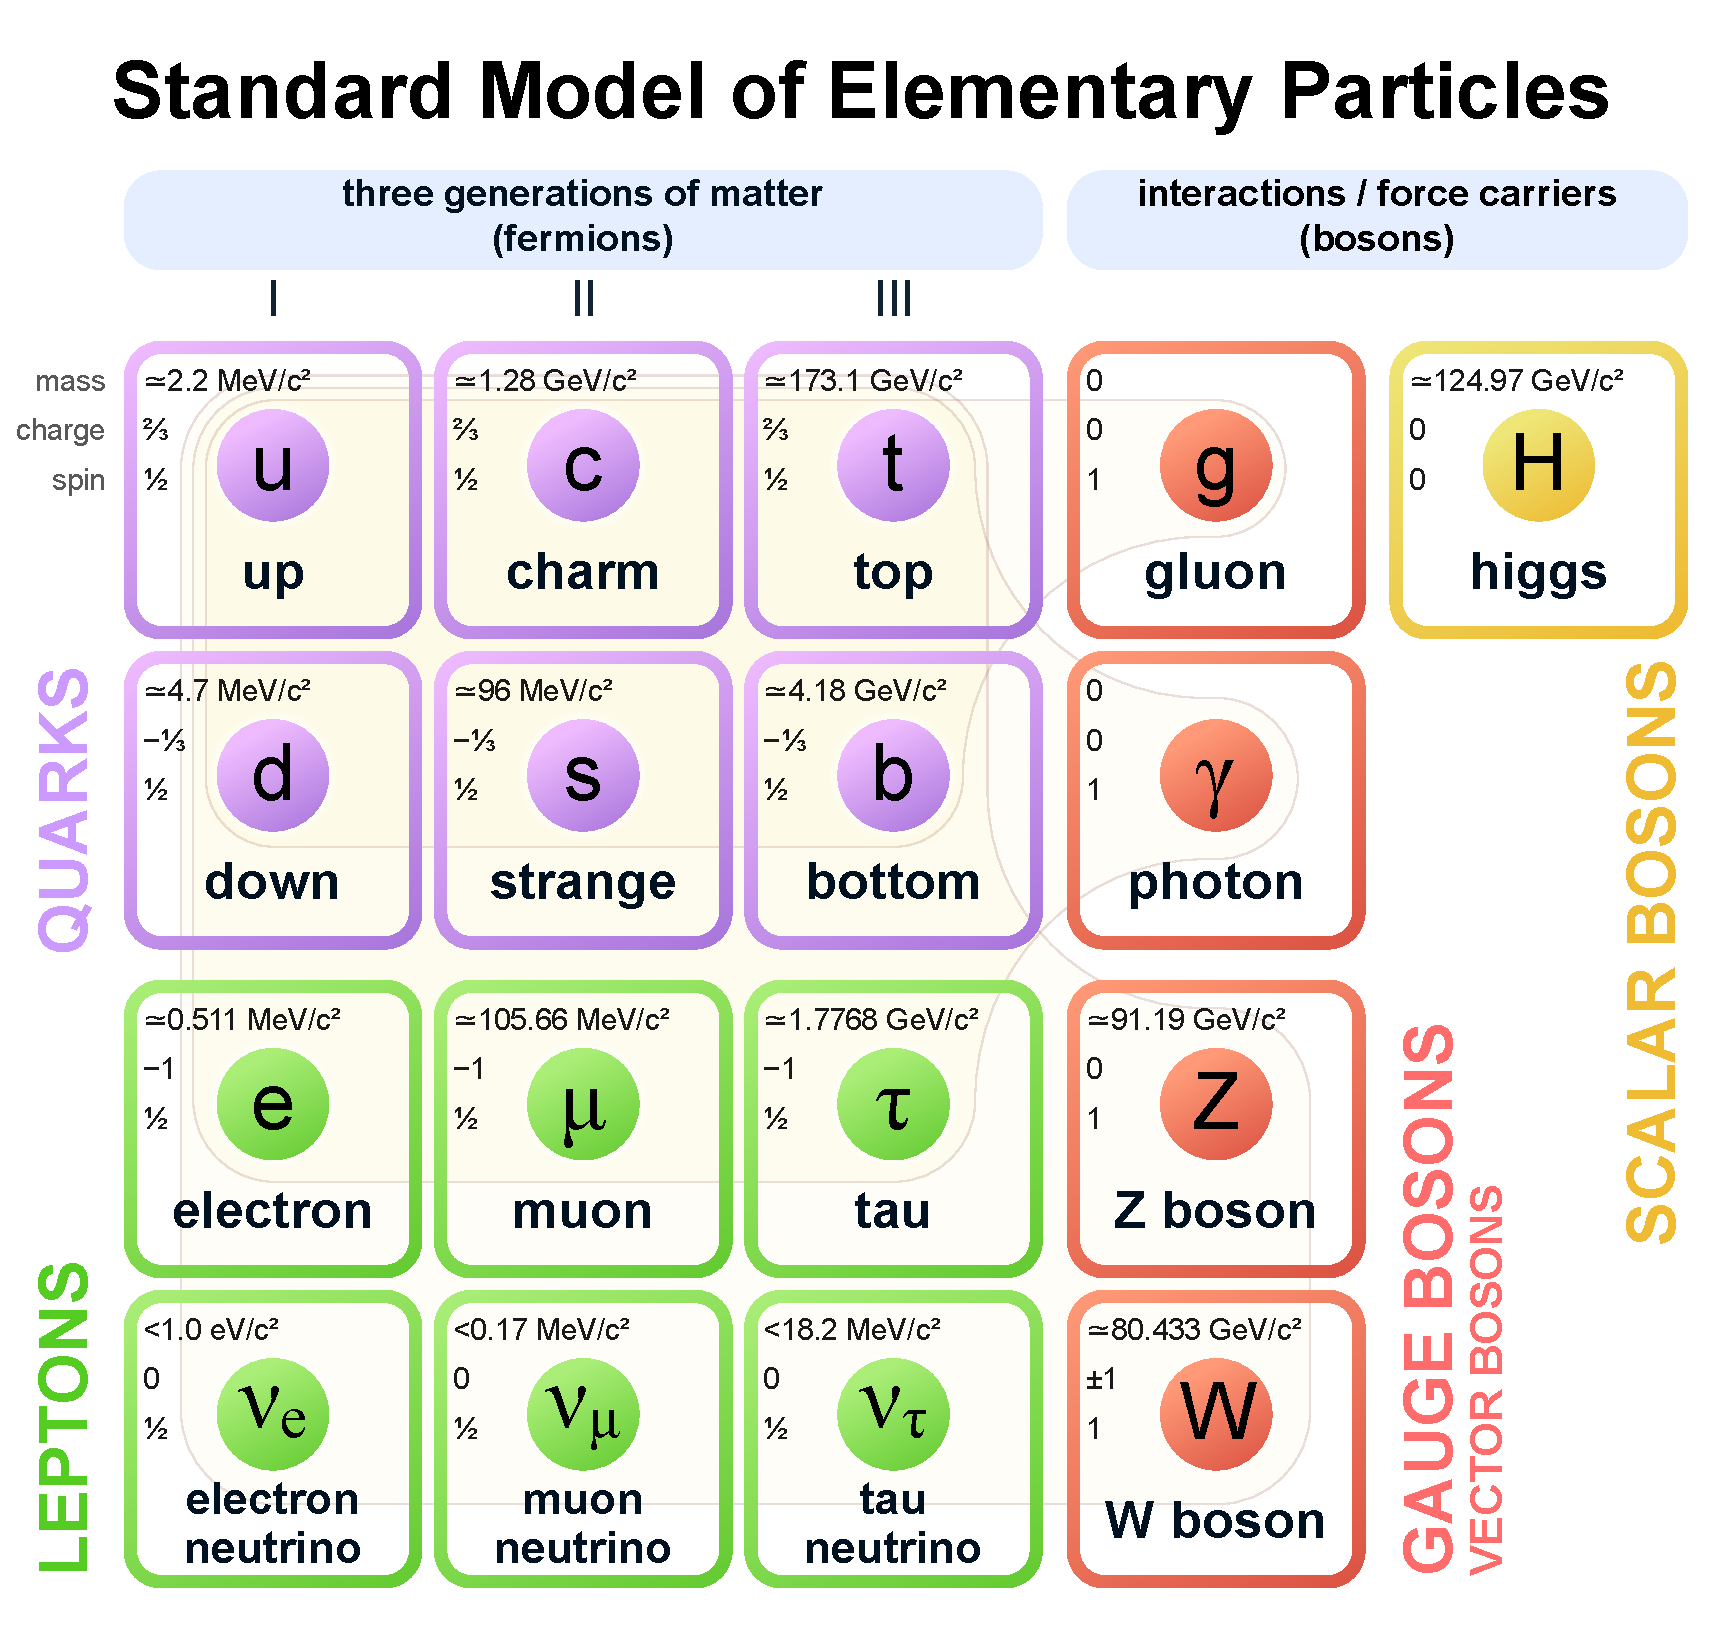
\includegraphics[width=0.9\textwidth]{fig_Theory/Standard_Model.pdf}
    \end{tabular}
    \caption{The Standard Model of Elementary Particle Physics
            }
    \label{Standard_Model}
  \end{center}
\end{figure}

\subsection{Fermions and Bosons}
In the SM, composite particles of matter are described in terms of their constituent elementary particles of half-integer spin, called fermions, which are particles of matter which are bound together by the exchange of fundamental, force-carrying particles of integer spin, called bosons. 

Fermions are further categorized into subgroups of quarks and leptons.
Leptons and quarks carry electric charge ($Q$) and therefore participate in the electromagnetic interaction.
Quarks additionally carry red ($R$), green ($G$), or blue ($B$) color charge, and so can also participate in the strong interactions.
Because of this property and the nature of QCD, quarks cannot exist in isolation, but instead can only be observed confined to colorless bound states called hadrons.
There are three so-called generations of fermions, and each generation is composed of both a pair of leptons and a pair of quarks, resulting in a total of twelve fermions: six quarks and six leptons.
Fermions of higher generations are more massive than those of the previous generation.
The up ($u$) and down ($d$) quarks, together with the electron ($e$) and electron neutrino ($\nu_e$) leptons, compose the first generation of fermions.
Both protons and neutrons are composed of different combinations of three up and down quarks; therefore, virtually all atomic matter is composed of only first generation fermions.
The second generation of fermions consists of the charm ($c$) and strange ($s$) quarks as well as the muon ($\mu$) and muon neutrino ($\nu_\mu$) leptons.
Finally, the third generation of fermions is composed of the top ($t$) and bottom ($b$) quarks (sometimes nicknamed truth and beauty), together with the tau ($\tau$) and tau neutrino ($\nu_\tau$) leptons.
The $e$, $\mu$, and $\tau$, referred to as "charged leptons", carry $Q = -1$, but the $\nu_e$, $\nu_\mu$, and $\nu_\tau$ neutrinos are electrically neutral.
The $u$, $c$, and $t$ quarks, referred to as "up-type," carry $Q = +\frac{2}{3}$, whereas the $d$, $c$, and $b$ quarks, referred to as "down-type," carry $Q = -\frac{1}{3}$.
Left-handed quarks and leptons additionally carry weak isospin ($I$ with third component $I_3$) and therefore participate in the weak interaction.
Left-handed charged leptons and down-type quarks carry $I_3 = +\frac{1}{2}$, while left-handed neutrinos and up-type quarks $I_3 = -\frac{1}{2}$.
Every fermion, i.e. denoted arbitrarily as $x$, has an anti-matter counterpart denoted $\Bar{x}$, that has the same mass as $x$, but opposite-signed quantum numbers.
The opposite-signed inversions of red, green and blue color charges are anti-red, anti-green and anti-blue, respectively.

The fundamental interactions of the SM are described by exchange of mediating force-carrying spin-1 gauge bosons.
Mathematically, these mediators arise from the gauge field group generators of the symmetry groups $U(1)$, $SU(2)$, and $SU(3)$.
The SM also includes a spin-0 scalar boson that is associated with a scalar field responsible for breaking the weak isospin symmetry of the electroweak interaction.

\subsection{The Electromagnetic Interaction}
The photon ($\gamma$) is the massless and electrically neutral gauge boson that mediates the electromagnetic interaction between electrically charged particles.
The electromagnetic interaction is described by QED with gauge symmetry group $U(1)$.
The electromagnetic coupling, i.e. the fine structure constant $\alpha_{EM} \approx \frac{1}{137}$, is significantly small relative to unity.
For the given process, the momentum of mediating virtual photons depend on the square of the momentum transfer, and therefore the coupling constant "runs," and the interaction becomes stronger (but still significantly smaller than unity) at higher values of momentum transfer.
As $\alpha_{EM} << 1$ even at higher values of momentum transfer, perturbative power series expansions in $\alpha_{EM}$ have proven to be extremely effective at explaining experimental results with QED.
Despite only providing approximate predictions, this effectiveness has made QED one of the most well-tested and successful theories in physics.

\subsection{The Weak Interaction}
The $W^\pm$ and $Z$ are massive gauge bosons that mediate the weak interaction between fermions carrying weak isospin ($I$ with third component $I_3$).
$W^\pm$ carries $Q = 0$, while $Z$ is electrically neutral.
Weak isospins of $I_3 = \pm 1$ ($I_3 = 0$) are carried by the $W^\pm$ ($Z$) bosons.
The $W^\pm$ and $Z$ boson masses are $\sim \SI{80.4}{\GeV}$ and $\sim \SI{91.2}{\GeV}$ respectively, resulting in their lifetimes, $\sim \SI{e-25}{\s}$, being incredibly short.
The short lifetimes limit the interaction ranges to be extremely small scales, as the distance these bosons can travel before decaying is very short.
The weak interaction is responsible for fermionic decay processes, such as nuclear radioactivity, is the only fundamental interaction that violates parity ($P$), charge conjugation parity ($CP$), and time-reversal ($T$) symmetries, and is described in the SM by gauge symmetry group $SU(2)$.
$Z$ bosons mediate the neutral weak interaction between same-flavor fermions, while $W^\pm$ bosons mediate the charged weak interaction between leptons of the same generation and can also flavor mix quarks of different generations.
Information about the conversion probabilities of flavor changing weak decays for quarks is encoded in the parameters of the Cabibbo-Kobayashi-Maskawa (CKM) matrix.

\subsection{The Strong Interaction}
Gluons ($g$) are massless gauge bosons that mediate the strong interaction between color charged particles.
The strong interaction is described by QCD with gauge symmetry group $SU(3)_C$.
While quarks (anti-quarks) carry color (anti-color) charge, gluons uniquely carry both color and anti-color charge, and therefore, gluons can interact with other gluons at trilinear and quartic self-interaction vertices.
There is a color octet of 8 different types of gluons, corresponding to 8 independent color state superpositions of the $3^2$ color/anti-color combinations.
One additional independent state exists mathematically, a color singlet carrying no color charge, but there is no experimental evidence for it and $SU(3)_C$ does not allow it.

The strong coupling $\alpha_S$ runs vigorously as the momentum transfer decreases, i.e. the interaction strength between quarks becomes stronger the further they are separated from each other.
This property of QCD results in color confinement, because before the energy between two separated quarks becomes arbitrarily large, a critical energy is reached for hadronization, in which a new quark/anti-quark pair is materialized from the energy of the mediating gluon.
Hadrons are classified by the flavor combinations of their valence quarks, but because quark interactions are mediated by gluons that can interact with themselves and split into quark/anti-quark pairs, there also exists a sea of virtual quarks and gluons within hadrons.
Protons and neutrons, colorless flavor combinations of three valence quarks, are categorized as baryons, whereas colorless flavor combinations of one valence quark and one valence anti-quark, such as pions and kaons, are categorized as mesons.
Experimental evidence for colorless flavor combinations of five valence quarks, categorized as pentaquarks, and colorless flavor combinations of two valence quarks and 2 valence anti-quarks, have also been reported in recent years.
Of all known hadrons, only the proton appears to be stable; with a mean life time constrained to be at least $10^34$ years, proton decay has never been observed.

Another consequence of the running of $\alpha_S$ is asymptotic freedom.
At higher and higher values of momentum transfer, $\alpha_S$ asymptotically approaches zero, i.e. quarks and gluons behave more like free particles at high energies.
At sufficiently high values of momentum transfer, such as those in hard scattering processes at hadron collider experiments, perturbative power series expansions in $\alpha_S$ become effective at explaining experimental results with QCD.

\subsection{The GWS Model, EWSB, and the BEH Mechanism}
At low energy energies, the electromagnetic and weak interactions are distinctly separate forces.
For energy scales beyond the unification energy $\sim$\SI{246}{\GeV}, electroweak theory unifies these two interactions into a single force described by a spontaneously broken Yang-Mills field with gauge symmetry group $SU(2)_L \otimes U(1)_Y$, generated by weak isospin ($I$) and weak hypercharge ($Y$).
In the Glashow-Weinberg-Salam (GWS) mopde, the $U(1)_Y$ group is mediated by a massless $B^0$ boson via the weak hypercharge field, and the $SU(2)_L$ group is mediated by massless $W^1$, $W^2$, and $W^3$ bosons via the weak isospin fields.
The subscript $L$ indicates that only left-handed fermion doublets carry isospin, while the right-handed singlets do not.

In the SM, the $\gamma$, $Z$, and $W^\pm$ bosons arise from the Brout-Englert-Higgs (BEH) mechanism spontaneously inducing electroweak symmetry breaking (EWSB) in the GWS model.
Mathematically, electric charge $Q = I_3 + \frac{1}{2} Y$ arises as a specific linear combination of weak isospin and hypercharge.
Electrically neutral $\gamma$ and $Z$ bosons arise from mixed states of the $B^0$ and $W^3$ bosons:
\begin{align}
\left(\begin{array}{c}
\gamma \\
Z^0
\end{array}\right)=\left(\begin{array}{cc}
\cos \theta_{\mathrm{W}} & \sin \theta_{\mathrm{W}} \\
-\sin \theta_{\mathrm{W}} & \cos \theta_{\mathrm{W}}
\end{array}\right)\left(\begin{array}{c}
B \\
W_3
\end{array}\right)
\label{}
\end{align}
where $\theta_{\mathrm{W}}$ is the Weinberg weak mixing angle.
Electrically charged $W^\pm$ bosons arise from linear combinations of the $W^1$ and $W^2$ bosons:
\begin{align}
W^{\pm}=\frac{1}{\sqrt{2}}\left(W_1 \mp i W_2\right).
\label{}
\end{align}

In the GWS model, local gauge symmetry prohibits mass terms in the Lagrangian for gauge bosons (Goldstone's theorem), but the $W^\pm$ and $Z$ bosons are experimentally known to have large masses.
To both resolve this discrepancy and induce EWSB, the BEH mechanism adds a complex scalar $SU(2)$ doublet field $\phi$ to the SM that permeates all of space:
\begin{align}
\phi=\left(\begin{array}{l}
\phi^{+} \\
\phi^0
\end{array}\right)=\frac{1}{\sqrt{2}}\left(\begin{array}{l}
\phi_1+i \phi_2 \\
\phi_3+i \phi_4
\end{array}\right)
\end{align}
with potential energy:
\begin{align}
V(\phi) = -\mu^2 \phi^{\dagger} \phi + \lambda\left(\phi^{\dagger} \phi\right)^2
\end{align}
The BEH potential, colloquially referred to as a Mexican-hat potential, has global $U(1)$ and $SU(2)$ symmetries.
The energy at the center of the potential is higher than at a ring of equivalent vacuum states with vacuum expectation energy $\langle\phi\rangle=\sqrt{\frac{\mu^2}{2 \lambda}} \equiv \frac{v}{\sqrt{2}}$ that breaks the electroweak gauge symmetry.
Without loss of generality, $\phi$ can be parameterized with an expansion around $v$, by introducing scalar field $h$, and with a unitary gauge transformation:
\begin{align}
\phi=\frac{1}{\sqrt{2}}\left(\begin{array}{c}
0 \\
v+h
\end{array}\right)
\end{align}
Of the original four degrees of freedom in the complex scalar $SU(2)$ doublet field, the electrically charged $\phi_1$ and $\phi_2$ are absorbed to generate mass terms in the Lagrangian for the $W^\pm$ bosons, while the electrically neutral $\phi_4$ term is absorbed to generate mass for the $Z$ boson.
The remaining electrically neutral $\phi_3$ is split into $v$ and the new field $h$, with quantum numbers $I_3 = \frac{-1}{2}$ and $Y = +1$ ($Q = 0$), which manifests as the physical Higgs ($H$) boson, a scalar boson that mediates interactions between the fermions and the BEH field, endowing them with mass proportional their Yukawa coupling constant $y_f$.
The Higgs boson was experimentally discovered in 2012 jointly by the CMS and ATLAS LHC experiments at CERN; Peter Higgs and François Englert received the 2013 Nobel Prize in Physics for their theoretical predictions, while Robert Brout passed away in 2011.

\section{Beyond the Standard Model}
The SM is a central pillar of modern particle physics, many of its predictions have been confirmed by innumerable experiments to exquisite precision, and is considered to be one of the most mature and successful theories in all of science.
Despite its success, there are a number of known physical phenomena that are not explained by the SM, and it is considered to be an effective theory up to some scale $\Lambda \approx \si{\TeV}$.
All theoretical and experimental investigations that are beyond the current understanding of the Standard Model of particle physics are collectively referred to as Beyond the Standard Model (BSM).

Following the example of electroweak unification, theoretical frameworks that aim to unify the strong and electroweak interactions into a single, unified force are referred to as Grand Unification Theories (GUT).
While the scale of electroweak unification is $\sim \SI{e2}{\GeV}$, the scale of grand unification is estimated to be $\sim \SI{e14}{\GeV} - \SI{e16}{\GeV}$.
Given the extreme energy requirements, it is unsurprising that no experimental evidence for GUT predictions have been found yet at energy scales accessible to modern particle accelerator experiments.

The the theoretical explanation for the experimental observation of neutrino oscillations predicts that the neutrino masses are non-zero.
However. the SM predicts that neutrinos should be massless particles. 

The discovery of the Higgs boson with mass $\sim \SI{125}{\GeV}$ has creating an inconsistency in the SM known as the "Heirarchy Problem."
Virtual loop corrections to the Higgs boson mass generate quadratic divergences.
Calculating a predicted Higgs boson mass compatible with the observed value requires unnatural fine-tuning, highlighting the likelihood of New Physics (NP) between the electroweak scale and the Planck scale, natural scale of quantum gravity.

The most glaring absence from the SM framework is the gravitational interaction between massive objects.
A theory that reduces all four physical interactions into a single, unified theory is colloquially referred to as the "Theory of Everything," and it is the holy grail of particle physics.
Einstein's general theory of relativity (GR) is a classical theory of gravitation that describes the force of gravity as resulting from the curvature of spacetime caused by the presence of massive objects.
All attempts to unify the SM and GR have failed, and the two are considered to be separate and incompatible theories.
A major focus of current theoretical physics research is centered around the formulation of a QFT that describes the gravitational interaction, but a common feature of these theories is that they are non-renormalizable.
Theories of quantum gravity predict the existence of a massless, spin-2 gauge boson dubbed the graviton.
Experimentally however, gravity is $\sim 10^{24}$ times weaker than the weak interaction, and the lack of experimental sensitivity makes it extremely difficult to verify the predictions of these theories.

There are astrophysical and cosmological observed physical phenomena as well that are not explained by the SM.
The asymmetry between the observed matter and anti-matter in the universe remains unexplained by the SM.
Based on the assumption that the universe started with equal quantities of matter and anti-matter, the conditions required for baryogenesis, i.e. the generation of a cosmological excess of baryons over anti-baryons, include baryon number violation, CP-violation, and charge conjugation symmetry ($C$) violation.
Sources of CP-violation in the SM via the weak interaction are not sufficient to account for the extreme asymmetry and baryon number is not violated whatsoever.
CP-violation via the strong interaction is mathematically allowed in the SM, but the relevant parameters have been inexplicably measured to be extremely small (strong CP problem).
Astronomical observations of gravitational lensing effects and in the velocity of rotation curves of spiral galaxies suggest that $85 \%$ of all observed matter in the universe is dark matter, an unknown form of matter that has its namesake in that it does not emit, absorb or reflect electromagnetic radiation, and thus can only be indirectly inferred through its gravitational effects on visible matter.
Although dedicated dark matter detection experiments exist that search for Weakly Interacting Massive Particles (WIMP), conclusive direct observation of dark matter WIMPs has not yet occurred.
Cosmological observations of galaxies also indicate that the expansion of space is accelerating.
The cause of this expansion is unknown, but it is attributed to an enigmatic form of energy, dubbed dark energy, that is thought to be responsible for $73 \%$ of the total energy density of the universe.

Many BSM extensions have been made that predict new elementary particles that, depending on their properties and stability, could explain dark matter.
Perhaps the most popular of these extensions is Supersymmetry (SUSY), which predicts the existence of superpartners for every fermion and boson in the SM by adding terms to the Lagrangian and make it symmetric with respect to matter and field-mediating particles.
SUSY can resolve the hierarchy problem by providing superpartner terms that cancel the quadratic divergences to the Higgs boson mass from heavy virtual particles.
Despite compelling arguments for why the predicted superpartners could be in reach of LHC experiments, the lack of experimental evidence for SUSY has led to a resurgence of interest in alternative BSM models to resolve these open questions.

SM Effective Field Theory (SMEFT) is a model-independent extension of the Standard Model which uses a systematic product expansion in terms of higher-dimensional operators to describe the effects of NP at higher energy scales.  
Due to its agnostic construction, SMEFT allows for a broad range of possibilities for NP, which is parameterized as coefficients of the operators in the expansion, referred to as Wilson coefficients.






% Summary and/or conclusions are optional but often used.
% The summary and/or conclusions often are the last
% the last major division(s) of the text.
% Reference: TM2017 page 32.




% Appendices are optional.  Not all theses contain appendices.
% An appendix is used for supplementary illustrative material,
% original data, computer programs, and other material that is not
% necessarily appropriate for inclusion within the text of your
% thesis.
% Reference: TM2017 page 33.
%
% Use ``\appendix'' for one appendix or ``\appendices'' for more than
% one appendix.
\appendices

\ProvidesFile{appendices/ap-TriggerSF.tex}

\chapter{Measurements of Trigger Scale Factors for Dilepton Final States of \ttbar Events}

\section{Overview and Motivation}
Here is presented the measurements of the trigger efficiencies and corrective scale factors that were used by virtually all CMS Run II measurements analyzing \ttbar events that decay via the dileptonic mode with \ee, \emu, \mumu final states.  
The methods used for the measurements and the determination of systematic uncertainties, were approved by the EGamma and Muon CMS Physics Object Groups, because of the inclusion of electron and muon objects respectively, as well as by the CMS Top Quark Physics Analysis Group.

Trigger efficiencies measure the ability of the CMS trigger system to select potentially interesting events for further analysis.
Differences between the observed trigger efficiencies of data recorded by the detector and the expected trigger efficiencies of simulated data can bias measured physics results, and these differences are corrected via trigger efficiency scale factors that are applied to the trigger efficiencies of simulated data, so that they match the observed trigger efficiencies of recorded data.
Trigger efficiency corrective scale factors are calculated as:
\begin{eqnarray}
SF = \frac{\varepsilon^{data}}{\varepsilon^{MC}}
\label{SF}
\end{eqnarray}
where $\varepsilon^{data}$ and $\varepsilon^{MC}$ are trigger efficiencies for data and Monte Carlo simulated data, respectively.

The method used to measure the dilepton trigger efficiencies utilizes a set of cross-triggers, that are weakly correlated with the dilepton triggers, to count the number of events passing the cross-trigger and \ttbar dilepton final state event selection criteria (denominator), and from that set count also the subset that passes the dilepton triggers (numerator).
Missing transverse energy (\MET) triggers are shown to be minimally correlated with the dilepton triggers, and they provide sufficient statistics for low statistical uncertainties, so they are used as the cross-triggers for these measurements. 
The trigger efficiencies, for both data and Monte Carlo simulated data, are thus calculated as: 
\begin{eqnarray}
\varepsilon = \frac{N_{Events ~passing ~dilepton ~selection, ~\MET ~triggers, ~and ~dilepton ~triggers}}{N_{Events ~passing ~dilepton ~selection ~and ~\MET ~triggers}}
\label{efficiency}
\end{eqnarray}
where, in addition to passing the triggers, events have to also pass the event selection criteria for the appropriate dilepton channel. 

The dilepton trigger efficiency corrective scale factors are measured, separately in the \ee, \emu, \mumu channels, as 1-Dimensional and 2-Dimensional functions of leading and sub-leading lepton \pT.
The 2-Dimensional scale factors are the set recommended to be used by by virtually all CMS Run II measurements analyzing \ttbar events that decay via the dileptonic mode with \ee, \emu, \mumu final states.

\section{Data Sets and Triggers}
The measurements were original performed using pre-Ultra Legacy CMS data sets, but were repeated using the Ultra Legacy sets, which are preserved for long term access, are comprehensively documented, designed to be useful for a wide range of studies, and include high-level physics objects just as reconstructed leptons, jets, and missing transverse energy.
The data streams were collected by the CMS experiment in 2016, 2017 and 2018, and correspond to a combined integrated luminosity of \lumivalueRuniiUL.
The 2016 data set is separated into preVFP and postVFP, partitioning the year into the periods before and after Heavily Ionizing Particle Mitigation (HIPM) was implemented.
The lists of triggers for each of the three years were provided in collaboration with the CMS Top Quark Physics Analysis Group trigger experts; both single lepton and dilepton triggers are used in order to maximize the trigger efficiency. 

\section{Object and Event Selection}
The dilepton final state of \ttbar events is characterized by the presence of at least two high-\pT isolated leptons with opposite electric charge, large missing transverse energy (\MET), and two jets resulting from the hadronization of bottom quarks.
The identification and reconstruction of the different objects is performed using the particle-flow (PF) event-reconstruction algorithm, which combines information from all the raw sub-detector signals to accurately identify and reconstruct individual particle objects for each event. 
\subsection{Electrons}
Electron candidates are selected from the reconstructed Gaussian Sum Filter {GSF) electrons with $\pT > \SI{15}{\GeV}$ and $\abs{\eta_{SuperCluster}}<$ 2.4, removing the barrel-endcap gap 1.4442 $< \abs{\eta_{SuperCluster}}<$ 1.566. 
Selected electrons must to pass the tight identification tracking requirements, including relative isolation, as recommended by the CMS EGamma Physics Object Group.
Corrections to scale the raw energy measurements and smear the electron resolutions, to match the accuracy and precision of reconstructed electrons in MC simulated data to those in recorded data, are also applied.
\subsection{Muons}
Particle-Flow (PF) muons selected for this measurement are required to be reconstructed as Global Muons, relatively isolated, with $\pT > \SI{15}{\GeV}$ and $\abs{\eta}<$ 2.4, and to be identified as passing tight identification tracking criteria recommended by the CMS Muon Physics Object Group.
Corrections to scale the raw energy measurements and smear the muon resolutions, to match the accuracy and precision of reconstructed muons in MC simulated data to those in recorded data, are also applied.
\subsection{Jets}
Particle candidates found by the PF algorithm are clustered into jets using the anti-kT algorithm with distance parameter $R = 0.4$ (AK4). 
Selected jets should have $\pT > \SI{30}{\GeV}$, $\abs{\eta} <2.4$, and pass tight jet identification requirements recommended by CMS Jet-MET Physics Object Group.
In order to remove overlap of selected jets with the selected leptons, jet objects within $\Delta R(jet,lepton) < 0.4$ of selected leptons are not counted, where $\Delta R$ is defined as the square root of the pseudorapidity difference and the azimuthal difference, added in quadrature, and is invariant under longitudinal Lorentz boosts.
\subsection{Missing Transverse Energy}
In order to reduce the instrumental noise in the detector, \MET filters are applied as is recommended by CMS Jet-MET Physics Object Group.
An event selection requirement of $\MET > 100$ is included because of the high threshold of \MET triggers.
\subsection{Event Selection Criteria}
Events with exactly two high-\pT isolated PF leptons (electrons or muons) with opposite electric charge, PF leptons (electrons or muons) are selected. 
Both electrons and muons are required to have $\abs\eta < 2.4$, with $\pT > \SI{25}{\GeV}$ ($\pT > \SI{15}{\GeV}$) for the leading (sub-leading) lepton.  
The invariant mass of the two leptons is required to be greater than \SI{20}{\GeV}.  
Selected events are required to have at least one jet passing the loose working point of the DeepCSV b-tagging algorithm.

\section{Statistical and Systematic Uncertainties}
For the 2-Dimensional trigger efficiency scale factor measurements, the systematic uncertainties are added in quadrature with the statistical uncertainties for the final total uncertainties in each bin. 
For the 1-Dimensional trigger efficiency scale factor measurements, the sums in quadrature of the systematic uncertainties are plotted as a hashed uncertainty band for each bin, while the statistical uncertainties are shown as an independent error bar on the data points.
\subsection{Statistical Uncertainties}
The asymmetric statistical uncertainty for measured trigger efficiencies is determined using Clopper-Pearson intervals ~\cite{bib:Cousins:2009kz}.
This is in general a conservative method, since Clopper-Pearson intervals have the property that the actual coverage is at least as big as the nominal one for any population portion. 
It is also described in the statistics section of the Particle Data Group (PDG) book ~\cite{bib:PDG}.

The asymmetric statistical uncertainty for measured scale factors $T=(X / m) /(Y / n)$ is determined using the method recommended by Katz et al. for ratios of efficiencies, in which $\ln (T)$ is approximately normally distributed \cite{bib:10.2307/2531405}. 
The estimated variance is  $\hat{\sigma}^{2}=(1 / x)-(1 / m)+$ $(1 / y)-(1 / n)$ and an approximate two-sided $1 - \alpha$ confidence interval ($1 \sigma: 0.6827 = 1 - 0.3173$) is given by $\left\{t \exp \left(-\xi_{1-\alpha / 2} \cdot \hat{\sigma}\right), t \exp \left(\xi_{1-\alpha / 2} \cdot \hat{\sigma}\right)\right\}$ where $\xi_{1-\alpha / 2}$ is the $1-\frac{1}{2} \alpha$ fractile of the standard normal distribution, and $t$, $x$, and $y$ are the observed values of $T$, $X$, and $Y$ respectively.  
For the extreme cases in which $x = m$ and $y = n$, $x$ and $y$ are replaced with $x = m - 1/2$ and $y = n - 1/2$.
\subsection{Systematic Uncertainties}
The sources of systematic uncertainties are as follows:
\subsubsection{Event Topology}
In order to estimate the effect of event environment on the trigger scale factors, the data and MC samples are divided into independent regions using number of jets and number of vertices, and scale factors are computed separately in each region. 
An envelope of the largest bin-by-bin differences with respective to the nominal, is taken from the two partitions for number of jets and number of vertices independently.
The final event topology systematic uncertainty in each bin is the sum in quadrature of those two independent sources.
The number of jets distributions is relatively stable for different luminosity conditions during Run II, and the number of jets partition is [$< 3$, $\geq\ 3$] for all three eras.
However, the number of primary vertices distributions are more strongly dependent on the luminosity conditions and a different number of vertex partition is chosen for each era such that roughly the same percentage of MC events are below the partition.
For 2016, 2017, and 2018, the number of vertices partition are [$< 20$, $\geq 20$], [$< 30$, $\geq 30$], and [$< 30$, $\geq 30$] respectively.
\subsubsection{Dependence on Era}
The bin-by bin differences between the nominal measurement of the scale factor and a luminosity-weighted combination of scale factors measured for the individual runs in each era is taken as another source of systematic uncertainty.
\subsubsection{Correlations between \MET and dilepton triggers}
We estimate the correlation factor $(\alpha)$ between MET and dilepton triggers in \ttbar MC events by finding the fraction of events passing only the MET triggers ($\epsilon_{trigMET}^{MC}$), only the dilepton triggers ($\epsilon_{trigDL}^{MC}$) and passing both of them ($\epsilon_{trigDL,trigMET}^{MC}$): 
\begin{eqnarray}
\alpha=\frac{\epsilon_{trigDL}^{MC} \times \epsilon_{trigMET}^{MC}}{\epsilon_{trigDL,trigMET}^{MC}} \, .
\label{alpha}
\end{eqnarray}
If \MET and dilepton triggers are independent with no correlation, then $\epsilon_{trigDL,trigMET}^{MC} = \epsilon_{trigDL}^{MC} \times \epsilon_{trigMET}^{MC}$ or $\alpha = 1$ ($P\{A\cap B\} = P\{A\} \times P\{B\}$).
The fraction $(\alpha)$ is determined for each channel and data set from equation \ref{alpha} and its difference from 1 is found to be small for all triggers studied. 
Since these values are negligible with respect to the other systematic uncertainties, they are not added in quadrature for the final total uncertainty. 
Values of $\alpha$ as a function of leading and sub-leading lepton \pT, eta, and phi, as well as MET, number of jets, and number of vertices are shown in ~~~. 

\newpage
\section{Results}

\subsection{Trigger Efficiencies and Scale Factors: 2016preVFP}
\label{TrigSFResults2016preVFP}

\begin{figure}[h]
  \begin{center}
    \begin{tabular}{ccc}
      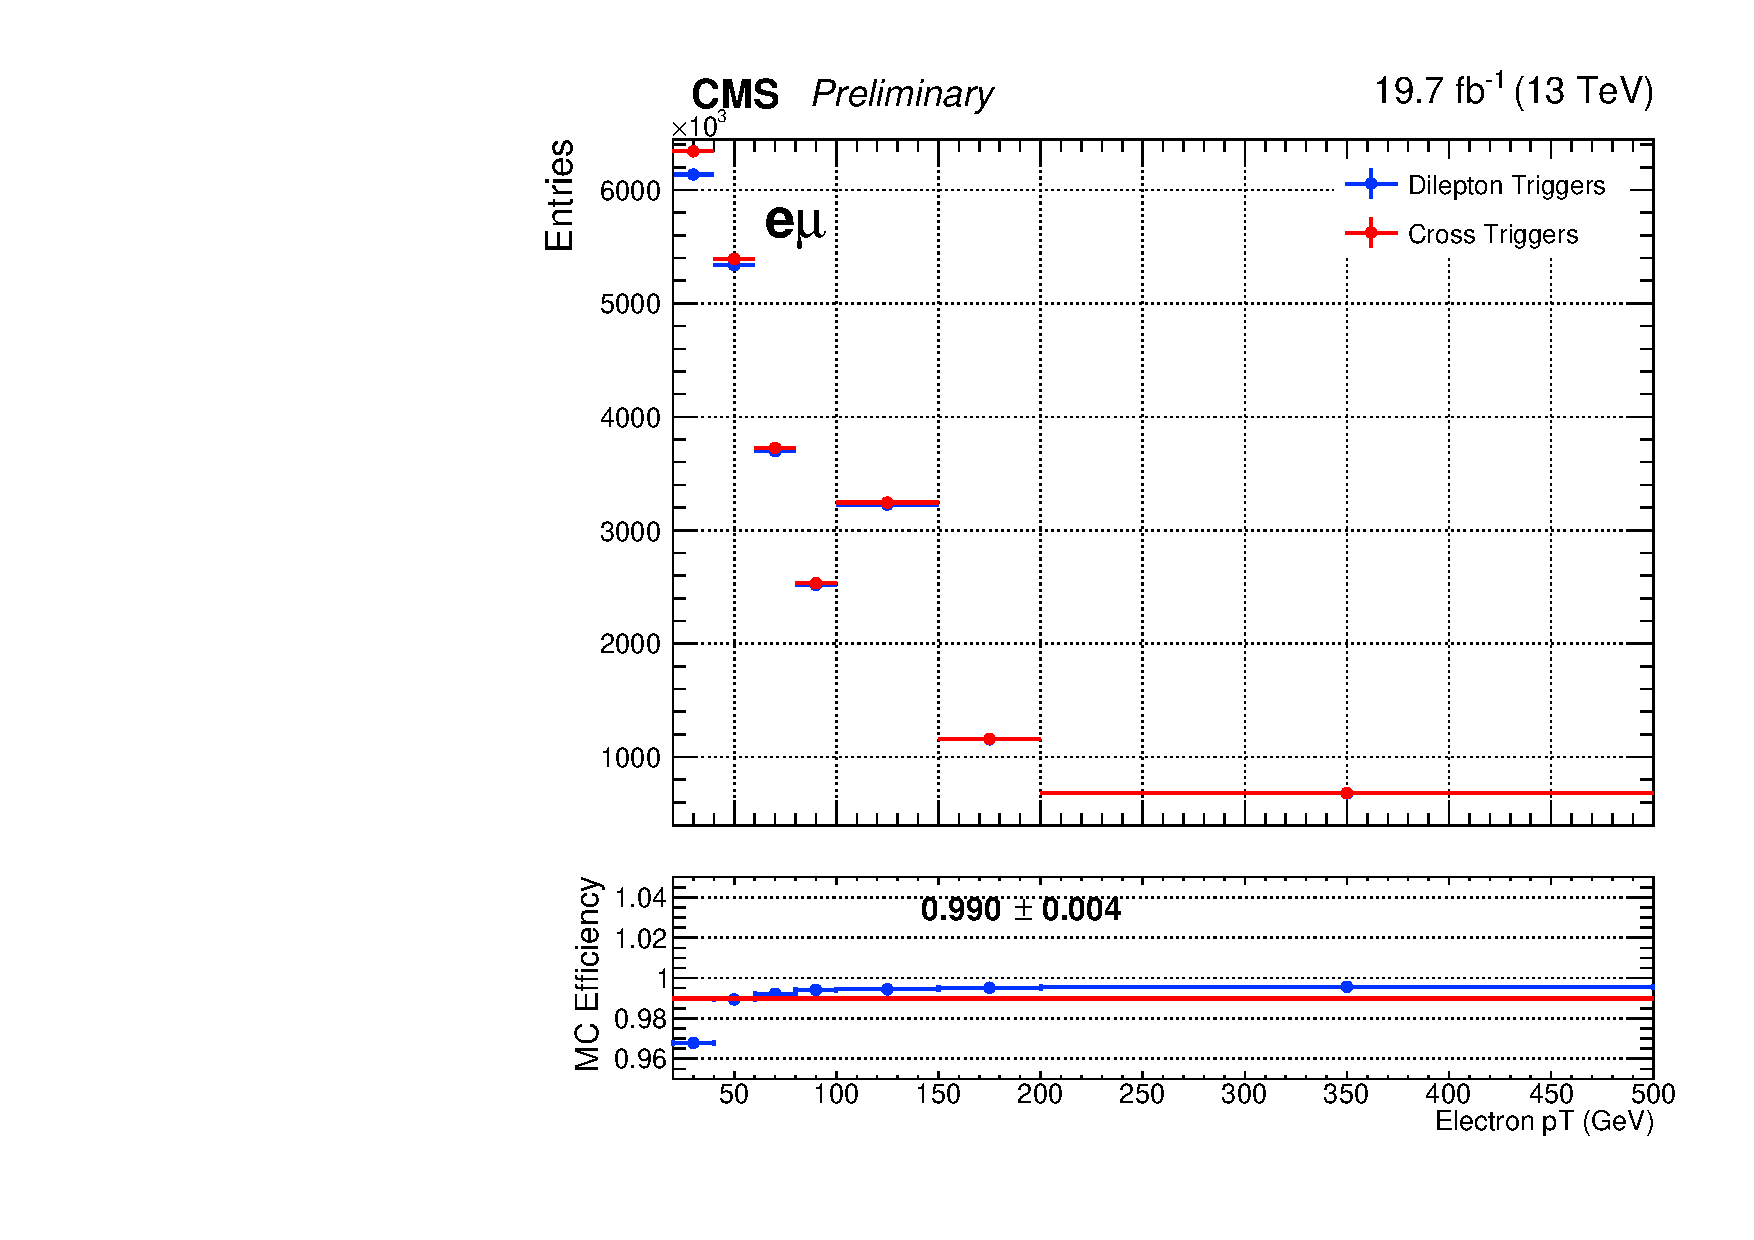
\includegraphics[width=0.32\textwidth]{fig_2016preVFP_TrigSF/g_lepApt_emu_MC.pdf}
      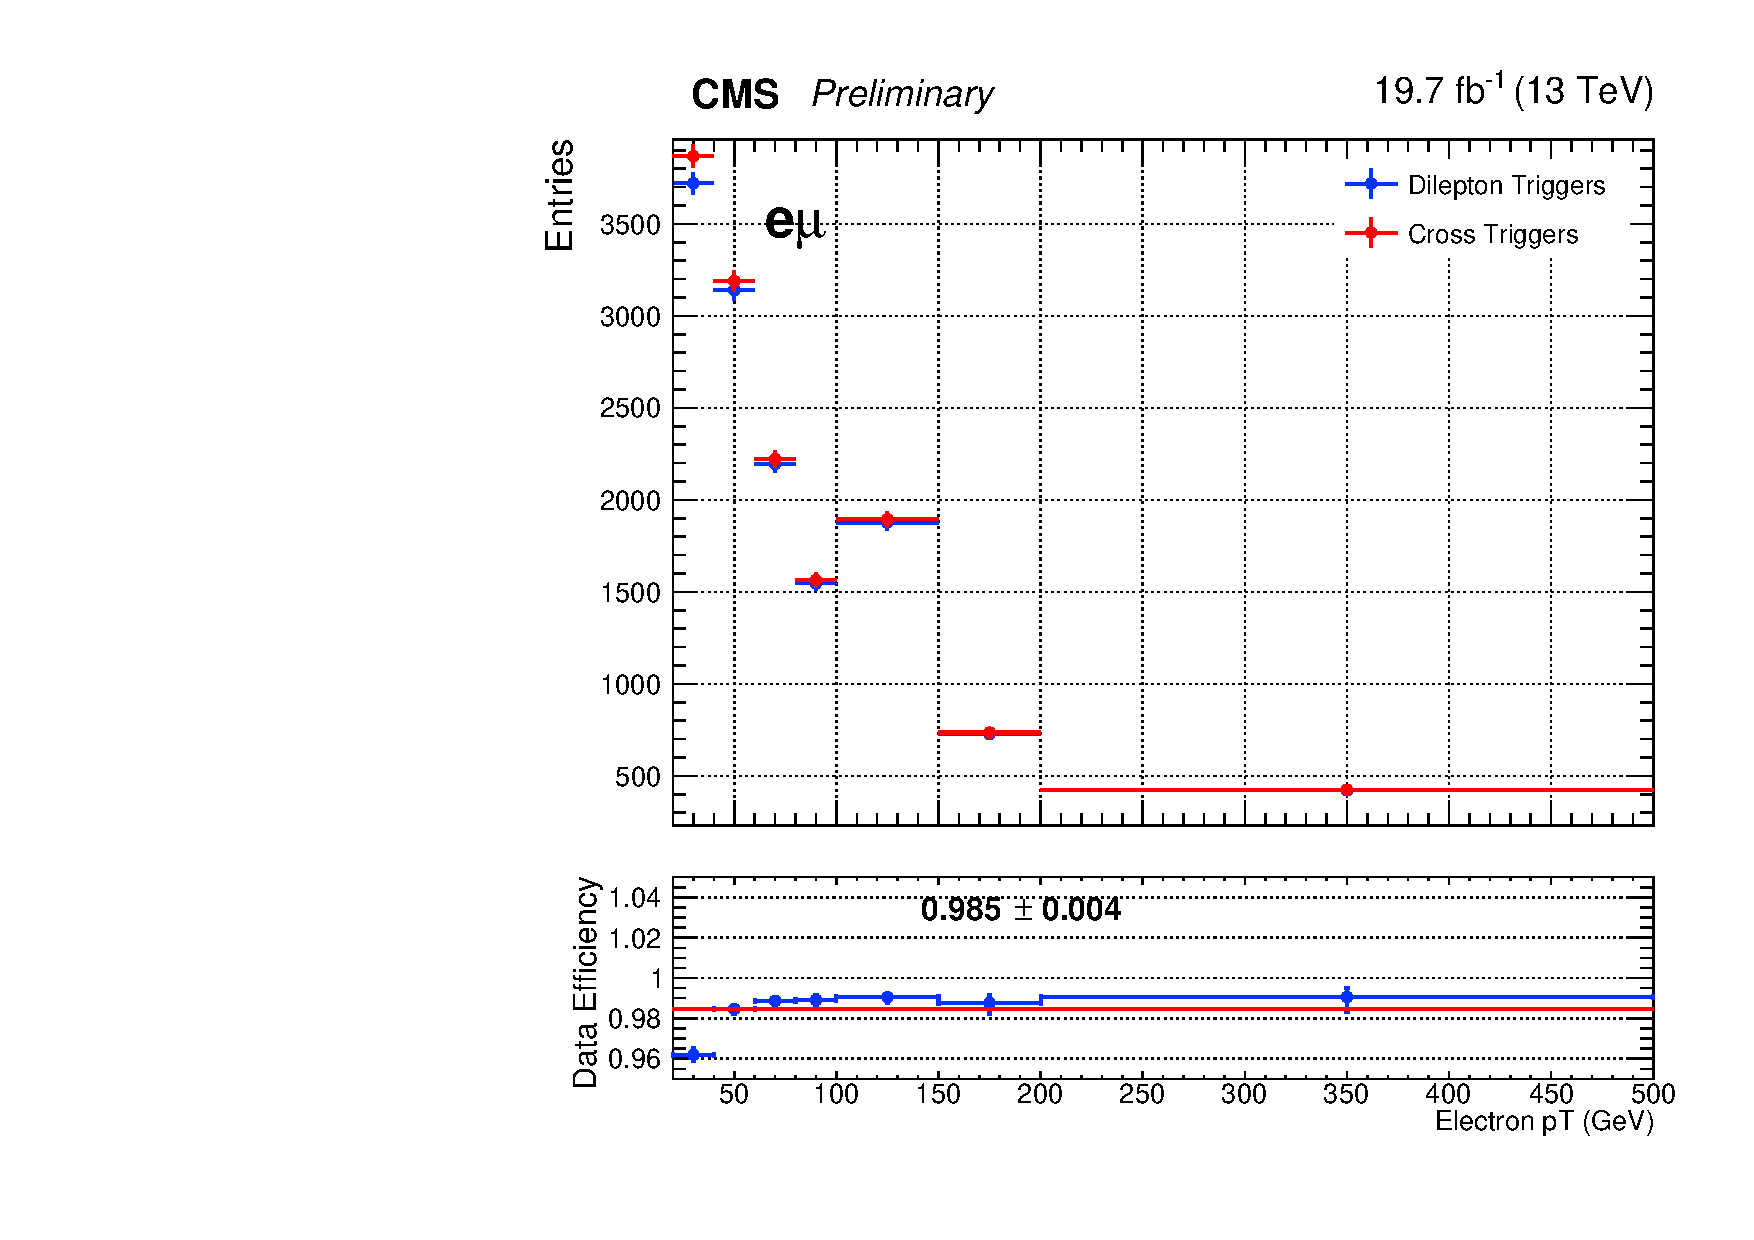
\includegraphics[width=0.32\textwidth]{fig_2016preVFP_TrigSF/g_lepApt_emu_data.pdf}
      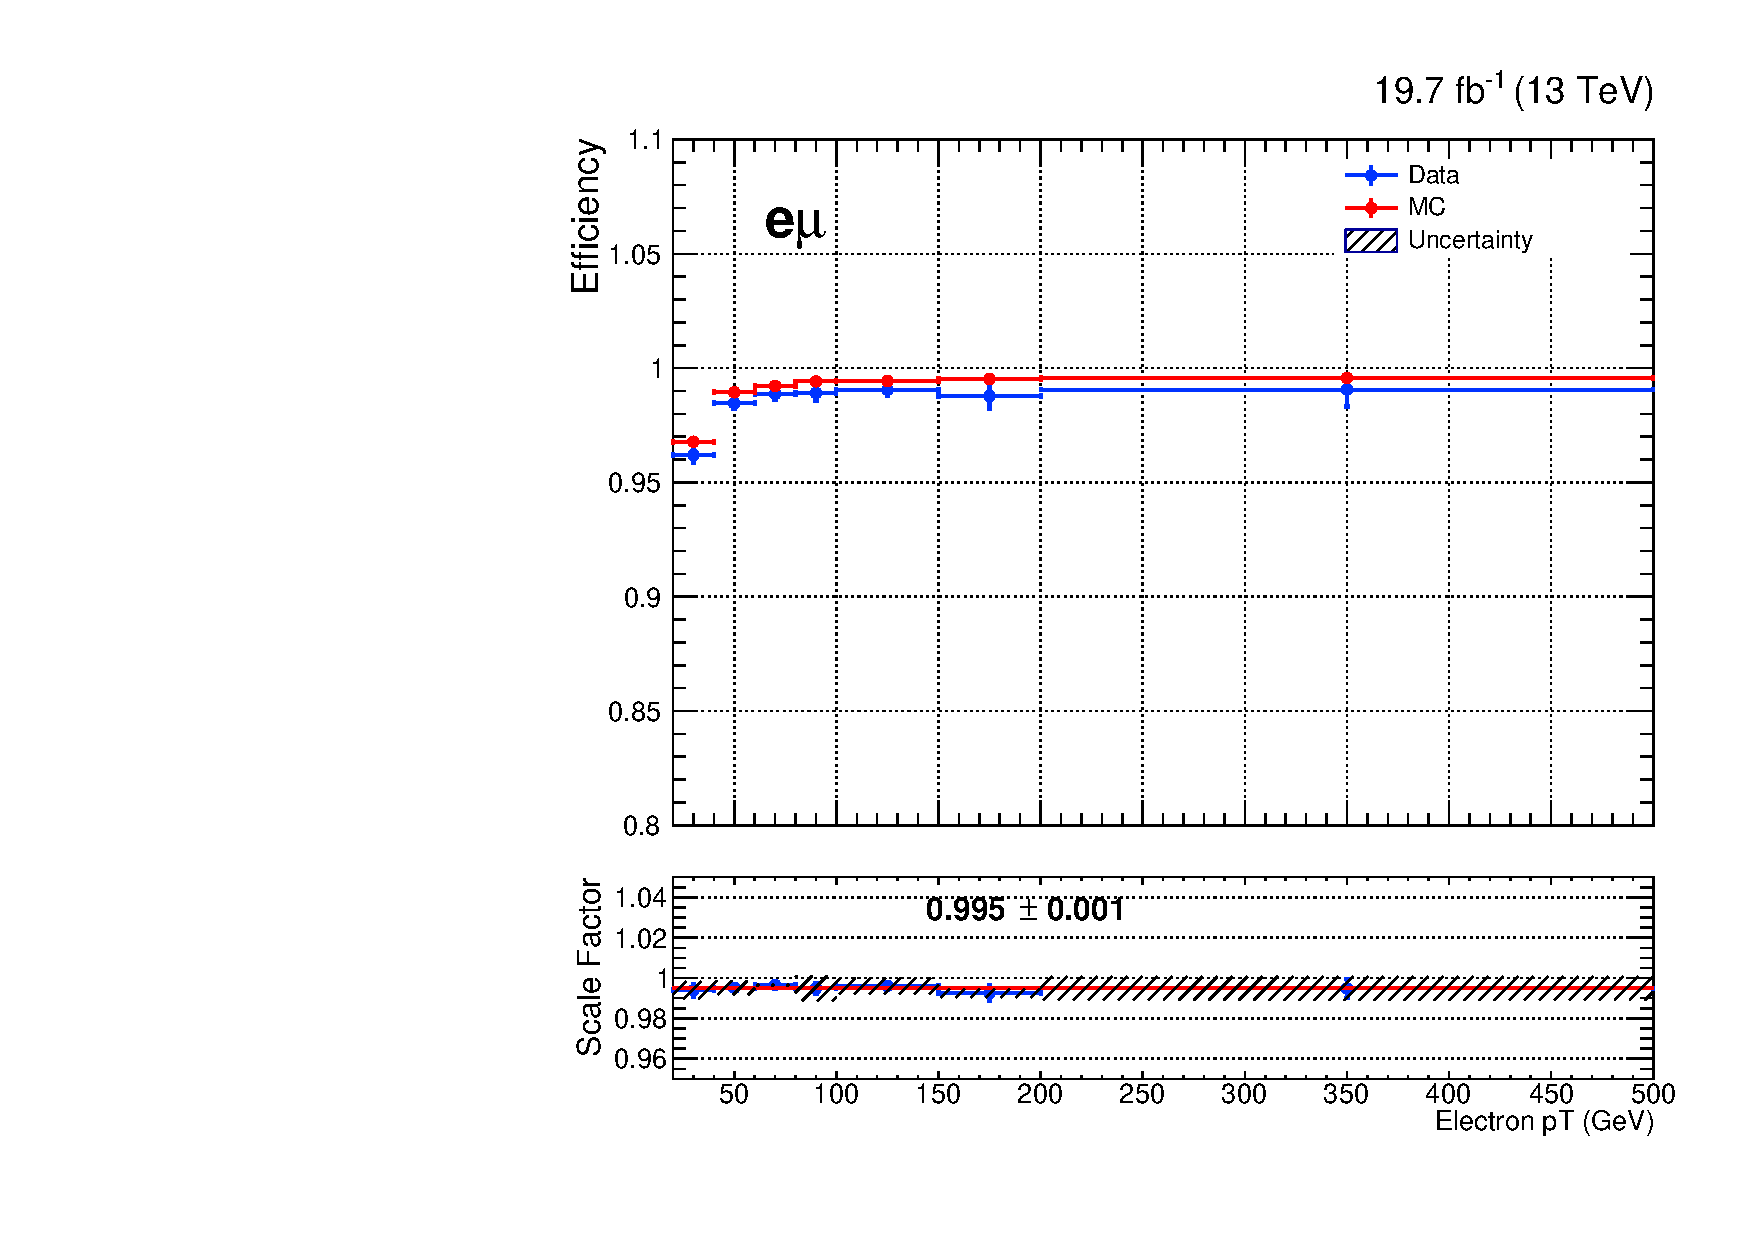
\includegraphics[width=0.32\textwidth]{fig_2016preVFP_TrigSF/g_emu_lepApt_FullSystUncBand.pdf}\\
      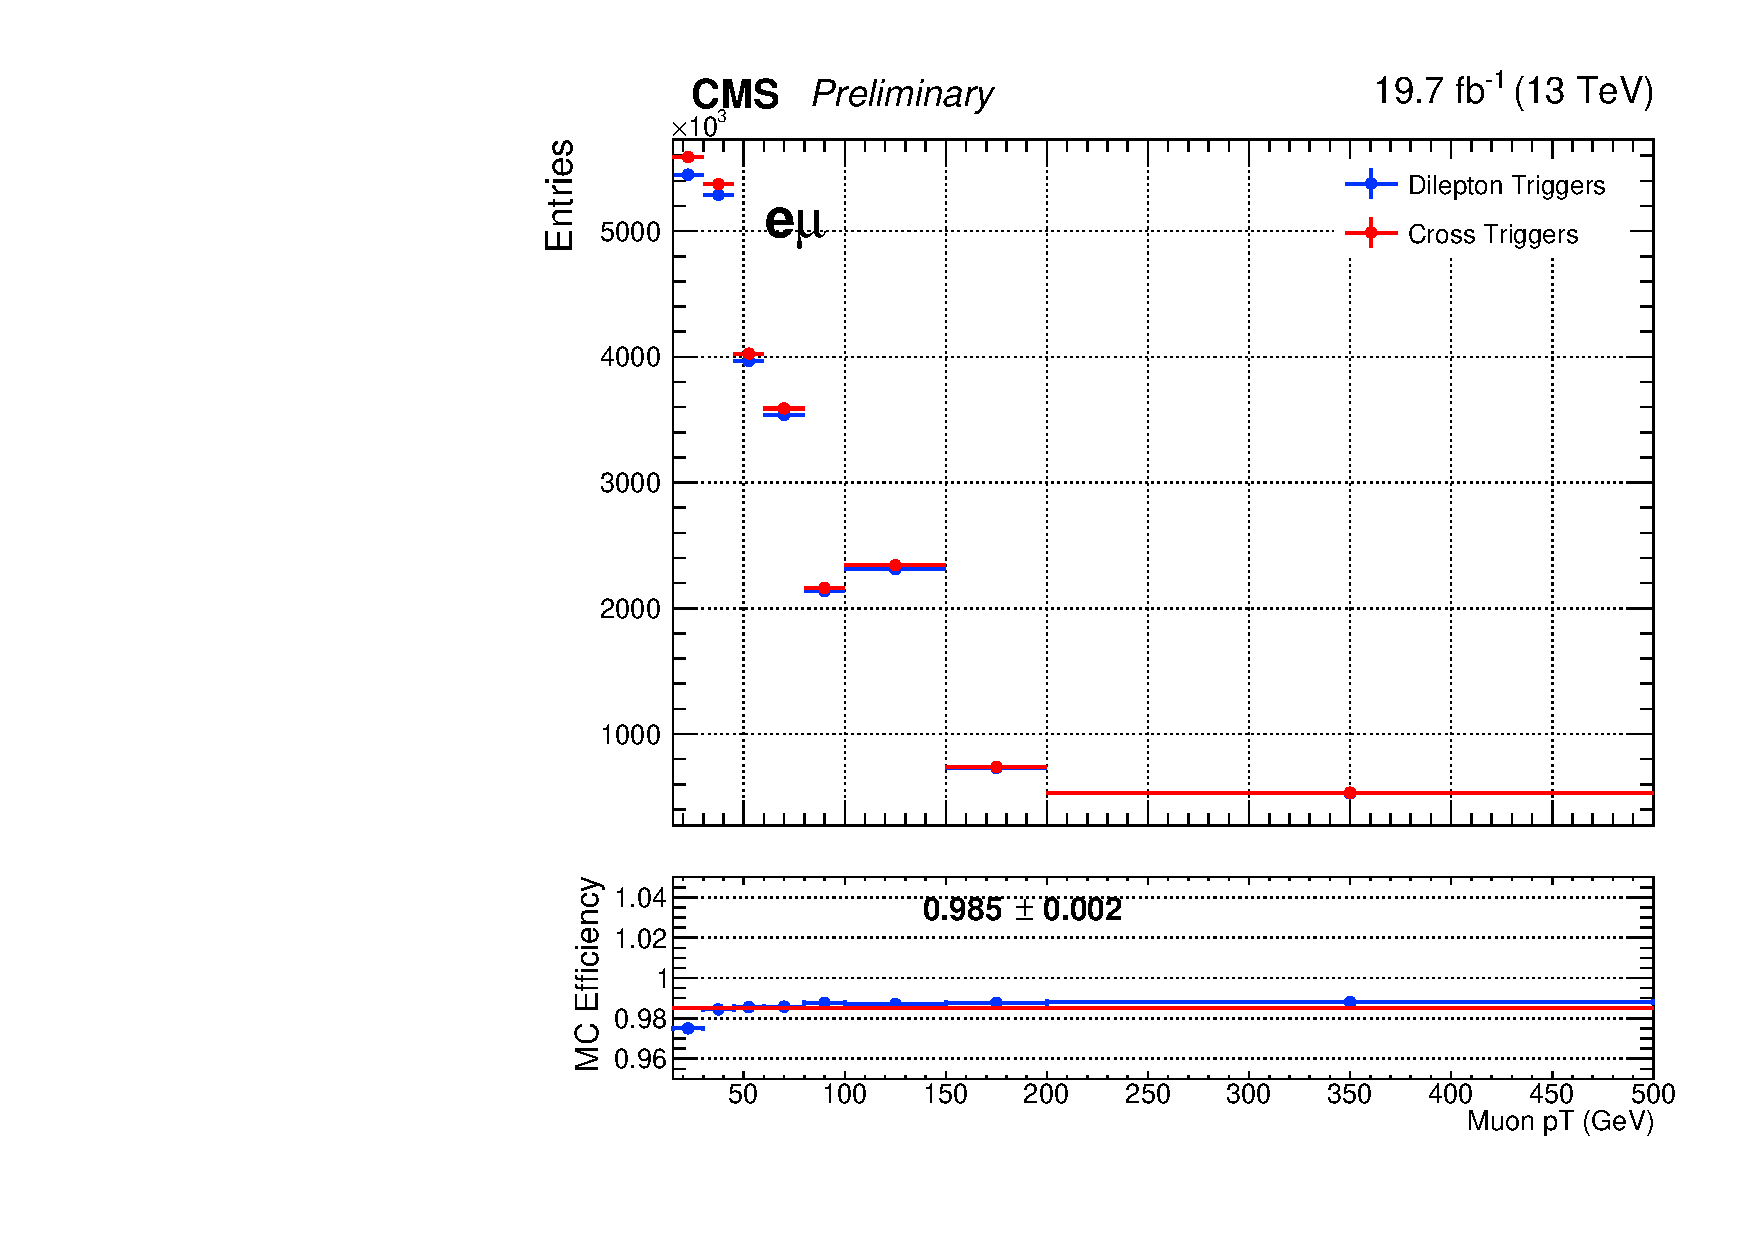
\includegraphics[width=0.32\textwidth]{fig_2016preVFP_TrigSF/g_lepBpt_emu_MC.pdf}
      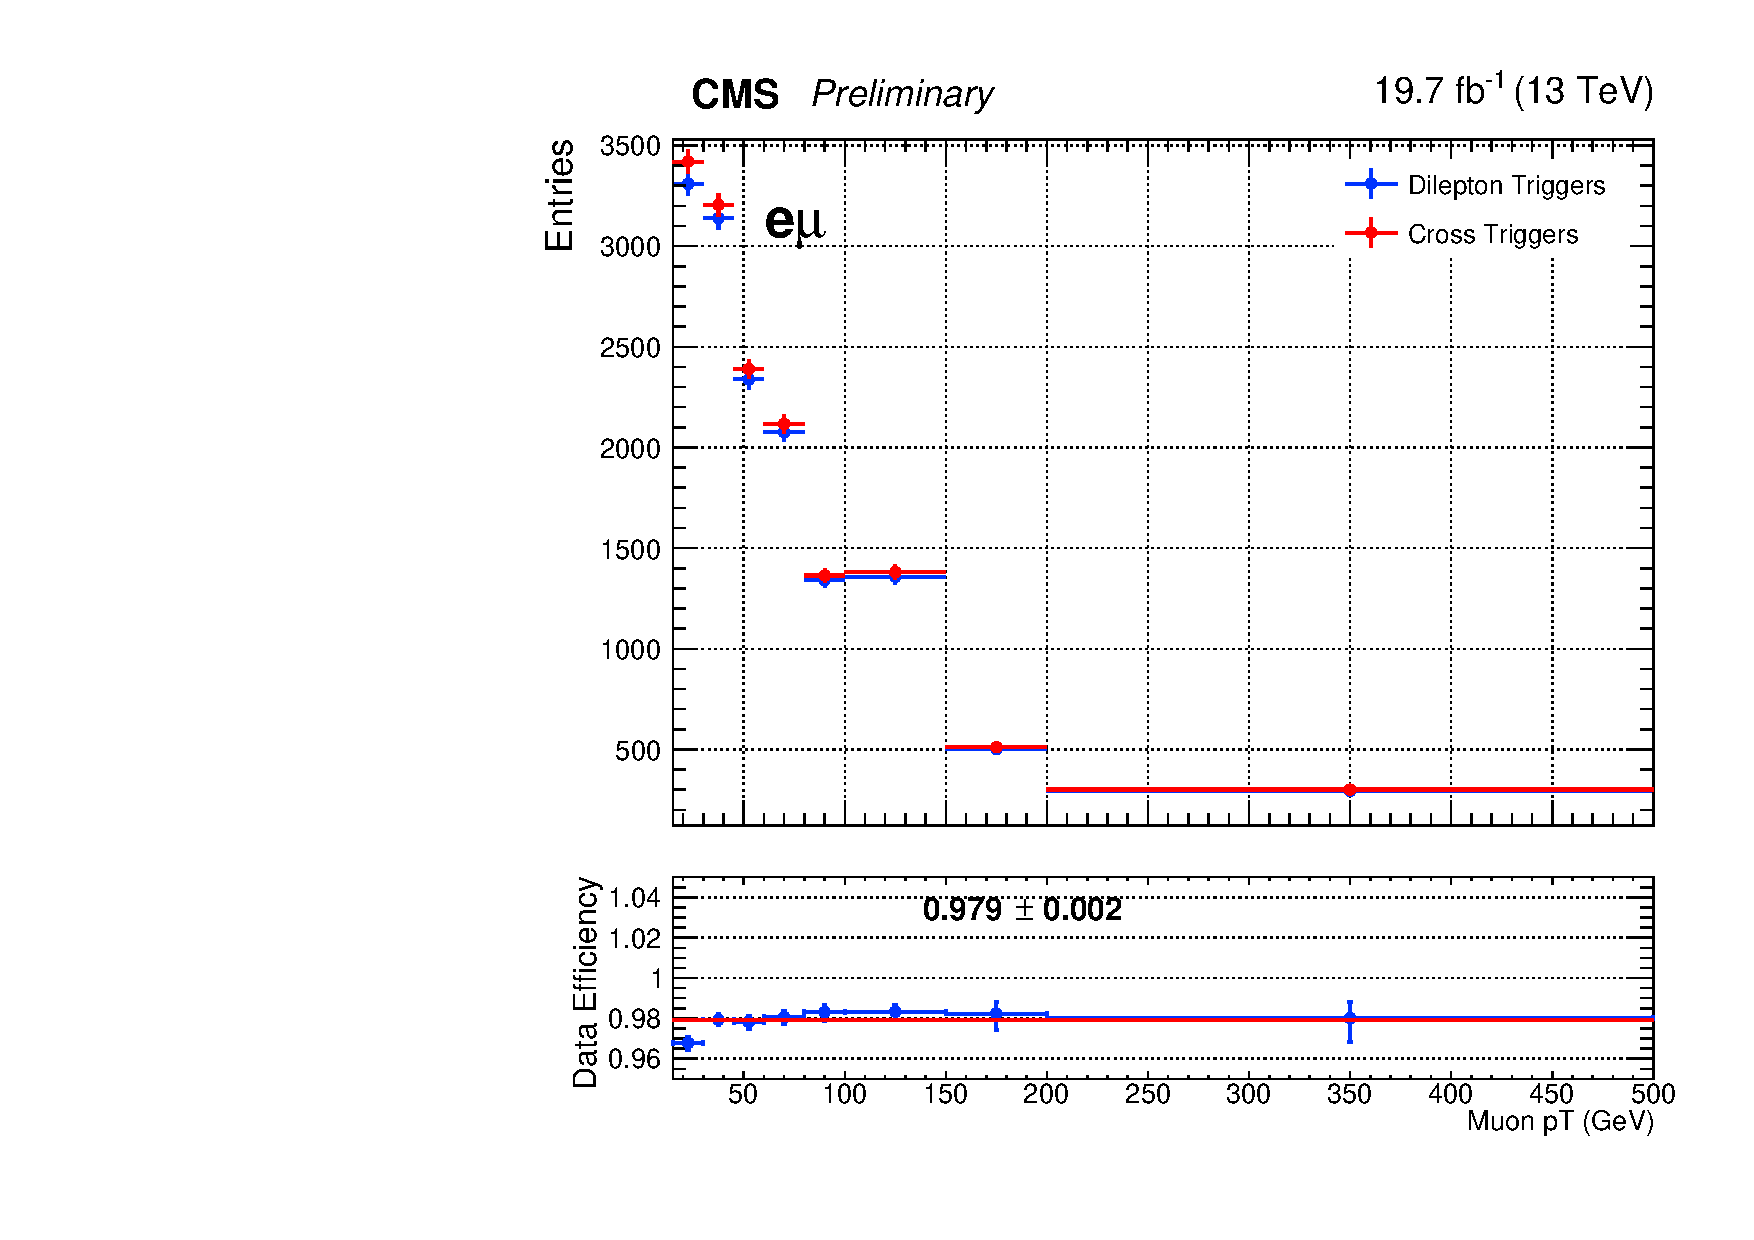
\includegraphics[width=0.32\textwidth]{fig_2016preVFP_TrigSF/g_lepBpt_emu_data.pdf}
      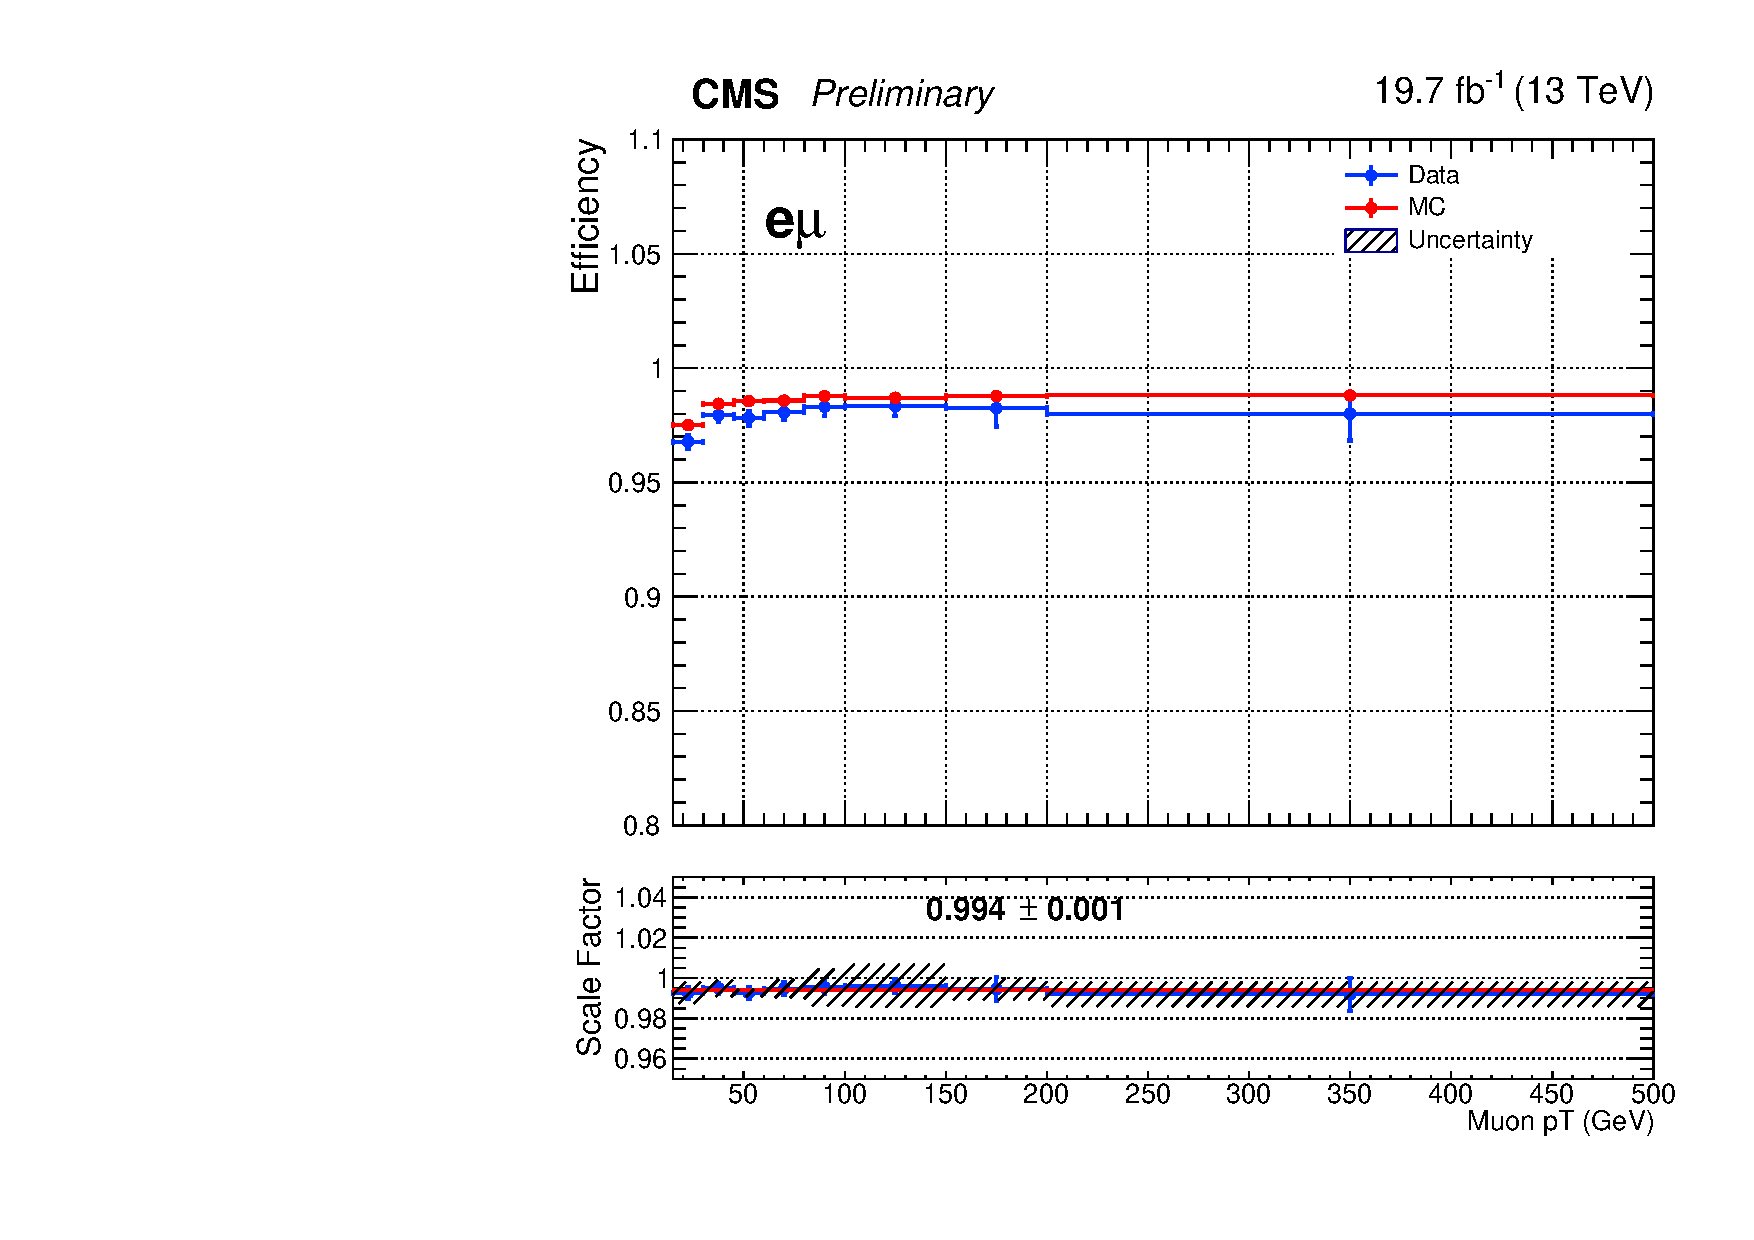
\includegraphics[width=0.32\textwidth]{fig_2016preVFP_TrigSF/g_emu_lepBpt_FullSystUncBand.pdf}\\
    \end{tabular}
    \caption{Efficiencies and scale factors for the 2016preVFP data set in the \emu channel as a function of electron and muon \pT.
            The error bars indicate the statistical uncertainty, and the shaded band corresponds to the systematic uncertainty.
            }
    \label{TrigSF_2016preVFP_1}
  \end{center}
\end{figure}

\begin{figure}[h]
  \begin{center}
    \begin{tabular}{ccc}
      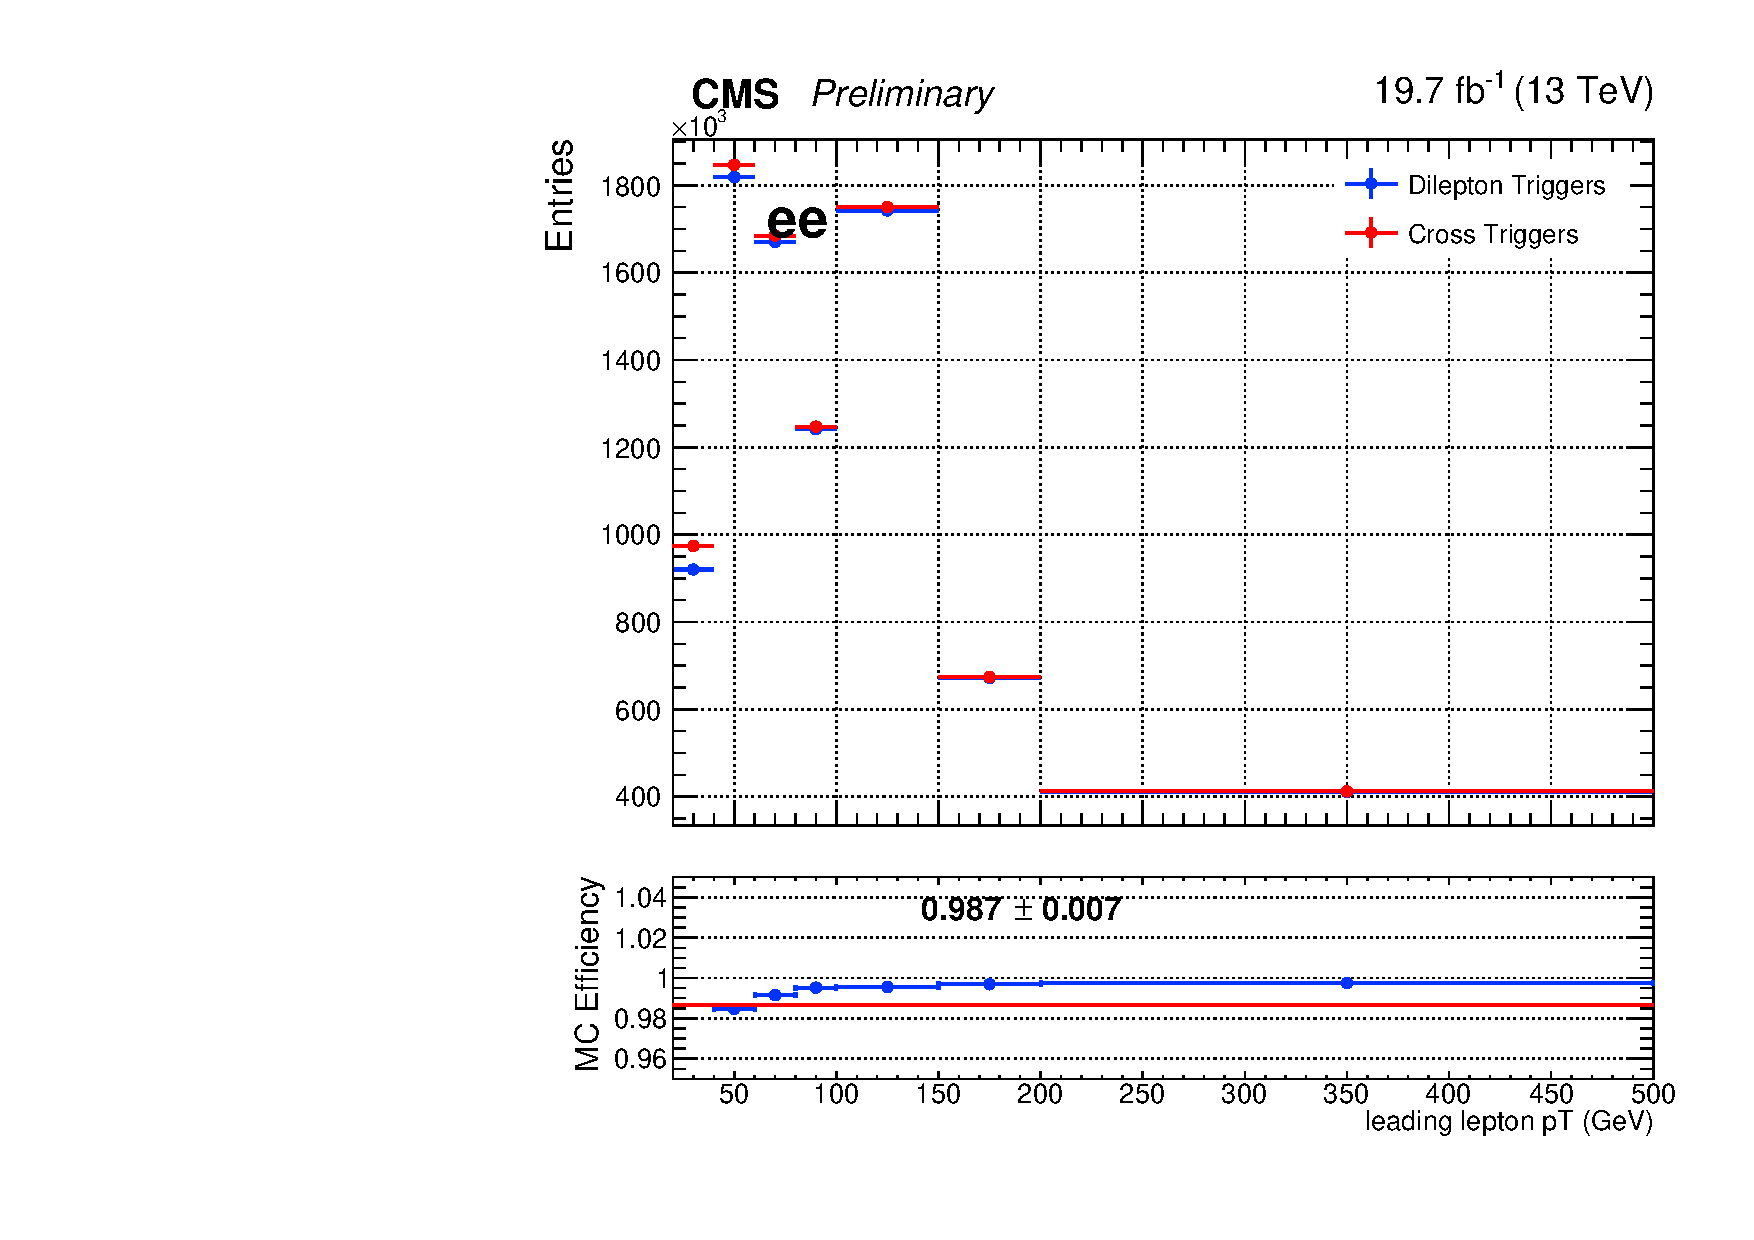
\includegraphics[width=0.32\textwidth]{fig_2016preVFP_TrigSF/g_lepApt_ee_MC.pdf}
      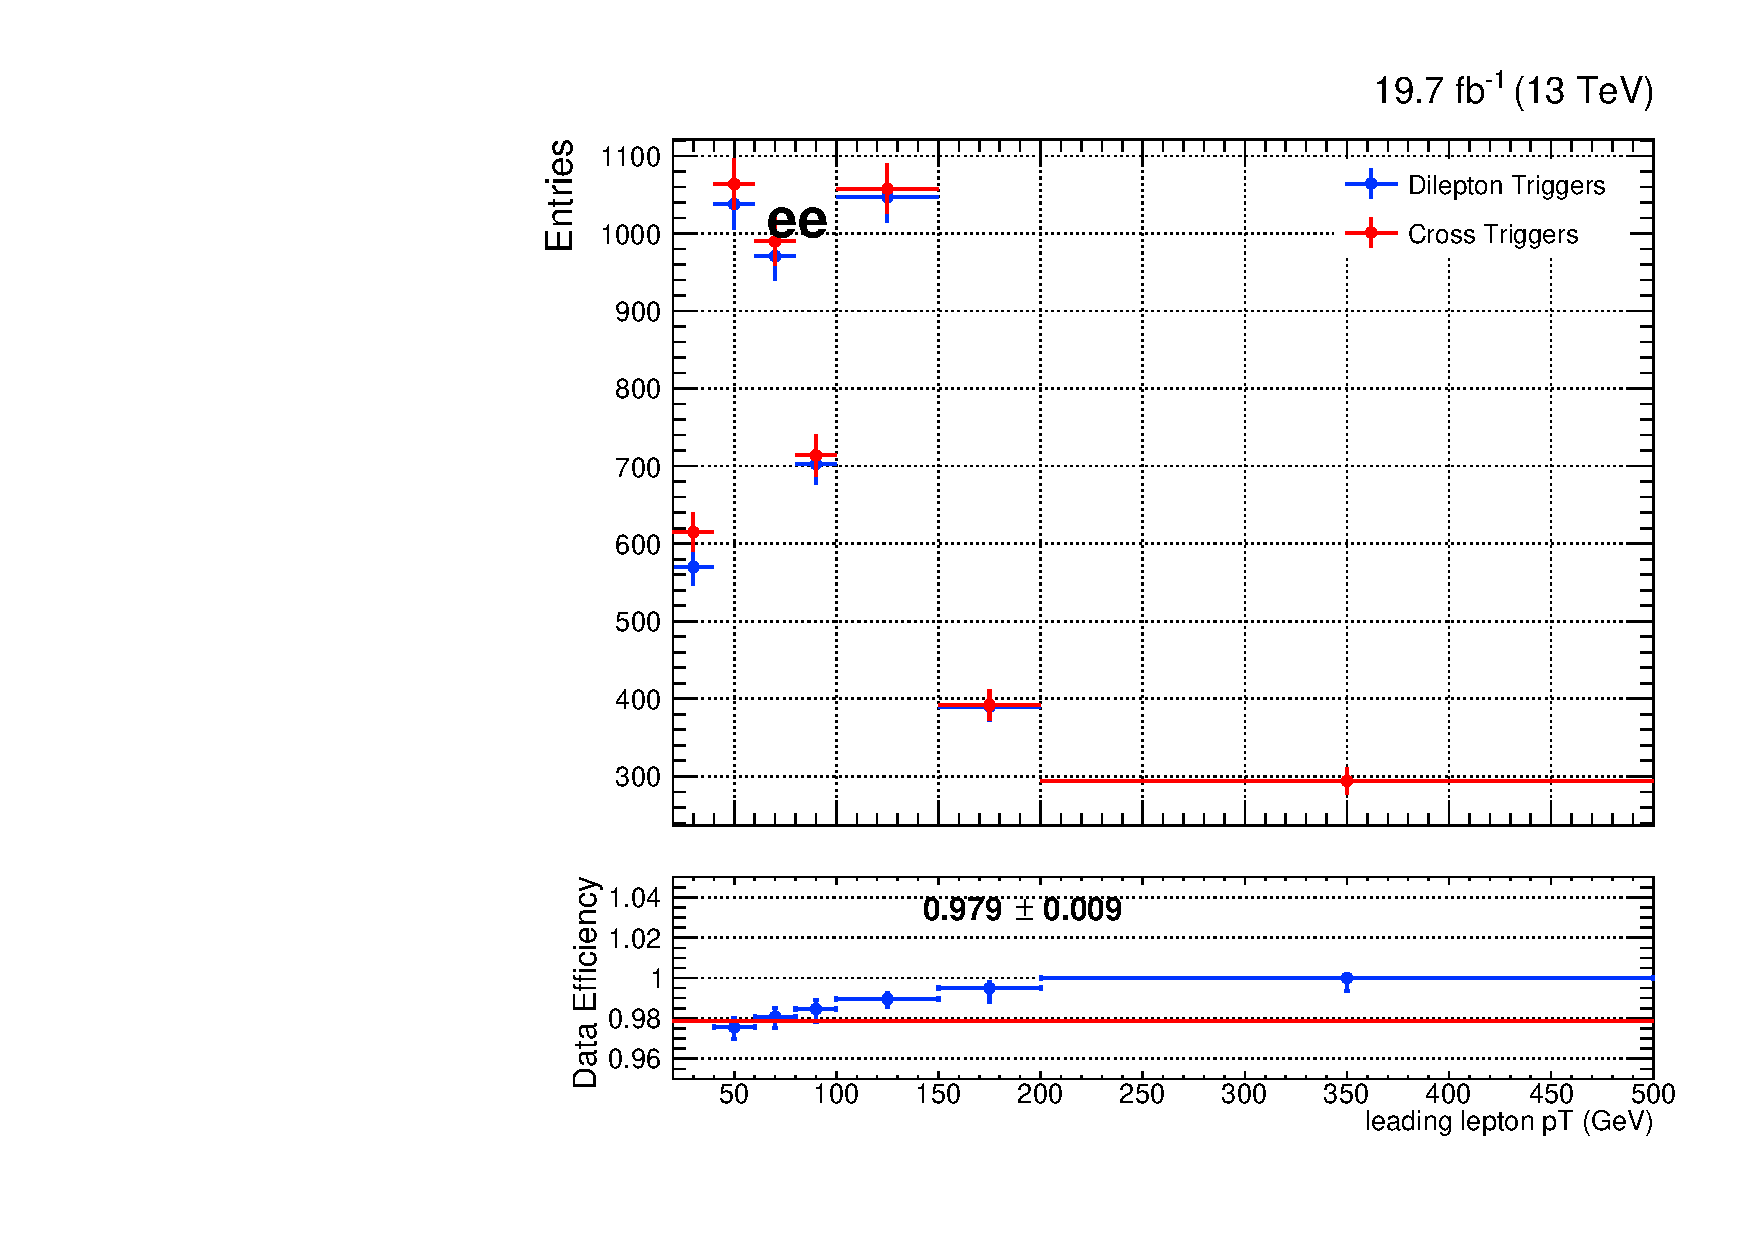
\includegraphics[width=0.32\textwidth]{fig_2016preVFP_TrigSF/g_lepApt_ee_data.pdf}
      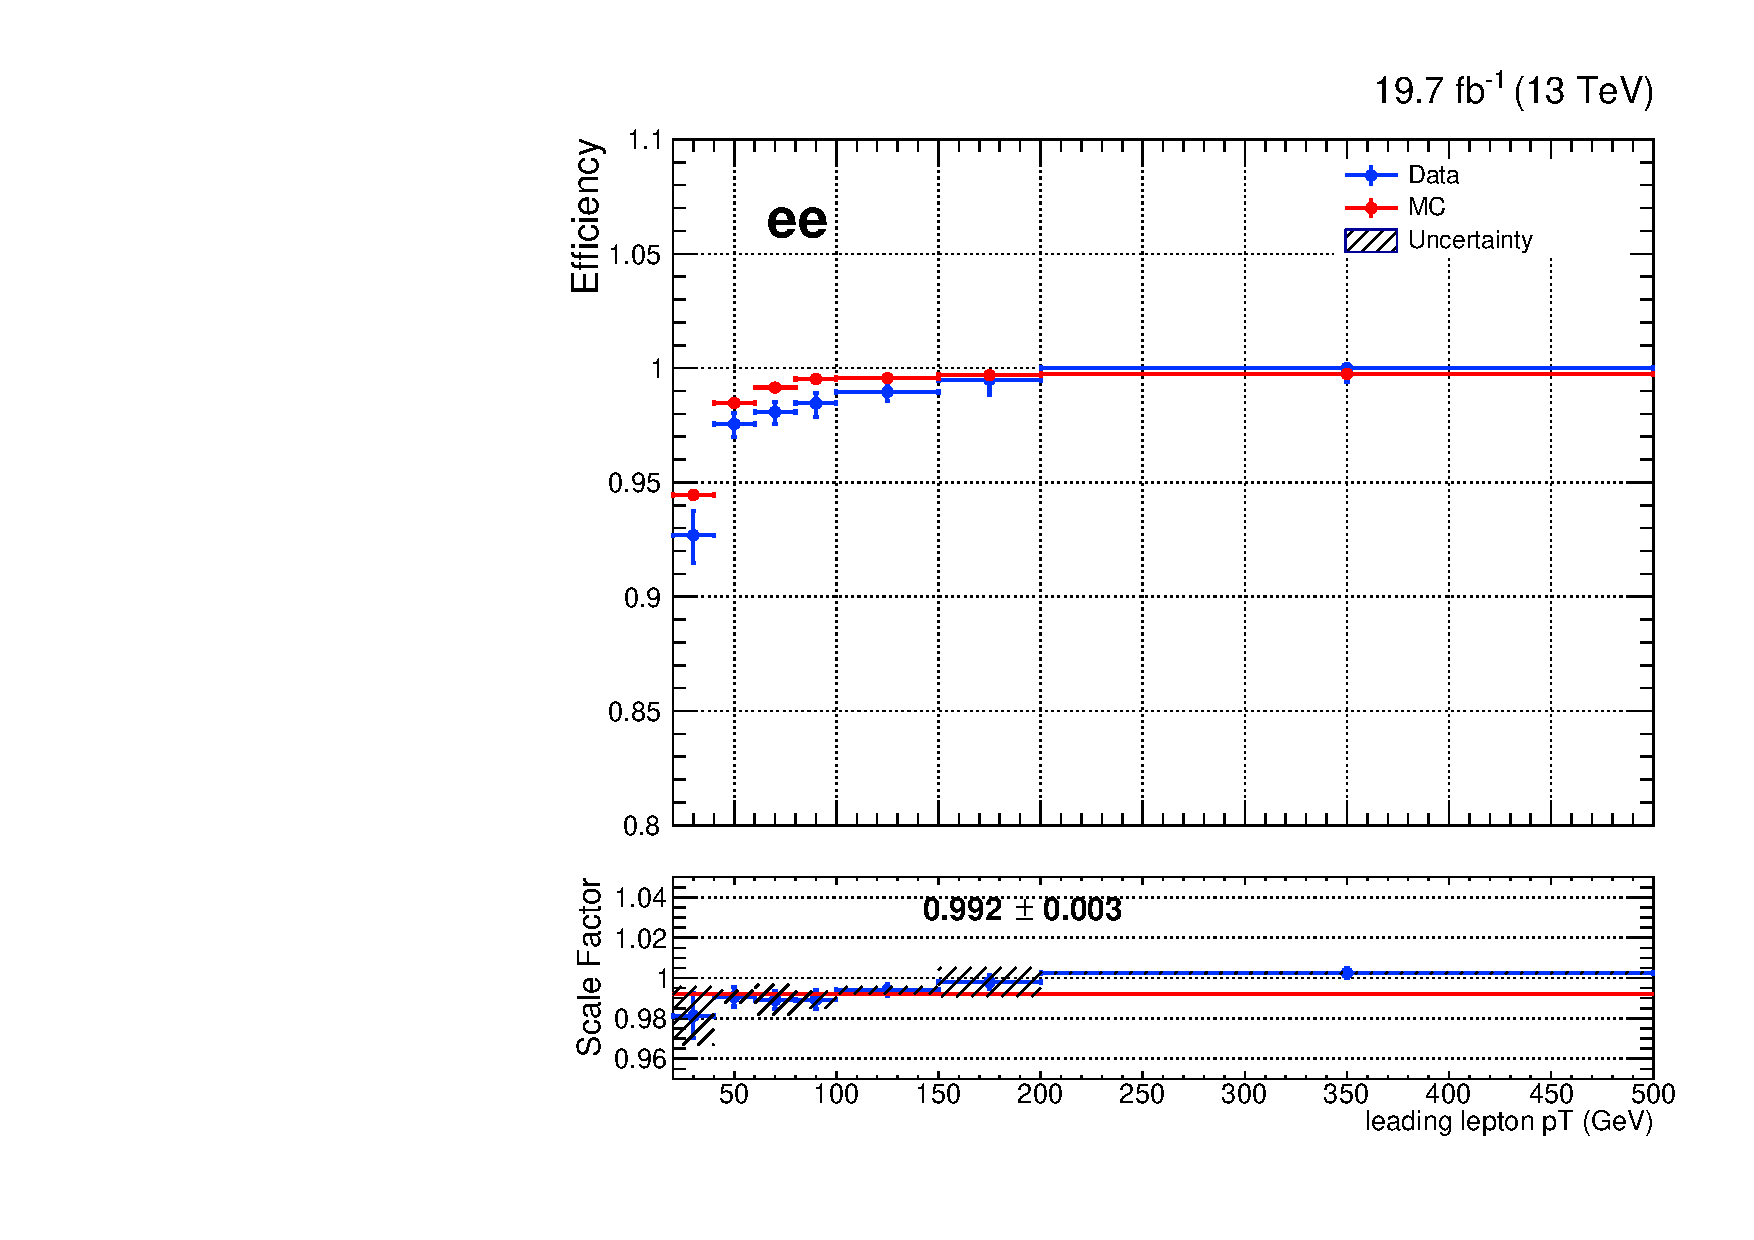
\includegraphics[width=0.32\textwidth]{fig_2016preVFP_TrigSF/g_ee_lepApt_FullSystUncBand.pdf}\\
      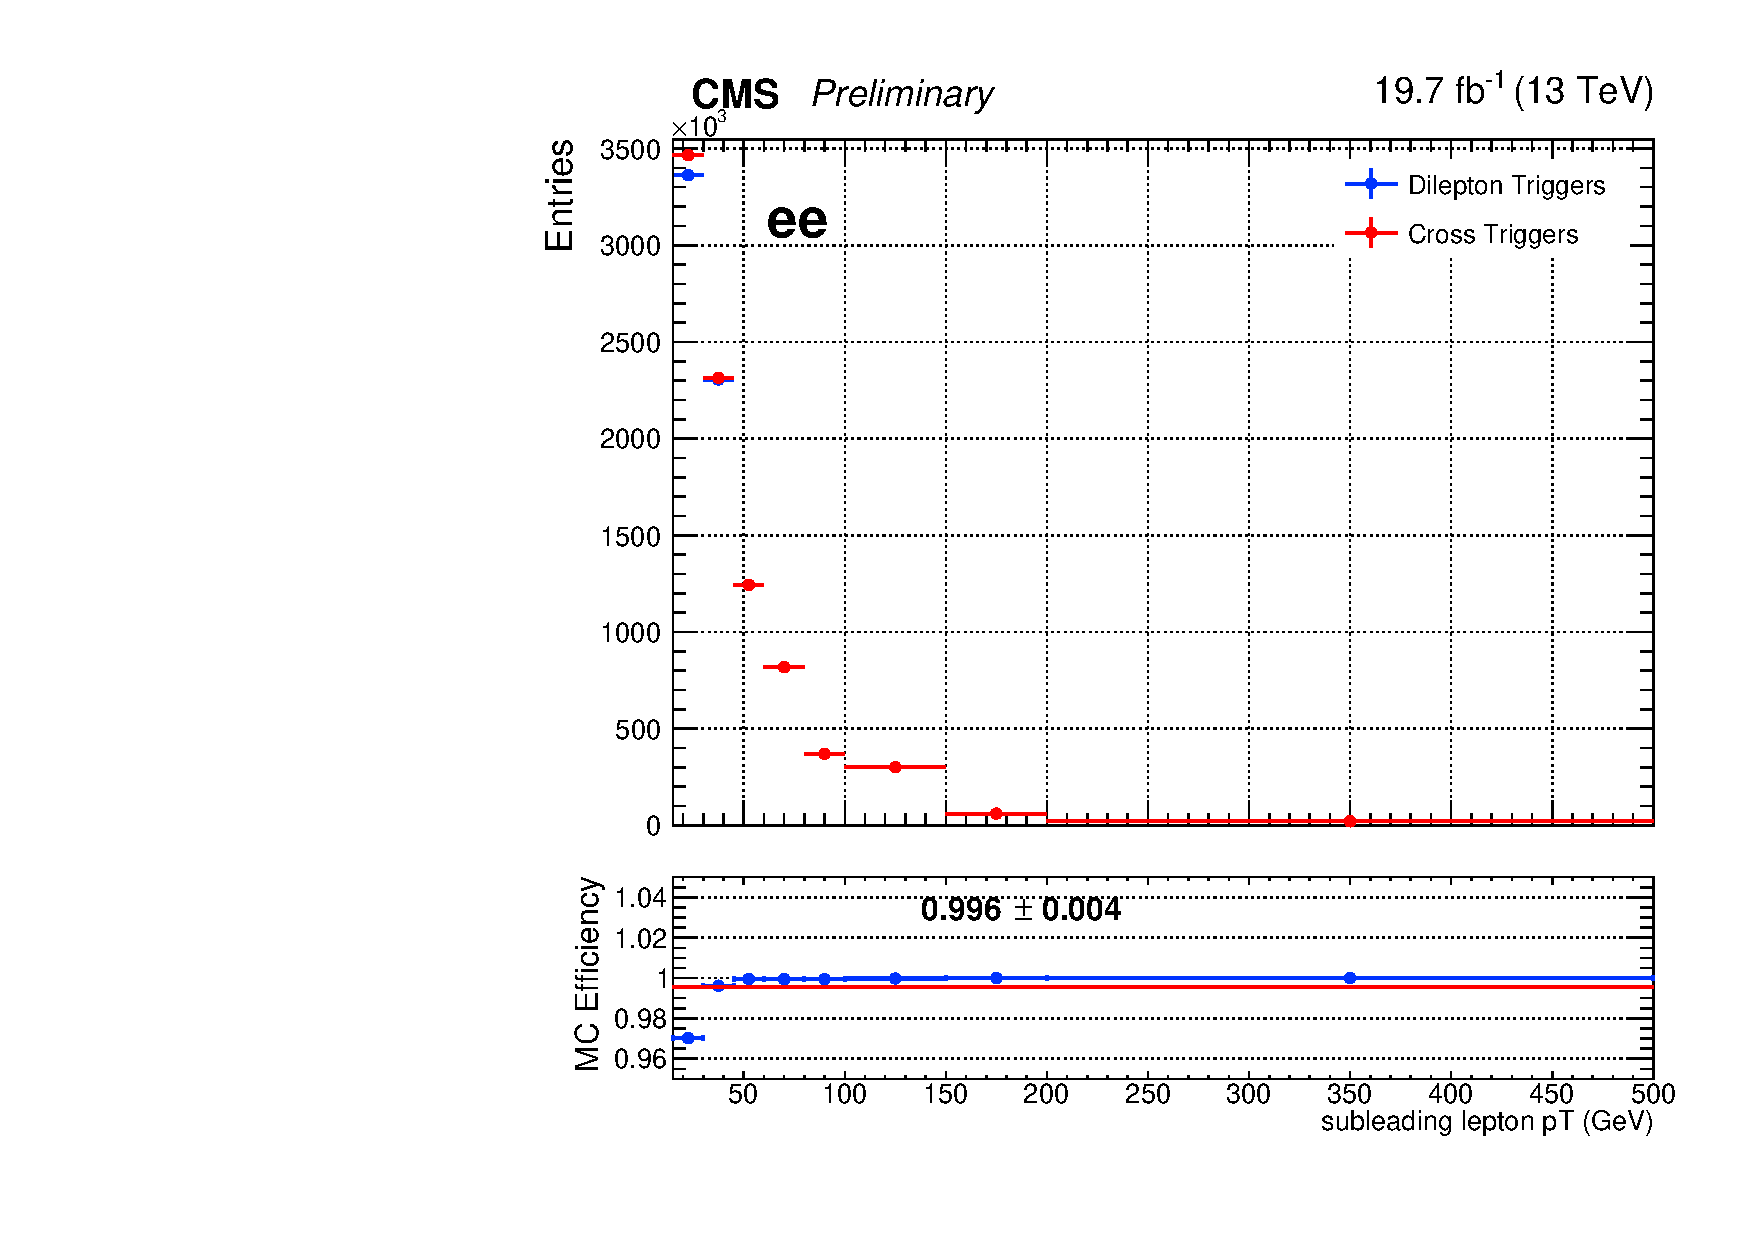
\includegraphics[width=0.32\textwidth]{fig_2016preVFP_TrigSF/g_lepBpt_ee_MC.pdf}
      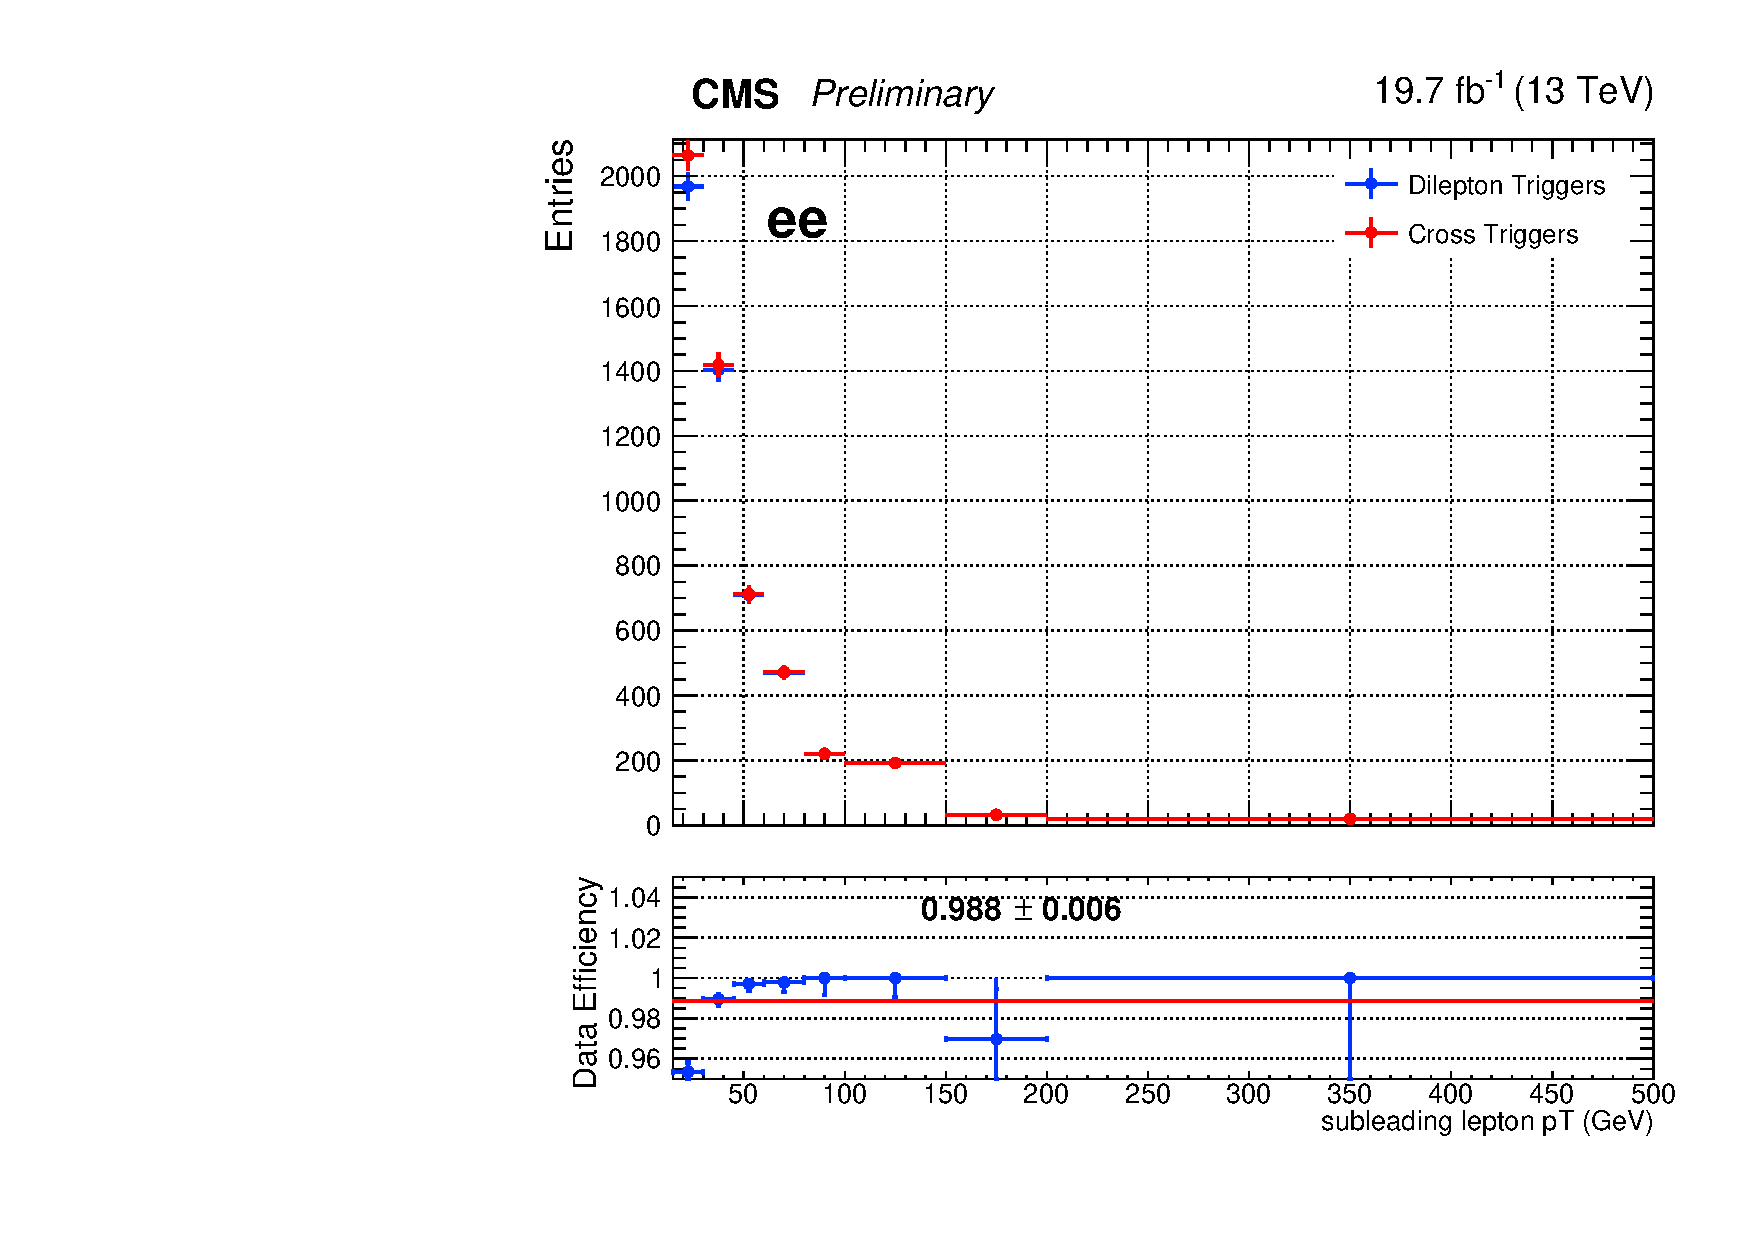
\includegraphics[width=0.32\textwidth]{fig_2016preVFP_TrigSF/g_lepBpt_ee_data.pdf}
      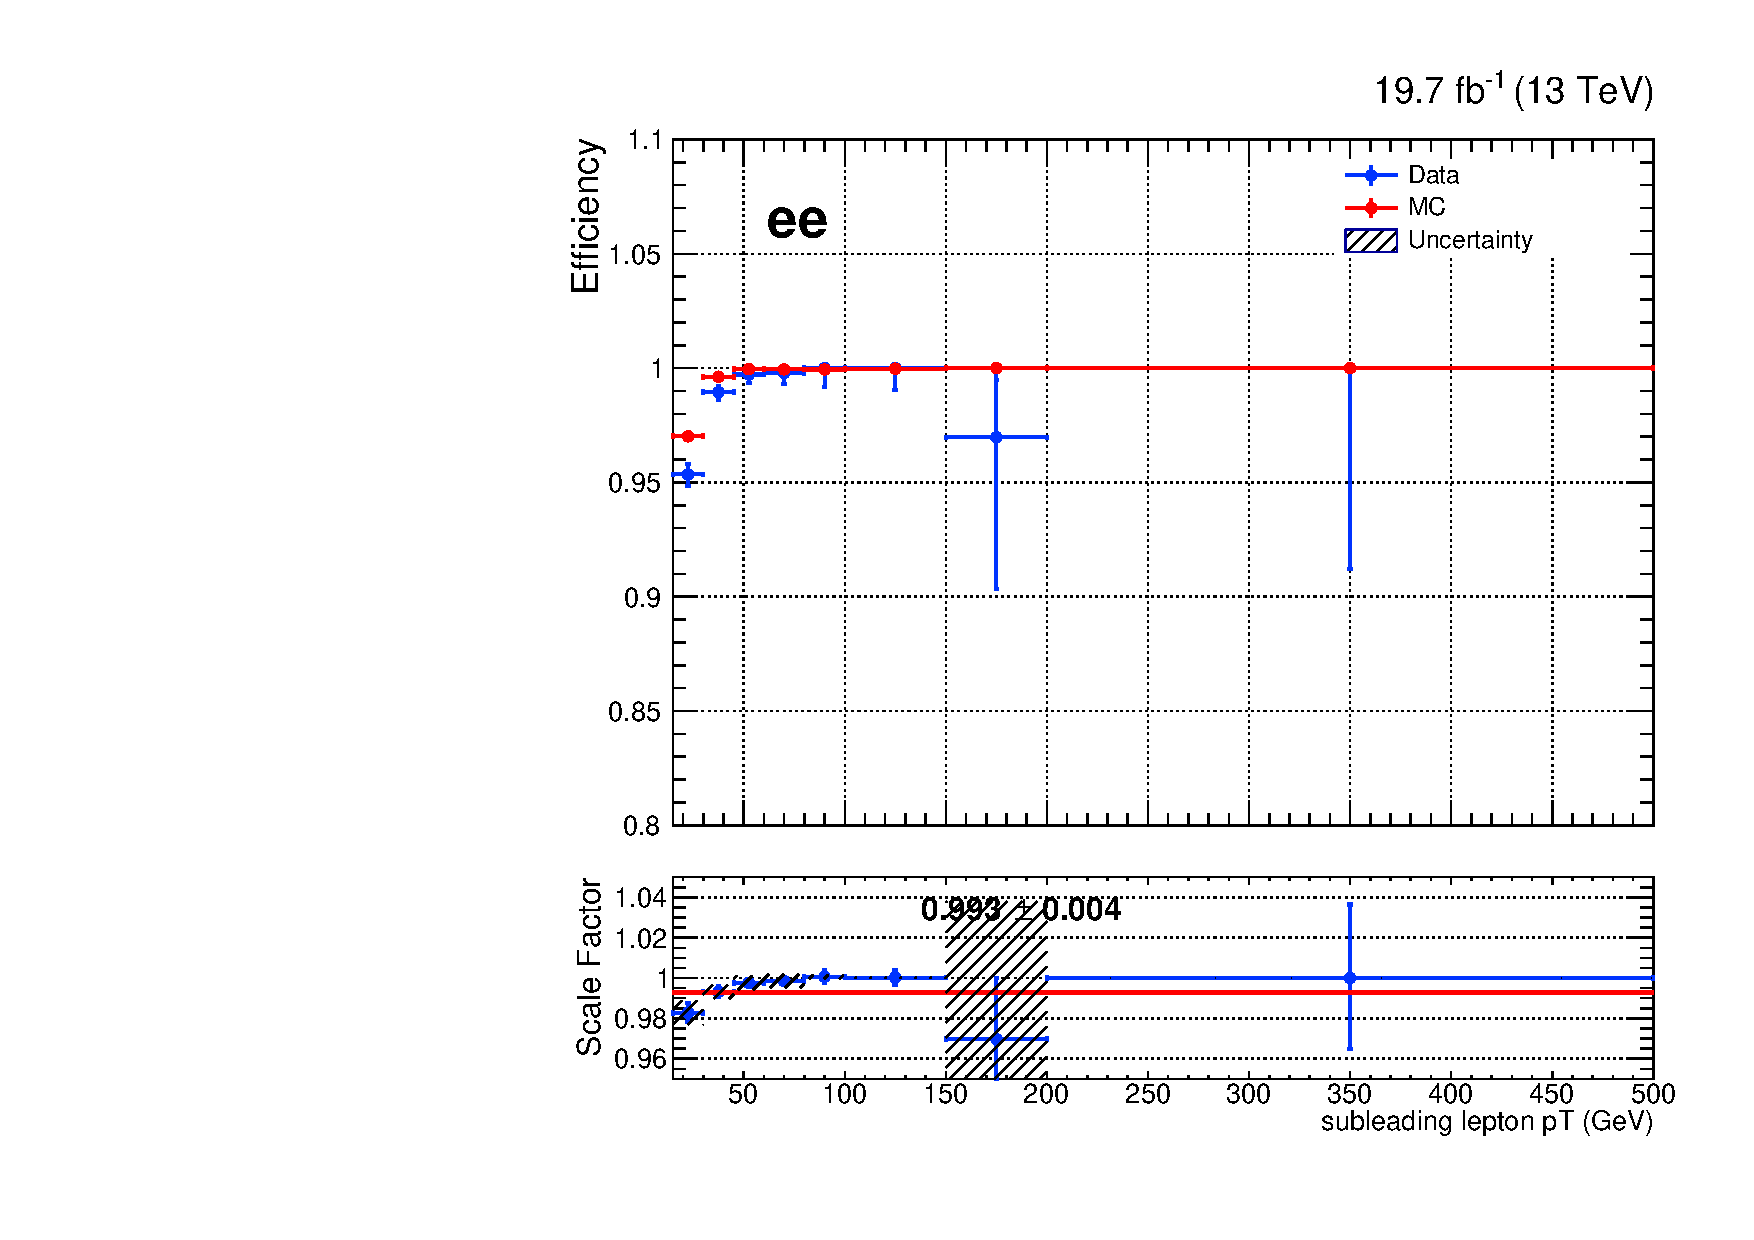
\includegraphics[width=0.32\textwidth]{fig_2016preVFP_TrigSF/g_ee_lepBpt_FullSystUncBand.pdf}\\
    \end{tabular}
    \caption{Efficiencies and scale factors for the 2016preVFP data set in the \ee channel as a function of leading and sub-leading lepton \pT.
            The error bars indicate the statistical uncertainty, and the shaded band corresponds to the systematic uncertainty.
            }
    \label{TrigSF_2016preVFP_2}
  \end{center}
\end{figure}

\begin{figure}[h]
  \begin{center}
    \begin{tabular}{ccc}
      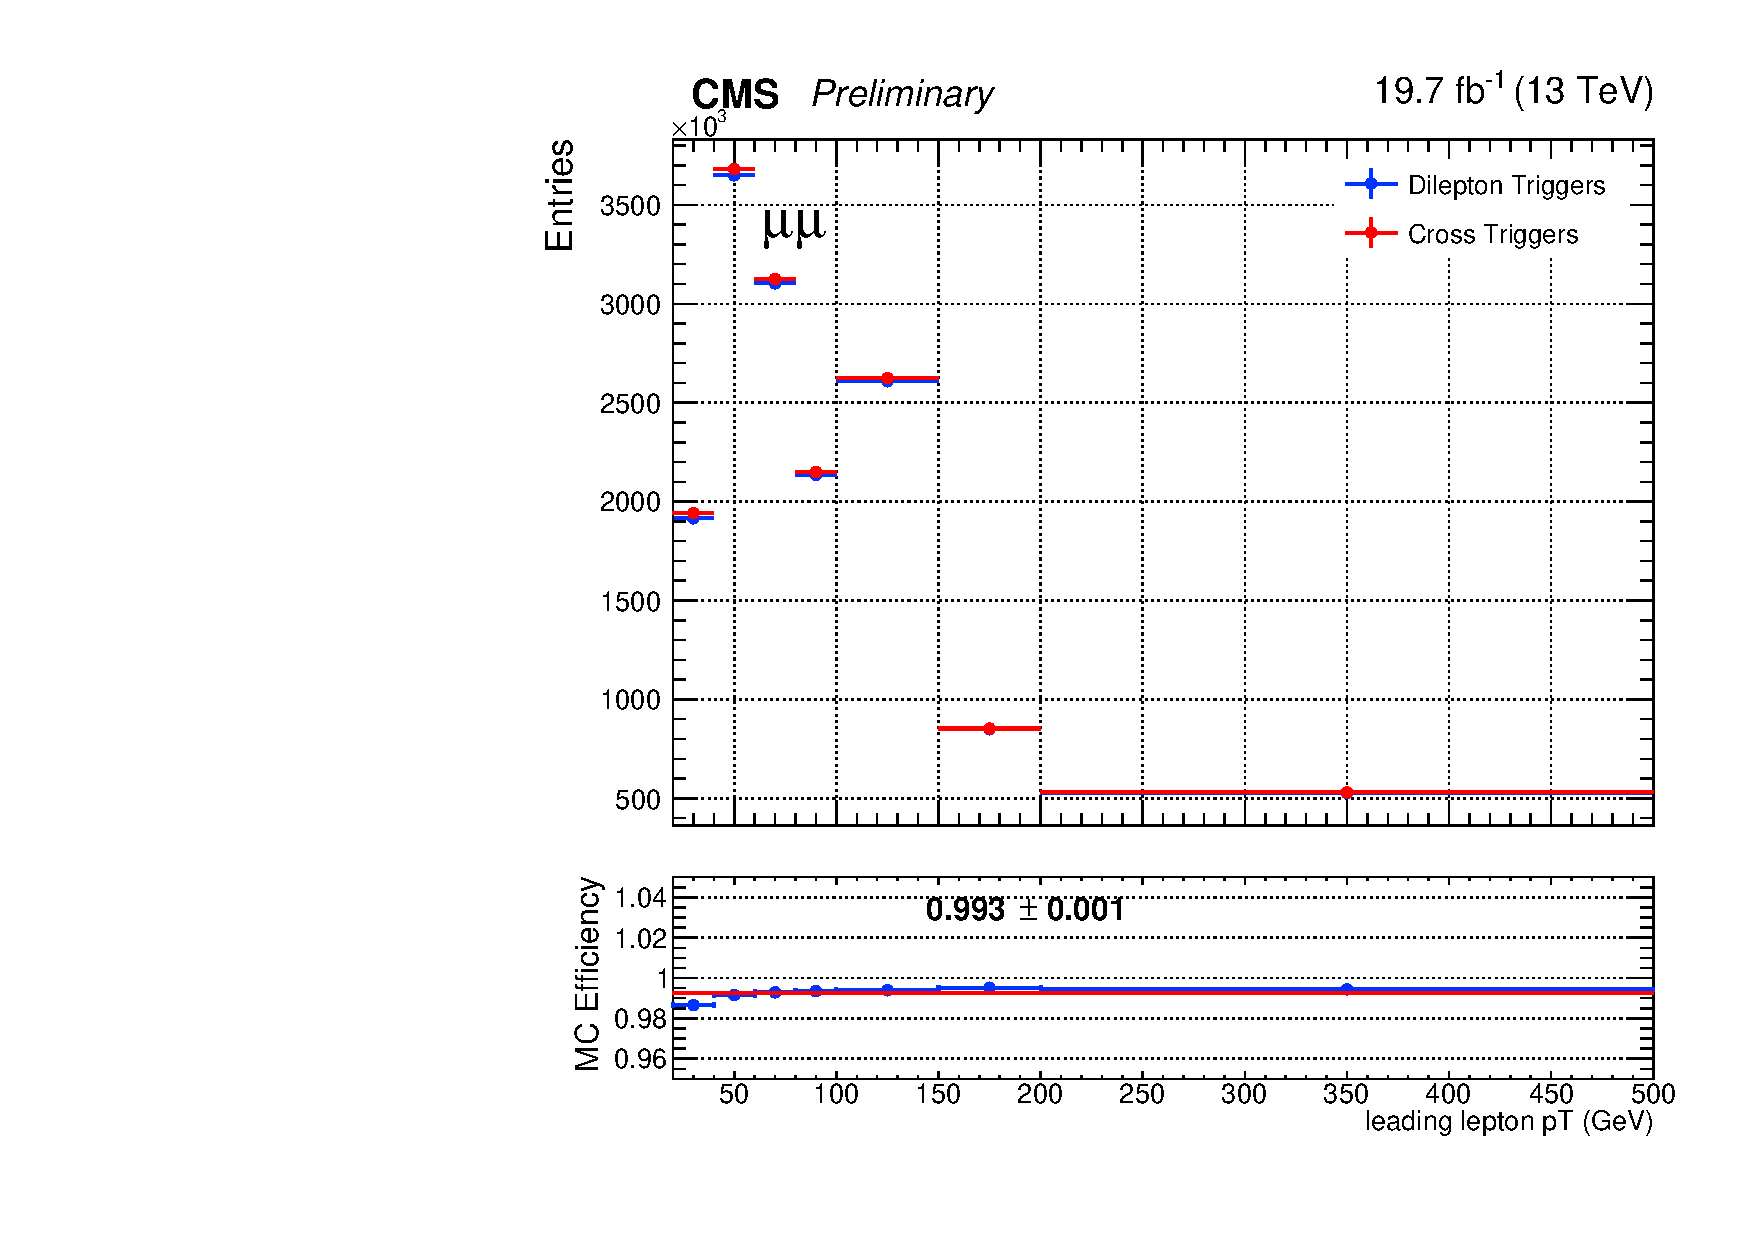
\includegraphics[width=0.32\textwidth]{fig_2016preVFP_TrigSF/g_lepApt_mumu_MC.pdf}
      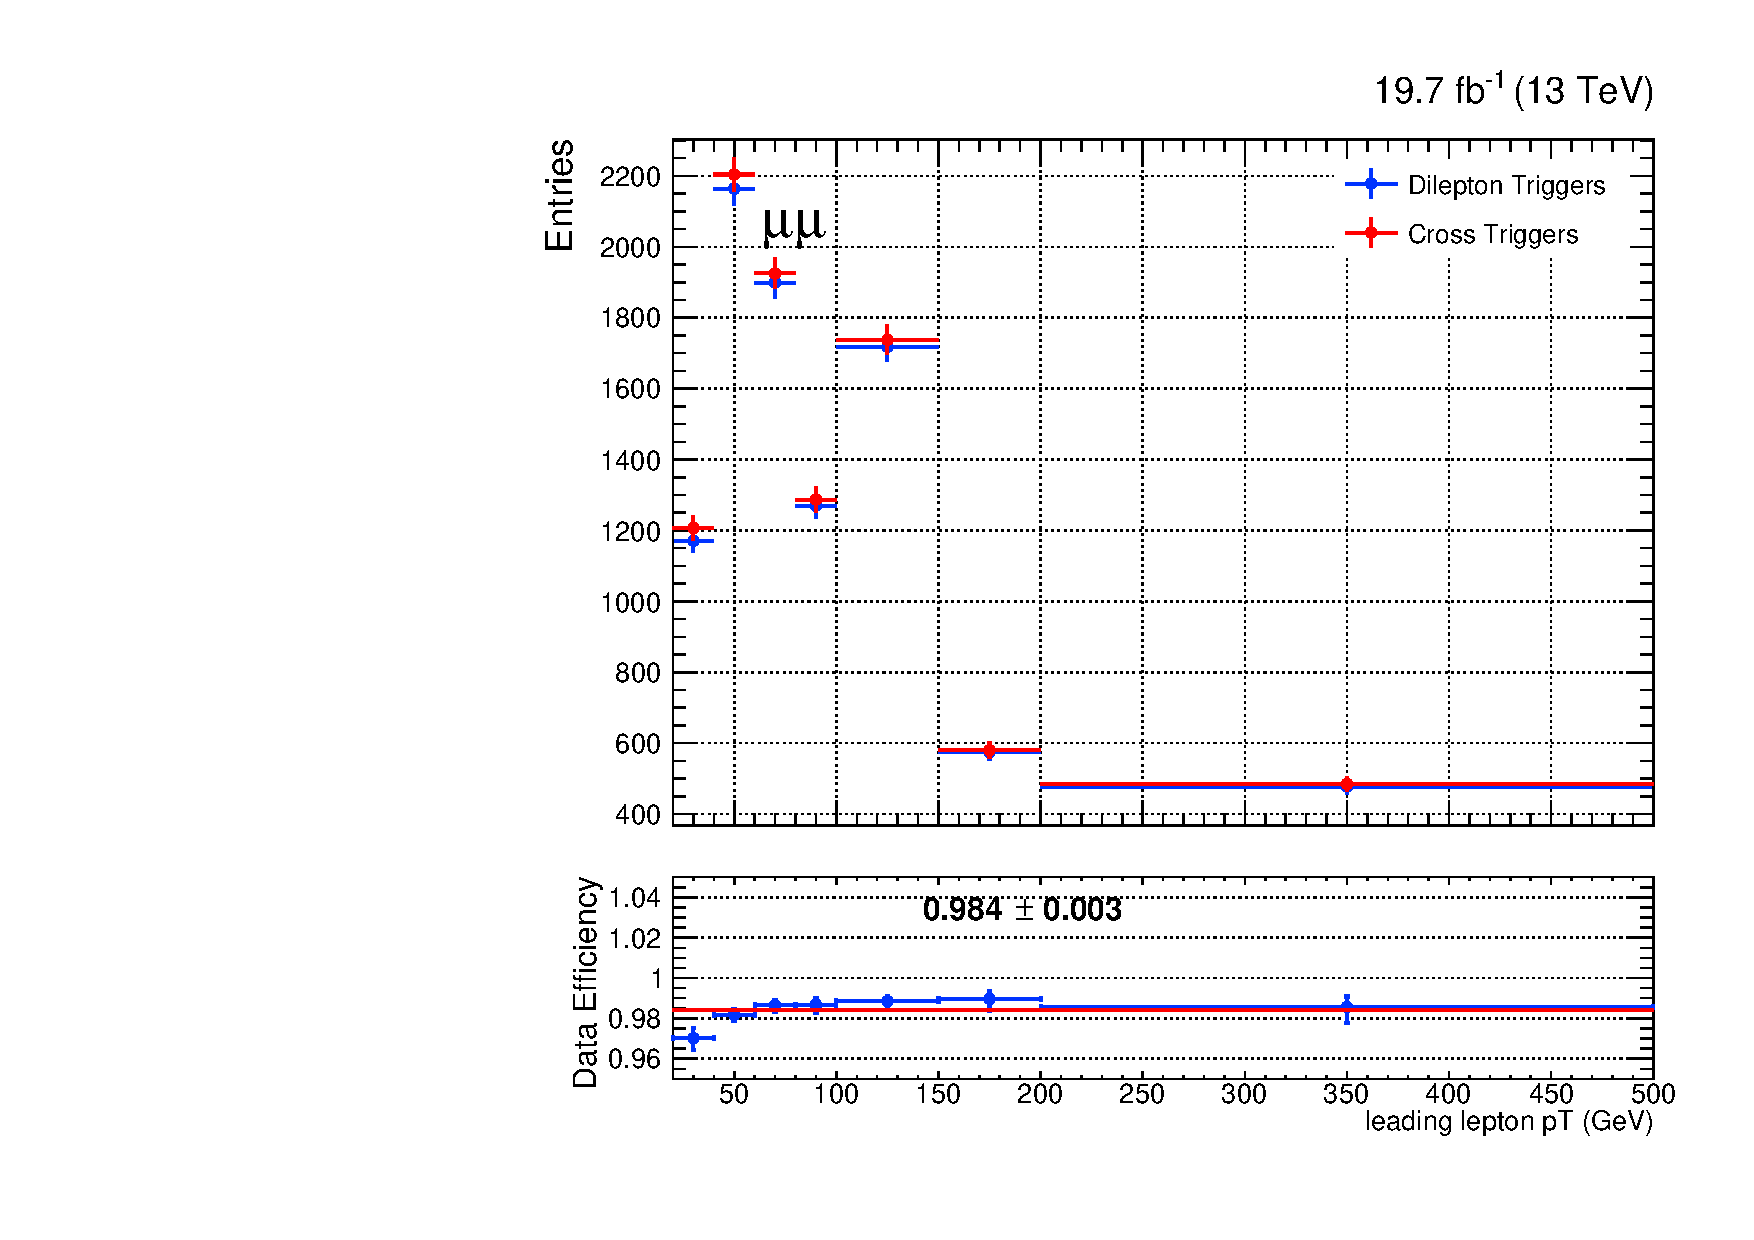
\includegraphics[width=0.32\textwidth]{fig_2016preVFP_TrigSF/g_lepApt_mumu_data.pdf}
      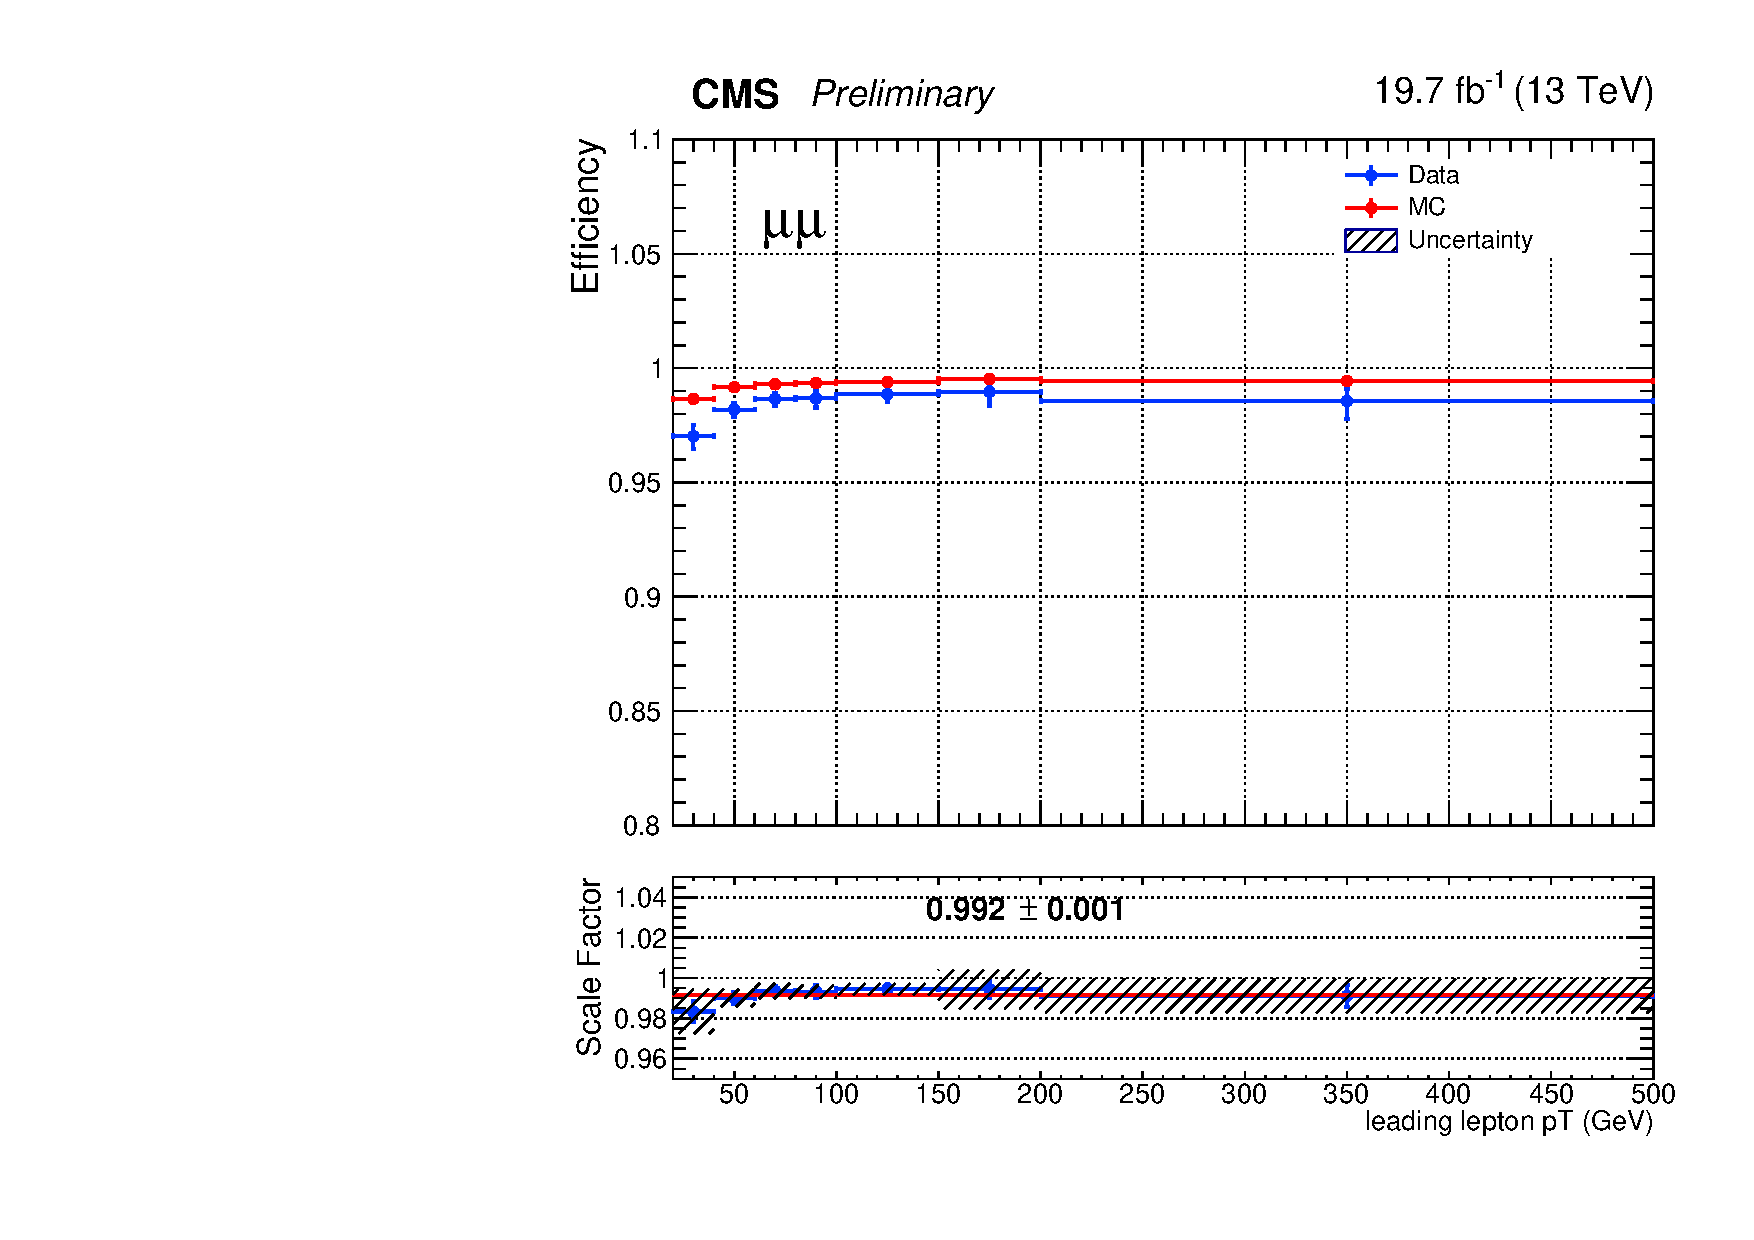
\includegraphics[width=0.32\textwidth]{fig_2016preVFP_TrigSF/g_mumu_lepApt_FullSystUncBand.pdf}\\
      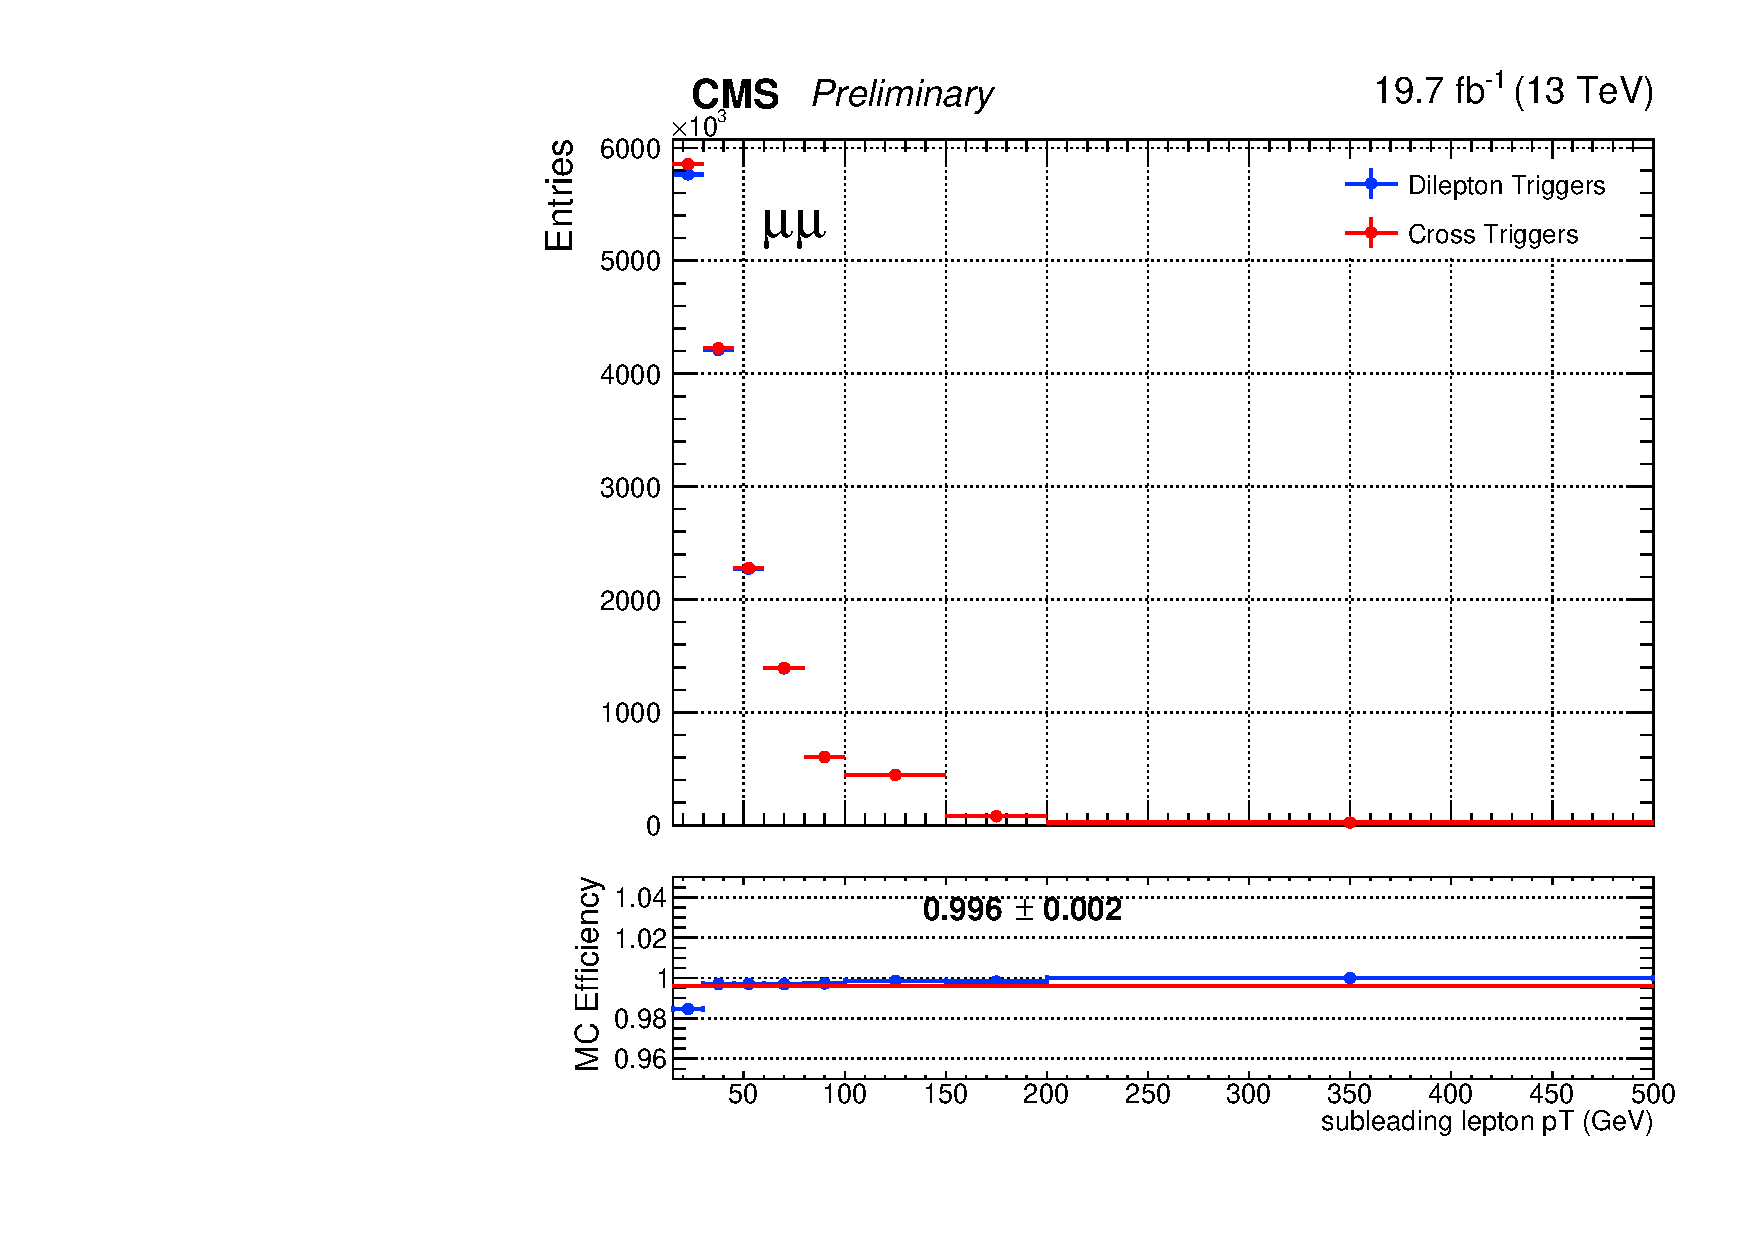
\includegraphics[width=0.32\textwidth]{fig_2016preVFP_TrigSF/g_lepBpt_mumu_MC.pdf}
      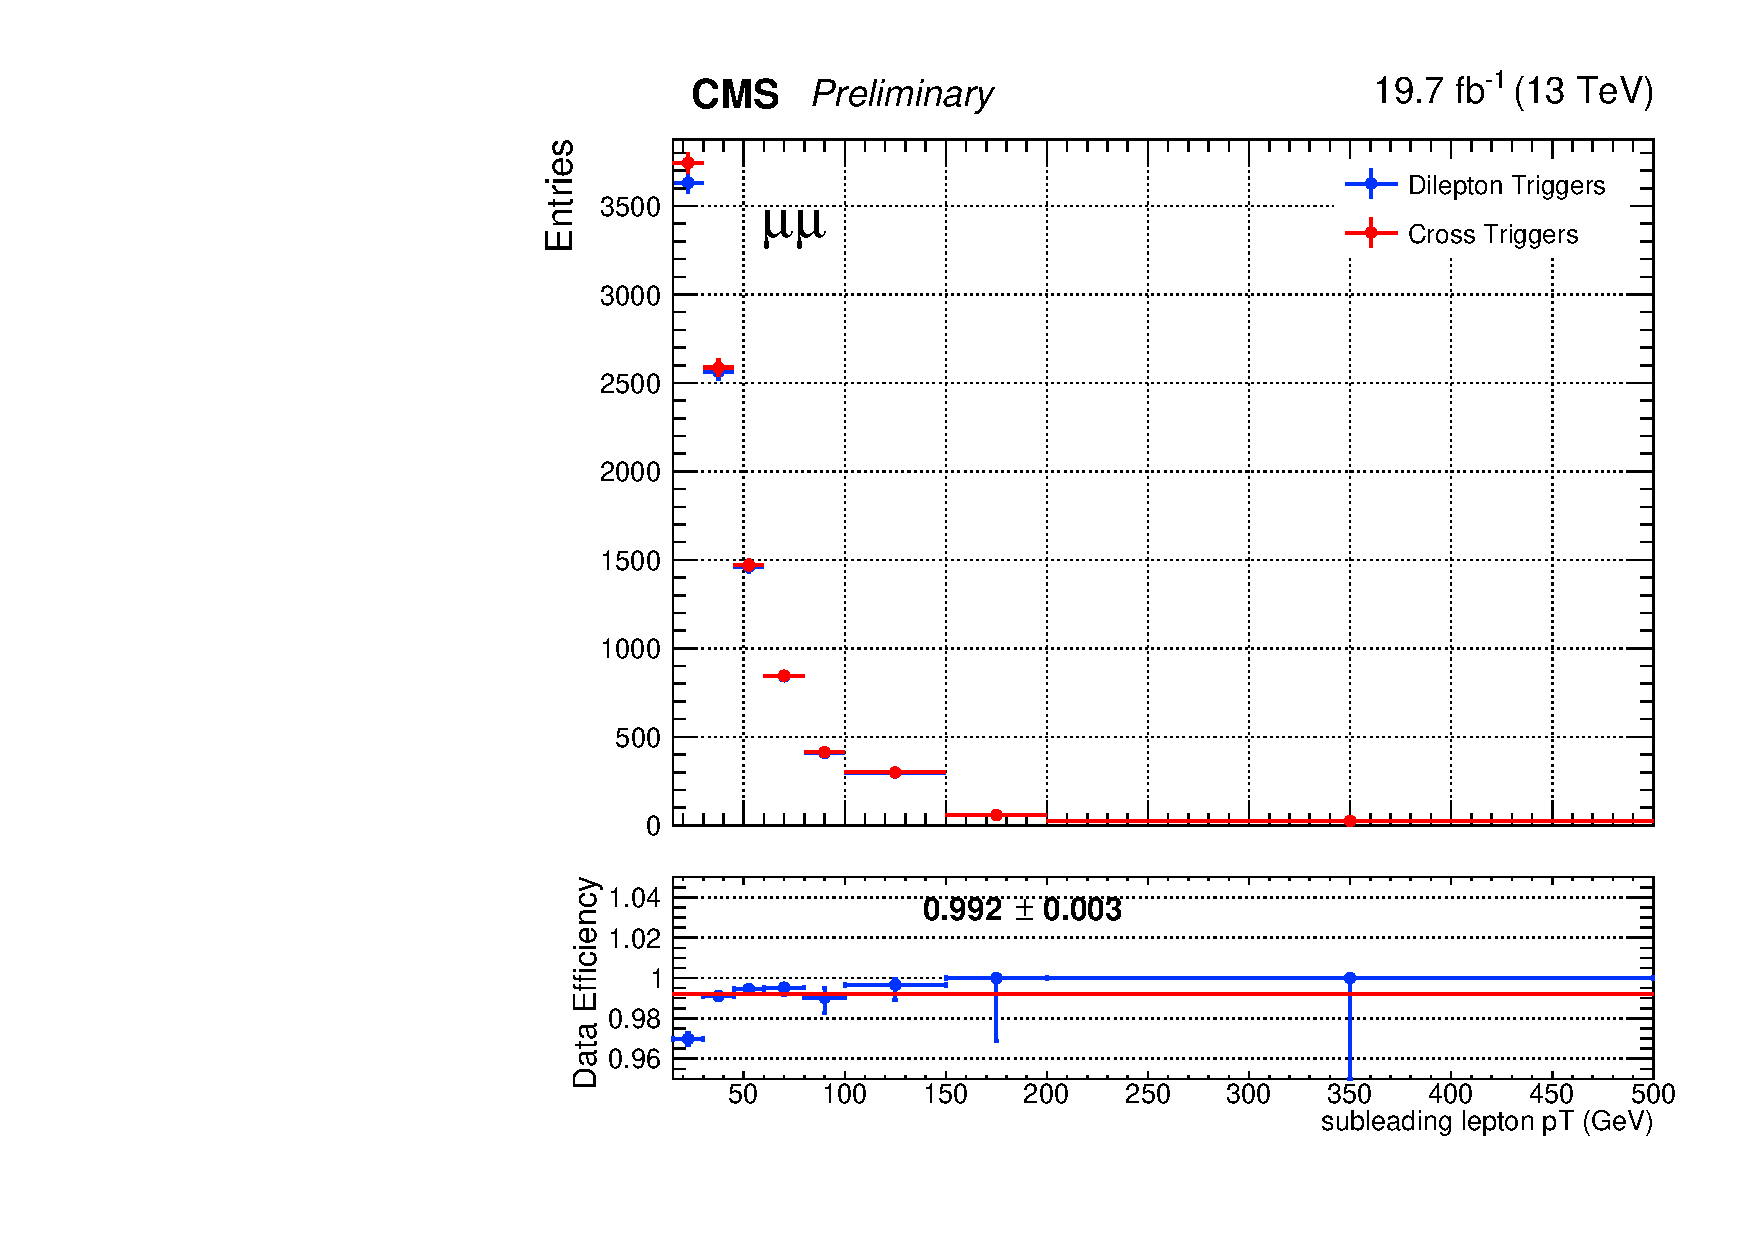
\includegraphics[width=0.32\textwidth]{fig_2016preVFP_TrigSF/g_lepBpt_mumu_data.pdf}
      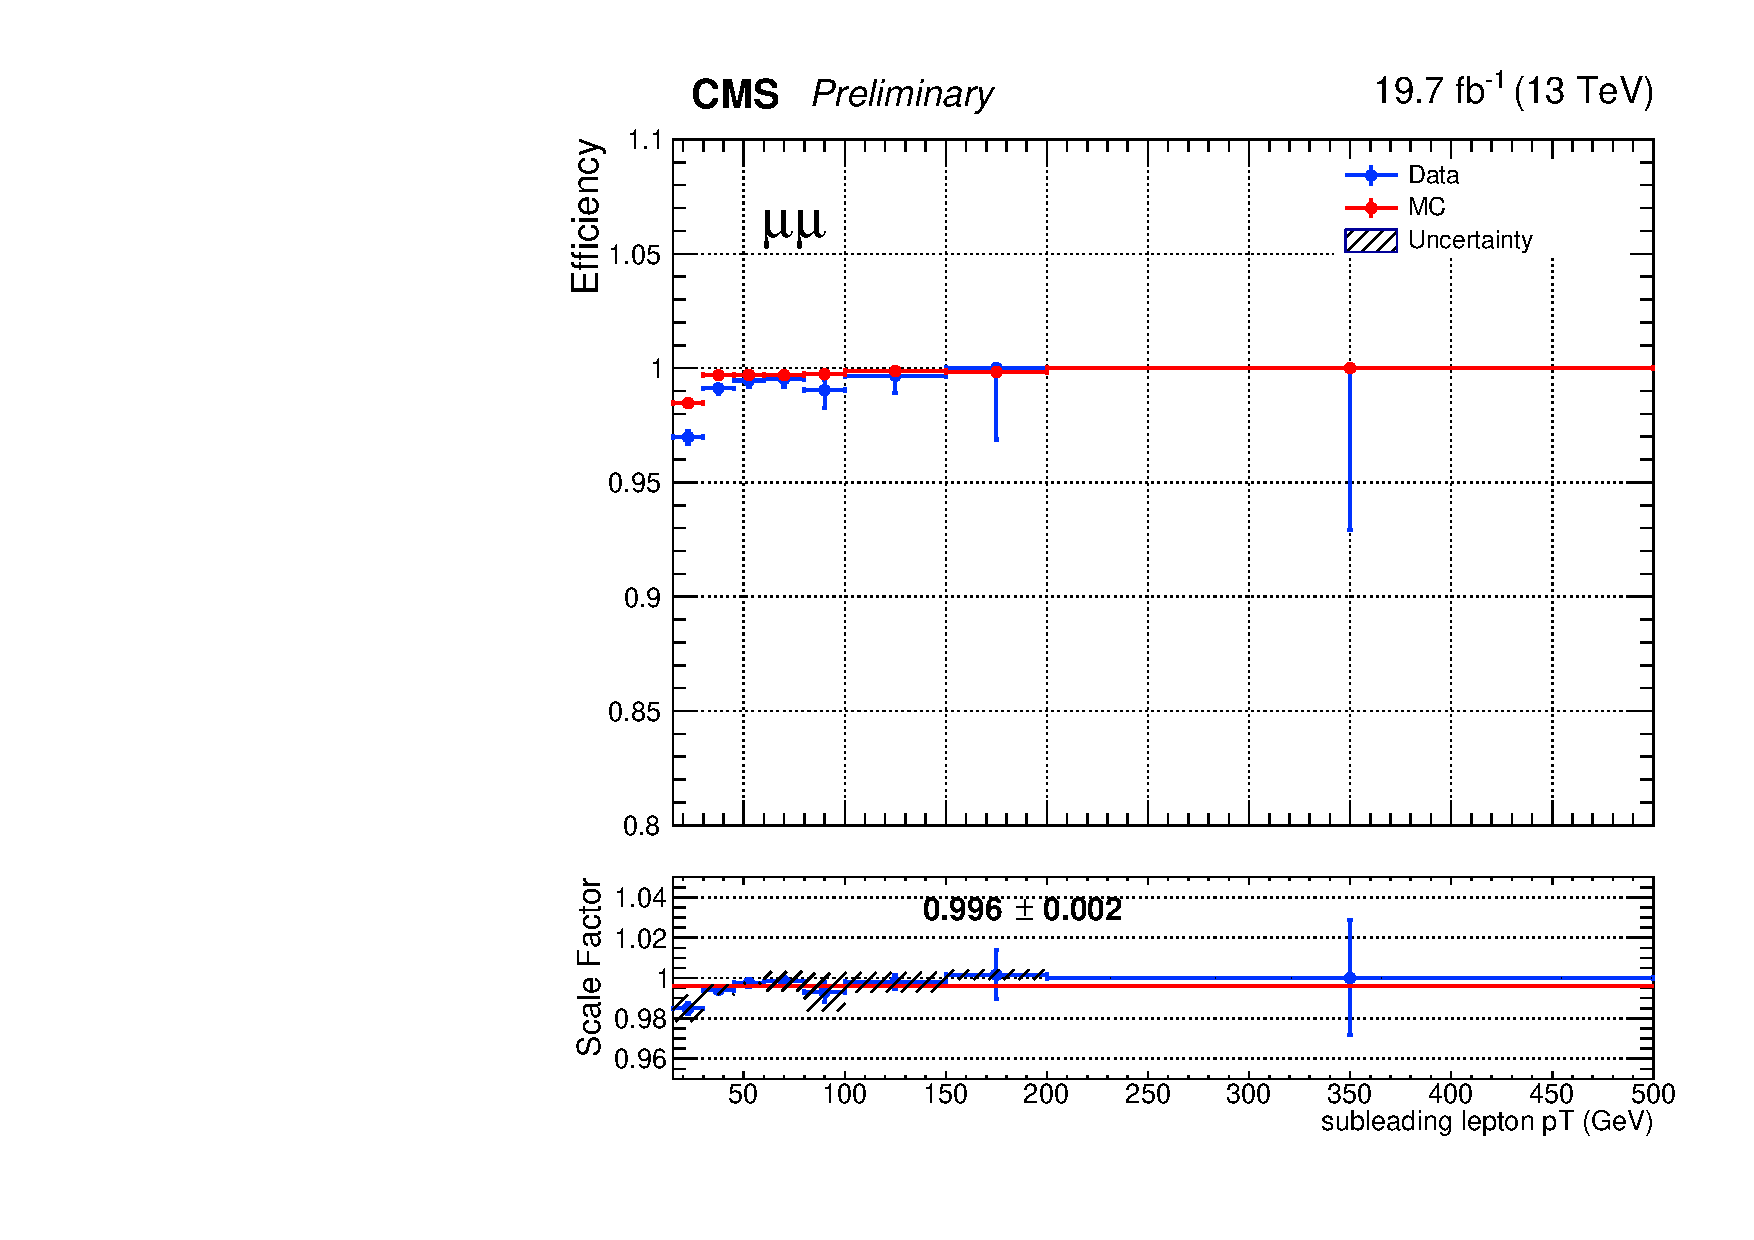
\includegraphics[width=0.32\textwidth]{fig_2016preVFP_TrigSF/g_mumu_lepBpt_FullSystUncBand.pdf}\\
    \end{tabular}
    \caption{Efficiencies and scale factors for the 2016preVFP data set in the \mumu channel as a function of leading and sub-leading lepton \pT.
            The error bars indicate the statistical uncertainty, and the shaded band corresponds to the systematic uncertainty.
            }
    \label{TrigSF_2016preVFP_3}
  \end{center}
\end{figure}

\begin{figure}[h]
  \begin{center}
    \begin{tabular}{cc}
      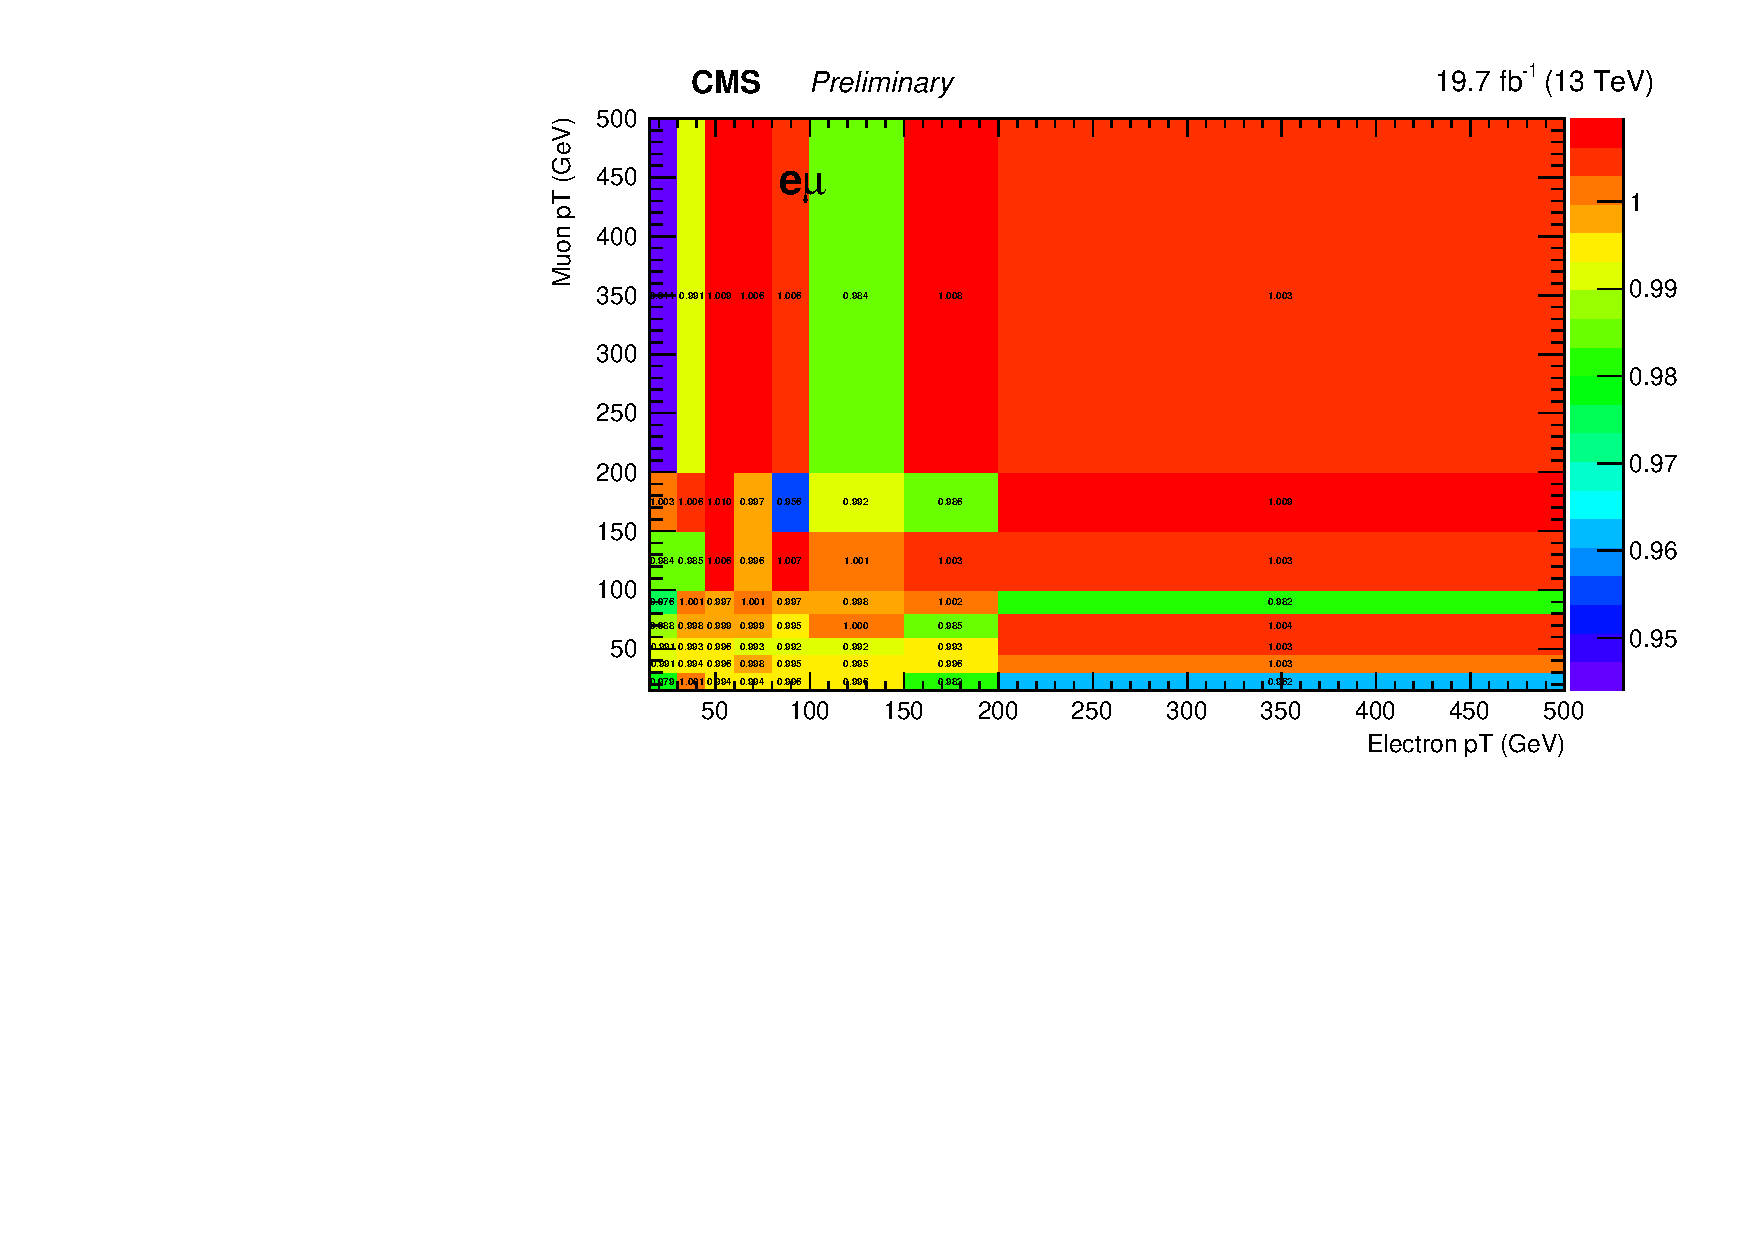
\includegraphics[width=0.50\textwidth]{fig_2016preVFP_TrigSF/h2D_lepABpt_emu.pdf}
      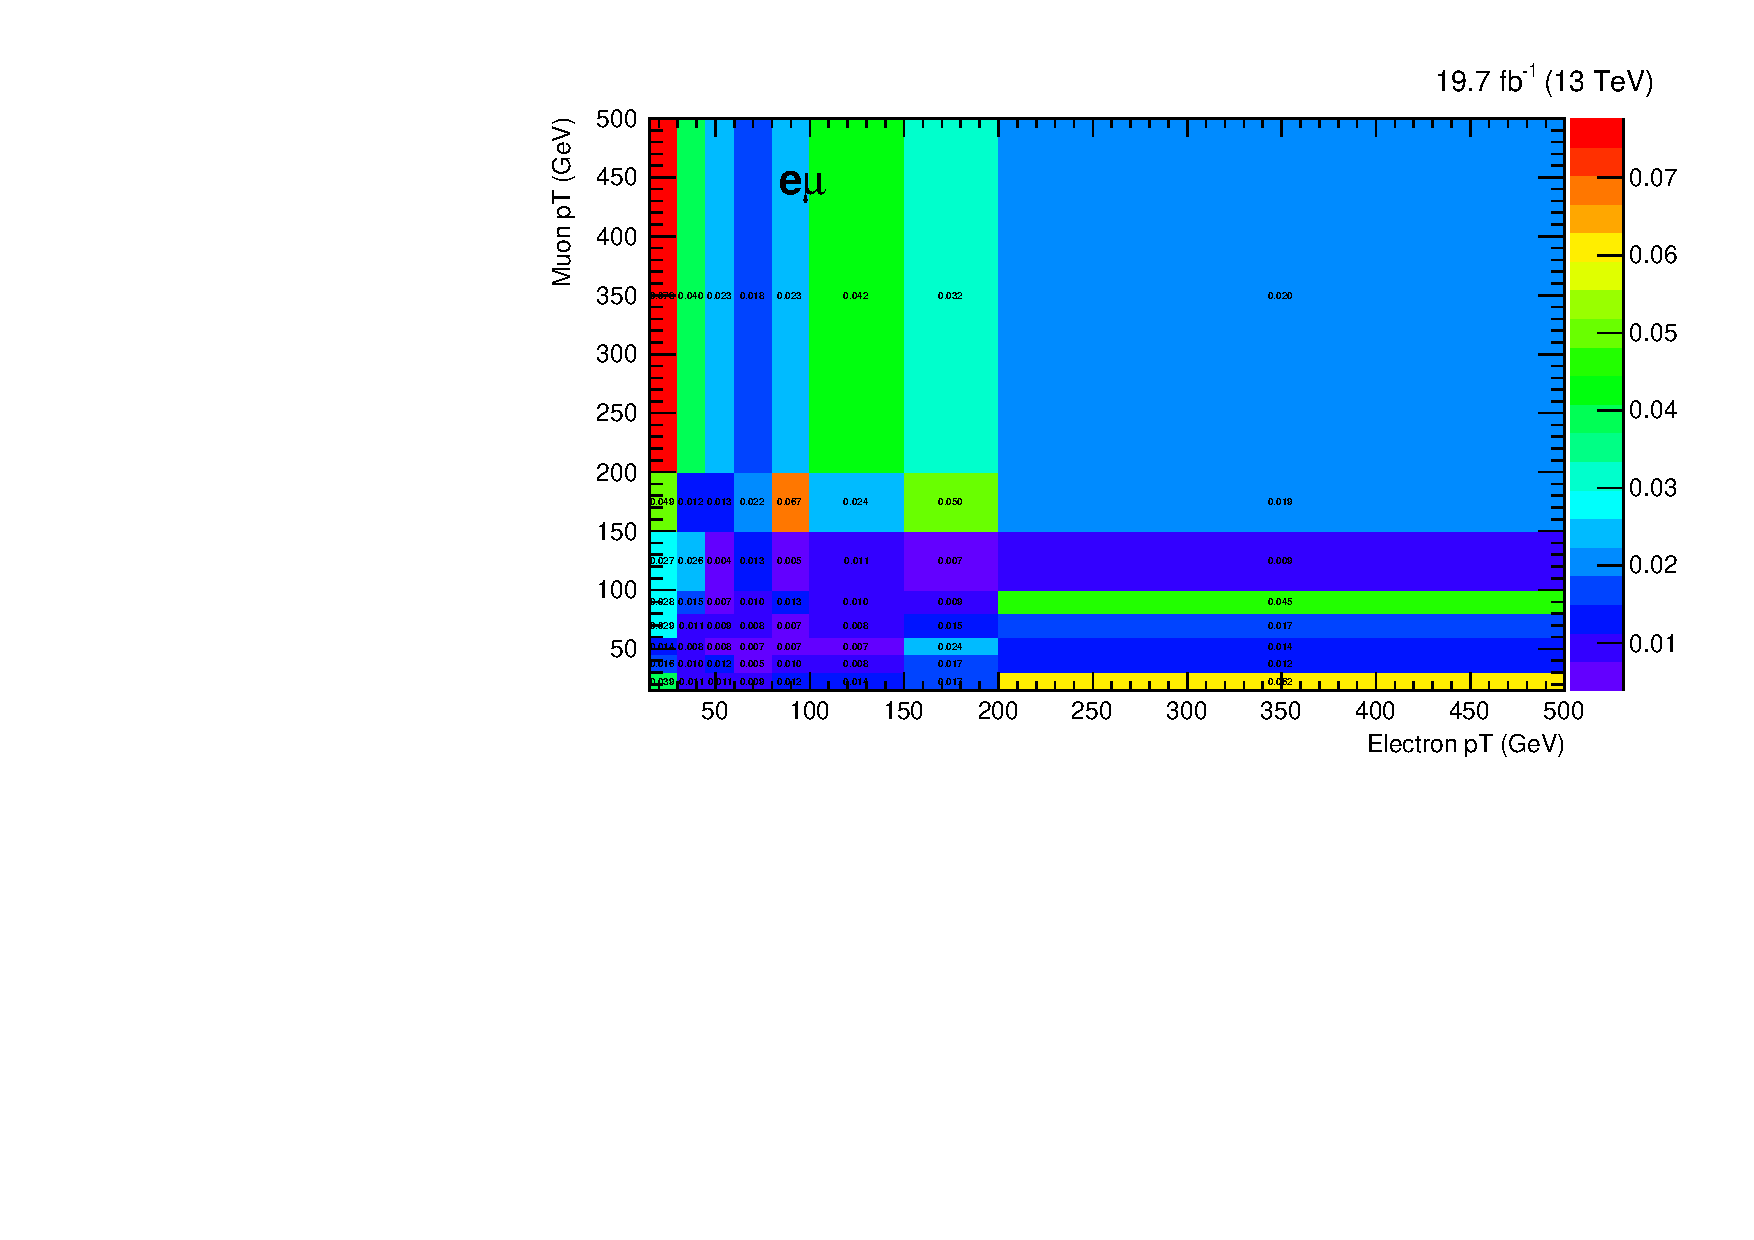
\includegraphics[width=0.50\textwidth]{fig_2016preVFP_TrigSF/h2D_lepABpt_emu_BinErrors.pdf}\\       
      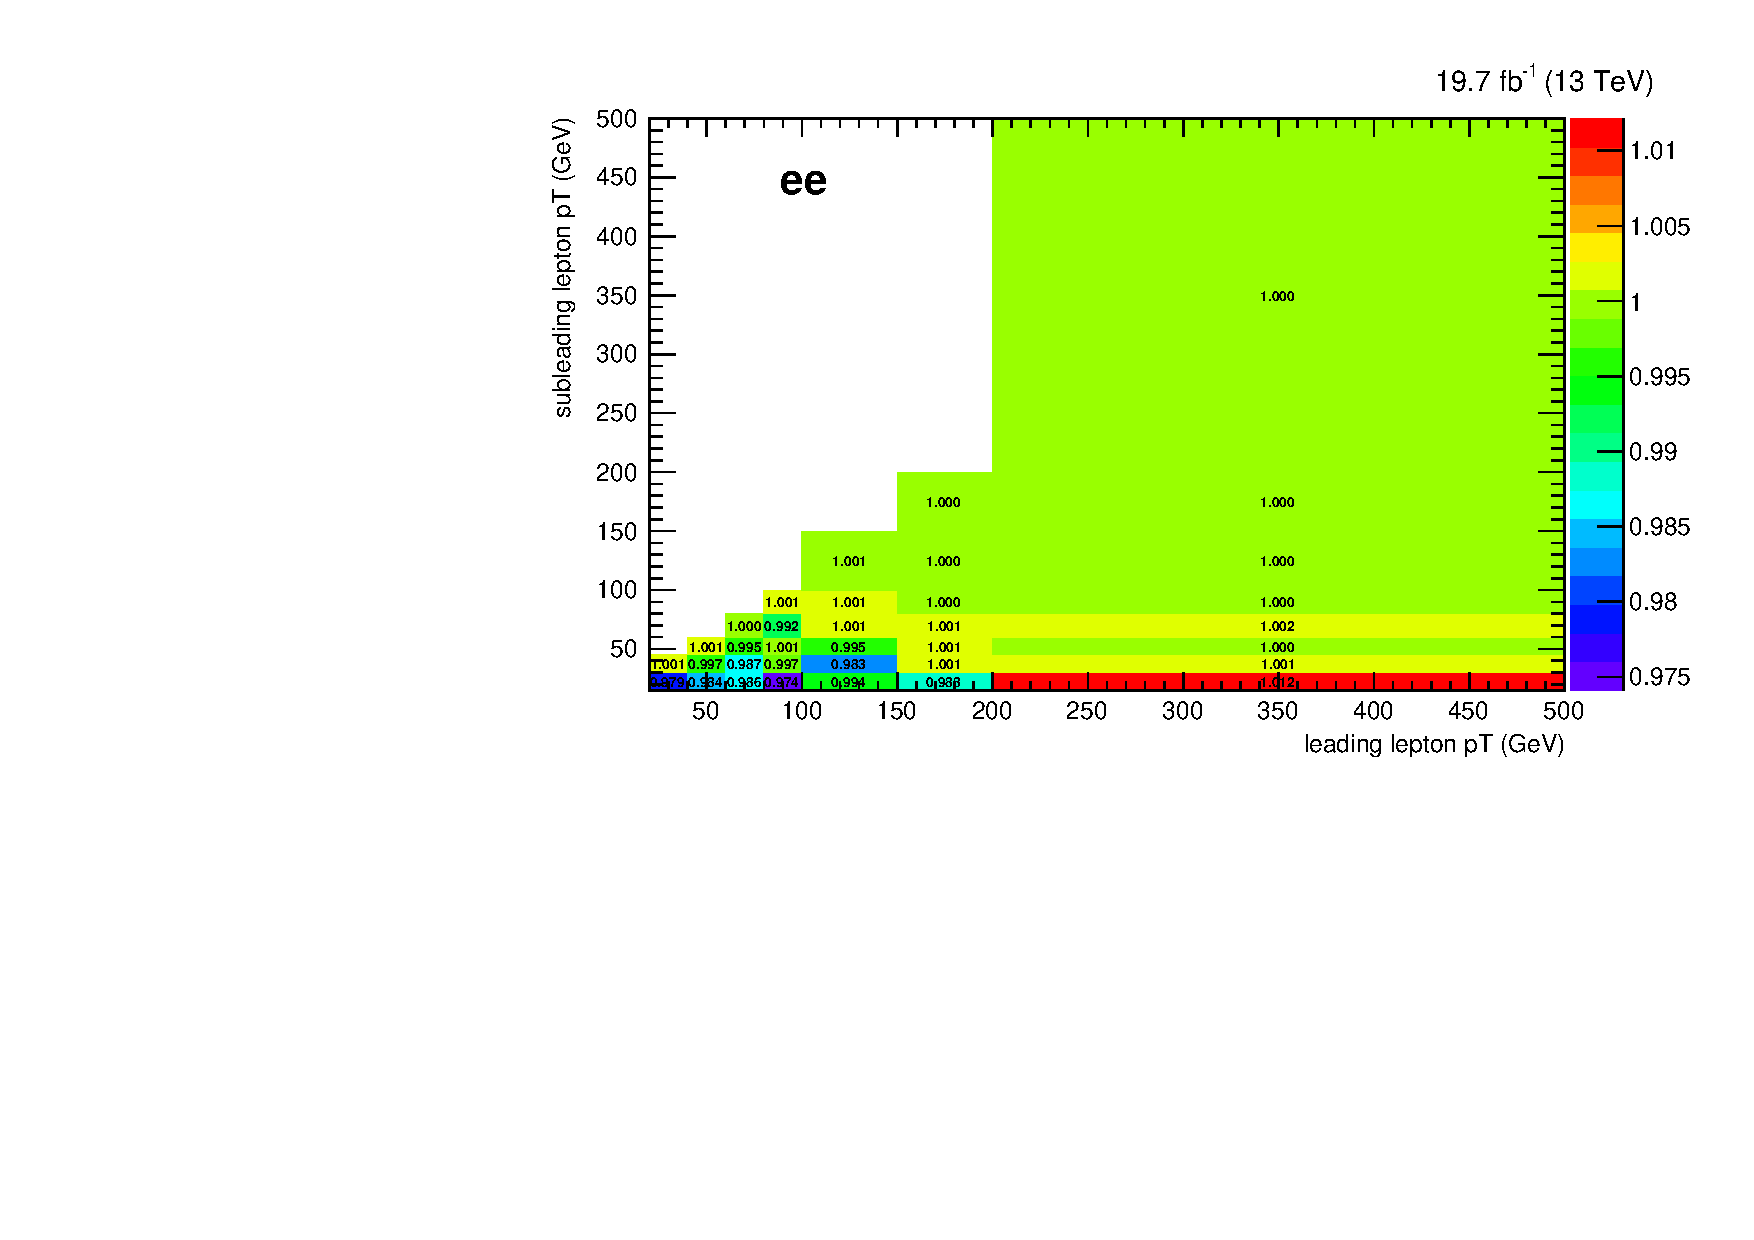
\includegraphics[width=0.50\textwidth]{fig_2016preVFP_TrigSF/h2D_lepABpt_ee.pdf}
      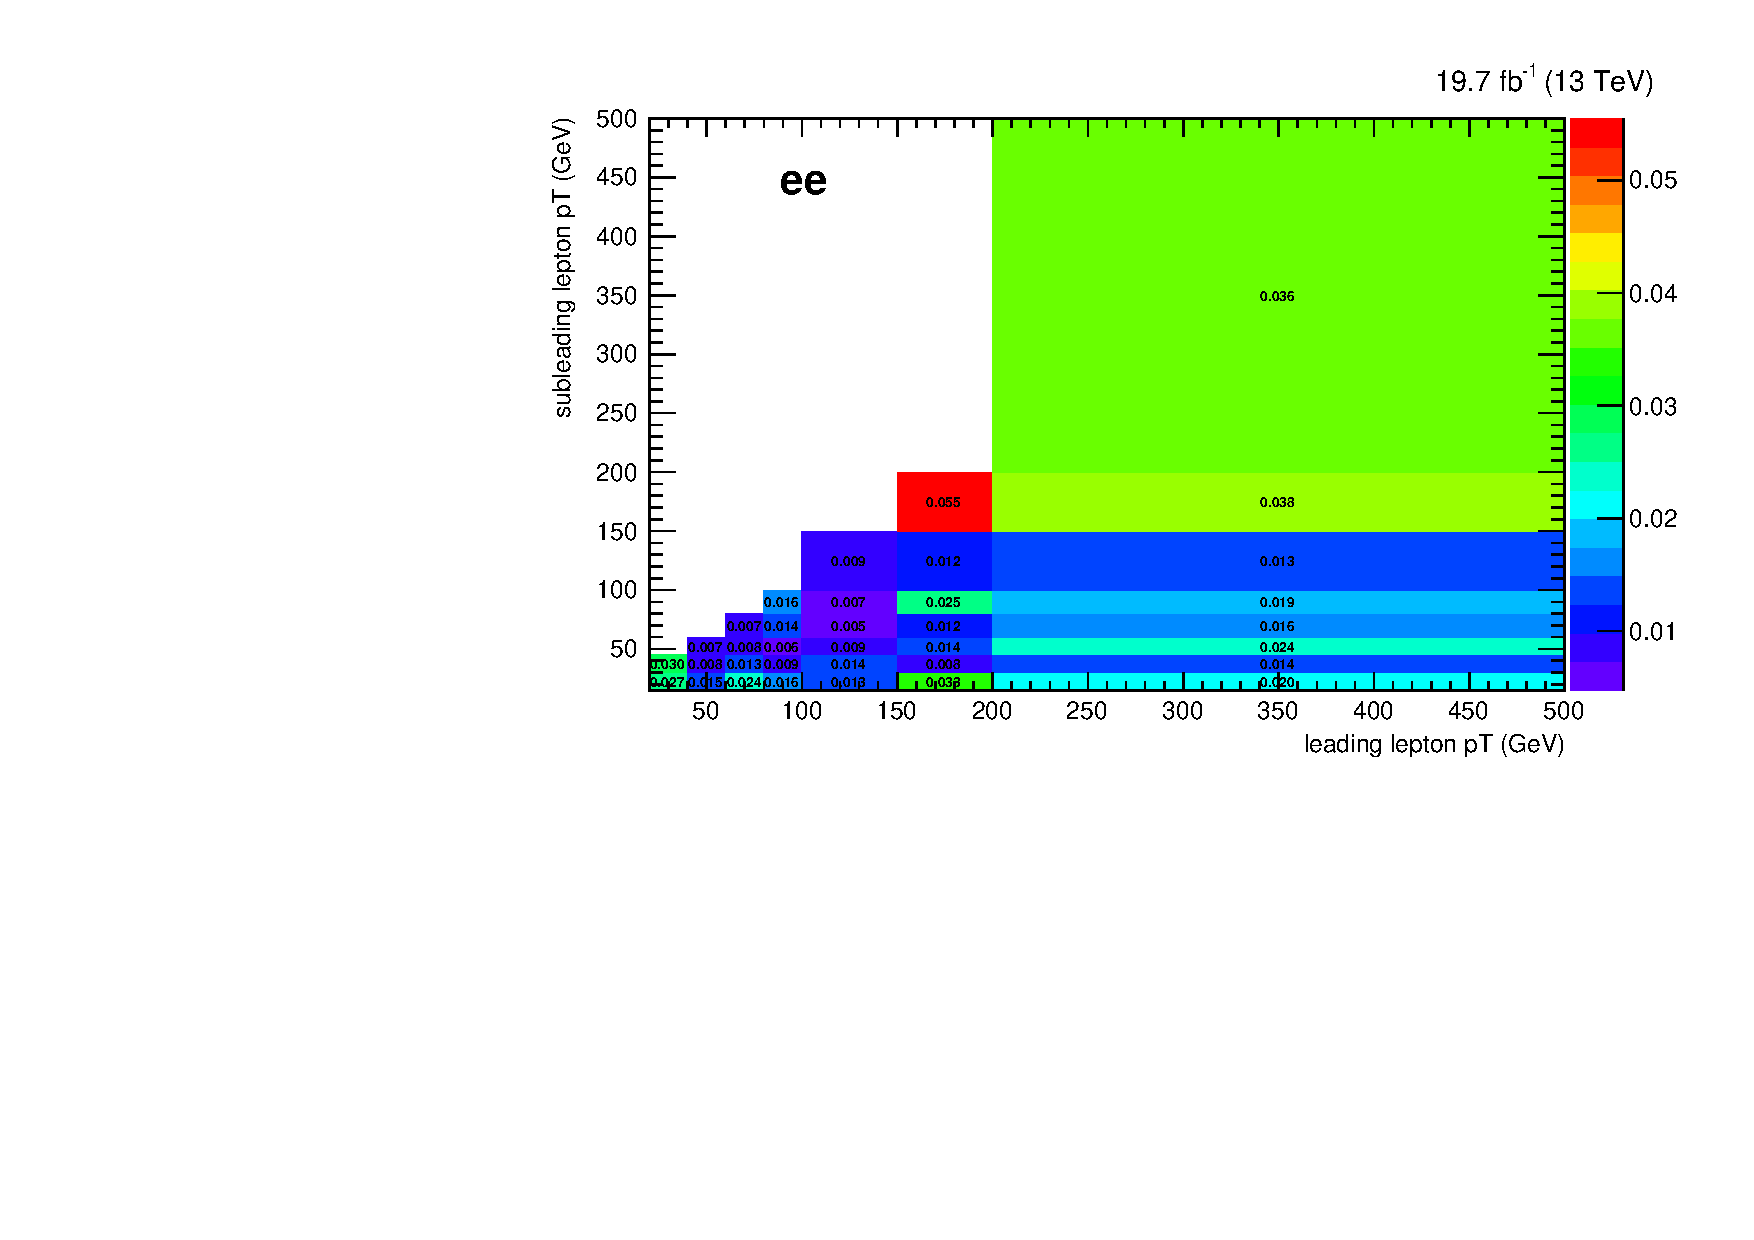
\includegraphics[width=0.50\textwidth]{fig_2016preVFP_TrigSF/h2D_lepABpt_ee_BinErrors.pdf}\\
      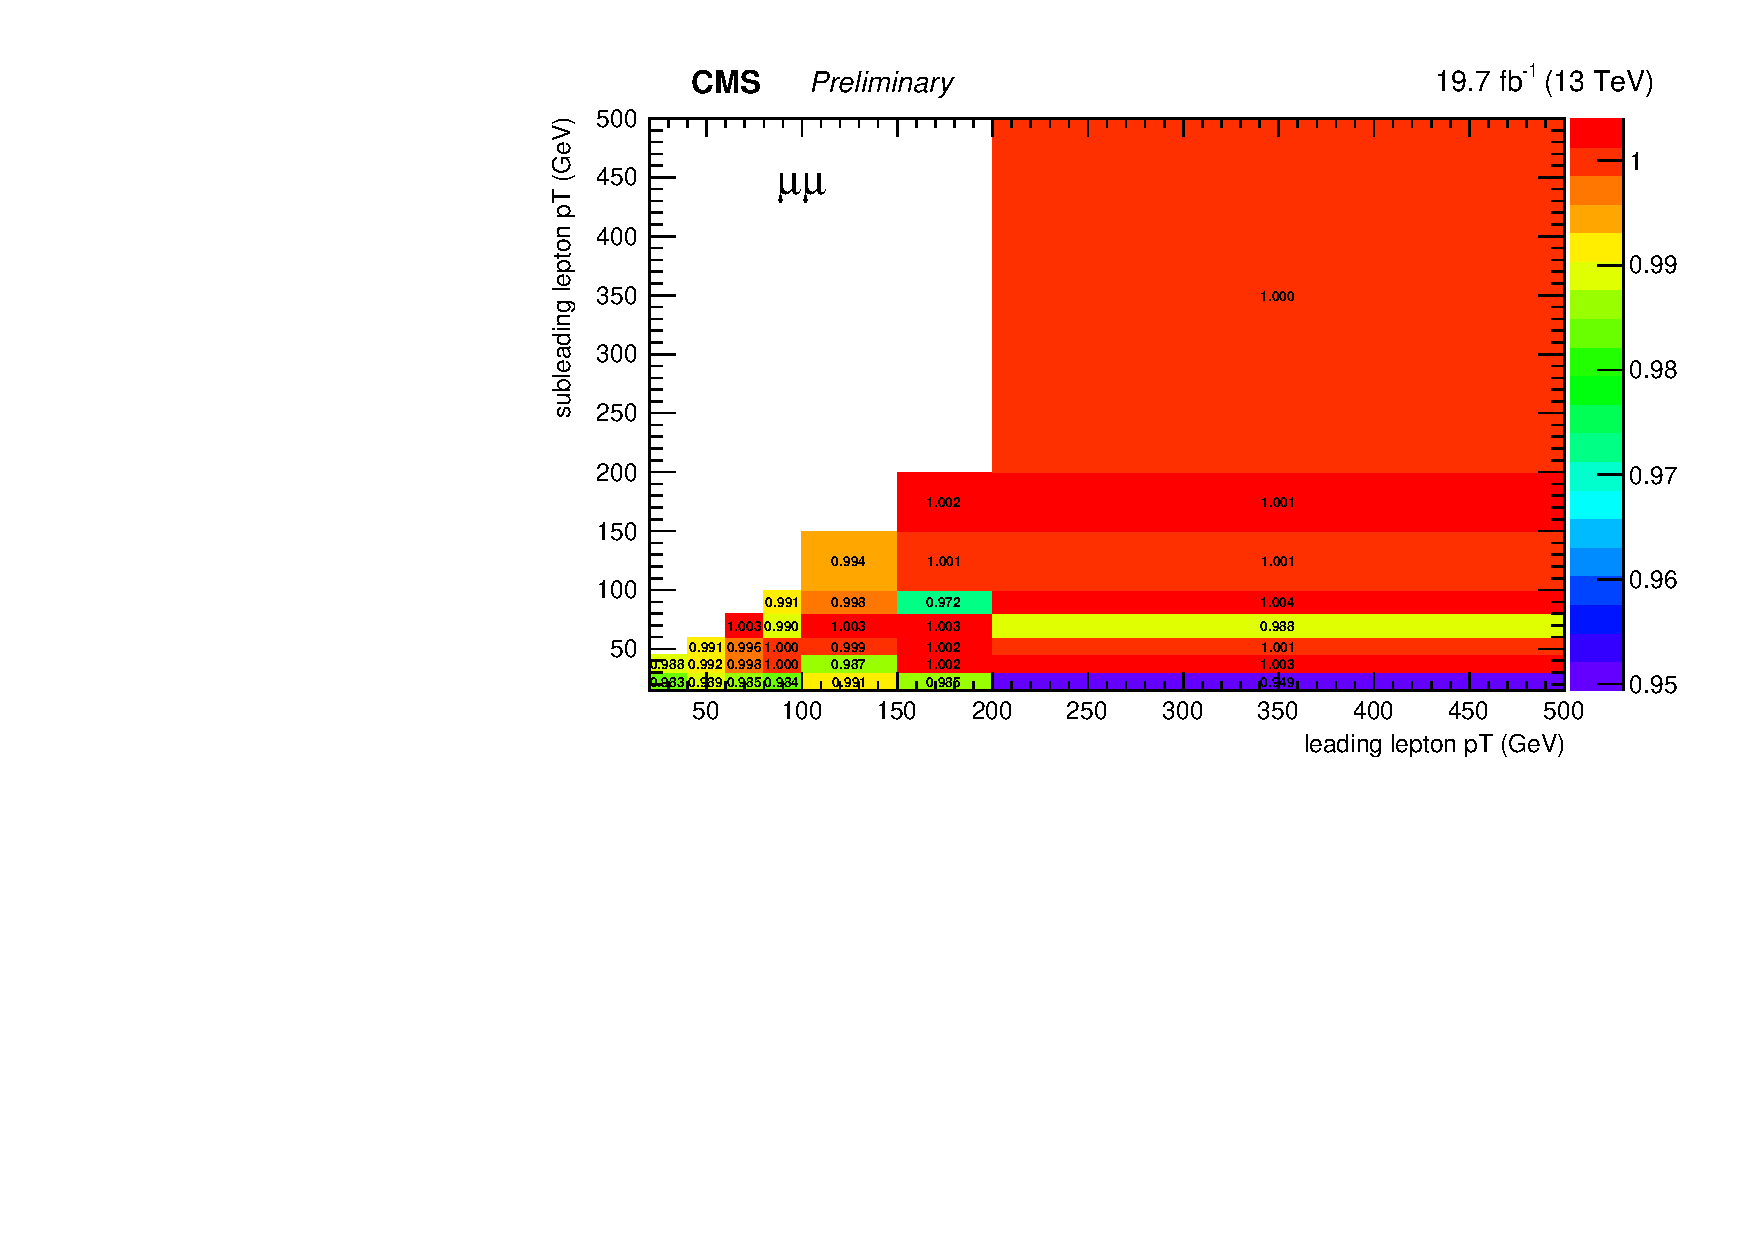
\includegraphics[width=0.50\textwidth]{fig_2016preVFP_TrigSF/h2D_lepABpt_mumu.pdf}
      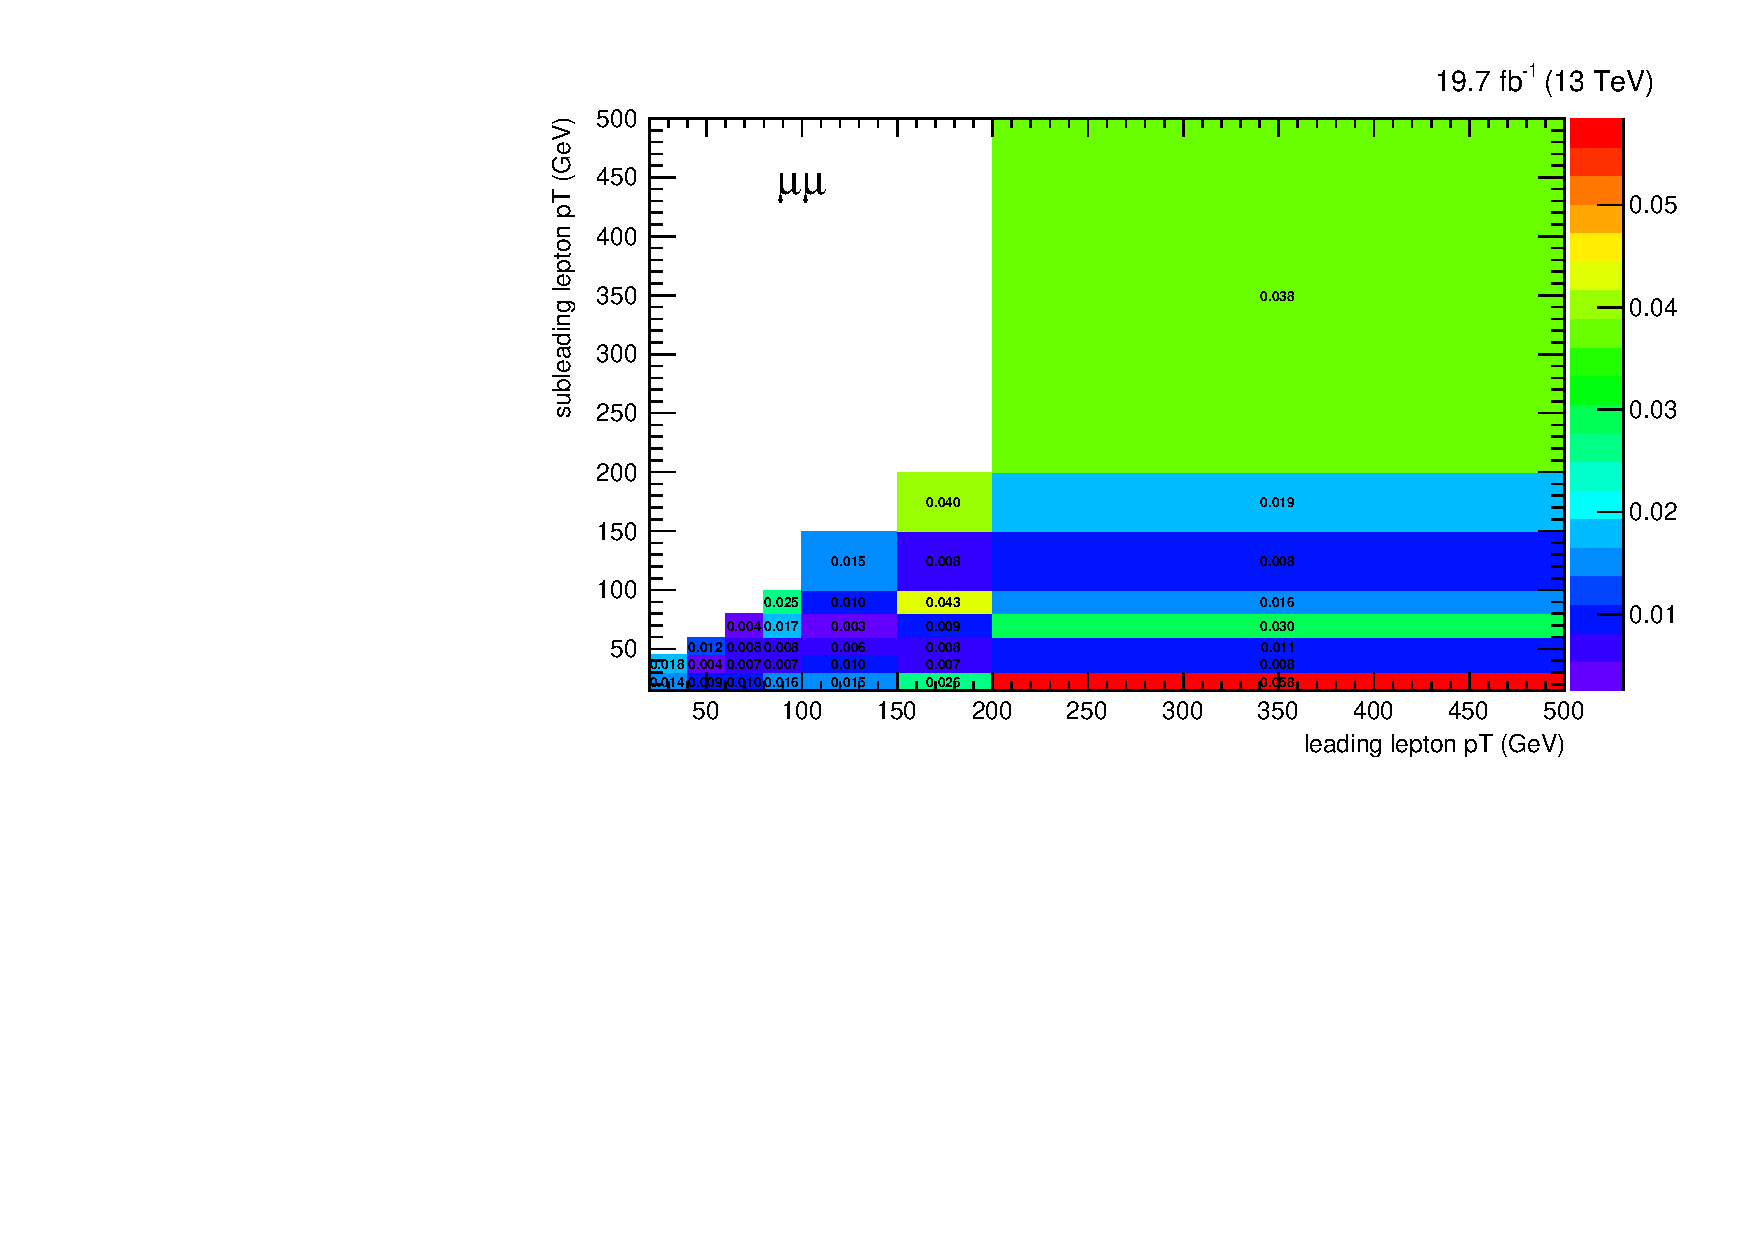
\includegraphics[width=0.50\textwidth]{fig_2016preVFP_TrigSF/h2D_lepABpt_mumu_BinErrors.pdf}\\
    \end{tabular}
    \caption{2D scale factors (Left) and total uncertainties (Right) for the 2016preVFP data set in the \emu (top), \ee (middle) and \mumu (bottom) channels as a function of leading lepton \pT and sub-leading lepton \pT.}
    \label{TrigSF_2016preVFP_4}
  \end{center}
\end{figure}

\clearpage
\subsection{Trigger Efficiencies and Scale Factors: 2016postVFP}
\label{TrigSFResults2016postVFP}

\begin{figure}[h]
  \begin{center}
    \begin{tabular}{ccc}
      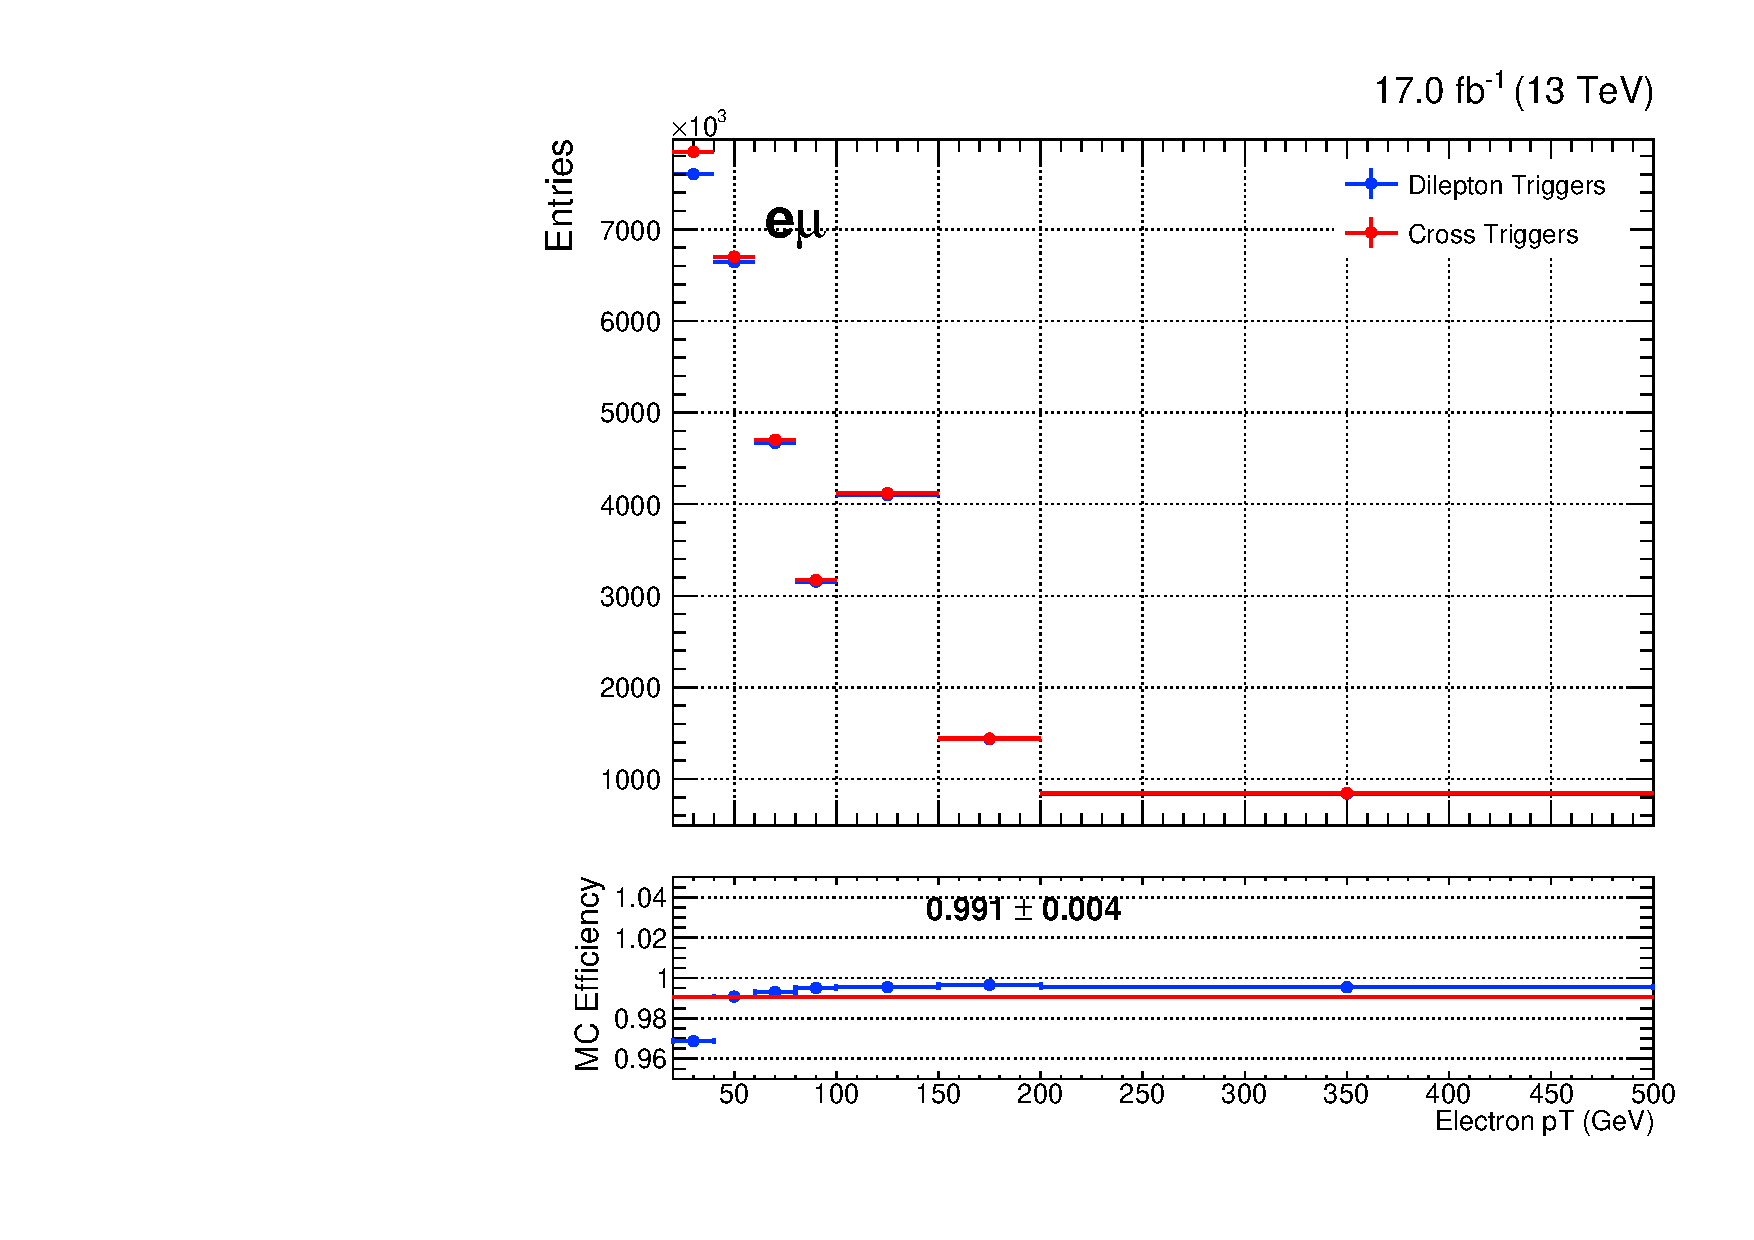
\includegraphics[width=0.32\textwidth]{fig_2016postVFP_TrigSF/g_lepApt_emu_MC.pdf}
      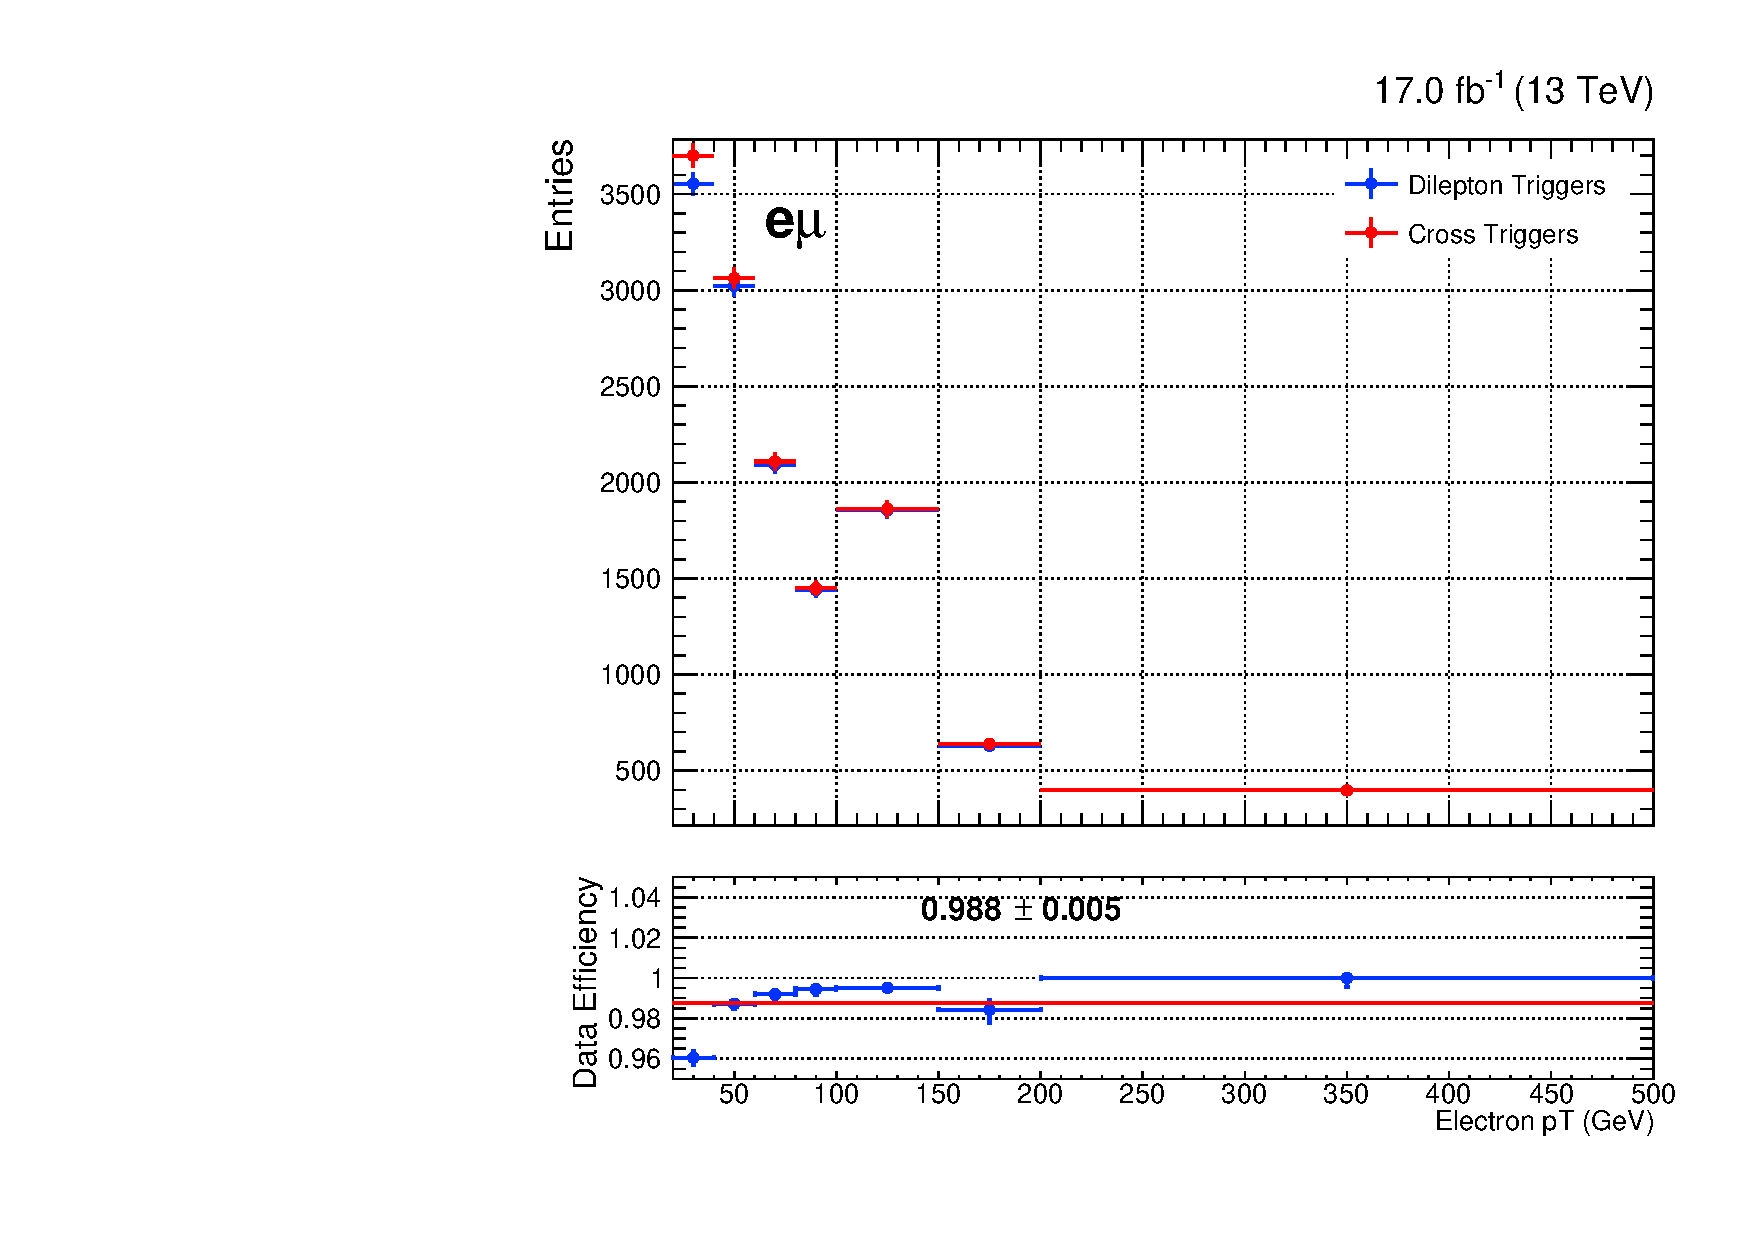
\includegraphics[width=0.32\textwidth]{fig_2016postVFP_TrigSF/g_lepApt_emu_data.pdf}
      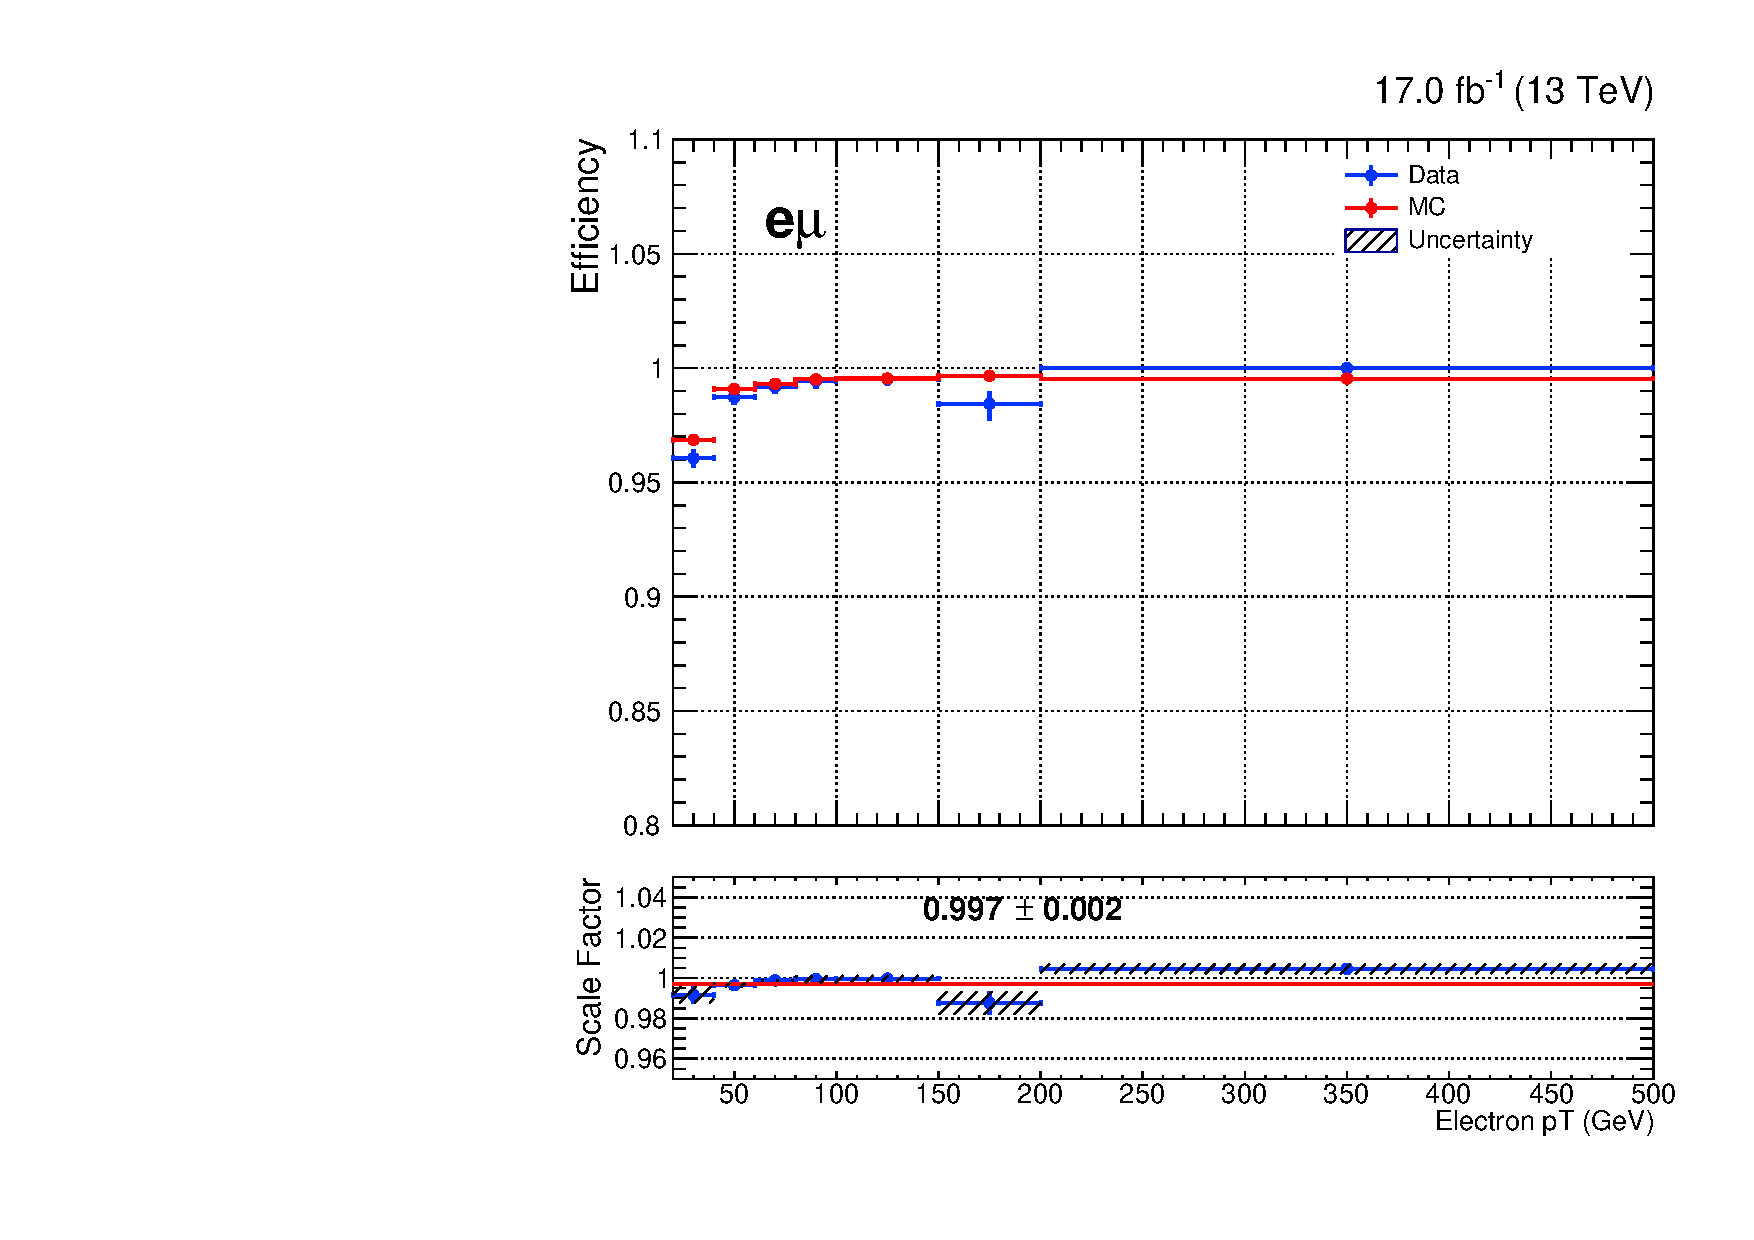
\includegraphics[width=0.32\textwidth]{fig_2016postVFP_TrigSF/g_emu_lepApt_FullSystUncBand.pdf}\\
      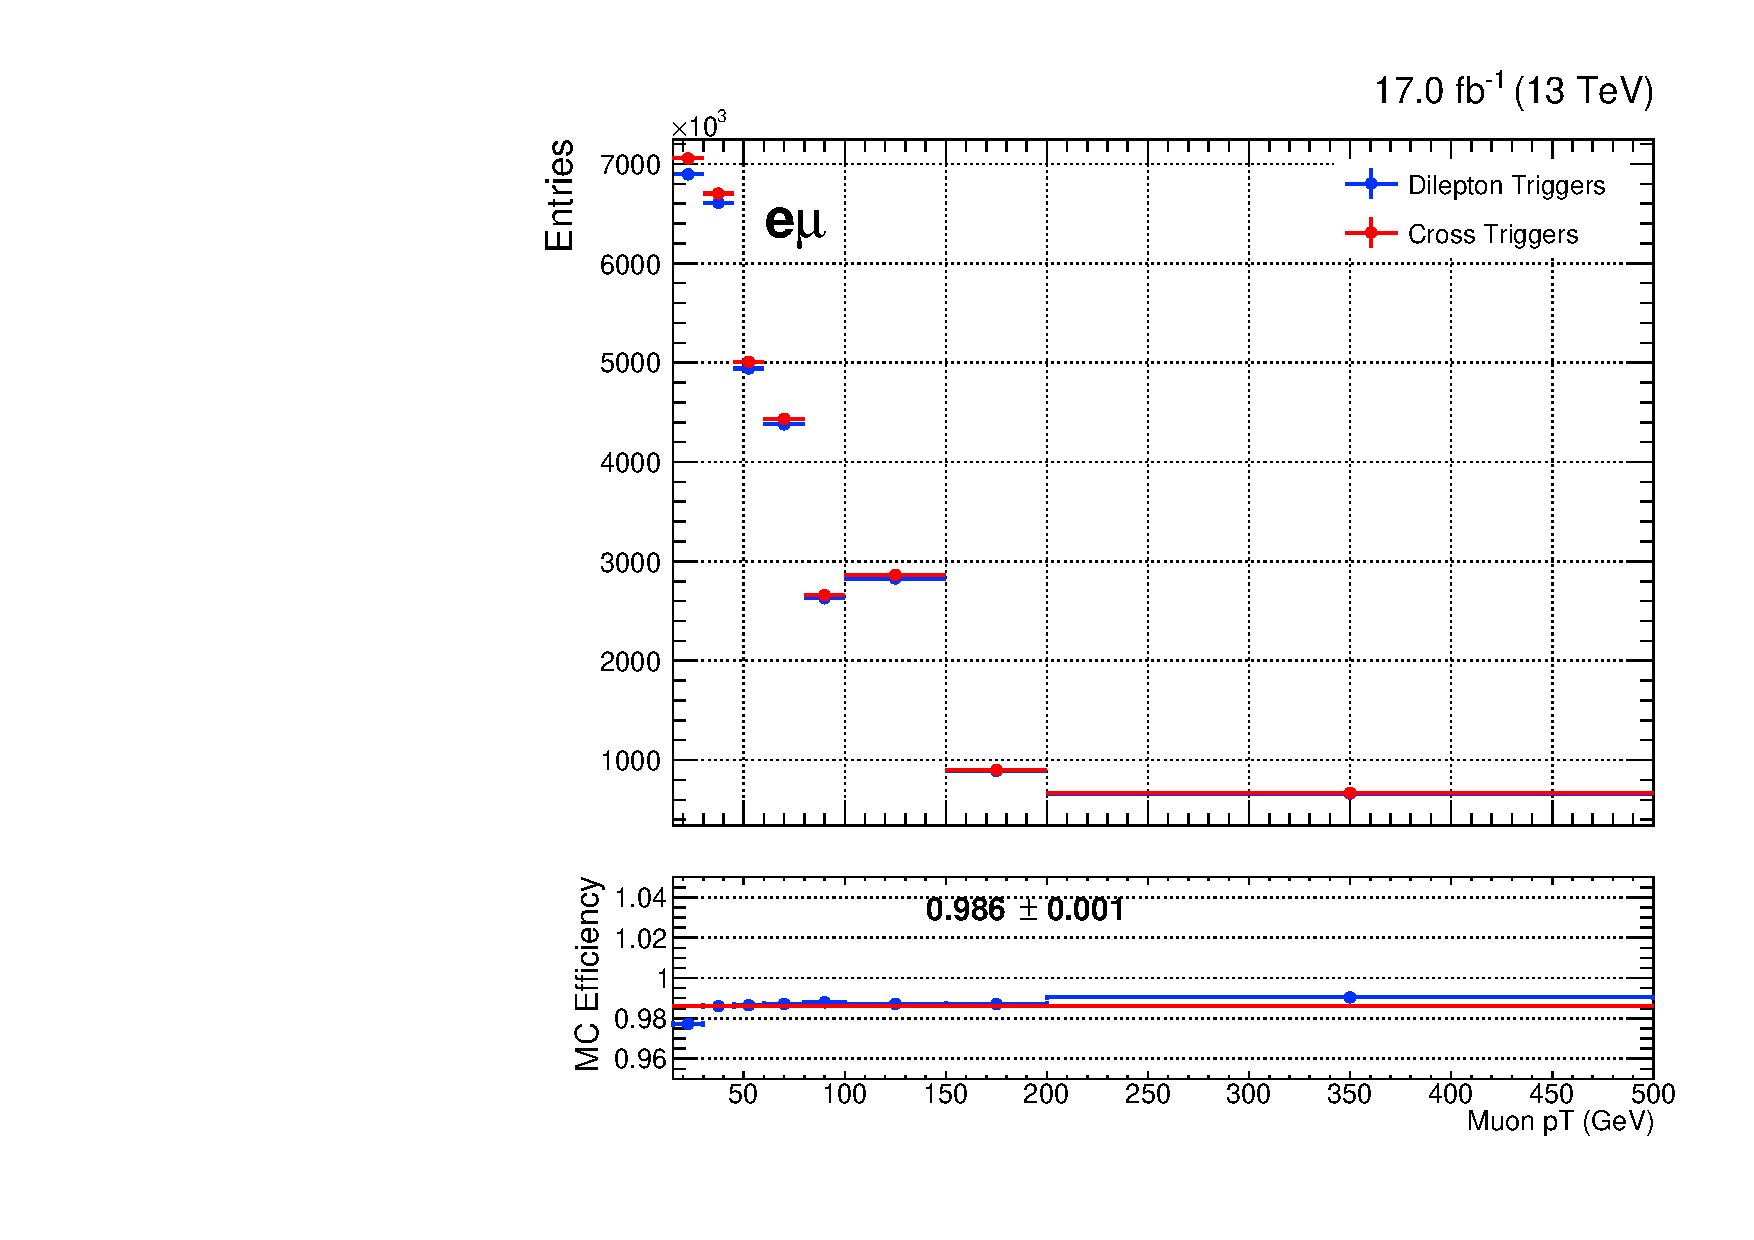
\includegraphics[width=0.32\textwidth]{fig_2016postVFP_TrigSF/g_lepBpt_emu_MC.pdf}
      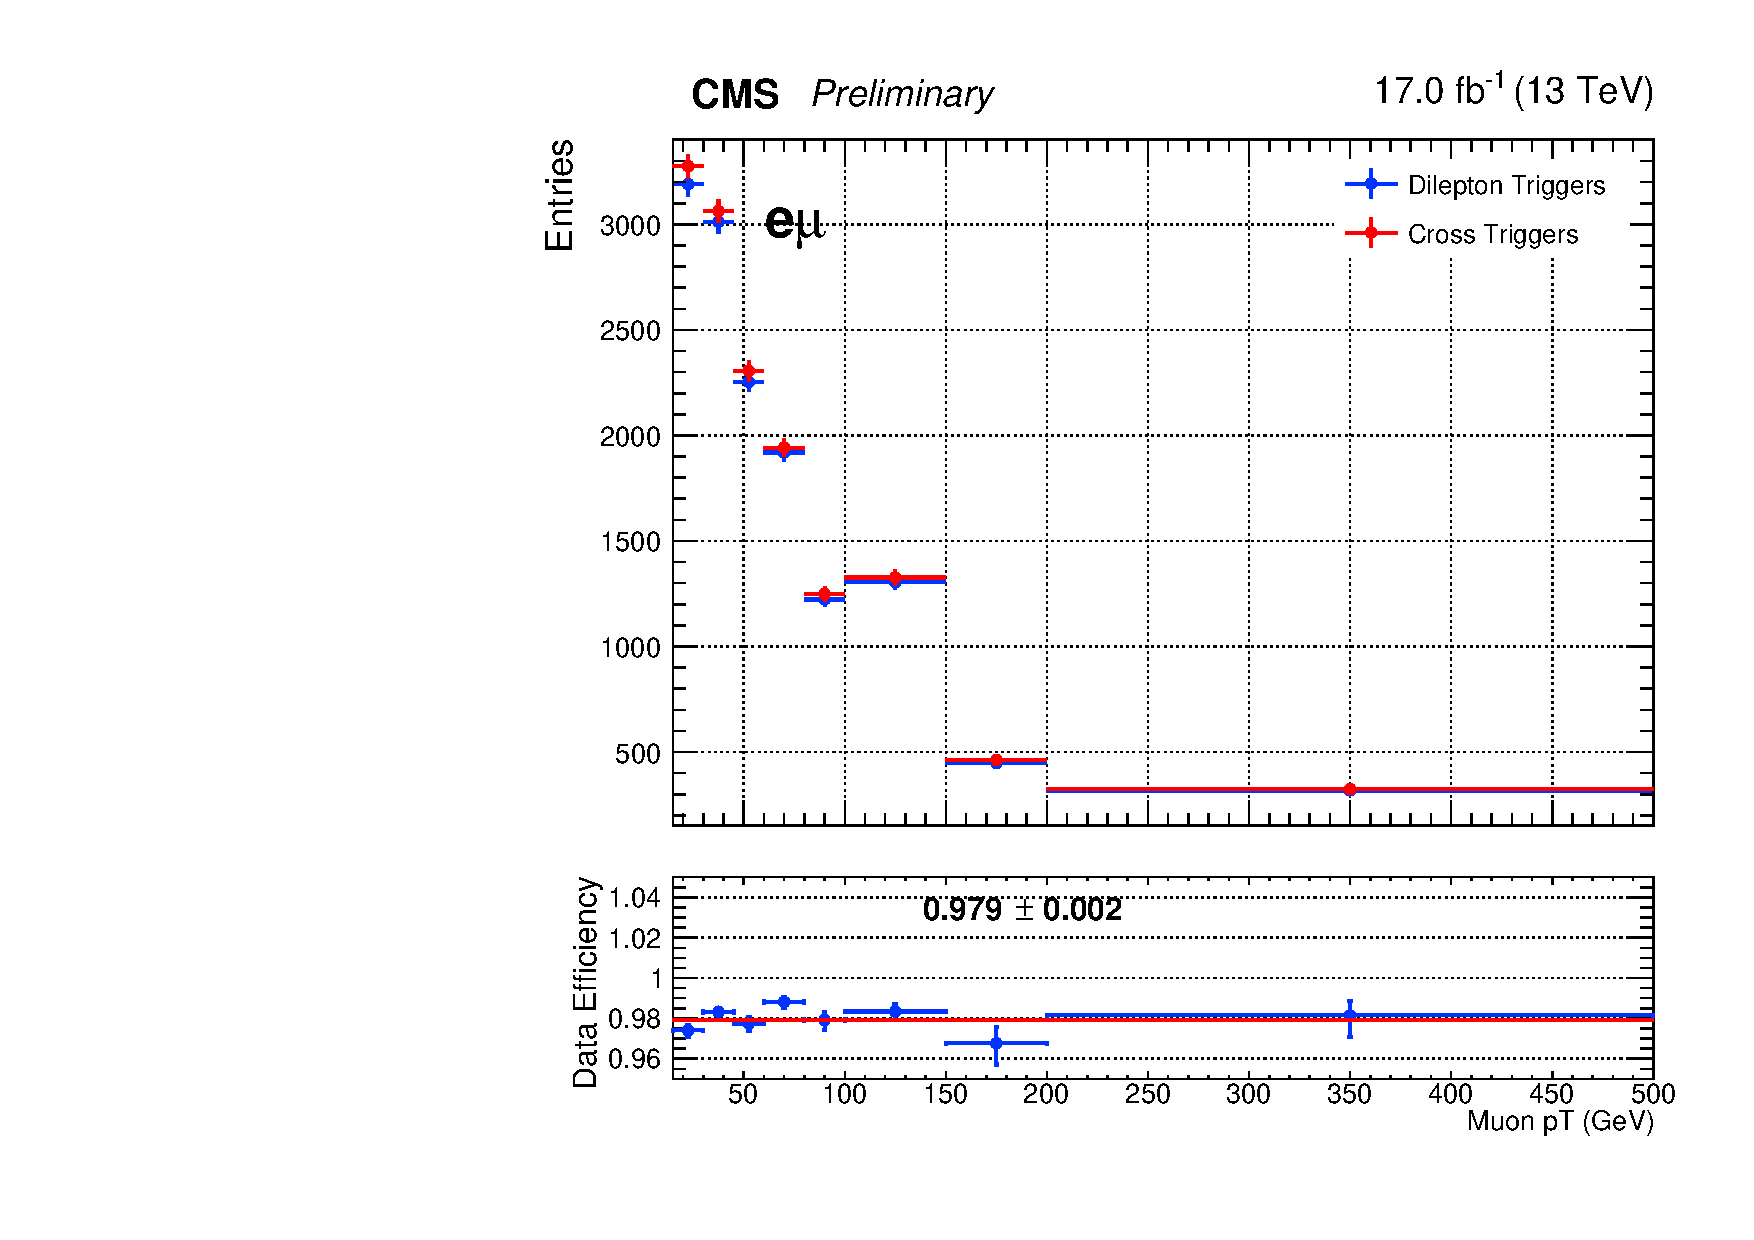
\includegraphics[width=0.32\textwidth]{fig_2016postVFP_TrigSF/g_lepBpt_emu_data.pdf}
      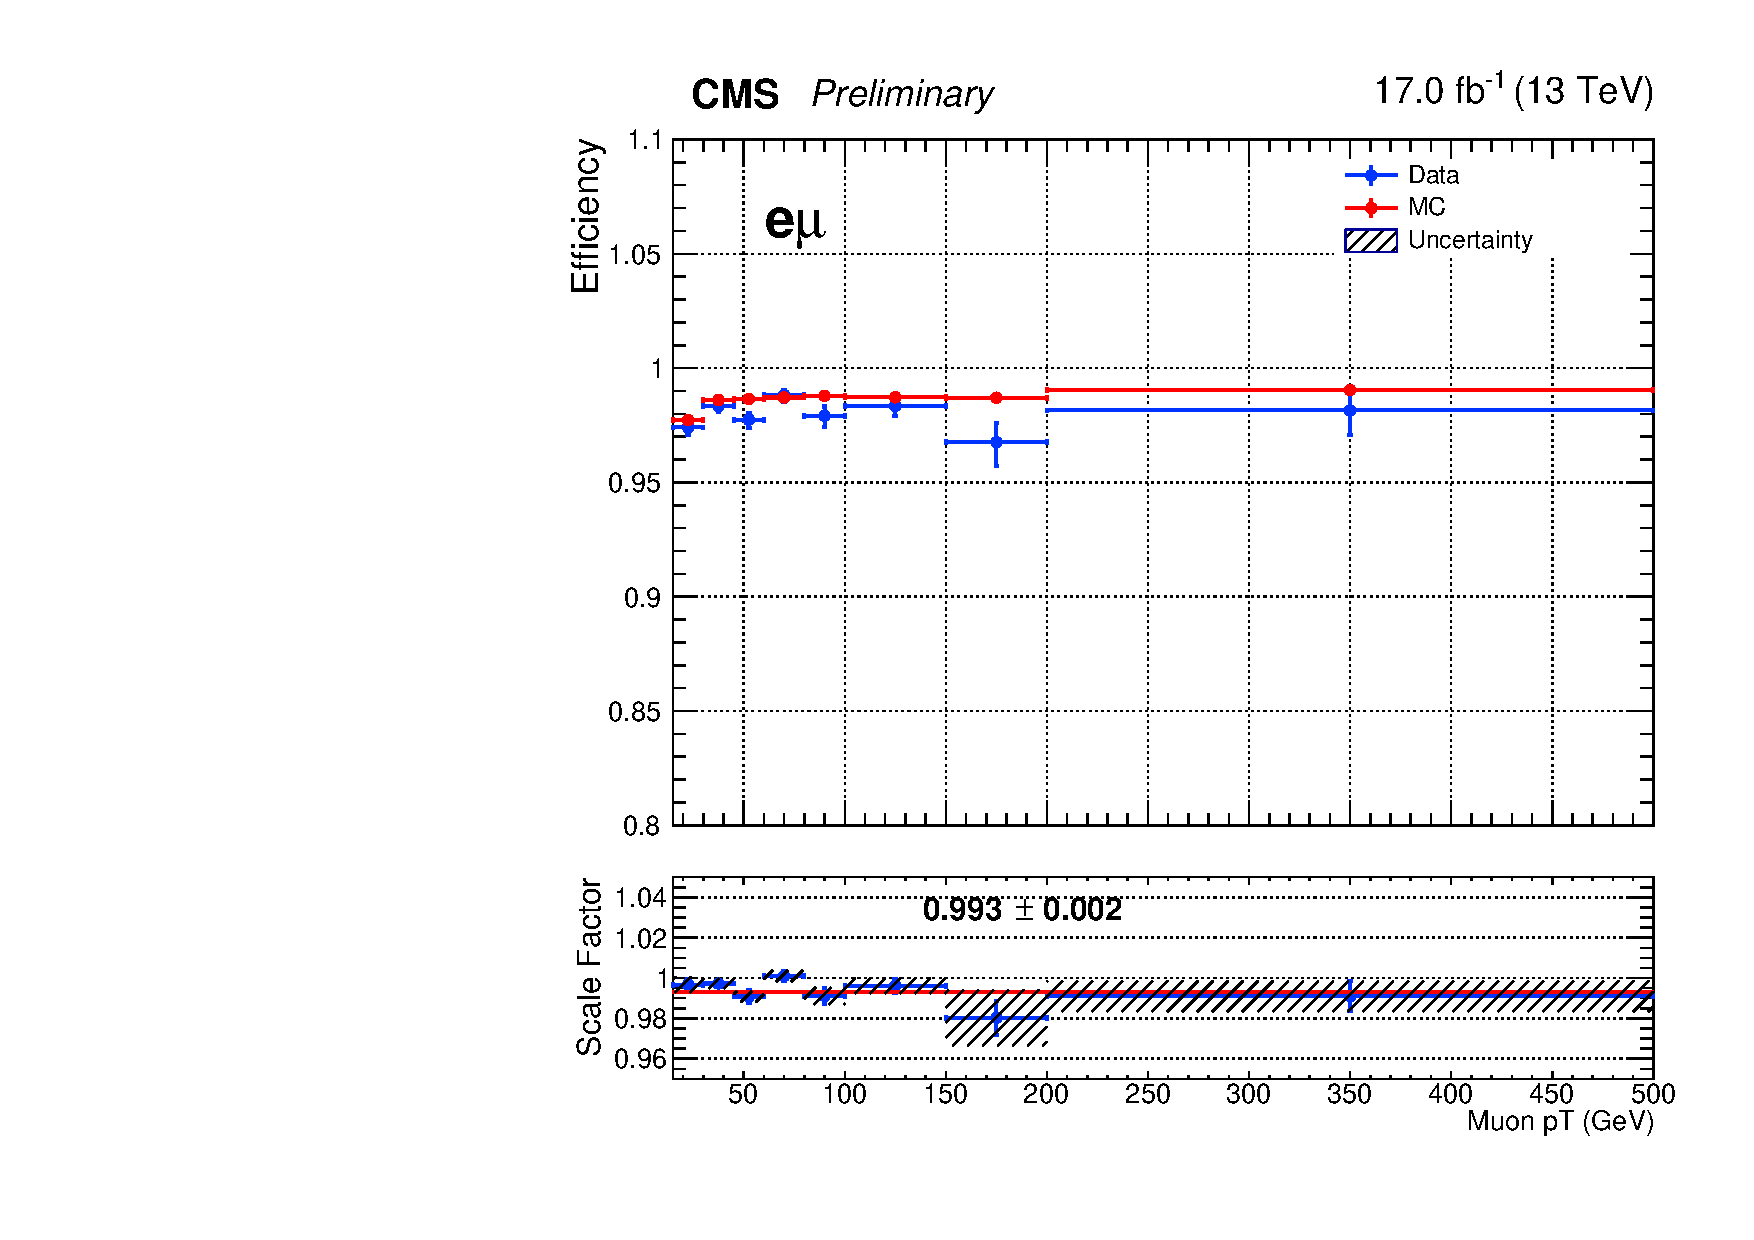
\includegraphics[width=0.32\textwidth]{fig_2016postVFP_TrigSF/g_emu_lepBpt_FullSystUncBand.pdf}\\
    \end{tabular}
    \caption{Efficiencies and scale factors for the 2016postVFP data set in the \emu channel as a function of electron and muon \pT.
            The error bars indicate the statistical uncertainty, and the shaded band corresponds to the systematic uncertainty.
            }
    \label{TrigSF_2016postVFP_1}
  \end{center}
\end{figure}

\begin{figure}[h]
  \begin{center}
    \begin{tabular}{ccc}
      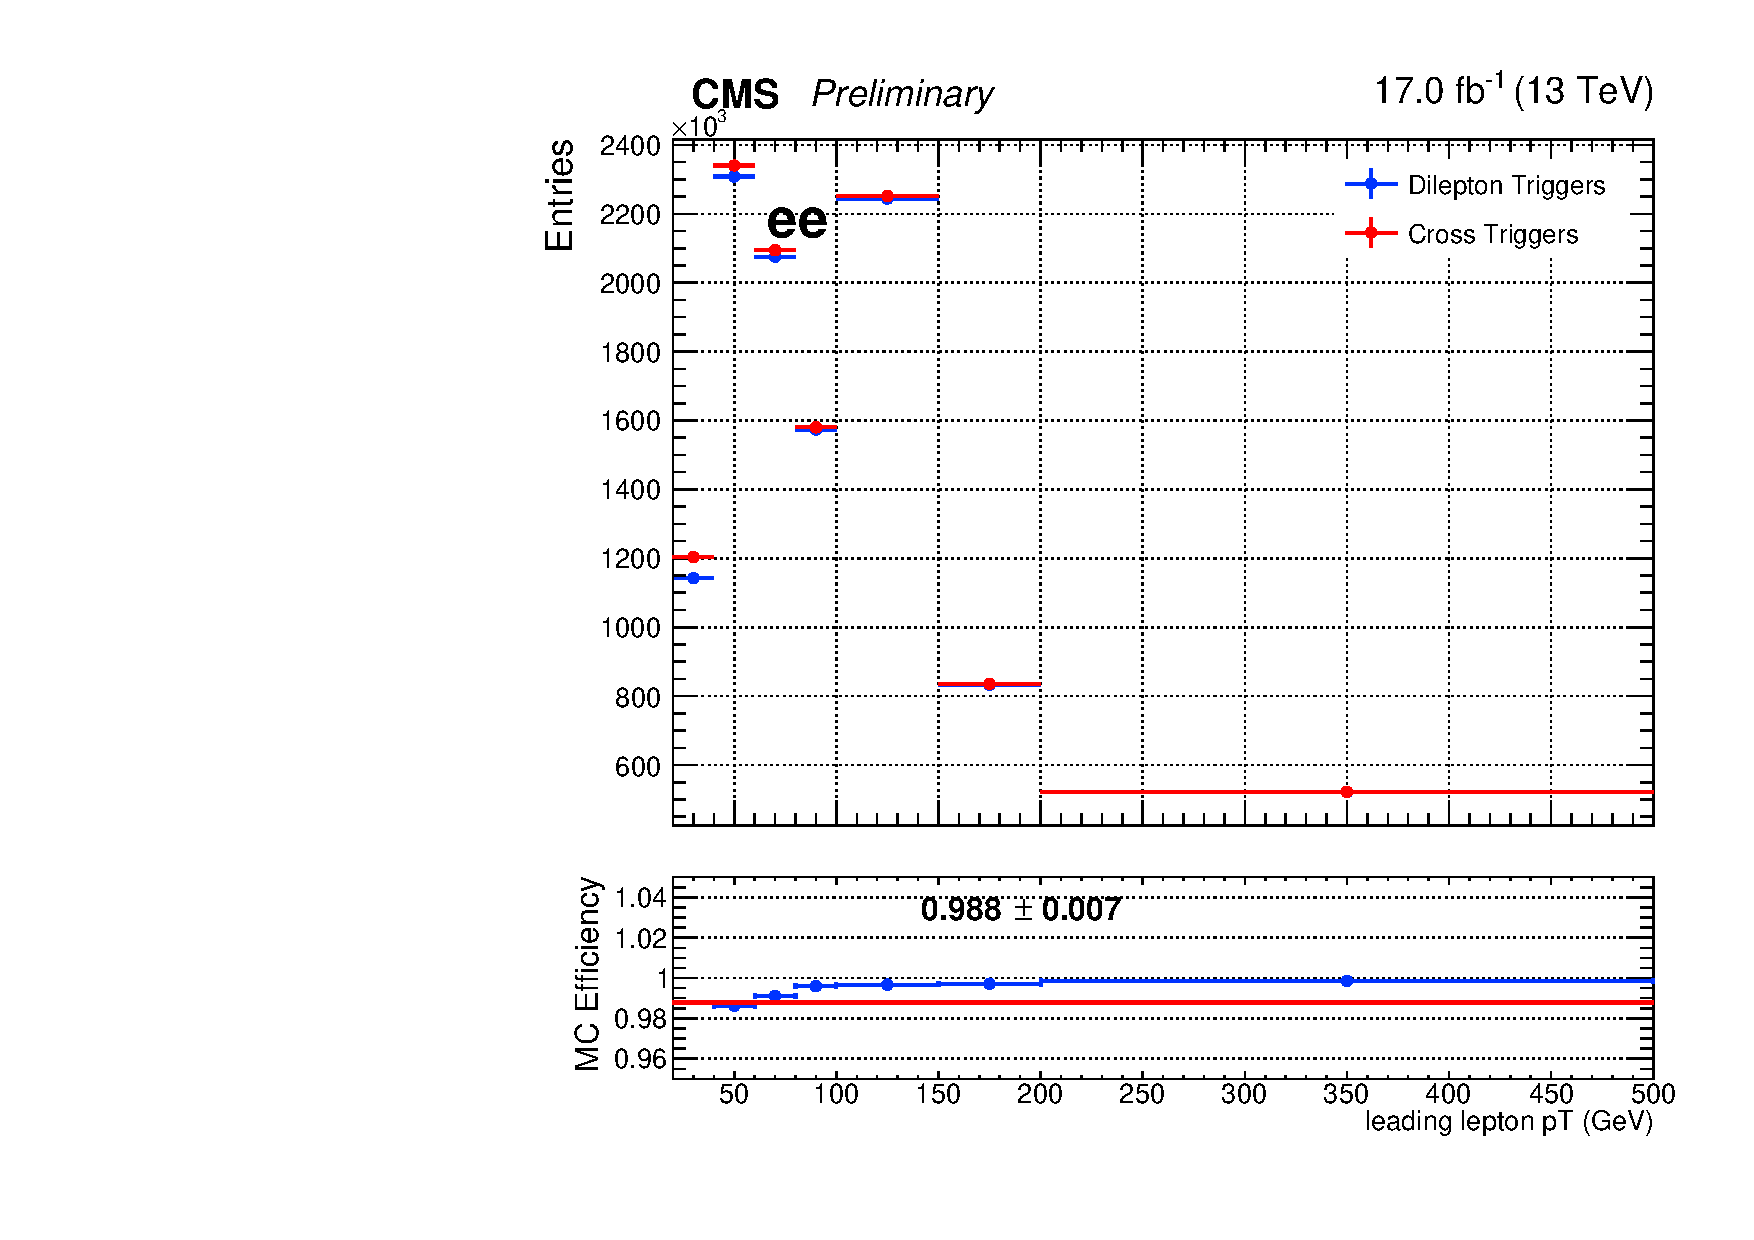
\includegraphics[width=0.32\textwidth]{fig_2016postVFP_TrigSF/g_lepApt_ee_MC.pdf}
      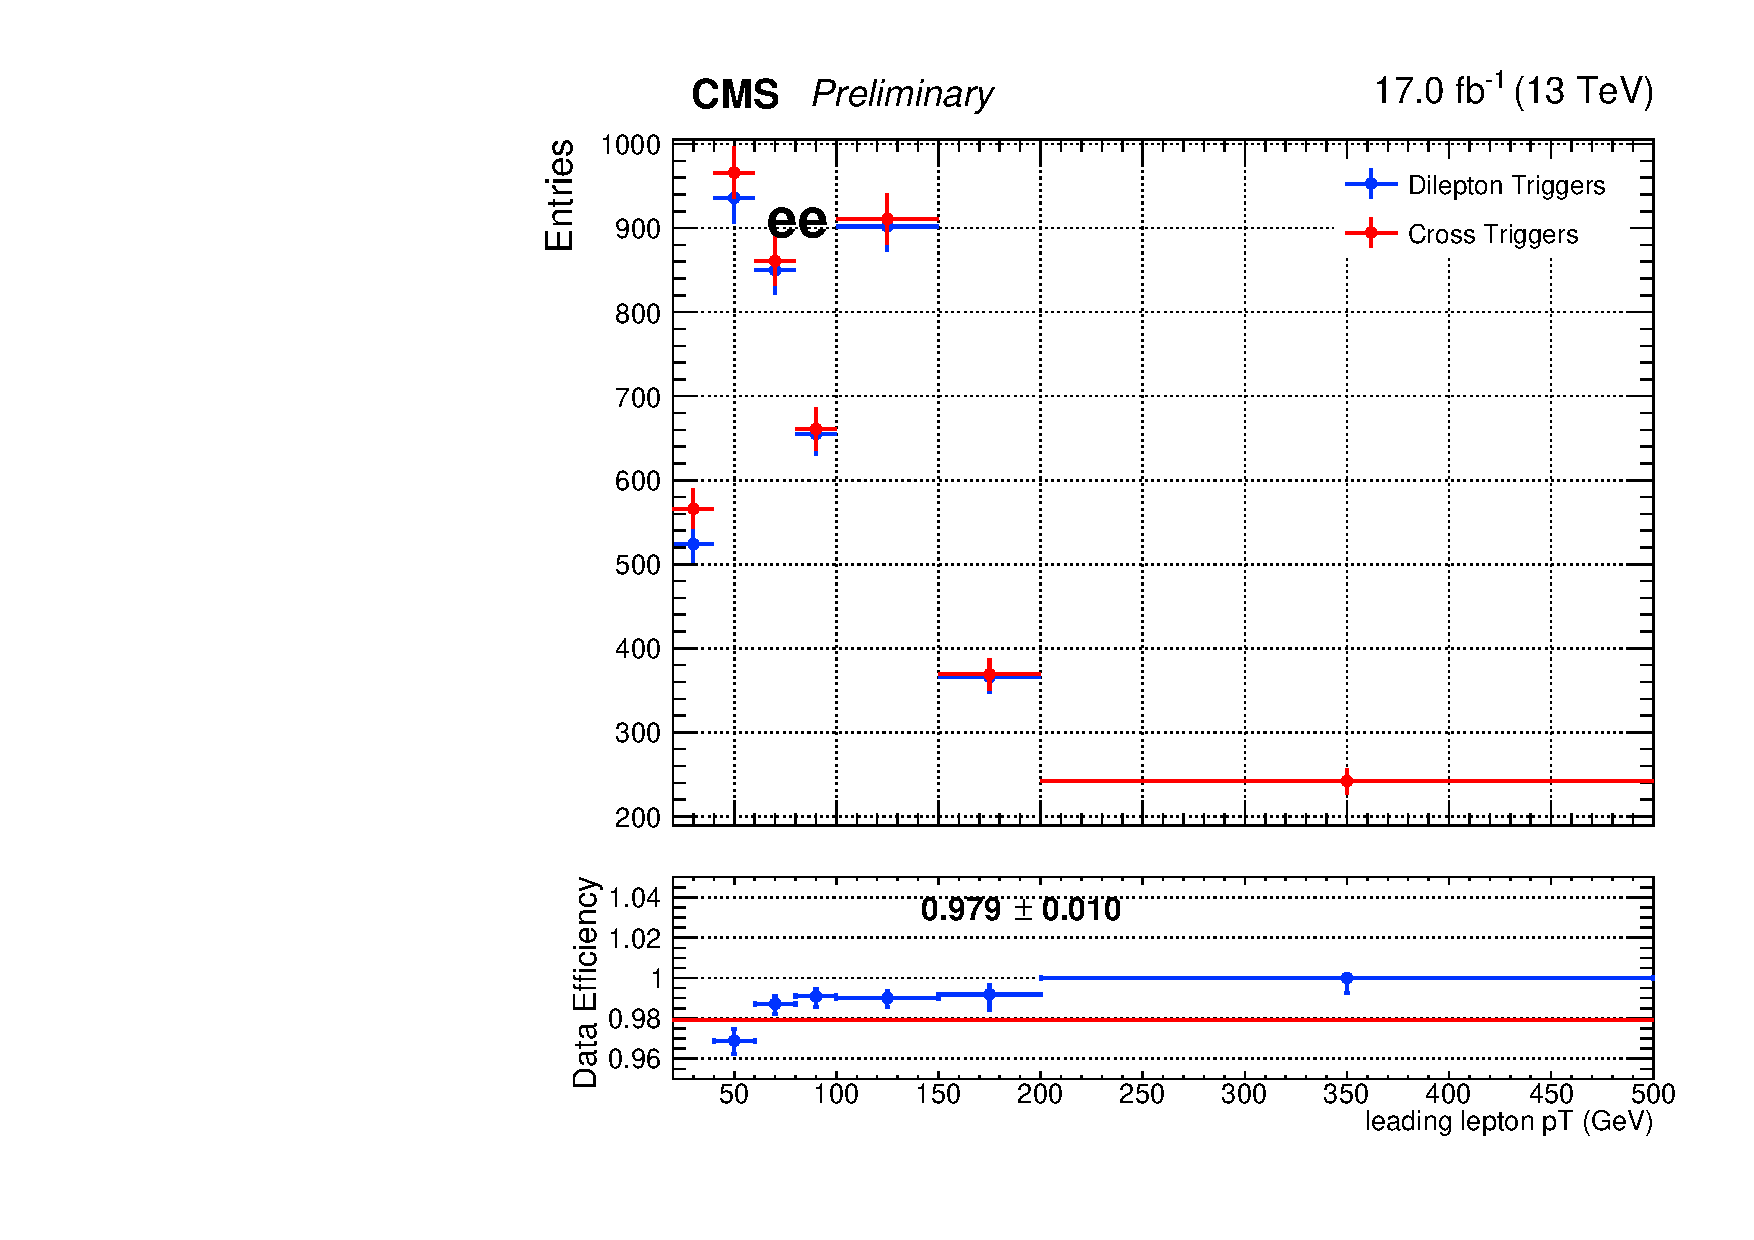
\includegraphics[width=0.32\textwidth]{fig_2016postVFP_TrigSF/g_lepApt_ee_data.pdf}
      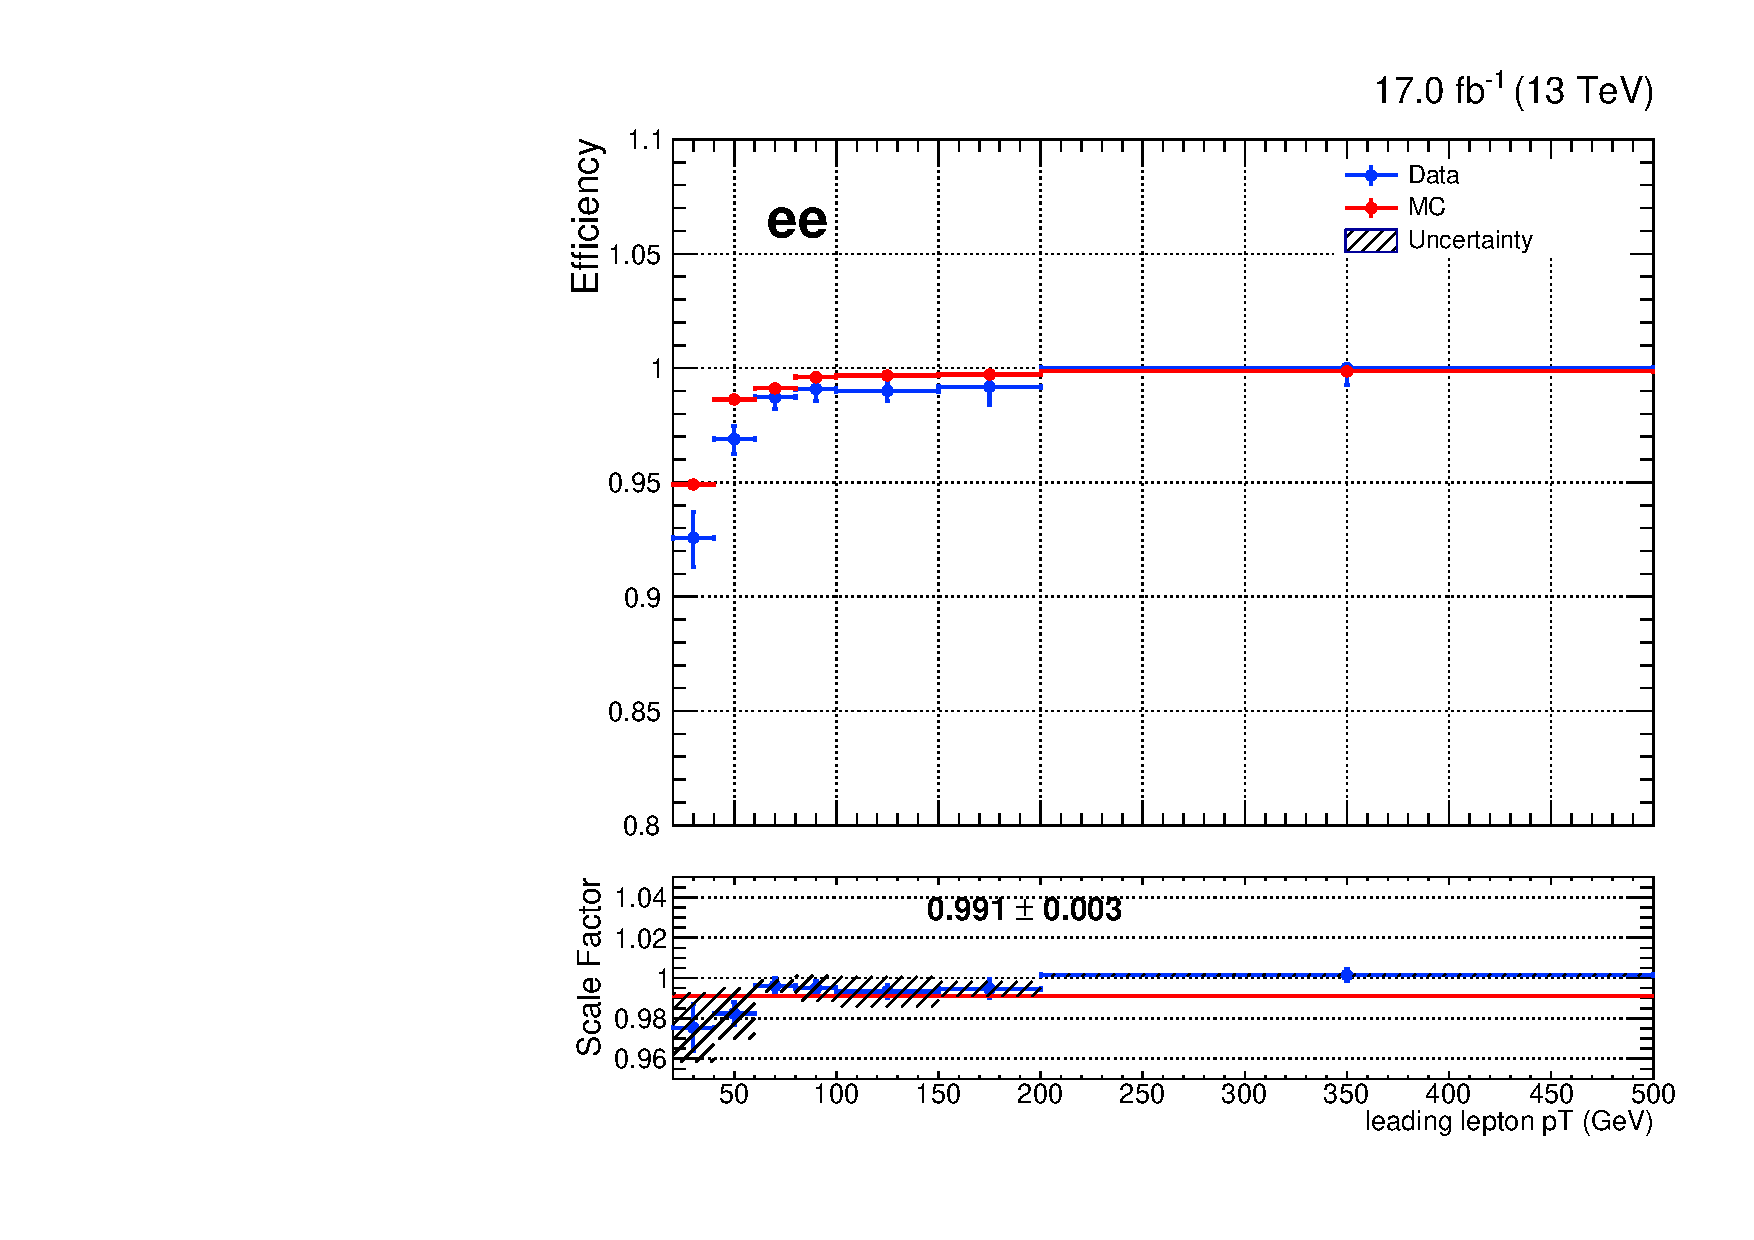
\includegraphics[width=0.32\textwidth]{fig_2016postVFP_TrigSF/g_ee_lepApt_FullSystUncBand.pdf}\\
      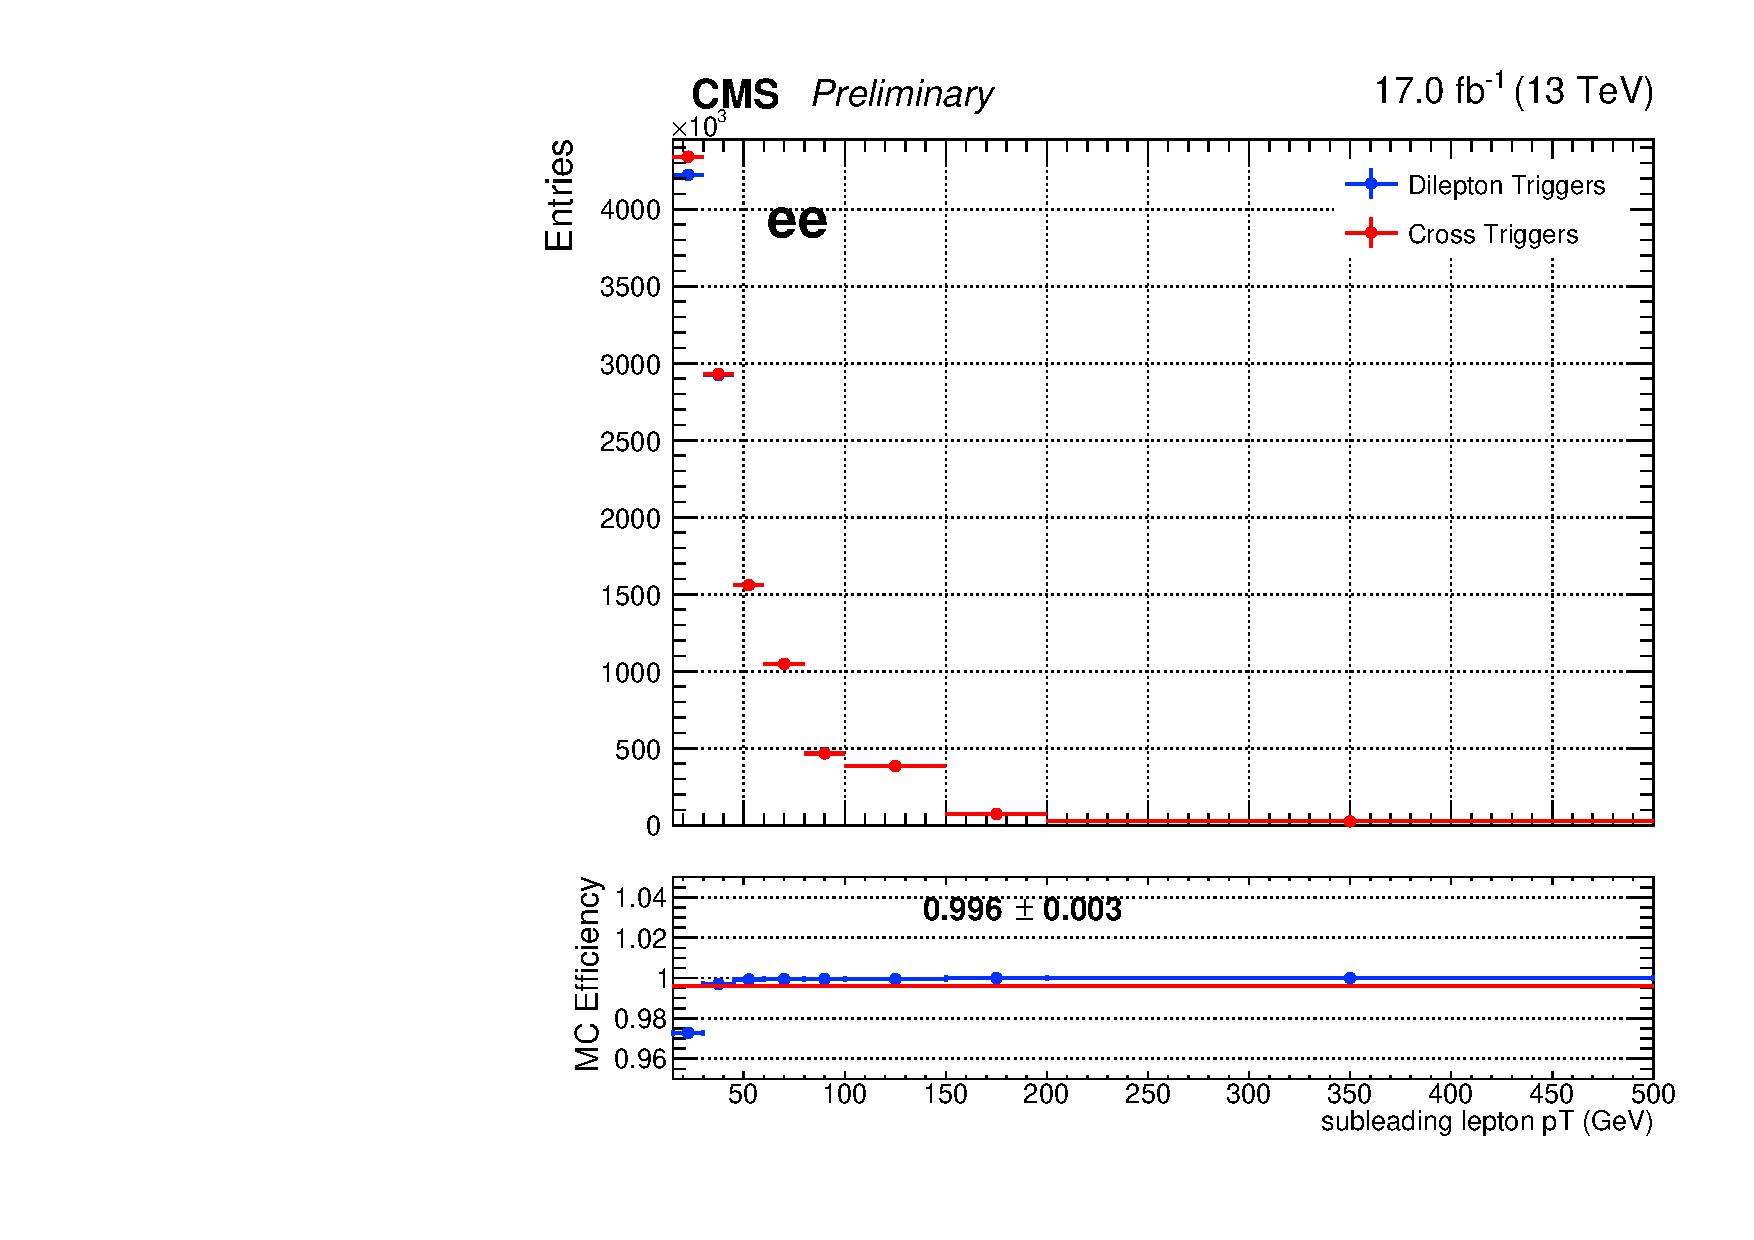
\includegraphics[width=0.32\textwidth]{fig_2016postVFP_TrigSF/g_lepBpt_ee_MC.pdf}
      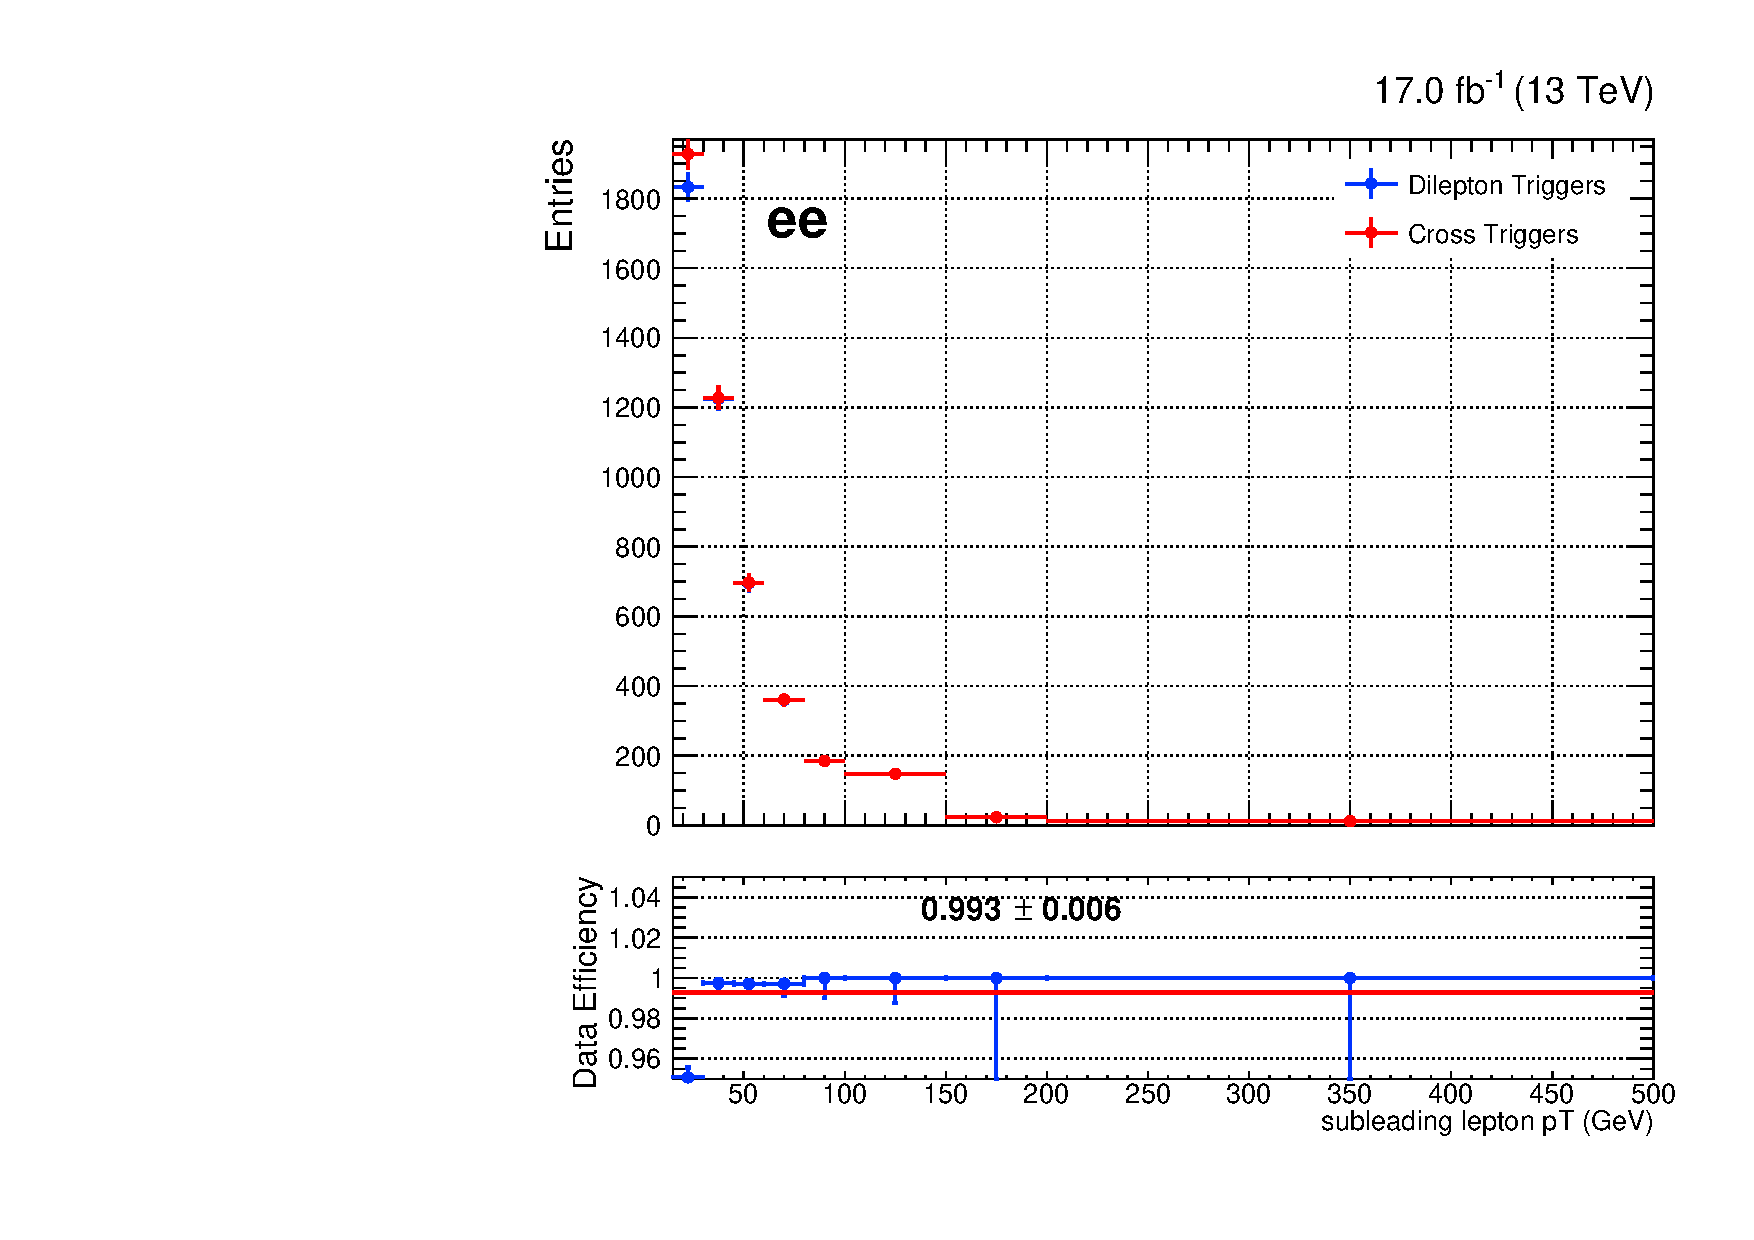
\includegraphics[width=0.32\textwidth]{fig_2016postVFP_TrigSF/g_lepBpt_ee_data.pdf}
      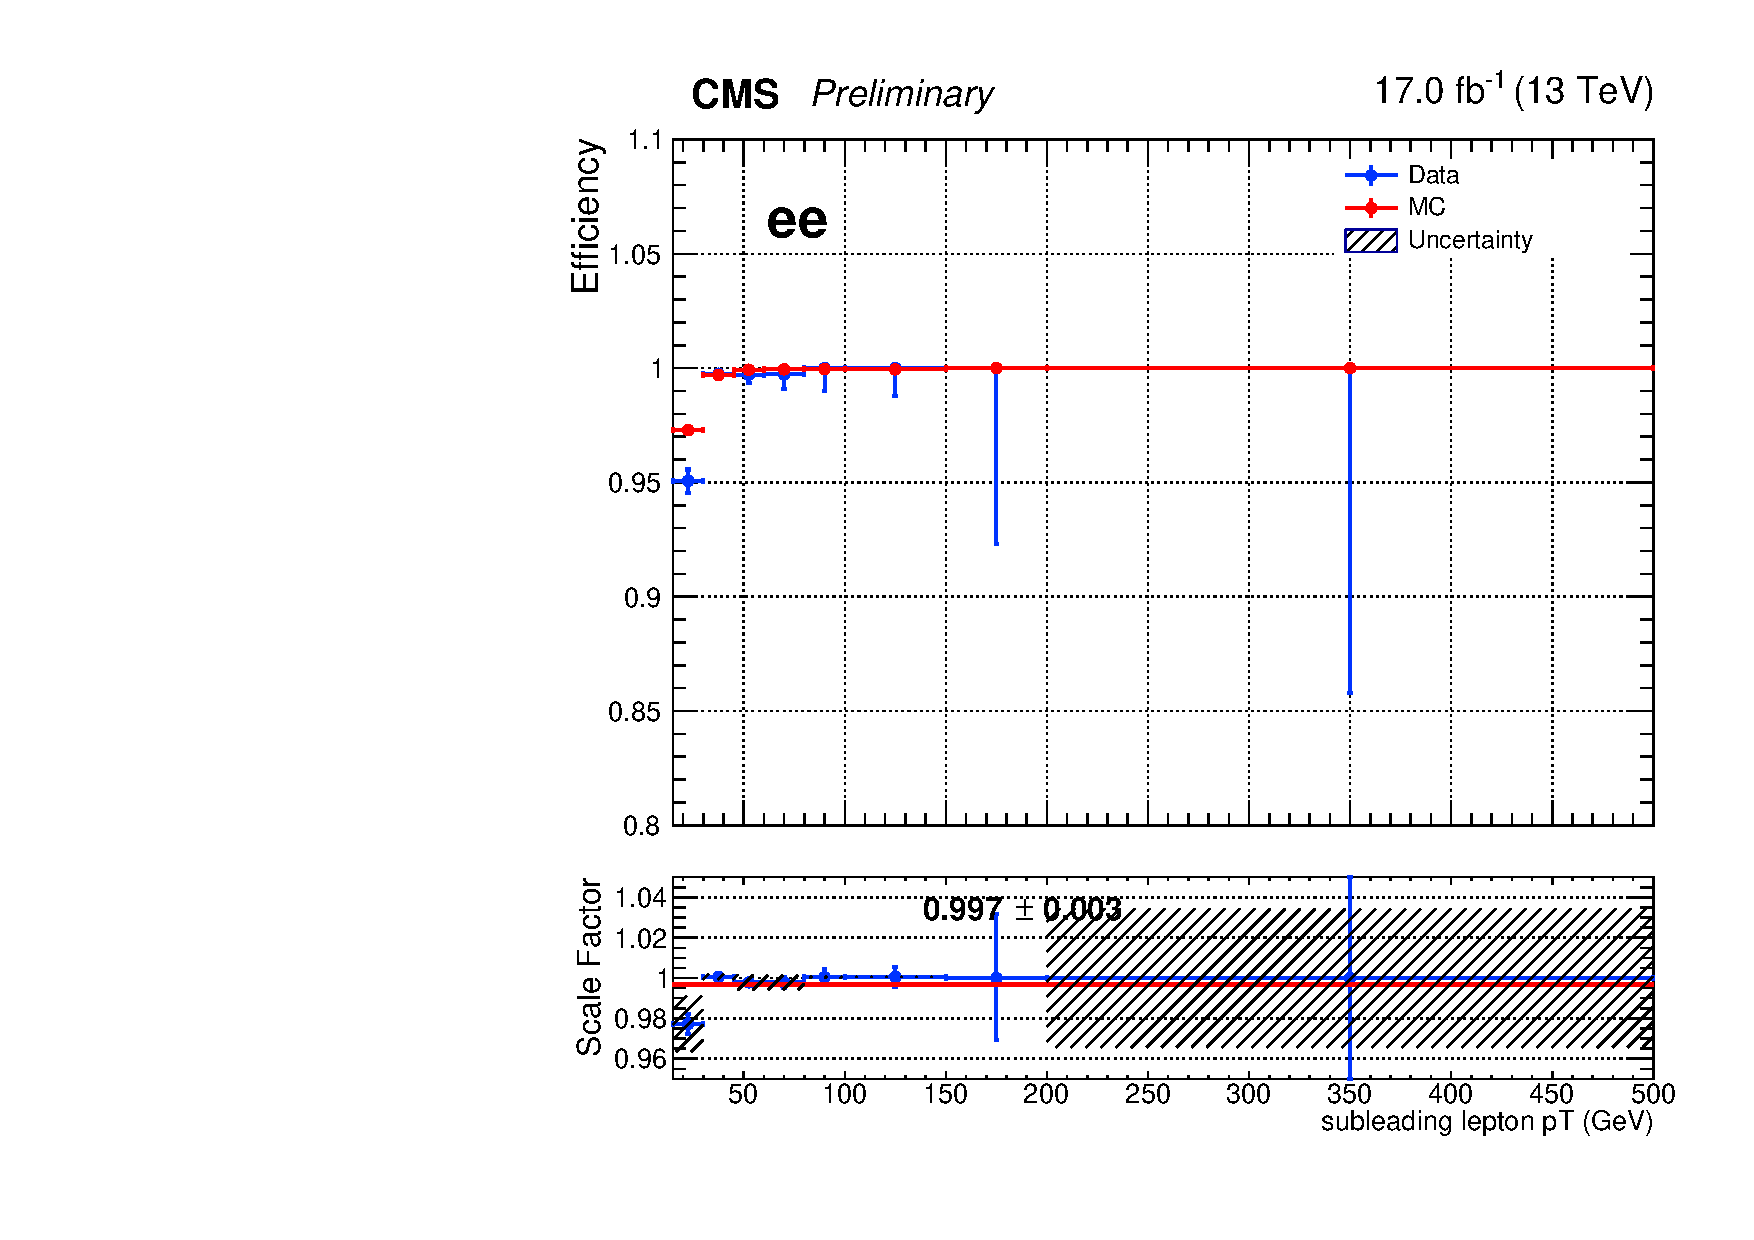
\includegraphics[width=0.32\textwidth]{fig_2016postVFP_TrigSF/g_ee_lepBpt_FullSystUncBand.pdf}\\
    \end{tabular}
    \caption{Efficiencies and scale factors for the 2016postVFP data set in the \ee channel as a function of leading and sub-leading lepton \pT.
            The error bars indicate the statistical uncertainty, and the shaded band corresponds to the systematic uncertainty.
            }
    \label{TrigSF_2016postVFP_2}
  \end{center}
\end{figure}

\begin{figure}[h]
  \begin{center}
    \begin{tabular}{ccc}
      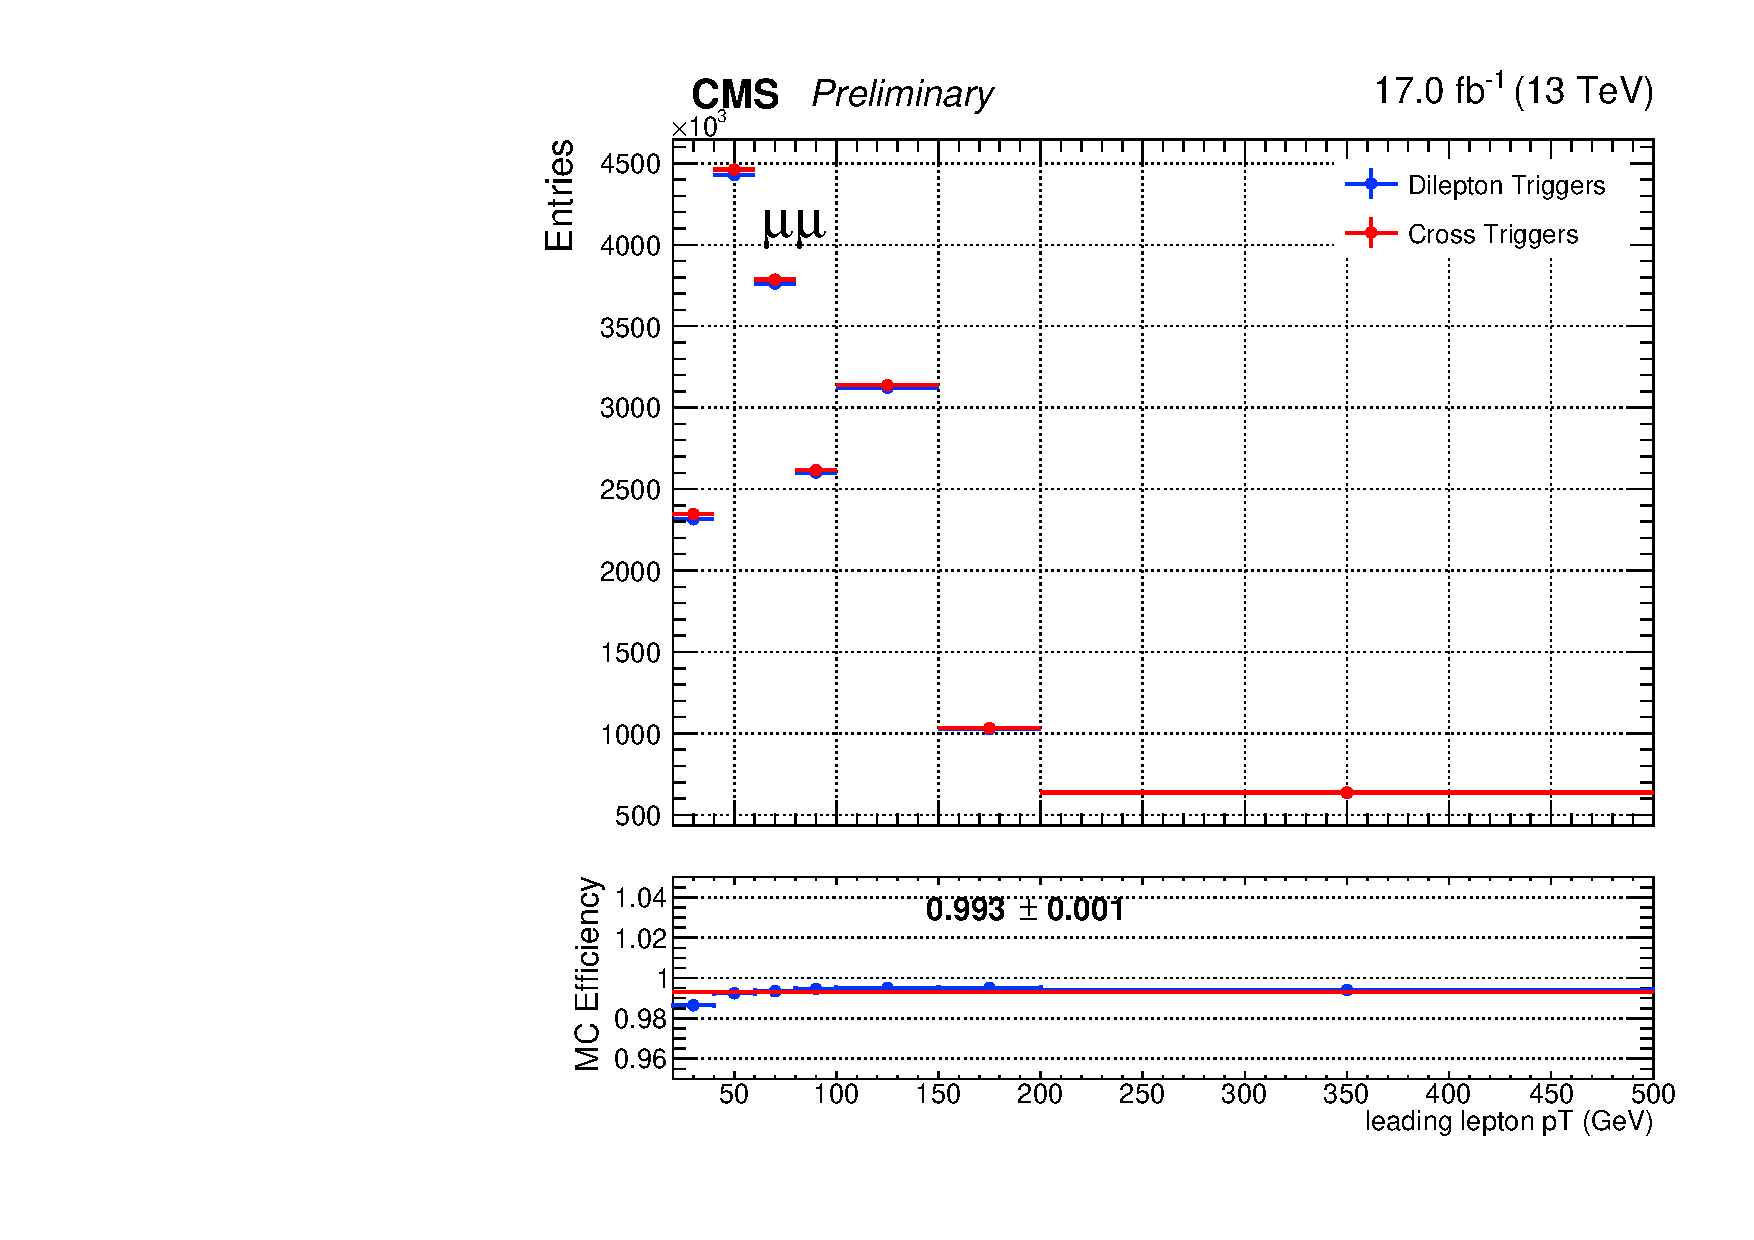
\includegraphics[width=0.32\textwidth]{fig_2016postVFP_TrigSF/g_lepApt_mumu_MC.pdf}
      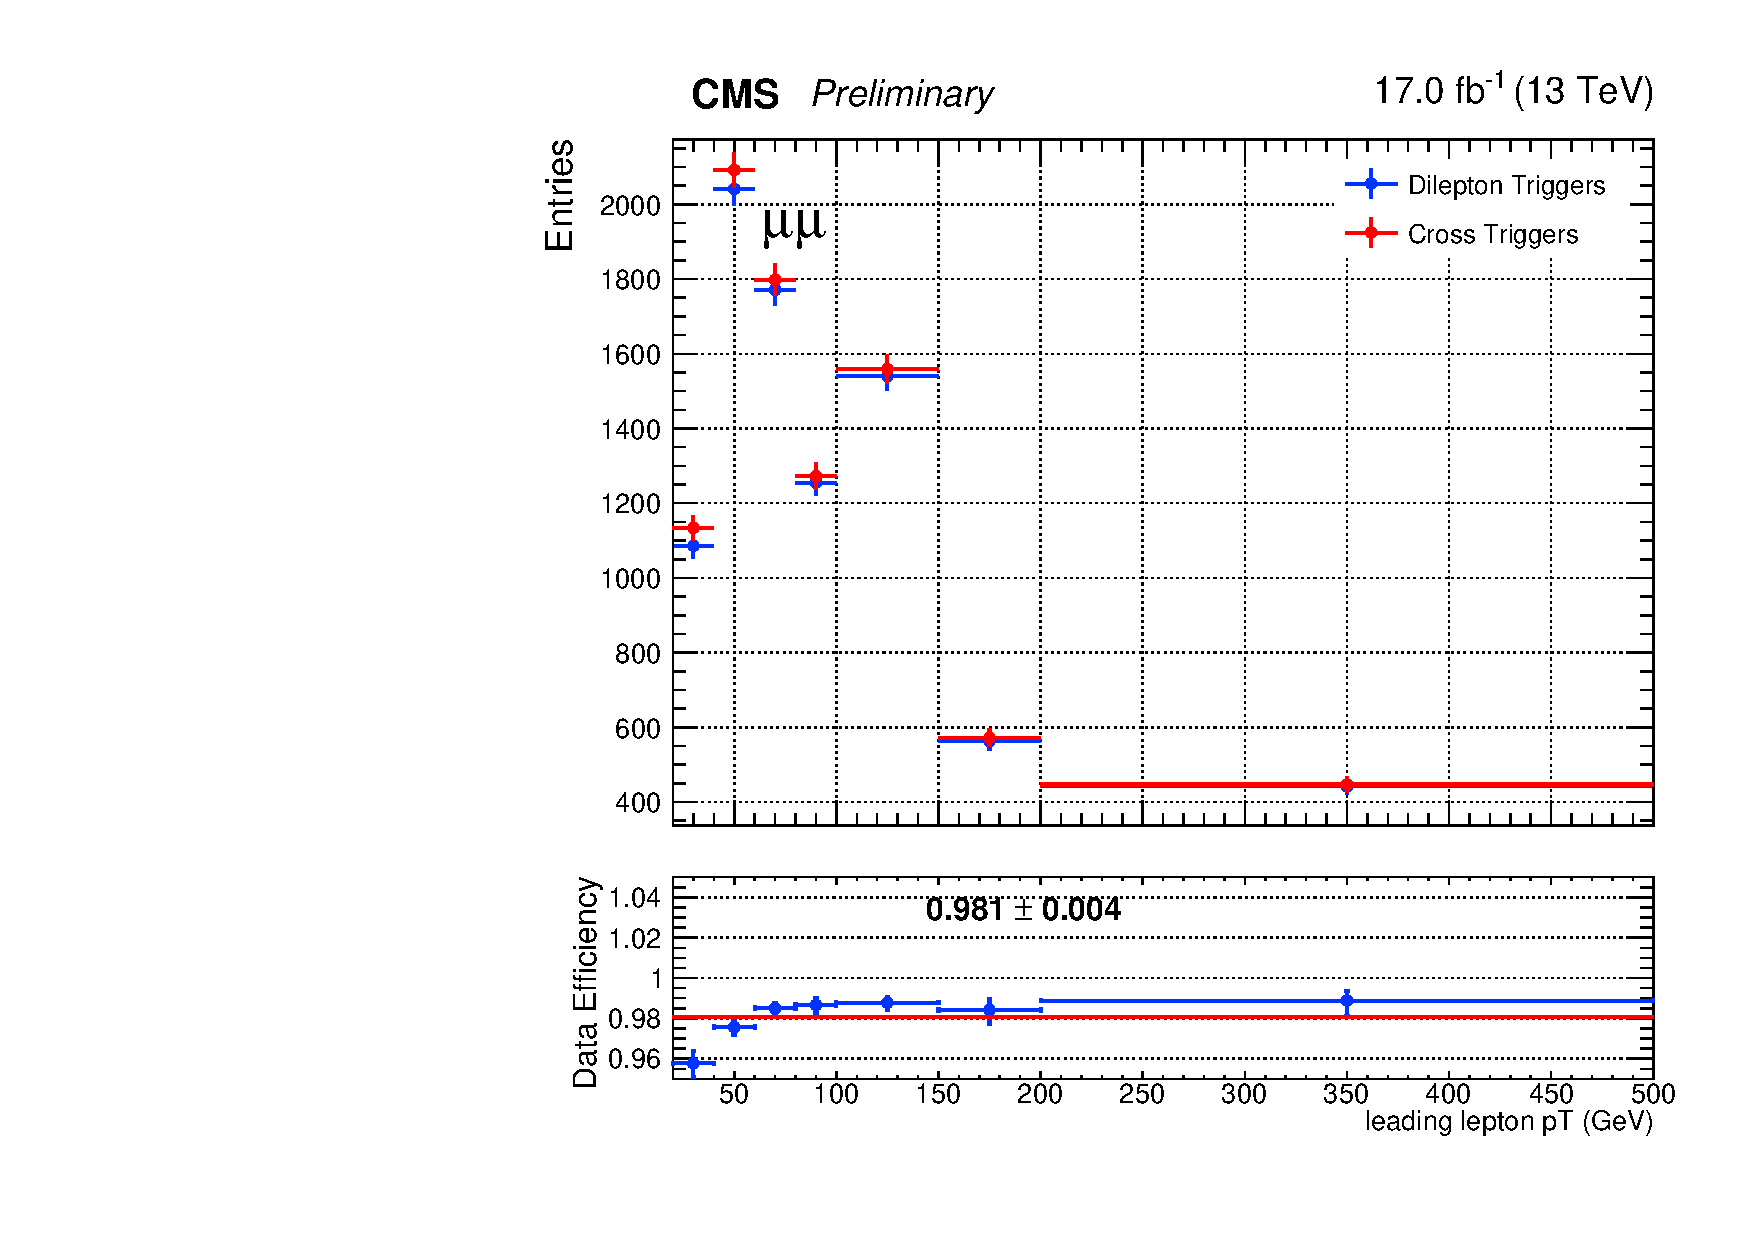
\includegraphics[width=0.32\textwidth]{fig_2016postVFP_TrigSF/g_lepApt_mumu_data.pdf}
      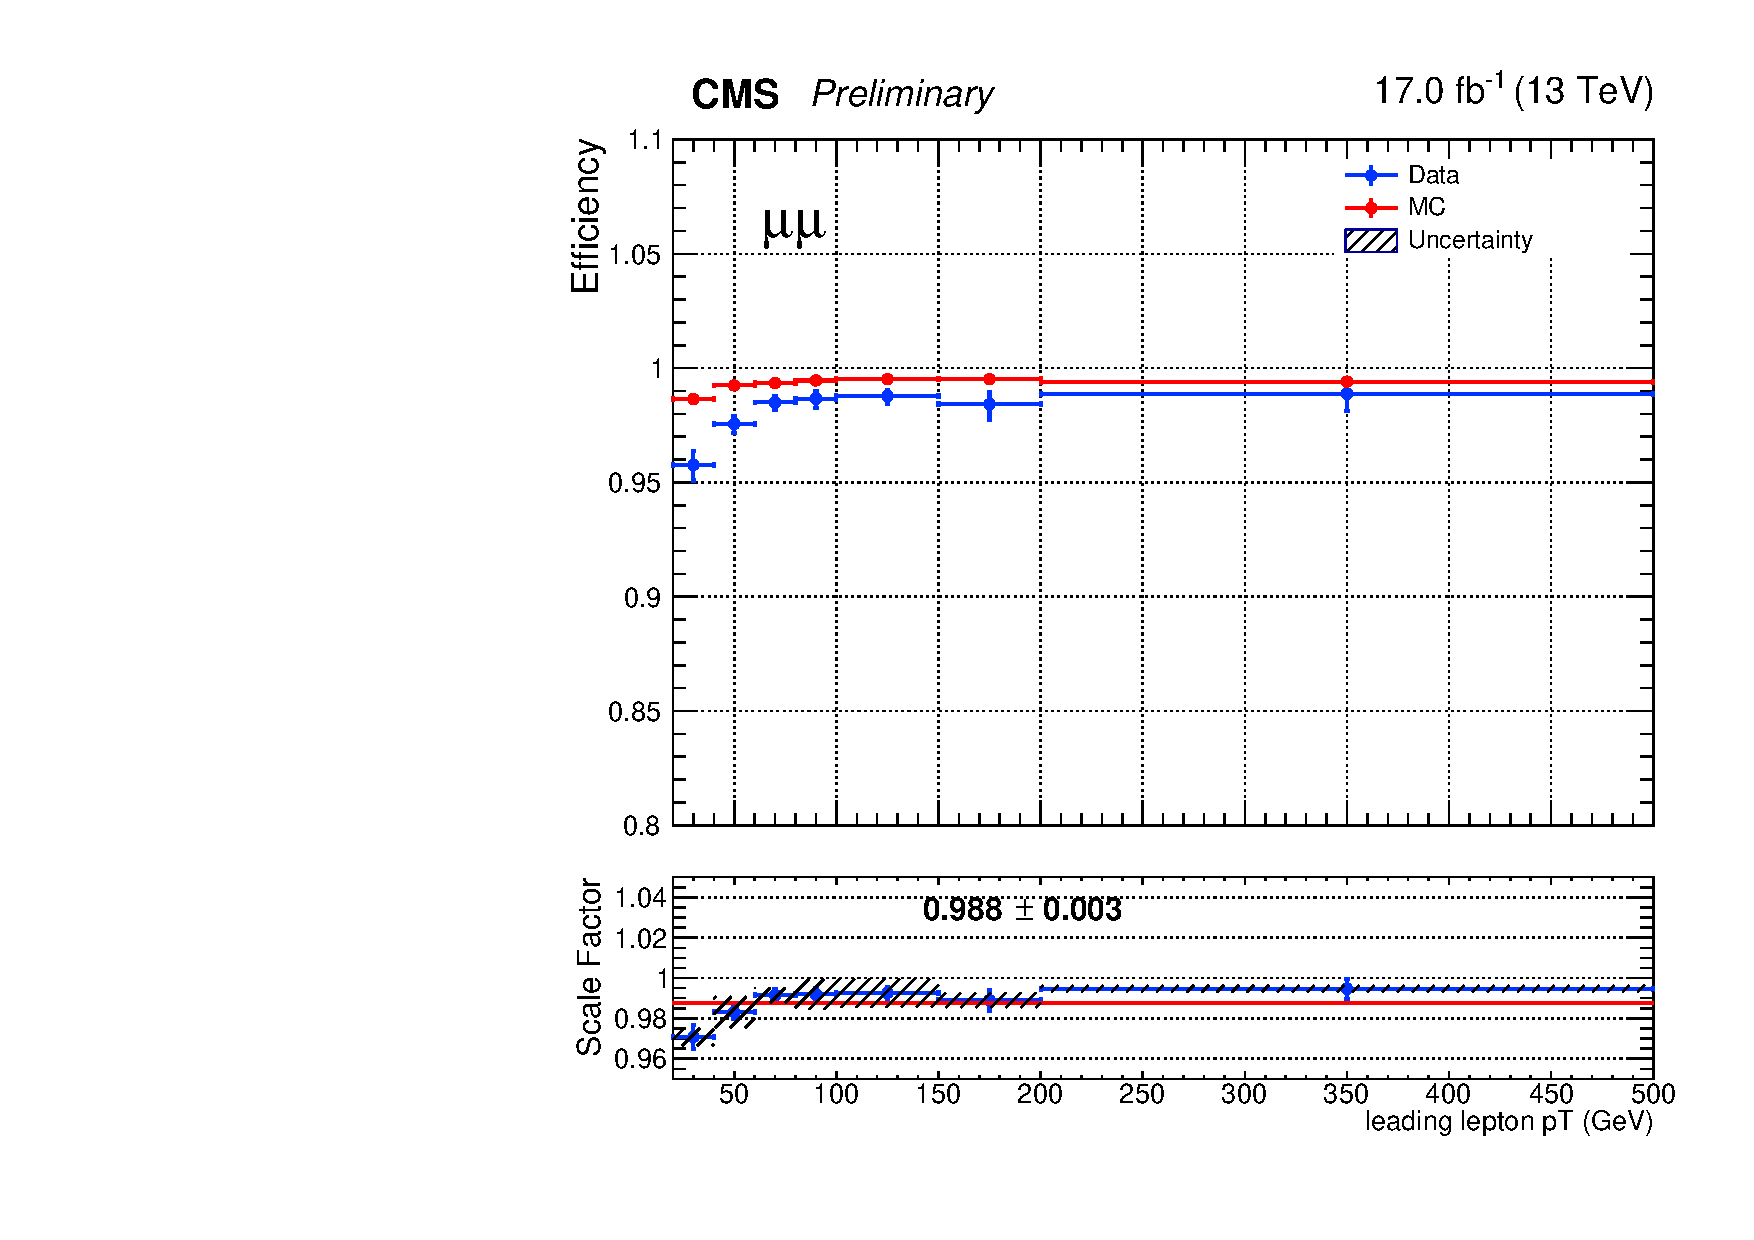
\includegraphics[width=0.32\textwidth]{fig_2016postVFP_TrigSF/g_mumu_lepApt_FullSystUncBand.pdf}\\
      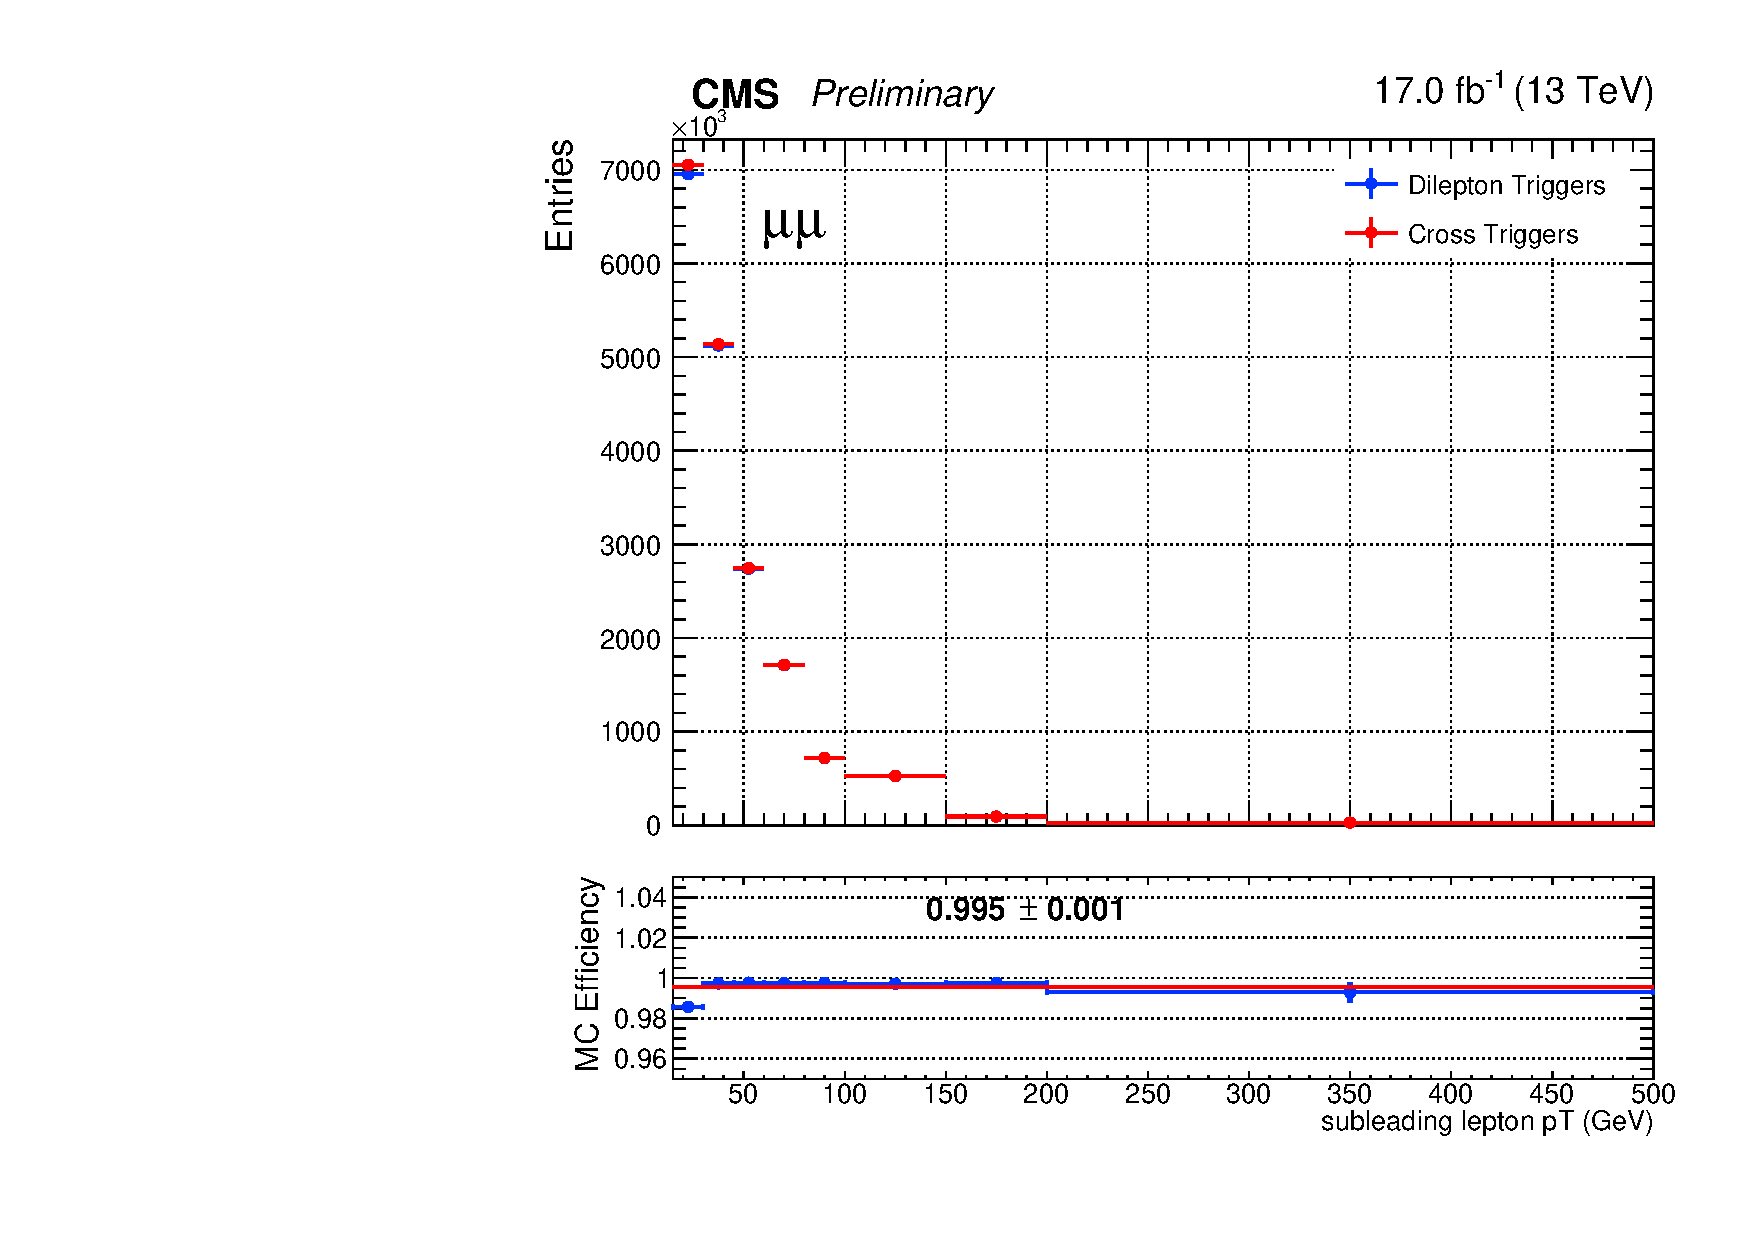
\includegraphics[width=0.32\textwidth]{fig_2016postVFP_TrigSF/g_lepBpt_mumu_MC.pdf}
      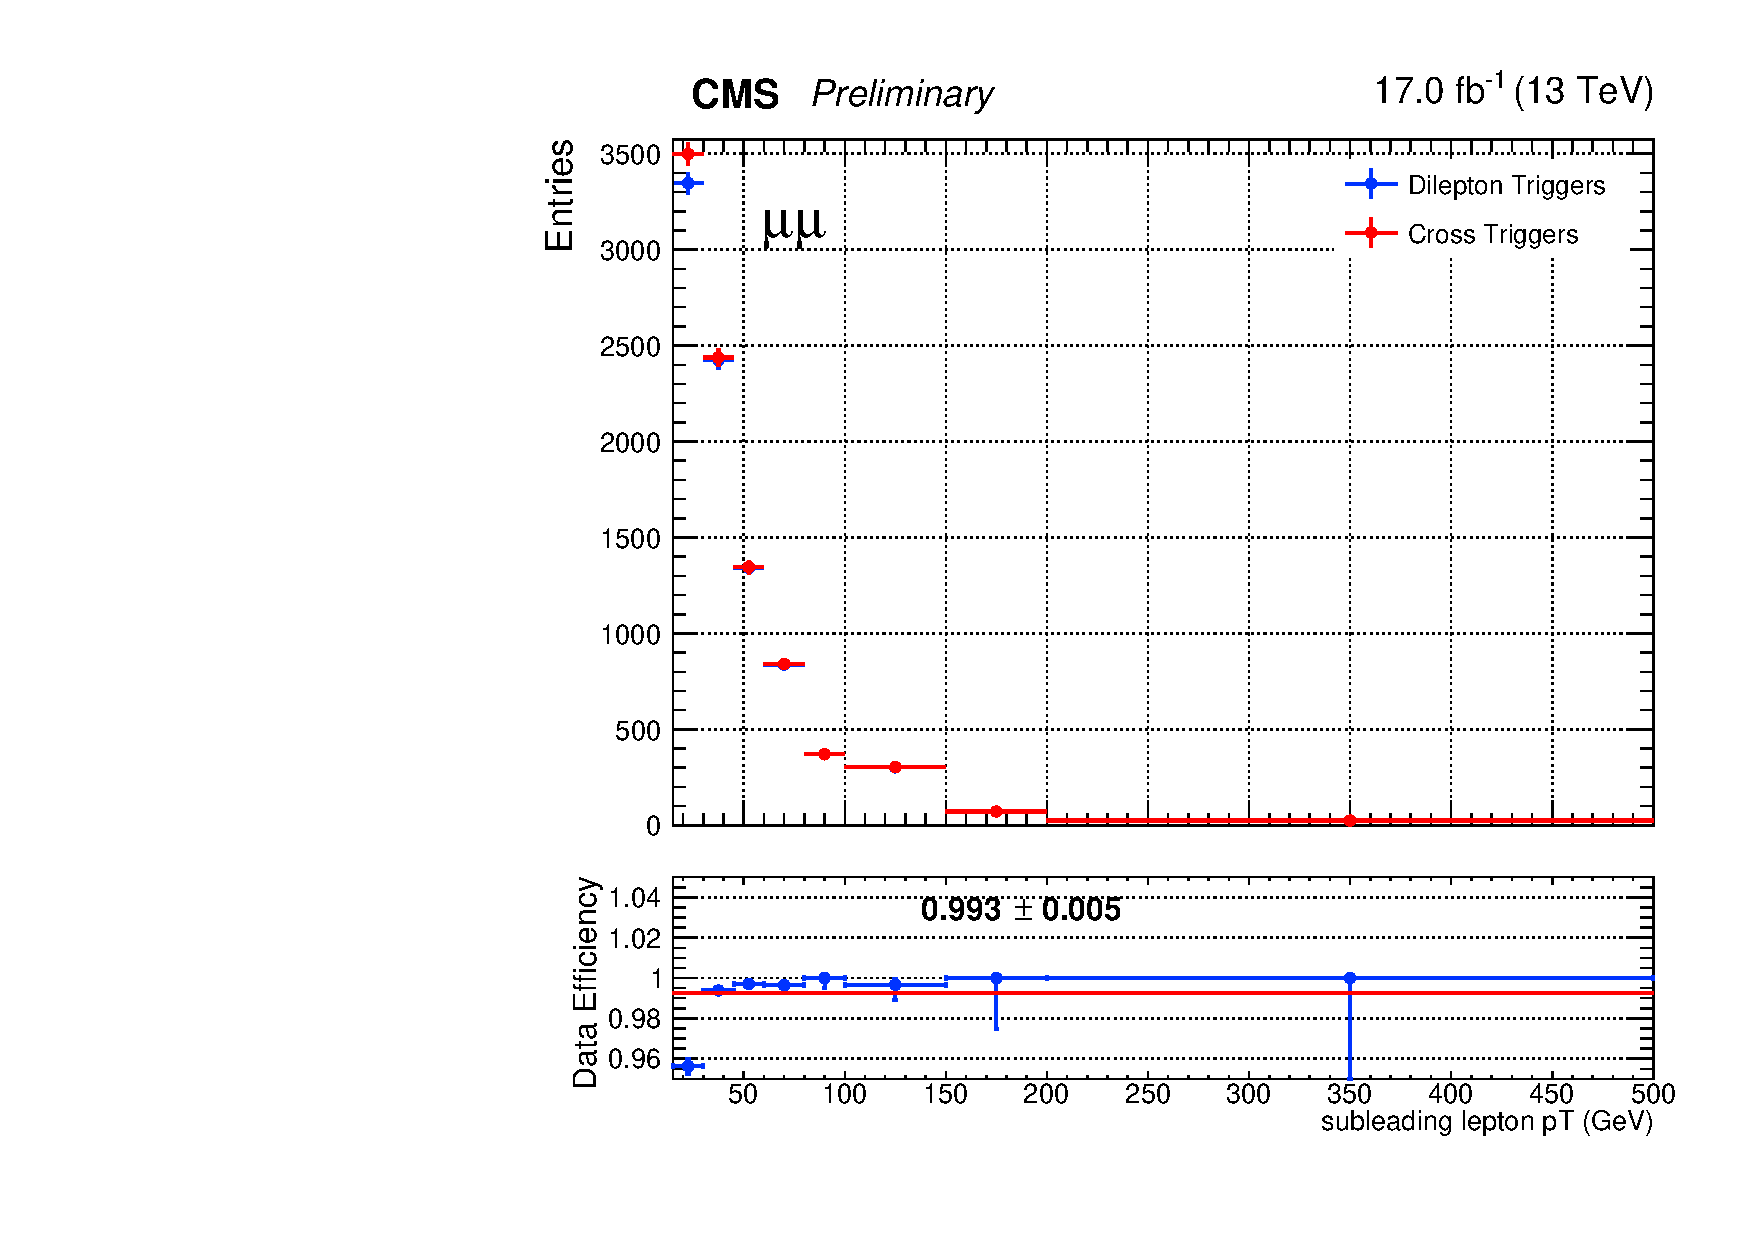
\includegraphics[width=0.32\textwidth]{fig_2016postVFP_TrigSF/g_lepBpt_mumu_data.pdf}
      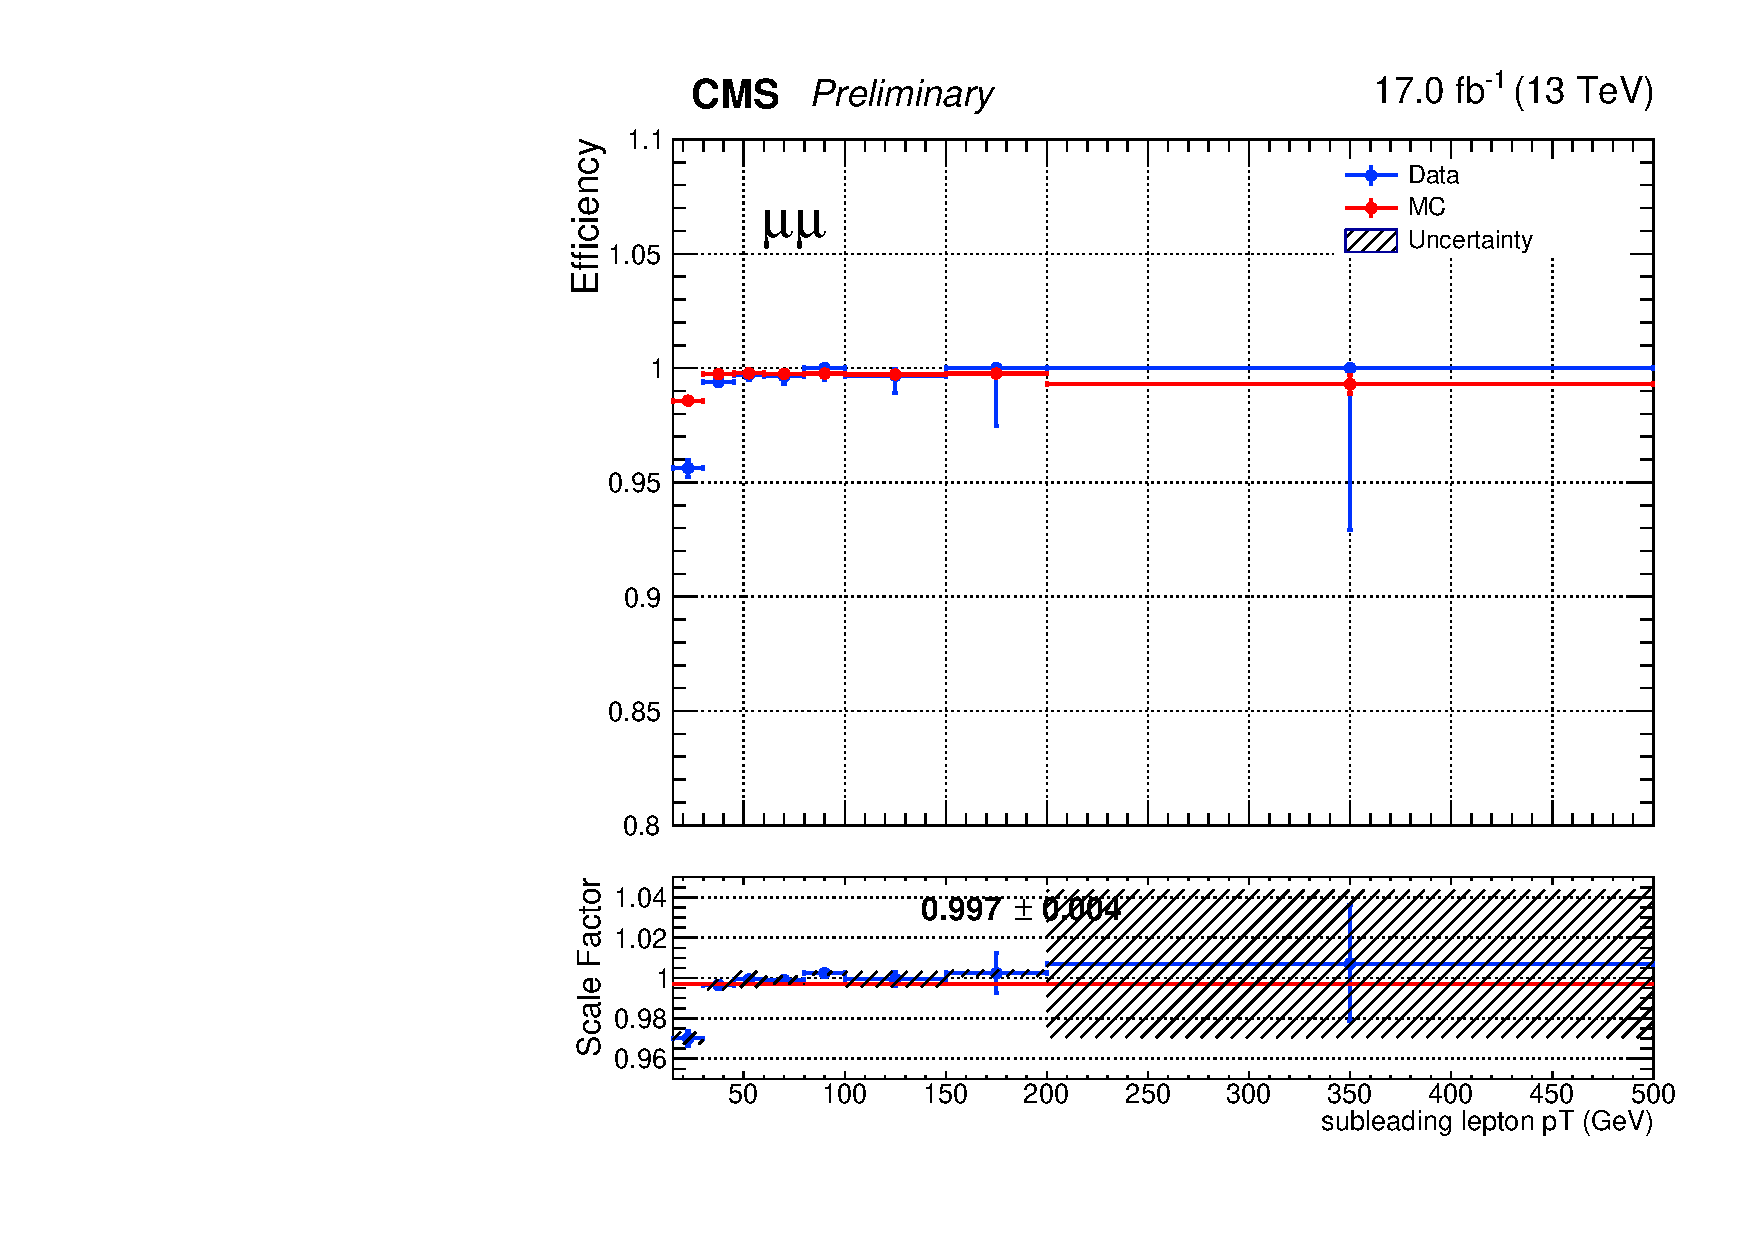
\includegraphics[width=0.32\textwidth]{fig_2016postVFP_TrigSF/g_mumu_lepBpt_FullSystUncBand.pdf}\\
    \end{tabular}
    \caption{Efficiencies and scale factors for the 2016postVFP data set in the \mumu channel as a function of leading and sub-leading lepton \pT.
            The error bars indicate the statistical uncertainty, and the shaded band corresponds to the systematic uncertainty.
            }
    \label{TrigSF_2016postVFP_3}
  \end{center}
\end{figure}

\begin{figure}[h]
  \begin{center}
    \begin{tabular}{cc}
      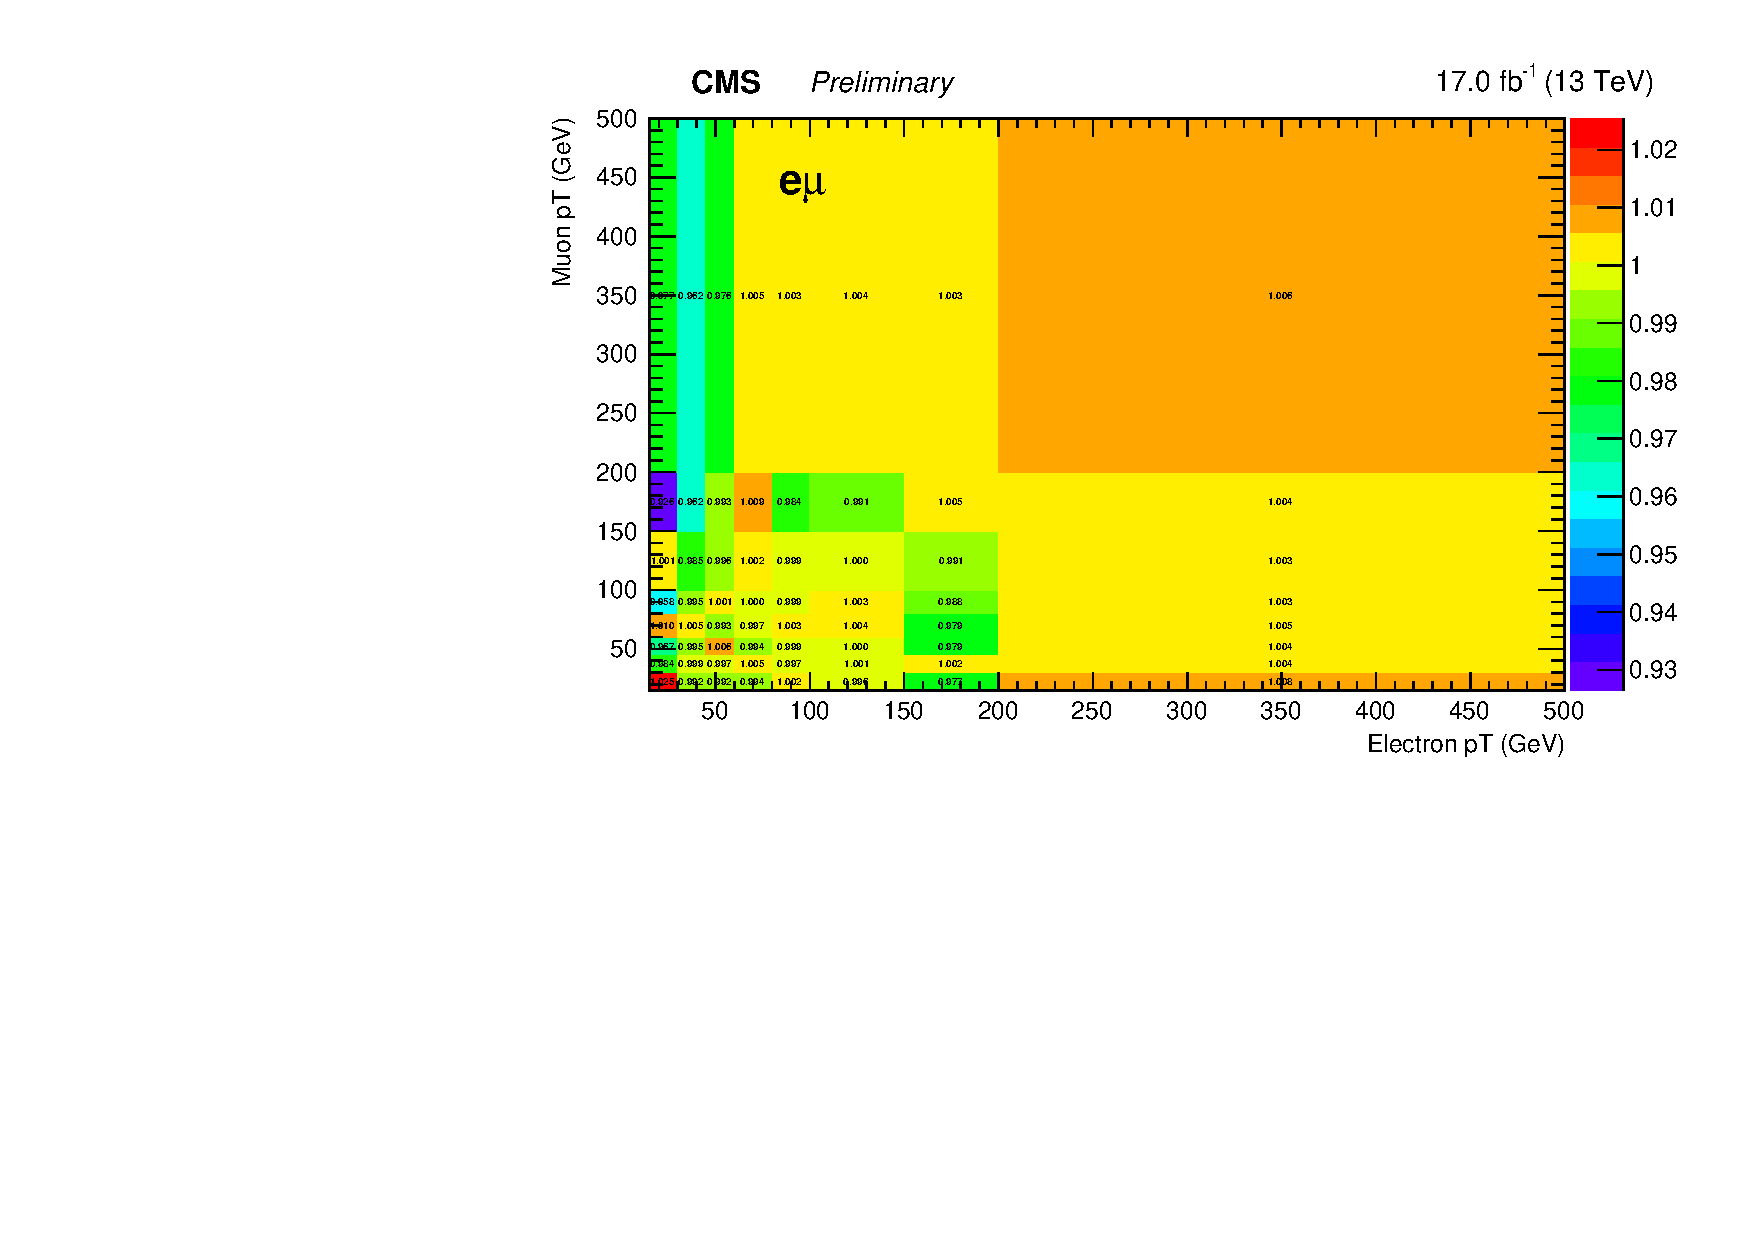
\includegraphics[width=0.50\textwidth]{fig_2016postVFP_TrigSF/h2D_lepABpt_emu.pdf}
      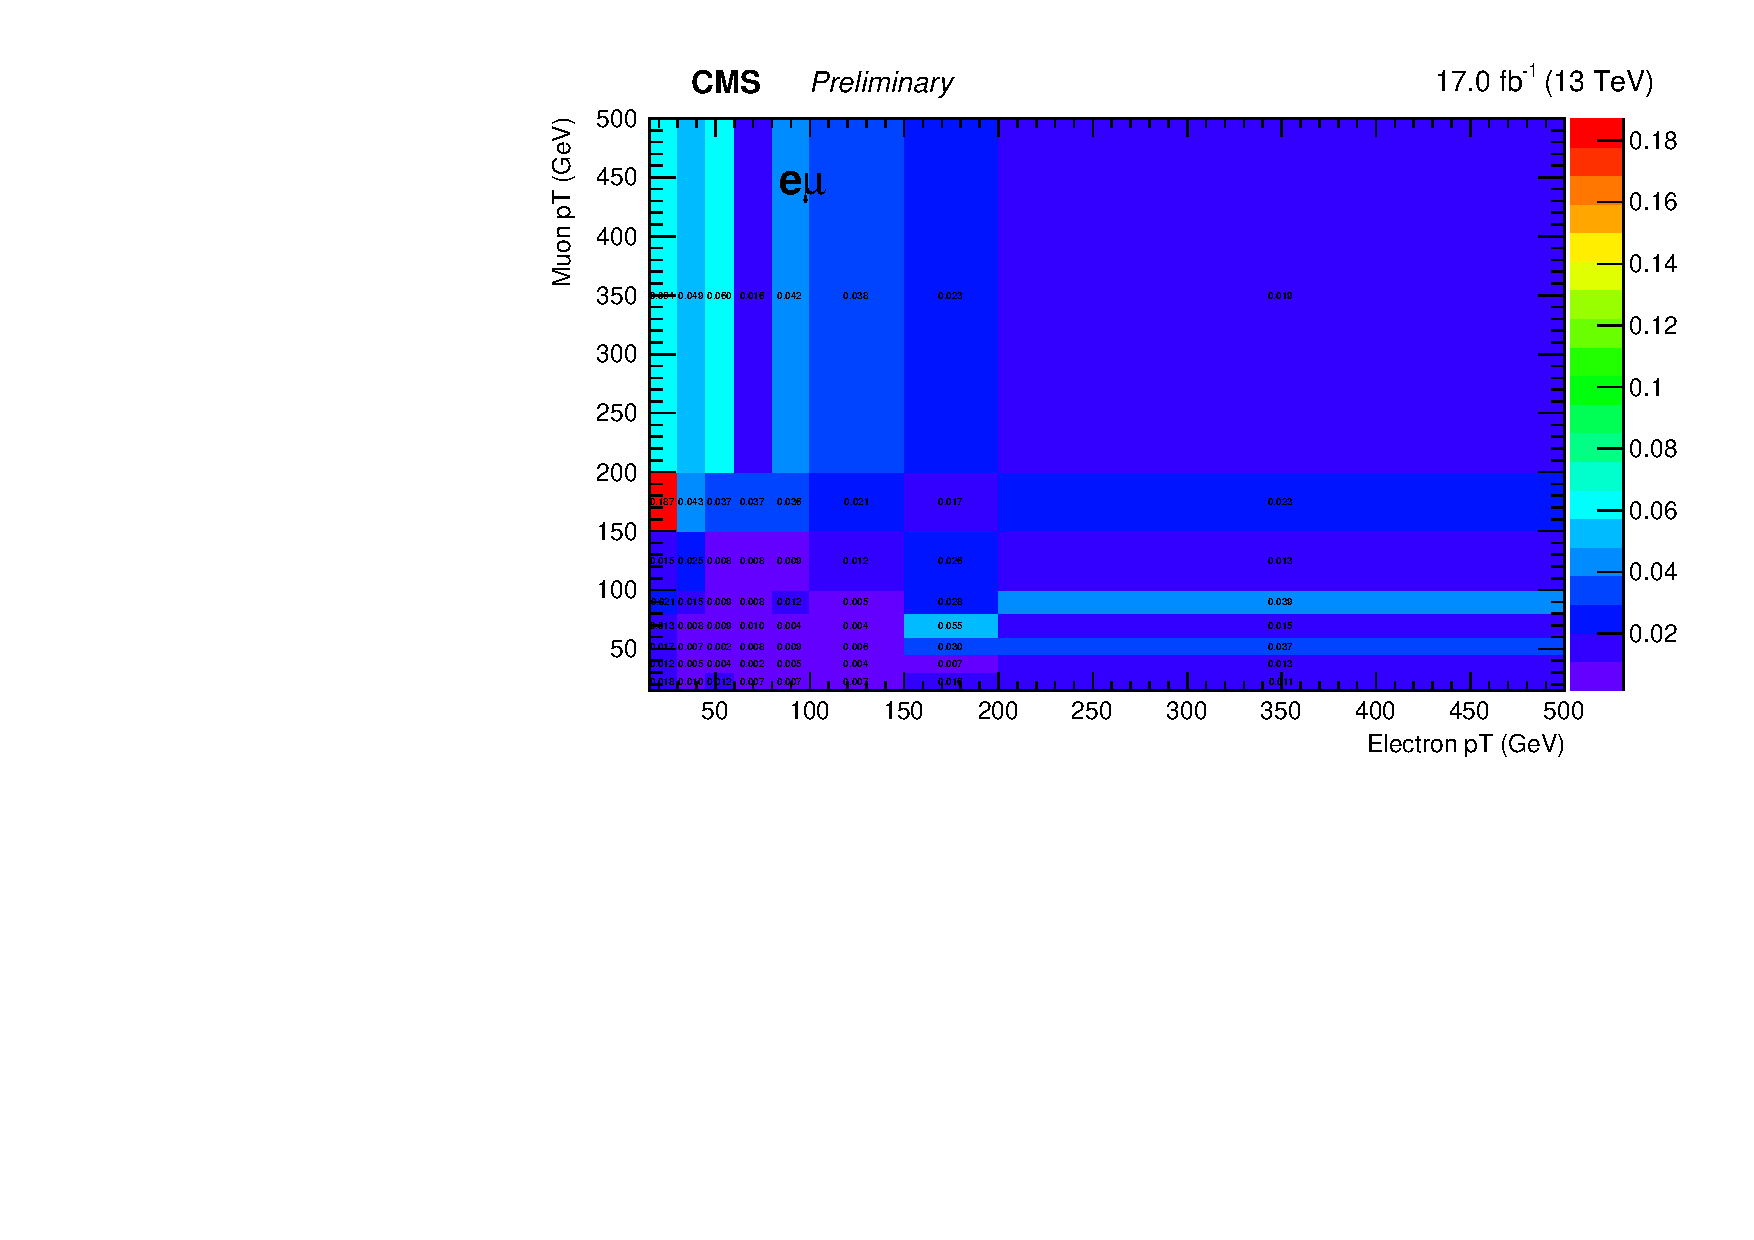
\includegraphics[width=0.50\textwidth]{fig_2016postVFP_TrigSF/h2D_lepABpt_emu_BinErrors.pdf}\\       
      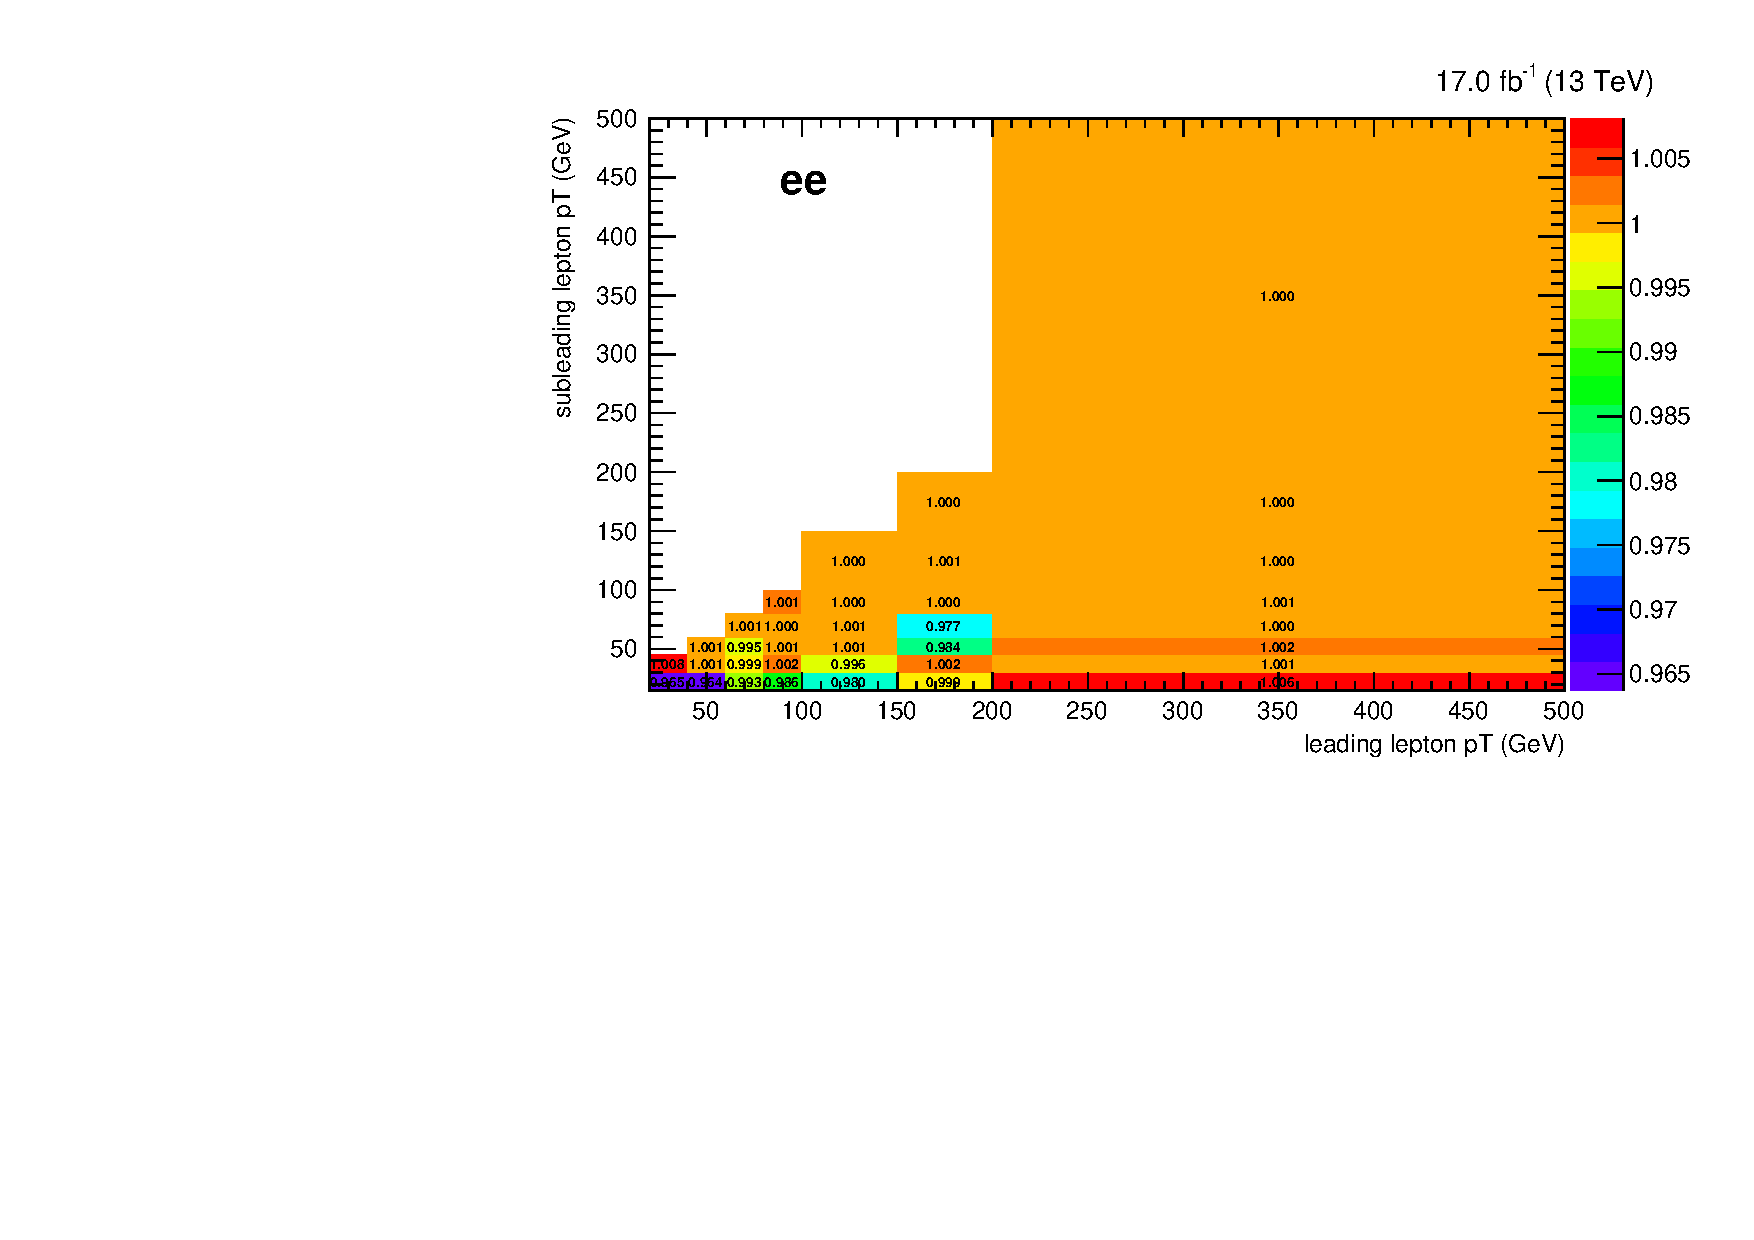
\includegraphics[width=0.50\textwidth]{fig_2016postVFP_TrigSF/h2D_lepABpt_ee.pdf}
      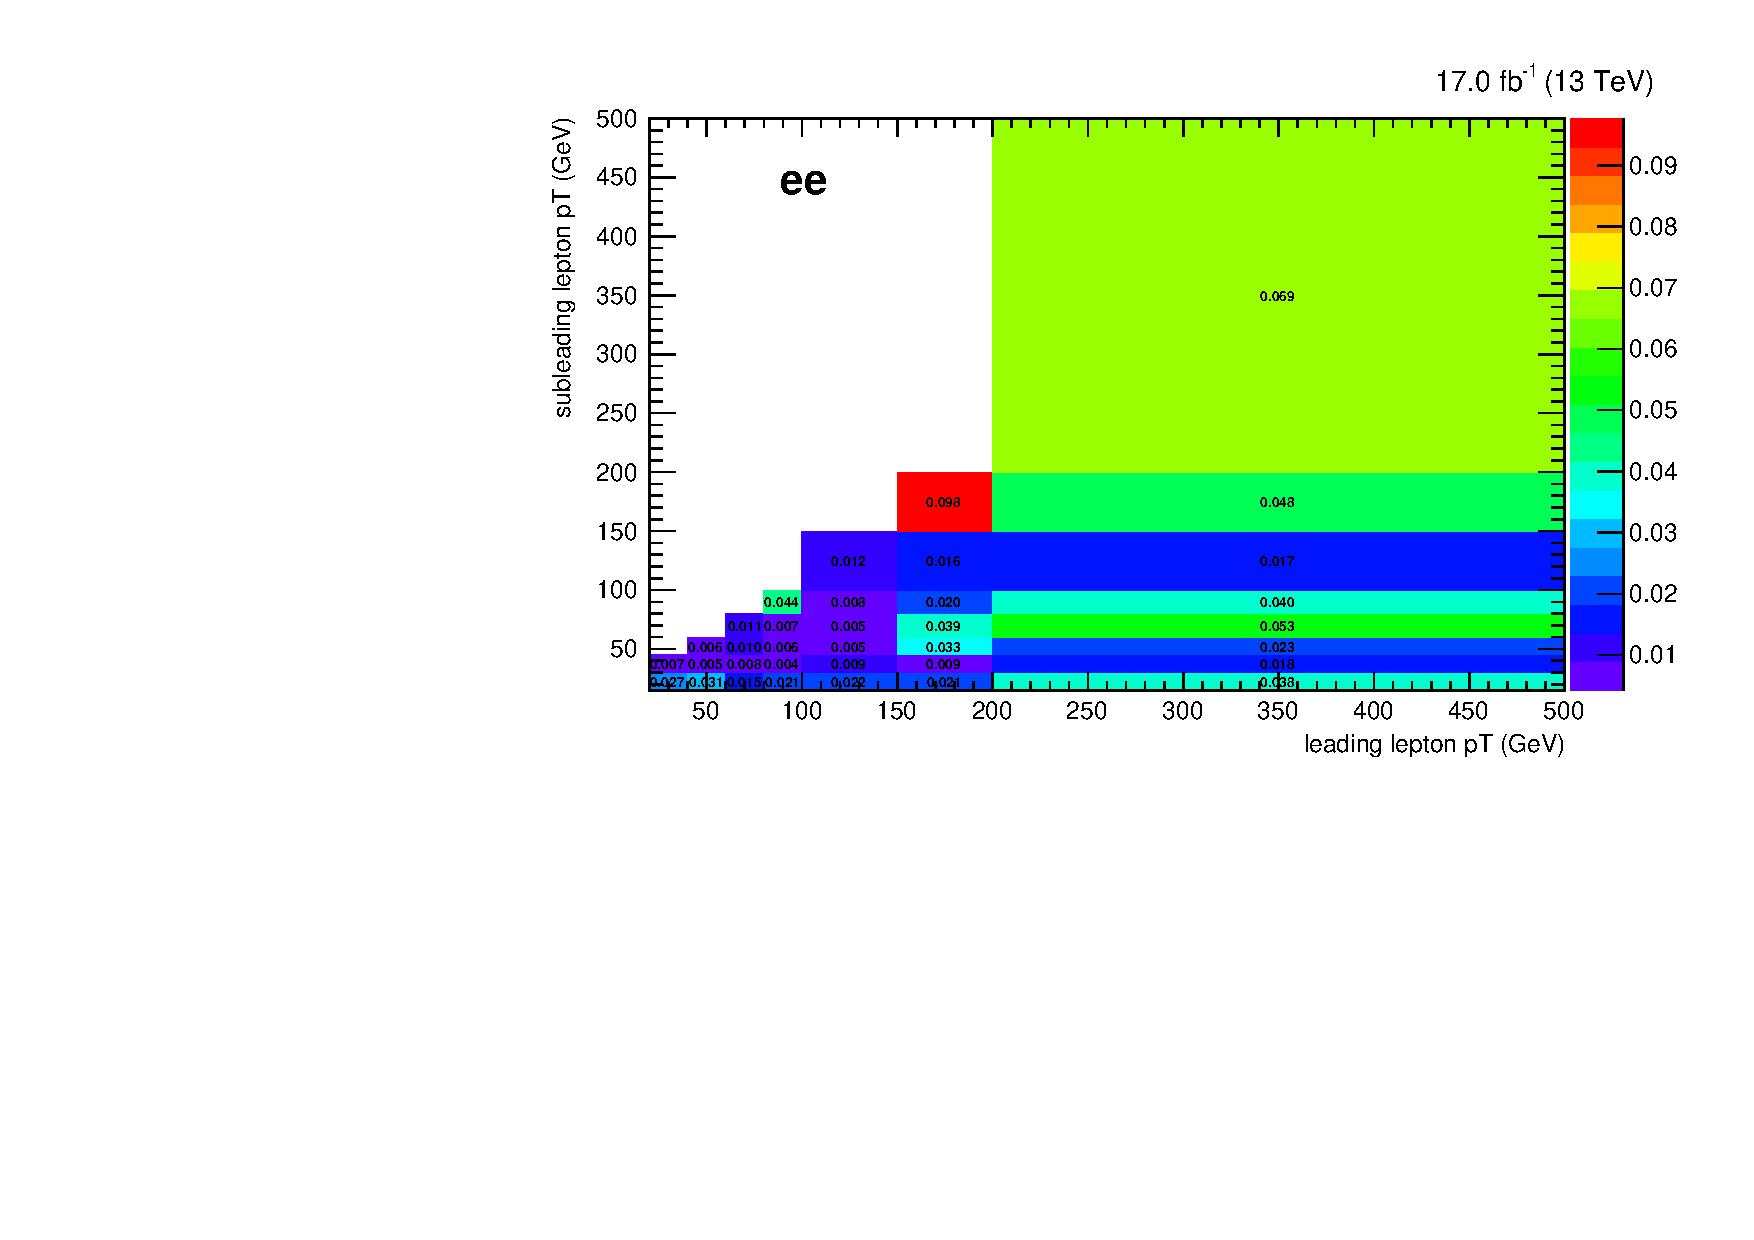
\includegraphics[width=0.50\textwidth]{fig_2016postVFP_TrigSF/h2D_lepABpt_ee_BinErrors.pdf}\\
      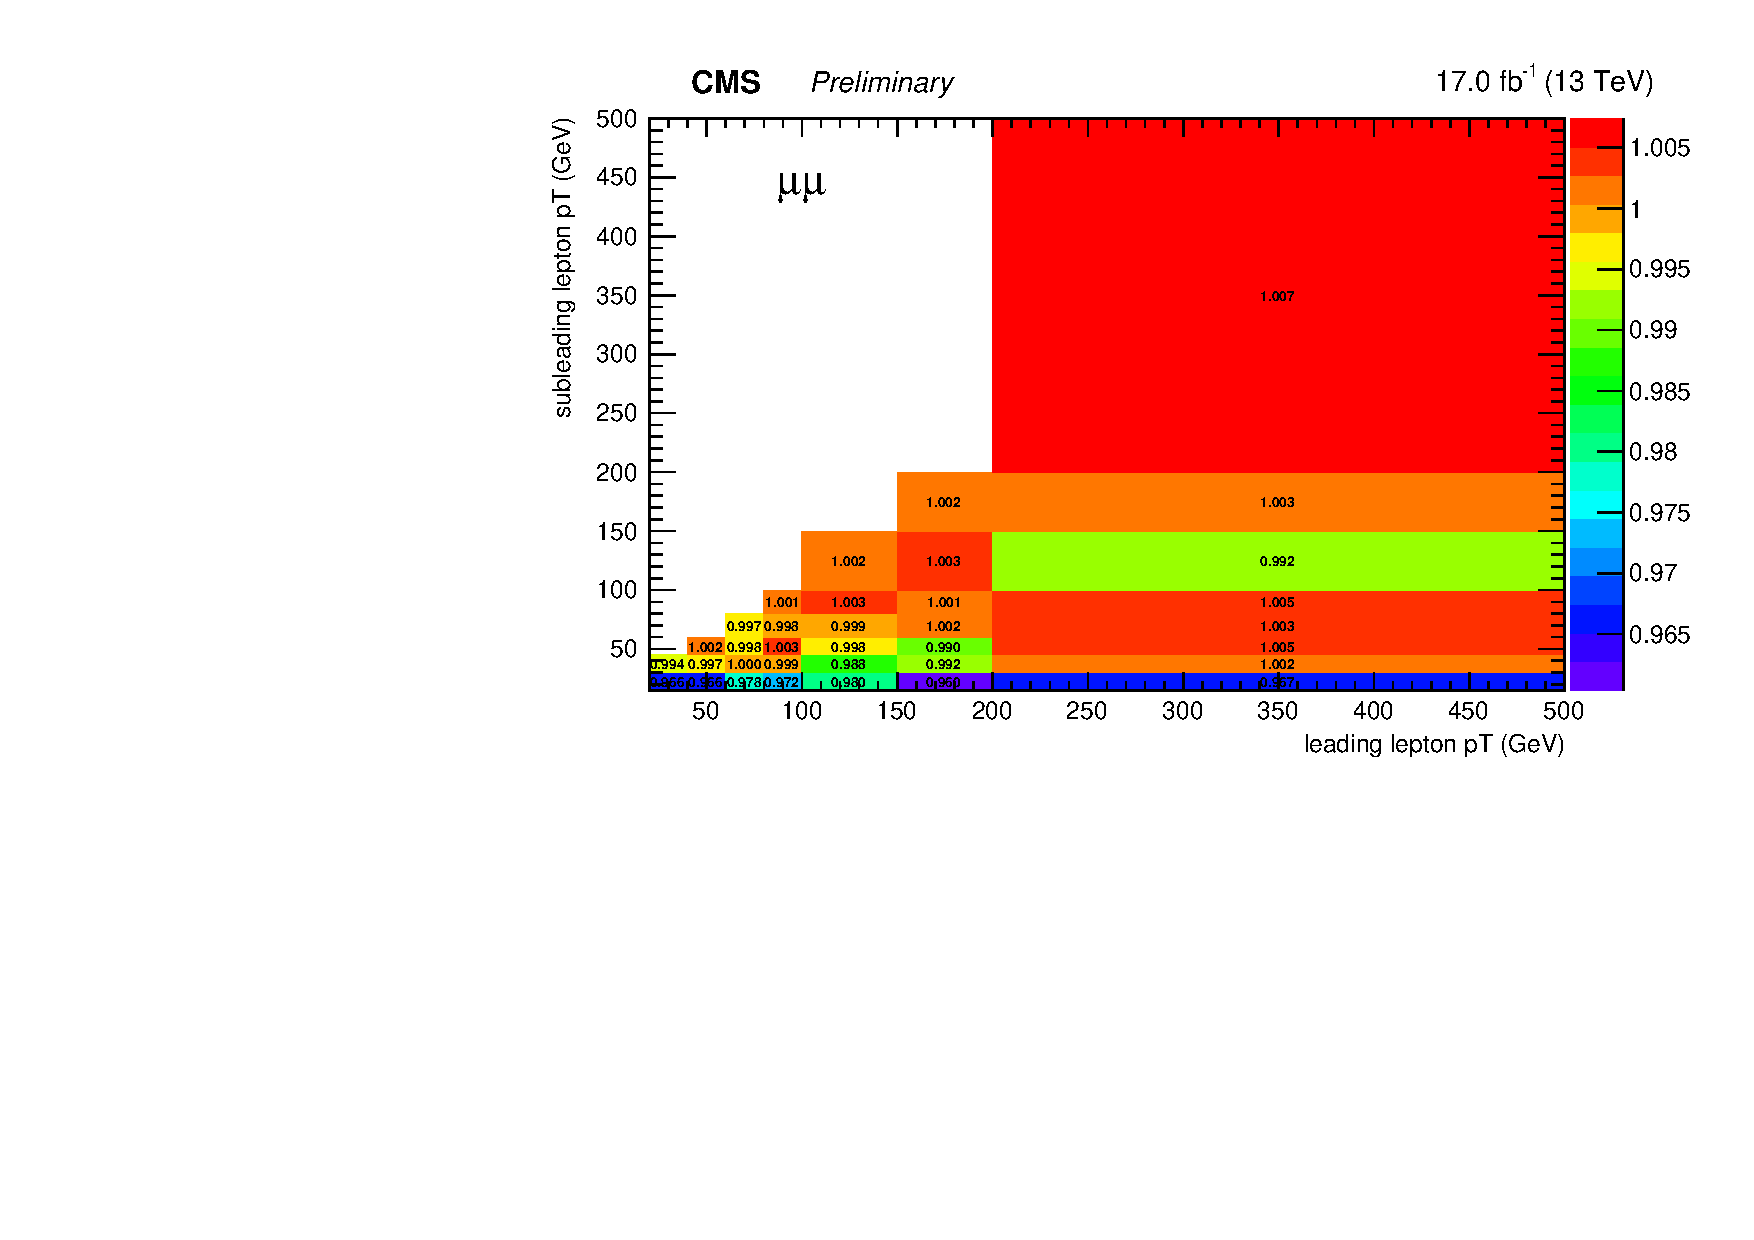
\includegraphics[width=0.50\textwidth]{fig_2016postVFP_TrigSF/h2D_lepABpt_mumu.pdf}
      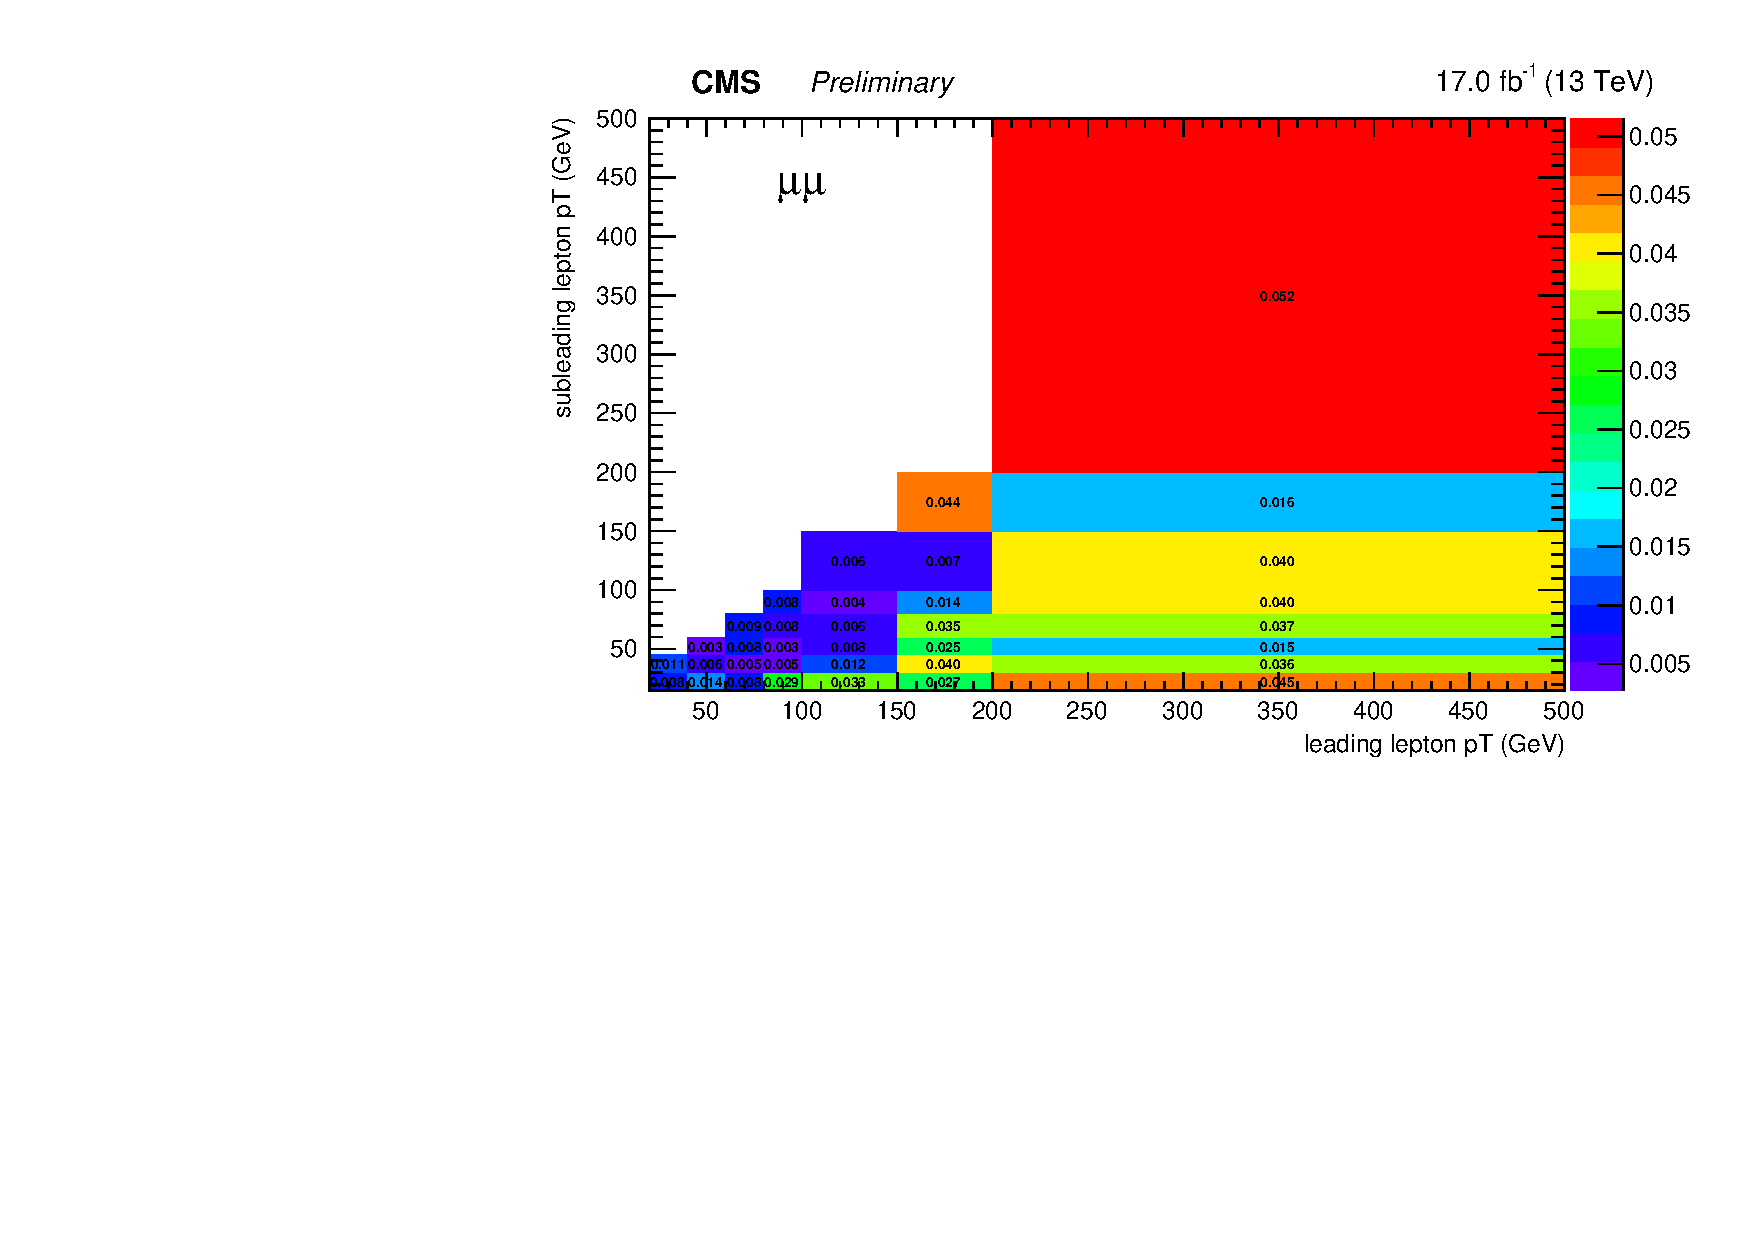
\includegraphics[width=0.50\textwidth]{fig_2016postVFP_TrigSF/h2D_lepABpt_mumu_BinErrors.pdf}\\
    \end{tabular}
    \caption{2D scale factors (Left) and total uncertainties (Right) for the 2016postVFP data set in the \emu (top), \ee (middle) and \mumu (bottom) channels as a function of leading lepton \pT and sub-leading lepton \pT.}
    \label{TrigSF_2016postVFP_4}
  \end{center}
\end{figure}

\clearpage
\subsection{Trigger Efficiencies and Scale Factors: 2017}
\label{TrigSFResults2017}

\begin{figure}[h]
  \begin{center}
    \begin{tabular}{ccc}
      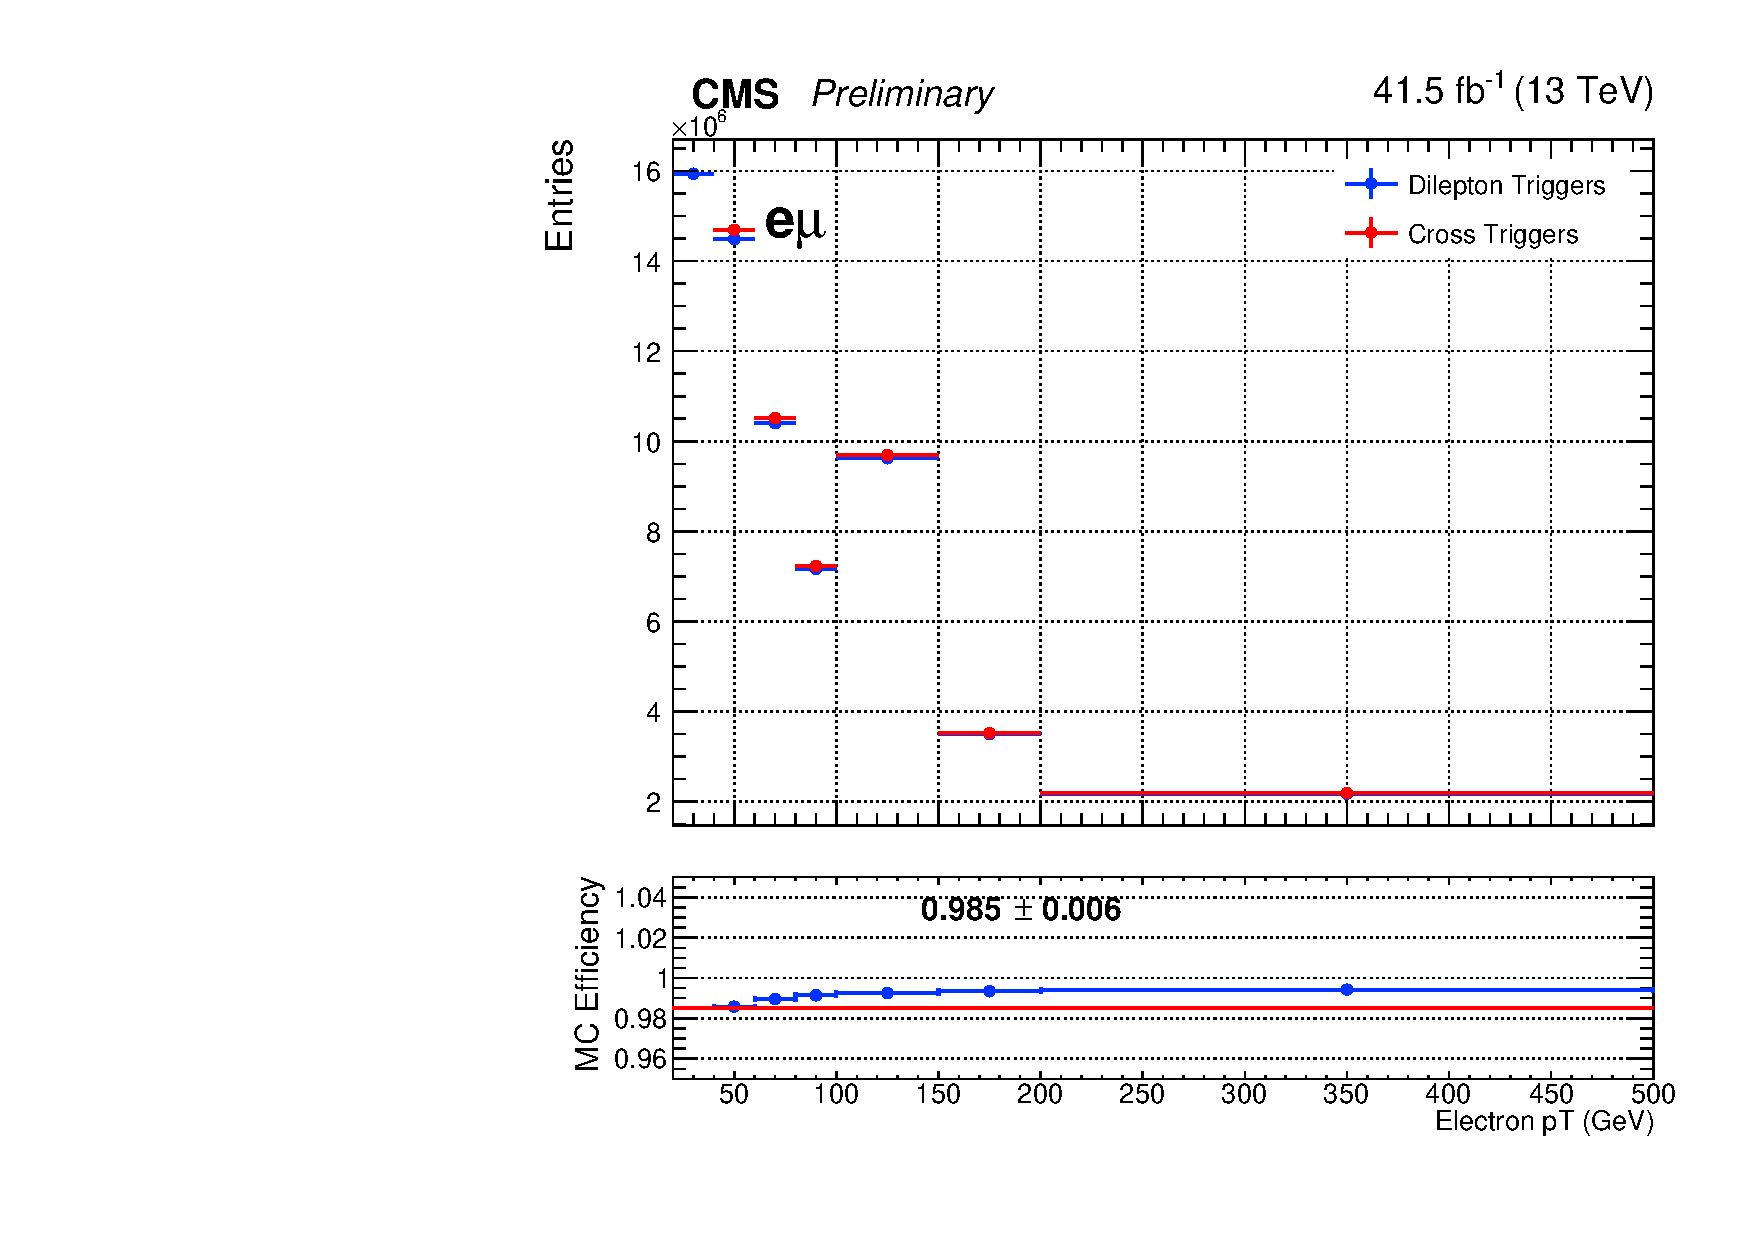
\includegraphics[width=0.32\textwidth]{fig_2017_TrigSF/g_lepApt_emu_MC.pdf}
      \includegraphics[width=0.32\textwidth]{fig_2017_TrigSF/g_lepApt_emu_data.pdf}
      \includegraphics[width=0.32\textwidth]{fig_2017_TrigSF/g_emu_lepApt_FullSystUncBand.pdf}\\
      \includegraphics[width=0.32\textwidth]{fig_2017_TrigSF/g_lepBpt_emu_MC.pdf}
      \includegraphics[width=0.32\textwidth]{fig_2017_TrigSF/g_lepBpt_emu_data.pdf}
      \includegraphics[width=0.32\textwidth]{fig_2017_TrigSF/g_emu_lepBpt_FullSystUncBand.pdf}\\
    \end{tabular}
    \caption{Efficiencies and scale factors for the 2017 data set in the \emu channel as a function of electron and muon \pT.
            The error bars indicate the statistical uncertainty, and the shaded band corresponds to the systematic uncertainty.
            }
    \label{TrigSF_2017_1}
  \end{center}
\end{figure}

\begin{figure}[h]
  \begin{center}
    \begin{tabular}{ccc}
      \includegraphics[width=0.32\textwidth]{fig_2017_TrigSF/g_lepApt_ee_MC.pdf}
      \includegraphics[width=0.32\textwidth]{fig_2017_TrigSF/g_lepApt_ee_data.pdf}
      \includegraphics[width=0.32\textwidth]{fig_2017_TrigSF/g_ee_lepApt_FullSystUncBand.pdf}\\
      \includegraphics[width=0.32\textwidth]{fig_2017_TrigSF/g_lepBpt_ee_MC.pdf}
      \includegraphics[width=0.32\textwidth]{fig_2017_TrigSF/g_lepBpt_ee_data.pdf}
      \includegraphics[width=0.32\textwidth]{fig_2017_TrigSF/g_ee_lepBpt_FullSystUncBand.pdf}\\
    \end{tabular}
    \caption{Efficiencies and scale factors for the 2017 data set in the \ee channel as a function of leading and sub-leading lepton \pT.
            The error bars indicate the statistical uncertainty, and the shaded band corresponds to the systematic uncertainty.
            }
    \label{TrigSF_2017_2}
  \end{center}
\end{figure}

\begin{figure}[h]
  \begin{center}
    \begin{tabular}{ccc}
      \includegraphics[width=0.32\textwidth]{fig_2017_TrigSF/g_lepApt_mumu_MC.pdf}
      \includegraphics[width=0.32\textwidth]{fig_2017_TrigSF/g_lepApt_mumu_data.pdf}
      \includegraphics[width=0.32\textwidth]{fig_2017_TrigSF/g_mumu_lepApt_FullSystUncBand.pdf}\\
      \includegraphics[width=0.32\textwidth]{fig_2017_TrigSF/g_lepBpt_mumu_MC.pdf}
      \includegraphics[width=0.32\textwidth]{fig_2017_TrigSF/g_lepBpt_mumu_data.pdf}
      \includegraphics[width=0.32\textwidth]{fig_2017_TrigSF/g_mumu_lepBpt_FullSystUncBand.pdf}\\
    \end{tabular}
    \caption{Efficiencies and scale factors for the 2017 data set in the \mumu channel as a function of leading and sub-leading lepton \pT.
            The error bars indicate the statistical uncertainty, and the shaded band corresponds to the systematic uncertainty.
            }
    \label{TrigSF_2017_3}
  \end{center}
\end{figure}

\begin{figure}[h]
  \begin{center}
    \begin{tabular}{cc}
      \includegraphics[width=0.50\textwidth]{fig_2017_TrigSF/h2D_lepABpt_emu.pdf}
      \includegraphics[width=0.50\textwidth]{fig_2017_TrigSF/h2D_lepABpt_emu_BinErrors.pdf}\\       
      \includegraphics[width=0.50\textwidth]{fig_2017_TrigSF/h2D_lepABpt_ee.pdf}
      \includegraphics[width=0.50\textwidth]{fig_2017_TrigSF/h2D_lepABpt_ee_BinErrors.pdf}\\
      \includegraphics[width=0.50\textwidth]{fig_2017_TrigSF/h2D_lepABpt_mumu.pdf}
      \includegraphics[width=0.50\textwidth]{fig_2017_TrigSF/h2D_lepABpt_mumu_BinErrors.pdf}\\
    \end{tabular}
    \caption{2D scale factors (Left) and total uncertainties (Right) for the 2017 data set in the \emu (top), \ee (middle) and \mumu (bottom) channels as a function of leading lepton \pT and sub-leading lepton \pT.}
    \label{TrigSF_2017_4}
  \end{center}
\end{figure}

\clearpage
\subsection{Trigger Efficiencies and Scale Factors: 2018}
\label{TrigSFResults2018}

\begin{figure}[h]
  \begin{center}
    \begin{tabular}{ccc}
      \includegraphics[width=0.32\textwidth]{fig_2018_TrigSF/g_lepApt_emu_MC.pdf}
      \includegraphics[width=0.32\textwidth]{fig_2018_TrigSF/g_lepApt_emu_data.pdf}
      \includegraphics[width=0.32\textwidth]{fig_2018_TrigSF/g_emu_lepApt_FullSystUncBand.pdf}\\
      \includegraphics[width=0.32\textwidth]{fig_2018_TrigSF/g_lepBpt_emu_MC.pdf}
      \includegraphics[width=0.32\textwidth]{fig_2018_TrigSF/g_lepBpt_emu_data.pdf}
      \includegraphics[width=0.32\textwidth]{fig_2018_TrigSF/g_emu_lepBpt_FullSystUncBand.pdf}\\
    \end{tabular}
    \caption{Efficiencies and scale factors for the 2018 data set in the \emu channel as a function of electron and muon \pT.
            The error bars indicate the statistical uncertainty, and the shaded band corresponds to the systematic uncertainty.
            }
    \label{TrigSF_2018_1}
  \end{center}
\end{figure}

\begin{figure}[h]
  \begin{center}
    \begin{tabular}{ccc}
      \includegraphics[width=0.32\textwidth]{fig_2018_TrigSF/g_lepApt_ee_MC.pdf}
      \includegraphics[width=0.32\textwidth]{fig_2018_TrigSF/g_lepApt_ee_data.pdf}
      \includegraphics[width=0.32\textwidth]{fig_2018_TrigSF/g_ee_lepApt_FullSystUncBand.pdf}\\
      \includegraphics[width=0.32\textwidth]{fig_2018_TrigSF/g_lepBpt_ee_MC.pdf}
      \includegraphics[width=0.32\textwidth]{fig_2018_TrigSF/g_lepBpt_ee_data.pdf}
      \includegraphics[width=0.32\textwidth]{fig_2018_TrigSF/g_ee_lepBpt_FullSystUncBand.pdf}\\
    \end{tabular}
    \caption{Efficiencies and scale factors for the 2018 data set in the \ee channel as a function of leading and sub-leading lepton \pT.
            The error bars indicate the statistical uncertainty, and the shaded band corresponds to the systematic uncertainty.
            }
    \label{TrigSF_2018_2}
  \end{center}
\end{figure}

\begin{figure}[h]
  \begin{center}
    \begin{tabular}{ccc}
      \includegraphics[width=0.32\textwidth]{fig_2018_TrigSF/g_lepApt_mumu_MC.pdf}
      \includegraphics[width=0.32\textwidth]{fig_2018_TrigSF/g_lepApt_mumu_data.pdf}
      \includegraphics[width=0.32\textwidth]{fig_2018_TrigSF/g_mumu_lepApt_FullSystUncBand.pdf}\\
      \includegraphics[width=0.32\textwidth]{fig_2018_TrigSF/g_lepBpt_mumu_MC.pdf}
      \includegraphics[width=0.32\textwidth]{fig_2018_TrigSF/g_lepBpt_mumu_data.pdf}
      \includegraphics[width=0.32\textwidth]{fig_2018_TrigSF/g_mumu_lepBpt_FullSystUncBand.pdf}\\
    \end{tabular}
    \caption{Efficiencies and scale factors for the 2018 data set in the \mumu channel as a function of leading and sub-leading lepton \pT.
            The error bars indicate the statistical uncertainty, and the shaded band corresponds to the systematic uncertainty.
            }
    \label{TrigSF_2018_3}
  \end{center}
\end{figure}

\begin{figure}[h]
  \begin{center}
    \begin{tabular}{cc}
      \includegraphics[width=0.50\textwidth]{fig_2018_TrigSF/h2D_lepABpt_emu.pdf}
      \includegraphics[width=0.50\textwidth]{fig_2018_TrigSF/h2D_lepABpt_emu_BinErrors.pdf}\\       
      \includegraphics[width=0.50\textwidth]{fig_2018_TrigSF/h2D_lepABpt_ee.pdf}
      \includegraphics[width=0.50\textwidth]{fig_2018_TrigSF/h2D_lepABpt_ee_BinErrors.pdf}\\
      \includegraphics[width=0.50\textwidth]{fig_2018_TrigSF/h2D_lepABpt_mumu.pdf}
      \includegraphics[width=0.50\textwidth]{fig_2018_TrigSF/h2D_lepABpt_mumu_BinErrors.pdf}\\
    \end{tabular}
    \caption{2D scale factors (Left) and total uncertainties (Right) for the 2018 data set in the \emu (top), \ee (middle) and \mumu (bottom) channels as a function of leading lepton \pT and sub-leading lepton \pT.}
    \label{TrigSF_2018_4}
  \end{center}
\end{figure}

\clearpage
\newpage
\section{Search for Lorentz Invariance Violation in \ttbar Production}
Lorentz symmetry, i.e. that the laws of physics are the same in all inertial frames of reference, is a fundamental principle of general relativity and relativistic quantum field theories.
The search for violation of Lorentz symmetry involves looking for deviations from this symmetry, which could indicate the presence of new physics Beyond the Standard Model (BSM).
One method to test the validity of Lorentz symmetry is to search for a modulation of the \ttbar cross section as a function of sidereal time (the orientation of the experiment relative to the fixed position of stars in the sky).
In order to accommodate a search and provide time dependence, the dilepton trigger efficiency scale factors were measured 1-Dimensionally as a function of sidereal time using the same method outlined above, with the exception of not including the number of vertices partition as a source of event topology systematic uncertainty.
\subsection{Translating UNIX Time to Sidereal Time}
Every CMS data event is recorded with a UNIX timestamp. 
The sidereal day, which is the time it takes for one rotation of the Earth relative to the stars, is about four minutes shorter than the solar day, which is the time it takes for one rotation of the Earth relative to the Sun.
In UNIX time, the rotational period of the earth (sidereal day) lasts approximately 23h 56min 4s, i.e. 86164 UNIX seconds. 
The sidereal second is defined in such a way that the rotational period of the earth is exactly 24h, i.e. 86400 sidereal seconds.
The following formula is used to translate UNIX time to sidereal time:
\begin{equation}
\Omega_{sidereal} t_{sidereal} = \Omega_{UTC} \times (t_{UNIX} - t_0) + \phi_{UNIX} + \phi_{longitude}
\end{equation}
In this equation:
\begin{itemize}
\item $\Omega_{sidereal}$ is the angular velocity of earth's rotation around its axis in sidereal time: $\Omega_{sidereal} = 2\pi / 86400 s^{-1}$ (sidereal). 
\item $\Omega_{UTC}$ is the angular velocity of earth's rotation around its axis in UTC time: $\Omega_{UTC} = 2\pi / 86164 s^{-1}$ (UTC). 
\item $t_{UNIX}$ is the event timestamp recorded at CMS, in UNIX time; this is the number of UTC seconds since the UNIX epoch, i.e. the 1st of January 1970. However, handling large number of seconds is sometimes not practical and a $t_0$ origin is subtracted to set the origin at the first second of 2016.
\item The azimuth angle $\phi_{UNIX}$ encodes the phase between the Unix epoch and "J2000", which is the origin of sidereal time count. J2000 is defined as the direction pointed by the crossing of ecliptic and equator plans, at noon the 1st of January 2000, on the side of the earth were the Sun moves from the Southern hemisphere to the Northern hemisphere. 
\item The azimuth $\phi_{longitude}$ is the effective longitude of the beam at CMS relative to the Greenwich meridian, in radians.
\end{itemize}

\clearpage
\newpage
\subsection{Time Dependent Trigger Scale Factors: 2016}
\label{TrigSFResults_SideReal_2016}

\begin{figure}[h]
  \begin{center}
    \begin{tabular}{cc}
      \includegraphics[width=0.32\textwidth]{fig_2016_sidereal/g_emu_sidereel_FullSystUncBand.pdf}
      \includegraphics[width=0.50\textwidth]{fig_2016_sidereal/g_emu_sidereel_ErrorsBreakdown.pdf}\\
    \end{tabular}
    \caption{Trigger scale factors for the 2016 data set in the \emu channel as a function of sidereal time.
            The error bars indicate the statistical uncertainty, and the shaded band corresponds to the systematic uncertainty.
            }
    \label{TrigSF_SideReal_2016_1}
  \end{center}
\end{figure}

\newpage
\subsection{Time Dependent Trigger Scale Factors: 2017}
\label{TrigSFResults_SideReal_2017}

\begin{figure}[h]
  \begin{center}
    \begin{tabular}{cc}
      \includegraphics[width=0.32\textwidth]{fig_2017_sidereal/g_emu_sidereal_FullSystUncBand.pdf}
      \includegraphics[width=0.50\textwidth]{fig_2017_sidereal/g_emu_sidereal_ErrorsBreakdown.pdf}\\
    \end{tabular}
    \caption{Trigger scale factors for the 2017 data set in the \emu channel as a function of sidereal time.
            The error bars indicate the statistical uncertainty, and the shaded band corresponds to the systematic uncertainty.
            }
    \label{TrigSF_SideReal_2017_1}
  \end{center}
\end{figure}
\ProvidesFile{appendices/ap-FastTiming.tex}

\chapter{UTILIZING INDUCED CURRENTS FOR FAST TIMING INFORMATION IN PIXEL DETECTORS TO ACHIEVE FOUR-DIMENSIONAL TRACKING}

\section{Overview and Motivation}
To increase the physics reach potential of high energy collision experiments, the HL-LHC upgrade aims to vastly increase the instantaneous luminosity of the LHC beyond its current value. 
As instantaneous collider luminosity increases, silicon pixel tracking detectors in HL-LHC experiments are faced with the challenge of resolving the trajectories of high energy particles in environments with high pileup, rate, and radiation.
With an expected pileup of up to 200 events per bunch crossing at the HL-LHC, with an average distance between vertices \sim$\SI{500}{\micron}$ and timing rms \sim$\SI{150}{\ps}$~\cite{CARTIGLIA201747}, precise timing information would dramatically improve the reconstruction process by providing another dimension to separate vertices and avoid a loss of events due to pileup degradation.

To achieve precise timing measurements for HL-LHC collision, the CMS collaboration has designed the MIP timing sub-detector (MTD) to measure arrival times of high-energy particles~\cite{CMS:2667167}.
The hybrid design of the MTD places LYSO scintillating crystals read-out by silicon photo-multipliers (SiPM) in the barrel, as well as low gain avalanche diodes (LGADs) in the end-caps, between the silicon tracker and ECAL layers, to complement timing information provided by the ECAL and provide time-of-flight information with timing resolutions on the order of a few tens of picoseconds.

Hybrid silicon pixel detectors consisting of silicon sensors bump-bonded to readout chips currently constitute state of the art silicon tracking detector technology and are the front-runners for track reconstruction and vertex identification in the high instantaneous luminosity environment of the HL-LHC.
While these detectors have high granularity for spatial measurements, the timing resolution is relatively poor, because the sensors and readout electronics have cumbersome interconnects with high capacitance additions to the pre-amplifiers. 
Pixel detectors able to provide four-dimensional information for tracking have not yet been realized.

\section{Small Pixels, Signal, and Noise}
Collaborating with FNAL scientist Dr. Ron Lipton, we explore whether small, low capacitance pixels integrated with fast electronics show promise for realizing the timing resolution required for four-dimensional tracking.
Smaller pixels provide better resolution, better efficiency by avoiding in-pixel pileup, and have higher radiation tolerance due to less leakage current per pixel~\cite{Garcia-Sciveres_2018}.

\begin{figure}[!htb]
  \begin{center}
    \begin{tabular}{c}
        \includegraphics[width=0.45\textwidth]{fig_FastTiming/Jitter.png}
    \end{tabular}
    \caption{Fluctuations in signal amplitude crossing a voltage threshold translate into timing fluctuations called "jitter."
            }            
    \label{Jitter}
  \end{center}
\end{figure}
The timing resolution ($\sigma_t$) in a system limited by "jitter," i.e. early or late firing fluctuations due to the presence of noise~\ref{Jitter}, can be expressed as:
\begin{linenomath*}
\begin{align}
\sigma_t =\frac{\sigma_n}{\frac{d V}{d t}\vert_{V_T}} \approx t_r\frac{Noise}{Signal}
\end{align}
\end{linenomath*}
where $\sigma_n$ is the front-end system noise, $\frac{d V}{d t}\vert_{V_T}$ is the slope of the signal at the threshold, and $t_r$ is the rise time of the signal to the threshold crossing~\cite{4336333}.
The system noise is proportional the load capacitance, and the inverse square root of the input transistor conductance, i.e. $\sigma_n \propto \frac{C_L}{g_m}$.
Therefore, maximizing signal to noise, minimizing rise times $t_r$, increasing $g_m$, and minimizing load capacitance $C_L$ yield better timing resolutions.
The LGAD approach to this challenge is to use moderate gain to increase the signal~\cite{SADROZINSKI2013226}, but we consider the approach of minimizing rise times and load capacitance.

\section{Three-Dimensional Integration}
For the noise component of minimizing jitter, three-dimensional integrated circuit (3DIC) technologies show promise for efforts towards realizing the timing resolution required for four-dimensional tracking by enabling fine pitch, low capacitance bonding and interconnects as a replacement to bump-bonding for hybrid silicon pixel detectors~\cite{7167712,7027258}. 
The hybrid Ziptronix direct bonding interconnect (DBI) technique bonds planarized silicon wafers and electrically connects layers via the insertion of through silicon vias (TSV). 
Due to lower load capacitance, a hybrid, (DBI) bonded VIPIC three-dimensional prototype assembly demonstrated nearly a factor of two decrease in noise~\ref{FusionBondedNoise_PixelPitchCapacitance} relative to a bump-bonded assembly~\cite{Lipton:2018mqk}.  
Moreover, TCAD simulations predict that smaller pixel pitch results in lower detector capacitance.
\begin{figure}[!htb]
  \begin{center}
    \begin{tabular}{cc}
        \includegraphics[width=0.45\textwidth]{fig_FastTiming/FusionBondedNoise.png}
        \includegraphics[width=0.35\textwidth]{fig_FastTiming/PixelPitch_Capacitance.png}
    \end{tabular}
    \caption{The noise in hybrid bonded VIPIC three-dimensional assembly is almost a factor of two lower than the equivalent conventionally bump bonded parts due to lower $C_L$ (Left).
            TCAD simulations predict that smaller pixel pitch results in lower detector capacitance (Right).
            }            
    \label{FusionBondedNoise_PixelPitchCapacitance}
  \end{center}
\end{figure}
In general, 3DIC technologies have many potential implementations for integrating silicon sensors with dense readout electronics, with advantages including radiation hardness, low mass, and decreasing costs, that could make them ideally suited for application in high-energy particle silicon pixel detectors.

\section{Induced Currents for Fast Timing}
Signal current, as registered by an electrode, begins before any charge is collected by the electrode.  
Current is instantaneously induced in the electrode as electrostatic flux lines ending on the electrode change due to charges moving in the vicinity~\cite{doi:10.1063/1.1710367}.
According to the Ramo-Shockley theorem, current induced on an electrode in a multi-electrode system can be calculated from the coupling between the moving charge and the electrode, using a "weighting field," depending on geometry and doping, that is determined by setting the potential of the electrode under consideration to unity, and setting the potential of all other electrodes to zero~\cite{1686997}.
The instantaneous current registered by an electrode by a charge moving in the vicinity can be expressed in terms of charge $q$, velocity $\vec{v}$, and weighting field $\vec{E_W}$ as:
\begin{linenomath*}
\begin{align}
i = -q \vec{v} \cdot \vec{E_W}
\end{align}
\end{linenomath*}
Induced currents have a very fast rise time, but if the charge is not collected by the electrode under consideration, then the induced signal current will change sign and integrate to zero.
For geometries where the pixel pitch is small compared to the substrate thickness, charge moving far from the surface will induce currents in a cluster of electrodes surrounding the nodes that collect charge.
If detectors have sufficiently low capacitance and are integrated with fast electronics, the induced current signal can be utilized to provide timing information for four-dimensional tracking.

\section{FEA Simulations with TCAD}
Technology computer-aided design (TCAD) software is used to explore models for planar sensors, in order to optimize the doping and geometry to achieve large induced currents with fast rise times.
The TCAD simulation uses finite element analysis (FEA) to simulate the electrical properties and behavior of semiconductor models, in this case by calculating the electric field in the model, the weighting fields of the individual electrodes, and the current induced at each electrode due to the motion of charge carriers in the substrate.
Both three-dimensional ($3 \times 3$) and two-dimensional ($1 \times 9$) models of pixel arrays, consist ting of aluminium electrodes coupled to a silicon substrate, are simulated~\ref{Materials_Model}.
Different pixel pitches (\SI{25}{\micron} - \SI{100}{\micron}), substrate thicknesses (\SI{50}{\micron} - \SI{300}{\micron}), doping schemes ($n$-on-$n$, $n$-on-$p$), and bias voltages (\SI{100}{\V} - \SI{400}{\V}) were considered for these simulations.
Electrons are the preferred charge carrier, as they have higher mobility than holes and thus higher velocity, inducing larger currents for the same electric field strength.
Even in the absence of an externally applied voltage, every $pn$-junction has a "built-in" electric field between the $p$ and $n$ sides from thermal diffusion of mobile charge carriers.
For the doping scheme, $n$-on-$n$ has a maximal electric field near the bottom-side, whereas $n$-on-$p$ has a maximal electric field near the top~\ref{Doping_ElectricField}.
Intermediate p-regions between electrodes, called "$p$-stops," help shape the electric field and prevent unwanted diffusion of charges away from collecting electrodes.
\begin{figure}[!htb]
  \begin{center}
    \begin{tabular}{cc}
      \includegraphics[width=0.45\textwidth]{fig_FastTiming/Materials.png}
      \includegraphics[width=0.275\textwidth]{fig_FastTiming/Model3D.png}
    \end{tabular}
    \caption{Two-dimensional $1 \times 9$ (Left) and three-dimensional $3 \times 3$ (Right) models of \SI{25}{\micron} pitch pixel arrays, consisting of aluminium electrodes (labeled) coupled to a silicon substrate.
            }
    \label{Materials_Model}
  \end{center}
\end{figure}
\begin{figure}[!htb]
  \begin{center}
    \begin{tabular}{cc}
      \includegraphics[width=0.45\textwidth]{fig_FastTiming/Net_Doping_nonn.png}
      \includegraphics[width=0.45\textwidth]{fig_FastTiming/ElectricField_nonn.png} \\
      \includegraphics[width=0.45\textwidth]{fig_FastTiming/Net_Doping_nonp.png}
      \includegraphics[width=0.45\textwidth]{fig_FastTiming/ElectricField_nonp.png} \\
    \end{tabular}
    \caption{Doping (Left) and "built-in" electric field (Right) profiles for TCAD simulated models of $1 \times 9$ (two-dimensional) array of pixels with 25 \si{\micron} pitch between aluminium electrodes coupled to a silicon substrate.
            $n$-on-$n$ (Top) has an electric field maximal near the bottom-side, whereas $n$-on-$p$ (Bottom) has an electric field maximal near the top.
            }
    \label{Doping_ElectricField}
  \end{center}
\end{figure}

Two kinds of pulses were injected into the bulk of the substrate, either localized at a specific depth to simulate an absorbed x-ray, or uniformly through the depth at an angle of incidence to simulate ionization due to a MIP traversing the sensor.
Current density profiles visualizing the motion of mobile charges after ionization are shown in figures~\ref{CurrentDensity_xray} and~\ref{CurrentDensity_MIP} for an absorbed x-ray and MIP, respectively.
Simulated signal currents induced on electrodes by a locally ionizing x-ray at various depths and by uniformly ionizing MIPs at various angles of incidence are shown in figures~\ref{Signal_xray_Multi} and~\ref{Signal_MIP_Multi}, respectively.
The rich diversity of signal shapes in figure~\ref{Signal_MIP_Multi} demonstrate that thick detectors with small pixels have potential for distinguishing tracks as a function of angle of incidence by using information from the collective pulse shapes of nearby pixels. 
The time between the initial current pulse and the peak current in a set of pixel shapes, for example, could be correlated in the readout electronics to measure the track angle.

\begin{figure}[!htb]
  \begin{center}
    \begin{tabular}{c}
        \includegraphics[width=.90\textwidth]{fig_FastTiming/CurrentDensity_xray.png}
    \end{tabular}
    \caption{Current density profiles visualizing the motion of mobile charges after localized ionization by an absorbed x-ray:
            .1 \si{\ns} (Top Left), .5 \si{\ns} (Top Middle), 1 \si{\ns} (Top Right), 1.5 \si{\ns} (Bottom Left), 2.0 \si{\ns} (Bottom Middle), 2.5 \si{\ns} (Bottom Right).
            The electrons drift upward towards the electrodes, and the holes drift downward.
            }
    \label{CurrentDensity_xray}
  \end{center}
\end{figure}
\begin{figure}[!htb]
  \begin{center}
    \begin{tabular}{c}
        \includegraphics[width=.90\textwidth]{fig_FastTiming/CurrentDensity_MIP.png}
    \end{tabular}
    \caption{Current density profiles visualizing the motion of mobile charges after uniform ionization at a 15 degree angle of incidence by a MIP:
            .1 \si{\ns} (Top Left), .5 \si{\ns} (Top Middle), 1 \si{\ns} (Top Right), 1.5 \si{\ns} (Bottom Left), 2.0 \si{\ns} (Bottom Middle), 2.5 \si{\ns} (Bottom Right).
            The electrons drift upward towards the electrodes, and the holes drift downward.
            }
    \label{CurrentDensity_MIP}
  \end{center}
\end{figure}

\begin{figure}[!htb]
  \begin{center}
    \begin{tabular}{c}
        \includegraphics[width=.90\textwidth]{fig_FastTiming/Signal_xray_Multi.png}
    \end{tabular}
    \caption{Currents induced on electrodes by a locally ionizing x-ray at various depths (\SI{10}{\micron}, \SI{100}{\micron}, \SI{190}{\micron}) from the central electrode of a \SI{200}{\micron} thick detector with \SI{25}{\micron} pitch pixels biased at \SI{400}{\V}.
    The ionization is localized directly below Electrode 5 (E4).
            }
    \label{Signal_xray_Multi}
  \end{center}
\end{figure}
\begin{figure}[!htb]
  \begin{center}
    \begin{tabular}{c}
        \includegraphics[width=.90\textwidth]{fig_FastTiming/Signal_MIP_Multi.png}
    \end{tabular}
    \caption{Currents induced on electrodes by a uniformly ionizing MIP at various angles of incidence with respect to the surface of a \SI{200}{\micron} thick detector with \SI{25}{\micron} pitch pixels biased at \SI{400}{\V}.
            The track at 0 degrees is incident on Electrode 5 (E4).
            }
    \label{Signal_MIP_Multi}
  \end{center}
\end{figure}

\section{Results}
The same pattern emerges that is most clearly demonstrated with the case of simulated x-ray absorption~\ref{Signal_xray}.
On the picosecond timescale, there is an initial current spike, that is similar for all nearby pixels with pitch small compared to ionization depth.
On the nanosecond timescale, charges-collecting electrodes detect a large signal current, but for electrodes not collecting charges, the current changes sign and integrates to zero.
\begin{figure}[!htb]
  \begin{center}
    \begin{tabular}{c}
      \includegraphics[width=0.50\textwidth]{fig_FastTiming/Signal_xray.png}
    \end{tabular}
    \caption{Signal for an X-ray deposited at \SI{190}{\micron} in a \SI{200}{\micron} thick detector with \SI{25}{\micron} pitch pixels biased at \SI{400}{\V}.
            }
    \label{Signal_xray}
  \end{center}
\end{figure}

The simulated currents are injected into a simulation program with integrated circuit emphasis (SPICE) model of a \SI{65}{\nm} technology amplifier, including noise, and current supplied to the input transistor around 4 $\mu A$.
The pulse shape from the central electrode peaks at \sim$\SI{1}{\V}$ after \sim$\SI{12}{\ns}$, and the edge electrode peaks at \sim$\SI{25}{\mV}$ after \sim$\SI{2}{\ns}$.
The threshold is set at \SI{130}{\mV} above baseline for the central electrode and \SI{10}{\mV} above baseline for the edge electrode.
The jitter timing resolution is extracted from a Gaussian fit of the arrival times of an ensemble of resulting pulses that differ only due to jitter noise.
\begin{figure}[!htb]
  \begin{center}
    \begin{tabular}{c}
      \includegraphics[width=0.80\textwidth]{fig_FastTiming/TimingResolutions.png}
    \end{tabular}
    \caption{Pulse shapes and jitter timing resolution, of central (charge collecting) and edge (induced current) electrodes, for a simulated x-ray ionization at a depth of \SI{185}{\micron} in a \SI{200}{\micron} thick detector.
        (a) Pulse shapes for the central and edge electrode. 
        (b) Pulse shape for the edge electrode for 25 pulses, including noise, with the threshold set at \SI{10}{\mV} above baseline.
        (c) The jitter timing resolution for the edge electrode in plot b.
        (d) The jitter timing resolution for the central electrode with a threshold of \SI{130}{\mV} above the baseline.
            }
    \label{TimingResolutions}
  \end{center}
\end{figure}

The resulting jitter time resolution~\ref{TimingResolutions} is \sim$\SI{10}{\ps}$ for central electrodes and \sim$\SI{30}{\ps}$ for edge electrodes and, which indicates that for timing resolution with small pixels, noise-induced jitter will likely not be a dominant factor.
Time walk and ionization fluctuation components of timing resolution were not considered in this limited study.

As a concluding remark, small pixel detector systems show promise for addressing some of the extreme challenges of future high-energy particle experiments, including precise position and timing resolution, complex event topology, and radiation hardness.
This study considers some toy models, but for real application of these ideas, there are many more electronics and system engineering considerations that need to be studied.





% \immediate\setlength{\bibhang}{-3in}
% \immediate\setlength{\itemindent}{3in}
% \immediate\setlength{\rightmargin}{3in}

%
% This is only done if you are using BibLaTeX.
%
\makeatletter  % commented out on 2022-01-26
  \defbibenvironment{bibliography}
    {%
      \list
        {%
          \printtext[labelnumberwidth]%
          {%
            \printfield{prefixnumber}%
            \printfield{labelnumber}%
          }%
        }%
        {%
          \setlength{\bibhang}{1in} %%%%% was 0pt
          \setlength{\itemindent}{1in}%  -\leftmargin} %%%%% was 0pt
          \setlength{\itemsep}{\bibitemsep}%
          \setlength{\leftmargin}{0pt}%  .22in} % 0.42in}
          \setlength{\parsep}{\bibparsep}%
           \setlength{\rightmargin}{0.33in}%
        }%
    }
    {\endlist}
    {\item}
\makeatother  % commented out on 2022-01-26

% \immediate\setlength{\labelnumberwidth}{1.5in} %%%%% was commented out
\setlength{\labelwidth}{1.5in}
\def\sllnsez{[999] }

{%
  % Make _ in URLs visible.
  % \def\t{\char'137}%
  \catcode`*=\active
  \def*{\char'137}%  \char'137 is _
  \PrintBibliography
}


% My filename conventions:
%     FILE THAT START WITH    ARE
%     ap-                     appendices
%     ch-                     chapters
%     gr-                     graphics
%     pa-                     packages
%     z                       temporary files

% LaTeX won't read after the \end{document} command.
% You can put notes to yourself or LaTeX input not
% ready for use after "\end{document}" if you'd like.
\end{document}
